% Paul M. Garrett Thesis 2019
% Chapters
% 1 -- Introduction to Numbers
% 2 -- Estimation, SFT and NDE
        % - Estimation
        % - Cognitive Properties
        % - SFT
        % - Pilot Studies 1 & 2
        % - Results
        % - Discussion
% 3 -- Estimation Systems
        % - Method - Estimation with SFT
        % - Results - Heir MIC and Bayes SIC
        % - Discussion
% 4 -- Subitizing Systems
        % - Subitizing
        % - Method
        % - Results
        % - Discussion
% 5 -- Mixture Models of Parallel vs Serial
        % Theory
        % Simulation
        % Discussion
% 6 -- Symbolic Wheel Task
        % Ideal Observer Analysis
        % Method
        % Results
        % Discussion
% 7 -- Cross Cultural Wheel Task
        % Dots - Intro to Symbolic Numbers
        % English, Chinese & Thai - Digits vs Dots
        % Understanding Number <--> Perception of Number
        % Multidimensional Scaling
            % Bias
            % Luce Choice Model
            % Unbias MDS
        % Method - Wheel Task
        % English Cohort - Results
        % Chinese Cohort - Results
        % Discussion
% 8 -- General Discussion 
    % - Discussion of Numbers & Quantity 
    % - Implications of PhD Work
    % - Future Research
    % - Conclusions

\documentclass[12pt,oneside]{Thesis}
\graphicspath{{}}

\usepackage{epigraph}
\setlength\epigraphwidth{.5\textwidth}
\usepackage{indentfirst}
\usepackage{apacite}
\usepackage{tipa}
\usepackage[english]{babel}
\usepackage{booktabs}
\usepackage{setspace}
\usepackage{amsmath}
\usepackage{amssymb}
\usepackage{amsthm}
\usepackage{graphicx}
\usepackage{multirow}
\usepackage[colorinlistoftodos]{todonotes} 
\hypersetup{urlcolor=black, colorlinks=true} 
\usepackage{parskip}
\usepackage[utf8]{inputenc}
\usepackage{hhline}
\usepackage{hyperref}

\usepackage{CJKutf8}
\usepackage{lineno} 
\usepackage{float}
\usepackage{longtable}

\usepackage{xcolor}
\usepackage{soul}

\usepackage{atbegshi,etoolbox}

\newcommand{\discardpages}[1]{% \discardpages{<csv list>}
  \xdef\discard@pages{#1}% Store pages to discard
  \AtBeginShipout{% At shipout, decide whether to discard page/not
    \renewcommand*{\do}[1]{% How to handle each page entry in csv list
      \ifnum\value{page}=##1\relax%
        \AtBeginShipoutDiscard% Discard page/not
        \gdef\do####1{}% Do nothing further
      \fi%
    }%
    \expandafter\docsvlist\expandafter{\discard@pages}% Process list of pages to discard
  }%
}
\newif\ifkeeppage
\newcommand{\keeppages}[1]{% \keeppages{<csv list>}
  \xdef\keep@pages{#1}% Store pages to keep
  \AtBeginShipout{% At shipout, decide whether to discard page/not
    \keeppagefalse%
    \renewcommand*{\do}[1]{% How to handle each page entry in csv list
      \ifnum\value{page}=##1\relax%
        \keeppagetrue% Page should be kept
        \gdef\do####1{}% Do nothing further
      \fi%
    }%
    \expandafter\docsvlist\expandafter{\keep@pages}% Process list of pages to keep
    \ifkeeppage\else\AtBeginShipoutDiscard\fi% Discard page/not
  }%
}

%%% Remove pages to make a separate doc for Sup Materials
%\discardpages{244, 245, 246, 247, 248, 249, 250, 251, 252, 253, 254, 255, 256, 257, 258, 259, 260, 261, 262, 263, 264, 265, 266, 267, 268, 269, 270, 271, 272, 273, 274, 275, 276, 277, 278, 279, 280, 281, 282, 283, 284, 285, 286, 287, 288, 289, 290, 291, 292, 293, 294, 295, 296, 297, 298, 299, 300, 301, 302, 303, 304, 305, 306, 307, 308, 309, 310, 311, 312, 313, 314, 315, 316, 317, 318, 319, 320, 321, 322, 323, 324, 325, 326, 327, 328, 329, 330}

%\keeppages{244, 245, 246, 247, 248, 249, 250, 251, 252, 253, 254, 255, 256, 257, 258, 259, 260, 261, 262, 263, 264, 265, 266, 267, 268, 269, 270, 271, 272, 273, 274, 275, 276, 277, 278, 279, 280, 281, 282, 283, 284, 285, 286, 287, 288, 289, 290, 291, 292, 293, 294, 295, 296, 297, 298, 299, 300, 301, 302, 303, 304, 305, 306, 307, 308, 309, 310, 311, 312, 313, 314, 315, 316, 317, 318, 319, 320, 321, 322, 323, 324, 325, 326, 327, 328, 329, 330}


\def\Red{black}

\raggedbottom

\newcommand{\tval}[3]{$t$(#1) = #2, $p$ #3}
\newcommand{\Fval}[4]{$F$(#1, #2) = #3, $p$ #4}
\newcommand{\mRT}[1]{$\rm{{mRT}}_{#1}$}
\newcommand{\mAcc}[1]{$\rm{\overline{Acc}}_{#1}$}
\newcommand{\rt}[2]{$\rm{mRT = #1ms, SD = #2ms}$}
\newcommand{\acc}[2]{$\rm{Err = #1, SD = #2}$}
\newcommand{\Acc}[2]{$\rm{Acc = #1, SD = #2}$}

\newcommand{\St}[1]{$\rm{S_{#1}}$($t$)}
\newcommand{\AY}[1]{$\rm{AY_{#1}}$($t$)}
\newcommand{\XB}[1]{$\rm{X_{#1}B}$($t$)}
\newcommand{\etap}[1]{$\eta_{p}^{2} = #1$}

\def\mSD{$\rm{\overline{SD}}$ }
\def\Ct{{\rm C($t$) }}
\def\CCFh{{\rm CCF$_{high}$($t$) }} 
\def\CCFl{{\rm CCF$_{low}$($t$) }}
\def\SIC{{\rm SIC($t$) }}
\def\CCF{{\rm CCF($t$) }}
\def\Rh{{\rm R$_{high}$($t$) }} 
\def\Rl{{\rm R$_{low}$($t$) }} 
\def\Rd{{\rm R$_{diff}$($t$) }} 
\def\t{{\rm \textit{t}}}
\def\Cor{{\rm C$_{OR}$($t$) }}
\def\Cand{{\rm C$_{AND}$($t$) }}
\def\SLL{{\rm S_{LL}}}
\def\SLH{{\rm S_{LH}}}
\def\SHL{{\rm S_{HL}}}
\def\SHH{{\rm S_{HH}}}


\def\eg{\rm{e.g.,} }
\def\ie{\rm{i.e.,} }


%\thesistitle{Understanding the cognitive mechanisms behind the comparison of quantities and the confusion of numbers}
\thesistitle{Understanding the Cognitive Mechanisms Behind Numerical Cognition}

\title{\ttitle}

\begin{document}

% Calls to Thesis Class
\frontmatter
\setstretch{2}
\fancyhead{}
\rhead{\thepage} 
\lhead{} 
\pagestyle{fancy}
\newcommand{\HRule}{\rule{\linewidth}{0.5mm}}
\hypersetup{pdftitle={\ttitle}}
\hypersetup{pdfsubject=\subjectname}
\hypersetup{pdfauthor=\authornames}
\hypersetup{pdfkeywords=\keywordnames}

% Thesis Title Page
\begin{titlepage}
\begin{center}
\HRule \\[.2cm] 
{\Huge \bfseries \ttitle}\\[.1cm] 
\HRule \\[1cm] 

\includegraphics[height=6cm,width=6cm]{Figures/Misc/UON.jpg}\\[.5cm] 
\large by\\
\large Paul M. Garrett B.Psych (Hons); Newcastle \\
\large Supervised by A Prof. Ami Eidels \& Prof. Scott Brown\\[.5cm]
\large A thesis submitted in fulfilment of the requirements\\ for the degree of \degreename~in Cognitive Psychology \\[0cm] 
\large \today \\[.5cm]
\large This research was supported by an Australian Government Research Training Program (RTP) Scholarship
\vfill
\end{center}
\end{titlepage}

\Declaration{
\addtocontents{toc}{\vspace{1em}} 

% Originality Statement
\begin{itemize} 
\item[\tiny{$\blacksquare$}] \emph{Originality:} I hereby certify that the work embodied in the thesis is my own work, conducted under normal supervision. The thesis contains no material which has been accepted for the award of any other degree or diploma in any university or other tertiary institution and, to the best of my knowledge and belief, contains no material previously published or written by another person, except where due reference has been made in the text. I give consent to the final version of my thesis being made available worldwide when deposited in the University’s Digital Repository**, subject to the provisions of the Copyright Act 1968. \\
**Unless an Embargo has been approved for a determined period
\item[\tiny{$\blacksquare$}] \emph{Collaboration:} I hereby certify that the work embodied in this thesis has been done in collaboration with other
researchers, or carried out in other institutions. I have included as part of the thesis a statement clearly outlining the extent of collaboration, with whom and under
what auspices.
\item[\tiny{$\blacksquare$}] \emph{Authorship:} I hereby certify that the work embodied in this thesis contains published papers/scholarly work of which I am a joint author. I have included as part of the thesis
a written statement, endorsed by my supervisor, attesting to my contribution to the joint
publication/s/scholarly work.
\end{itemize}
\vspace{2em}
Signed: \hspace{18em} Date: 2.12.2019}
\clearpage 

% Acknowledgements
\acknowledgements{\addtocontents{toc}{\vspace{1em}}
Firstly, I wish to acknowledge the outstanding mentorship provided by my primary supervisor, Associate Professor Ami Eidels. Ami has shaped me into the scientist I am today. Ami always made time for me, to guide me as a scientist, as an academic, and as a mentor to other students. Learning from him has been the greatest privilege of my PhD. It was from Ami that I learned the principles to which I aspire everyday.

\begin{center} 
\textit{``Have patience with your work. Have more with the work of others.''}

\textit{``Tell the truth and tell it simply, everything after that is their problem.''}

\textit{``Be kind. Kindness is one of the few currencies that count in research. \\Be kind to others. Be kind to yourself.''}

\end{center}

Secondly, I wish to thank my co-supervisor, Professor Scott Brown. Ever available, quick to laugh and keen to help. You contribution to this thesis cannot be measured in words, code or data; your contribution was the collaborative lab you made, the students you fostered and the support you always gave, unconditionally. 

To the Newcastle cognition lab and the students that made it a home --- Laura Wall, Caroline Kuhne, Nathan Evans, Gavin Cooper, Reilly Innes, Angus McKerral, Ashlea Rendell, J.P. Cavallaro, Asheek Shimul \& Erin Robinson --- this thesis was possible because of you. Like all students who attempt a PhD, there were days when I struggled to think, to write, and to teach. On those days (and every other) you supported me with fun, love, insight and most of all coffee. I wish to specially thank my constant companion, Zachary Howard, who was with me at every step of this journey and often reached down to help me stand tall. To Alexander Thorpe, Laura Waters and Murray Bennett, I could not have asked for better students, colleagues, and friends. It was my privilege and a source of constant pride to have taught and to have learned from each of you.

To the administration staff at the University of Newcastle --- Brendan Tisdell, Tara Magnay, Jess Fitzpatrick, and above all Danielle Storey --- thank you for your help and your friendship. Whether I was booking last minute flights, haphazardly searching for documents, or in one case, lost without accommodation in Boston, your skills, support, kindness, and genuine care were always felt and appreciated.

To Associate Professor Daniel Little and my research family at the University of Melbourne, your support has meant everything to me. In particular, I wish to thank Sarah Moneer, Christina Van-Heer, Xue Jun, Jess Marris, Jason Zhou, Gabriel Ong, Ariel Goh, Marcellin Martinie, and Felix Singleton Thorn. Your friendship, love and support have kept me sane throughout my move to Melbourne and the writing of this thesis. 

To the vast network of academics who have taught me these past four years, thank you. Although there are too many to list, I wish to thank Simon Dennis, Hyungwook Yim, James Townsend, Joseph Houpt, Daniel Little, Cheng-Ta Yang, Guy Hawkins, Philip Smith, Simon Lilburn, Emily Freeman, Kerry Charlmers, and David Landy. Above all, I wish to thank my oldest colleague, mentor and friend, Dr Patrick Cooper.

Finally, to my family back in Newcastle and in particular, my loving partner Zoe. On every step of this journey, from my Bachelors through to this thesis, I have had your unwavering support. Although my name may appear on the doctorate, this achievement is yours too.}

\clearpage 

% Publications in Thesis
\Publications{ 
\addtocontents{toc}{\vspace{1em}}
The work within this thesis has lead to the following journal articles that are either currently published, submitted, or in preparation, which I have listed with the full bibliographic citations in the order they appear in the thesis:

\begin{enumerate}
\item{Garrett, P. M., Howard, Z., Landy, D., Houpt, J. W., \& Eidels, A. (2019). Comparative Estimation Systems Perform Under Severely Limited Workload Capacity. \emph{Journal of mathematical psychology}.}

\item Little, D. R., Eidles, A., Houpt, J. W., Garrett P. M., \& Griffiths, D. W. (2018). Systems Factorial Technology analysis of mixture models. \emph{Journal of mathematical psychology}.

\item Garrett, P. M., Bennett, M., Howard, Z., Yang, C.T., Little, D., \& Eidels, A. (Under review). The cost of errors: confusion analysis and the mental representation of familiar and unfamiliar numerals. \textit{Acta Psychologica.}

\item Garrett, P. M., Yang, C.T., Howard, Z., Bennett, M., Little, D., \& Eidels, A. (In submission). The cross cultural cost of errors: the mental representation of familiar and unfamiliar numerals across cultures \textit{Frontiers}
\end{enumerate}
}
\clearpage 


\AddPublications{ \addtocontents{toc}{\vspace{1em}}
Listed are additional journal articles that are either currently published, submitted, or in preparation, which I have been involved in during my candidature:

\begin{enumerate}
\item \textbf{Garret, P. M.}, Chiam, P-Y, \& Yang, C-T. (In prep). Visual word processing efficiency for Chinese characters and English words. Planned Submission to \textit{Acta Psychologica}

\item Sreekumar, V., Evans, N. J., \textbf{Garrett, P. M.}, Yim, H., Sederberg, P., \& Dennis, S. (In Prep). Using an experience sampling approach to distinguish distance versus location-based processing in memory for when. Planned Submission to \textit{Psychonomic Bulletin \& Review}.

\item Howard, Z. L., \textbf{Garrett, P. M.}, Little, D., Townsend, J. T., \& Eidels, A. (Under review). Nice guys check twice: exhaustive processes in systems factorial technology. \textit{Psych Review}.

\item Yim, H., \textbf{Garrett, P. M.}, Baker, M., Sreekumar, V., \& Dennis, S. (Under Review). Examining dependencies among different time scales in episodic memory - an experience sampling study. \textit{Journal of memory and language.}

\item Yim, H., \textbf{Garrett, P. M.}, Baker, M., \& Dennis, S. (2019). Examining the independence of scales in episodic memory using experience sampling data. \emph{Proceedings of the 40th Annual Conference of the Cognitive Science Society}.

\item Dennis, S., \textbf{Garrett, P. M.}, Yim, H., Sreekumar, V., \& Stone, B. (2019). Privacy vs open science. \emph{Behavioural research methods}.

\item Dennis, S., Yim, H., \textbf{Garrett, P. M.}, Hamm, J., Osth, A., Sreekumar, V., \& Stone, B. (2019). A system for collecting active and passive experience sampling data. \emph{Behavioural research methods}.

\item Dennis, S., \textbf{Garrett, P. M.}, Yim, H., Hamm, J., Osth, A., Sreekumar, V., \& Stone, B. (2019). Privacy versus Open Science. In Goel, A., Seifert, C., \& Freksa, C. (Eds.) Proceedings of the 41st Annual Conference of the Cognitive Science Society. Austin, TX: Cognitive Science Society.

\item Dennis, S., Yim, H., Sreekumar, V., Evans. N., \textbf{Garrett, P. M.}, \& Sederberg, P. (2017). A hierarchical Bayesian model of ``memory for when'' based on experience sampling data. \emph{Proceedings of the 39th Annual Conference of the Cognitive Science Society.}

\item Tillman, G., Howard, Z., \textbf{Garrett, P. M.}, \& Eidels, A. (2017). The Stroop Effect From a Mixture of Reading Processes: A Fixed-Point Analysis. \emph{Proceedings of the 39th Annual Conference of the Cognitive Science Society.}

\item Cooper, P. S., \textbf{Garrett P. M.}, Rennie J. L. \& Karayanidis F. (2015) Task Uncertainty Can Account for Mixing and Switch Costs in Task-Switching. \emph{PLoS ONE.} 10(6).
\end{enumerate}
}
\clearpage

\AddConference{\addtocontents{toc}{\vspace{1em}}
\begin{enumerate}
\item \textbf{Garrett, P.M.} (2019). The PhD and beyond: Pathways into and out of, academia. Graduate research seminar. The University of Melbourne.

\item \textbf{Garrett, P.M.} (2019). The PhD and beyond! Graduate researchers in psychological sciences workshop. University of Melbourne.

\item \textbf{Garrett, P.M.}, Howard, Z., Houpt, J. W., Landy, D., \& Eidles, A. (2019). The comparison of large and small item-sets. The annual meeting of the Australian mathematical society, Melbourne.

\item \textbf{Garrett, P.M.}, Howard, Z., Houpt, J. W., Landy, D., \& Eidles, A. (2018). Estimating multiple item-sets: Harder than you think! Sydney Postgraduate Psychology Conference, University of New South Wales.

\item \textbf{Garrett, P.M.} (2018). Mathematics in Cognitive Psychology. Computer-Assisted Research Mathematics and its Applications (CARMA): mathematical thinking workshop, Newcastle.

\item \textbf{Garrett, P.M.}, Yim, H., Sreekumar, V., Evans, N., \& Dennis, S. (2018). A model for 'When' in memory. Hunter medical research institute post-graduate conference, Newcastle.

\item \textbf{Garrett, P.M.}, Yim, H., Sreekumar, V., Evans, N., \& Dennis, S. (2018). A predictive model for 'When' in human memory. Experimental Psychology Conference, Hobart.

\item \textbf{Garrett, P.M.}, Houpt, J., Landy, D., \& Eidels, A. (2018). Behavioural measures of numerical cognition (Seminar). School of Psychology, The University of Melbourne, Australia.

\item \textbf{Garrett, P.M.}, Waters, L.A., \& Eidels, A. (2017). How many jelly beans in two jars? Hunter medical research institute post-graduate conference, Newcastle.

\item \textbf{Garrett, P.M.}, \& Eidels, A. (2015). Assessing systems of estimation. The annual meeting of the Australian mathematical society, Brisbane. 

\item \textbf{Garrett, P.M.}, Houpt, J., Landy, D., \& Eidels, A. (2016). Parallel vs Serial systems of subitizing. Meeting of the 56$^{th}$ Psychonomic Society, Boston.

\item \textbf{Garrett, P.M.}, Houpt, J., Landy, D., \& Eidels, A. (2016). Assessing systems of enumeration with SFT (Seminar). School of Psychology, Indiana University, Bloomington.

\item\textbf{Garrett, P.M.}, Thorpe, A., \& Eidels, A. (2016). Are you being 'Serial'? Parallel vs Serial systems of enumeration. Hunter medical research institute post-graduate conference, Newcastle.

\item \textbf{Garrett, P.M.}, \& Eidels, A. (2016). A new method for assessing systems of enumeration. The annual meeting of the Australian mathematical society, Hobart. 

\end{enumerate}
}

\clearpage

\Contribution{ \addtocontents{toc}{\vspace{1em}} 
Below I have included a statement outlining both my contribution, and the involvement of others, for each chapter where the research performed involved collaboration, which addresses the requirements of both the \emph{Statement of Collaboration} and the \emph{Statement of Authorship}. The below statements have been endorsed by my primary supervisor, Professor Ami Eidels.

\begin{itemize} 
\item[\tiny{$\blacksquare$}] \emph{Chapter 2:} My contribution to the work included in this chapter involved designing the experiment, performing and interpreting all analyses, programming the experiments, and collecting data. Others involved in this work include Laura Waters who aided with data collection and Ami Eidels who supervised this project. 

\item[\tiny{$\blacksquare$}] \emph{Chapter 3:} My contribution to the work included in this chapter involved designing the experiment, performing the majority of included analyses, and interpreting all included analyses, programming all experiments, and collecting data. Others involved in this work include Laura Waters, who contributed to the initial data collection and data analysis (not included in this chapter), Zachary Howard, who contributed to the published analyses, Joseph Houpt, who contributed the hierarchical statistical tools applied in the analyses, David Landy, who provided expertise on the numerical cognition research, and Ami Eidels, who provided expertise on the perception research and the application of systems factorial technology.

\item[\tiny{$\blacksquare$}] \emph{Chapter 4:} My contribution to the work included in this chapter involved designing the experiment, performing and interpreting all analyses, programming all experiments, and collecting all data. Others involved in this work include Ami Eidels, who provided expertise on the perception research and the application of systems factorial technology, and Alexander Thorpe, who helped pilot an earlier version of this task not included in this thesis. 

\item[\tiny{$\blacksquare$}] \emph{Chapter 5:} My contribution to the work included in this chapter involved coding the computational simulations. Others involved in this work include Daniel Little, who lead the writing on the associated published manuscript, Joseph Houpt and Ami Eidels, who in addition to Daniel Little contributed to the mathematical proofs, and David Griffiths, who contributed to computational models not included in this chapter. 

\item[\tiny{$\blacksquare$}] \emph{Chapter 6:} My contribution to the work included in this chapter involved designing the experiment, performing and interpreting all included analyses and programming the experiment. Others involved in this work include Murray Bennett, who collected the majority of this data as part of his Honors year, Zachary Howard, who contributed to the application of Luce's choice model and the experimental design, Cheng-Ta Yang and Daniel Little, who both contributed to the experimental design, and Ami Eidles, who supervised this project. 

\item[\tiny{$\blacksquare$}] \emph{Chapter 7:} My contribution to the work included in this chapter involved designing the experiment, performing and interpreting all included analyses and programming the experiment. Others involved in this work include Yu-Tzu Hsieh, who collected the majority of this data in Taiwan, Murray Bennett, Zachary Howard, Cheng-Ta Yang and Daniel Little, who helped in the experimental design, and Ami Eidels, who supervised this project.

\end{itemize} 
}

\clearpage
I, Ami Eidels, attest that Research Higher Degree candidate Paul Garrett, led or made major contributions to the papers listed in the ``Publications'' section above. These contributions include experimental design and programming, coordination and collection of data, analysis of data, the computational simulation of models, and serving as a lead author on three manuscripts, and co-author on a fourth manuscript.\\

\begin{minipage}{0.4\textwidth}
\begin{flushleft} \large
Name: Ami Eidels\\
\vspace{1em}
Signed:  
\\
\vspace{1em}
Date:
2.12.2019 \\
\end{flushleft}
\end{minipage}

\vspace*{\fill}

The work in this thesis was supported by an Australian Government Research Training Program Scholarship awarded to Paul Garrett, an ARC Discovery Project Grant DP160102360 awarded to Ami Eidels and Daniel Little, the John and Daphne Keats endowment research fund G1700468 awarded to Zachary Howard, Paul Garrett, Cheng-Ta Yang, Daniel Little and Ami Eidels, and a Ministry of Science and Technology of Taiwan grant MOST 107-2410-H-006-055-MY2 awarded to Cheng-Ta Yang.

\clearpage

\pagestyle{fancy} 
\lhead{\emph{Contents}}

\addtotoc{Contents} 
{\addtocontents{toc}{\vspace{1em}}
\tableofcontents}

%{\addtocontents{toc}{\vspace{1em}}
%\listoftables}


\addtotoc{Abstract}
\abstract{\addtocontents{toc}{\vspace{1em}}
\setstretch{2} 
Quantities and numbers have shaped the collective course of human history, governing trade, science, mathematics, and warfare. The cognitive mechanisms that allow us to compare two quantities, or identify one numeral from another, are not well understood. In this thesis, I investigate the processes that govern numerical cognition. I present a series of investigations that identify how we combine information from two large quantities and two small quantities. Specifically, I identify the processing architecture (parallel vs serial) and workload capacity (efficiency) of these cognitive processing systems. I then extend this work with a simulation study to develop a new set of distributional signatures that can be used to identify mixtures of parallel and serial processing architectures. Finally, I engage in a cross-cultural investigation into the mental representations of numbers. By using confusion scores, I model the mental representations of Arabic, Thai, Chinese and dot numerals, in an English speaking and Chinese speaking cohort. This investigation shows how mental representations change with levels of expertise. This thesis develops new methods and analysis techniques, and provides new insight into the fundamental processes that govern numerical cognition.}

% Add space to contents page
\addtocontents{toc}{\vspace{2em}}
\mainmatter % 1, 2, 3
\pagestyle{fancy}

\setlength{\parindent}{1.5cm}

\dedicatory{For Zoe, \\[1em] every letter of every page, \\[1em] and every space that fits between, \\[1.5em] I made with you.}

\dedicatory{For Patrick, \\[.1em] who opened the door, \\[1.5em] and Ami, \\[.5em] who showed me the way. \\[1.5em] Lastly, for kindness. \\[.5em] Without kindness, both science and I \\ would fall apart.}


% TO DO:
% Select Markers for Thesis!


%%%    BEGIN INPUT COMMANDS FOR THESIS HERE

\chapter{Of quantities and numbers}
\label{Chapter 1}
\lhead{Chapter 1. \emph{Quantities and numbers}}

\vfill
%\begin{figure}[tbh]
%\centering 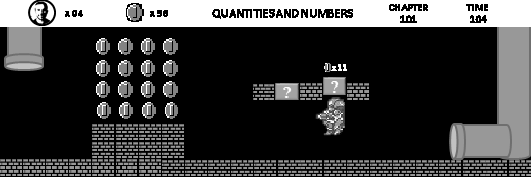
\includegraphics[width = \linewidth]{Figures/ChapterImg/Ch1.pdf}
%\end{figure}
\vfill

\newpage
\section{Thesis overview}
Standing silently in the morning haze, you wait to buy a coffee. Before you are two queues, either of which will lead to a glorious brew. But which queue contains fewer customers? Joining a queue, you look towards the coffee prices: `small' \$5, `regular' \$5.50, and `academic' \$8. Confused, you check the price again; `academic' \$6. Shrugging off the confusion of `6' and `8', you pay for your coffee and start the day. 

Often in life, we experience situations where we must compare the value of two quantities. These quantities may be physical, for example, two queues of five people, or metaphysical, for example, comparing a single queue to an internally stored representation of `ten people'. Both cases require us to perform a \textit{numerical comparison}. 

How the human brain evaluates and compares two quantities is not well understood. For example, can the brain compare two quantities at the same time? Does this process depend on the number of items in each group? How difficult is this task to complete? And does the presence of a second quantity impact our assessment of the first? Just as we perform numerical comparisons between quantities, we also perform numerical comparisons between numerals. 

When we view a numeral, for example '2', we compare its features to those of our previously stored mental representations, 1, 2, 3..., before identifying the best match. The confusion of one numeral for another reflects similarities between our mental representations. These similarities may be perceptual, for example 3 and 8 look more similar to each other than 3 and 7, or numerical, for example 1 and 2 are numerically closer than 1 and 9. But which plays a larger role in our confusions: our perception, or our internal representation of quantity?

%%AE: because the notion of similarity is tricky, as we have agreed, it'd be best to capture it in RELATIVE terms, as i have done above. I'll mention this again when we talk: be careful with the use of similarity; it is ill defined and quite contentious 


%%AE: below and else where: would either past of present tense be better than future tense? after all you have already done the work...

\subsection{Thesis aim and structure}
The aim of this thesis is to provide new insights into the fundamental cognitive processes that govern our comparisons of quantity and our confusion of numbers. This thesis is broken into two broad research streams: the comparison of quantities and the confusion of numbers. The first research stream examines how the human brain evaluates and compares two groups of items at the same time. The second research stream uses confusion data to examine the mental representations of symbolic numerals (\eg Arabic digits) and non-symbolic numerals (\eg domino tiles). 

This thesis composes eight chapters, structured into two research streams, the comparison of quantity (Chapters 2--5) and the confusion of numbers (Chapters 6--7; illustrated in Figure \ref{fig:ThesisSummary}). Chapter 1 introduces key concepts from both research streams before highlighting the aims of each subsequent chapter. Chapters 2 and 3 examine how we compare and estimate large quantities, and Chapter 4 examines how we compare small quantities. Chapter 5 will provide a theoretical extension to the previous chapters for when participants use a mixture of processing strategies. Chapters 6 and 7 examine the confusion of numbers and the dimensions along which we confuse numerals. Chapter 6 examines numeric confusions within an English speaking cohort, and Chapter 7 examines numeric confusions within a Chinese speaking cohort, before concluding with a cohort comparison. Finally, Chapter 8 will discuss the general conclusions, implications and directions of this thesis.

\begin{figure}[tbh]
\centering 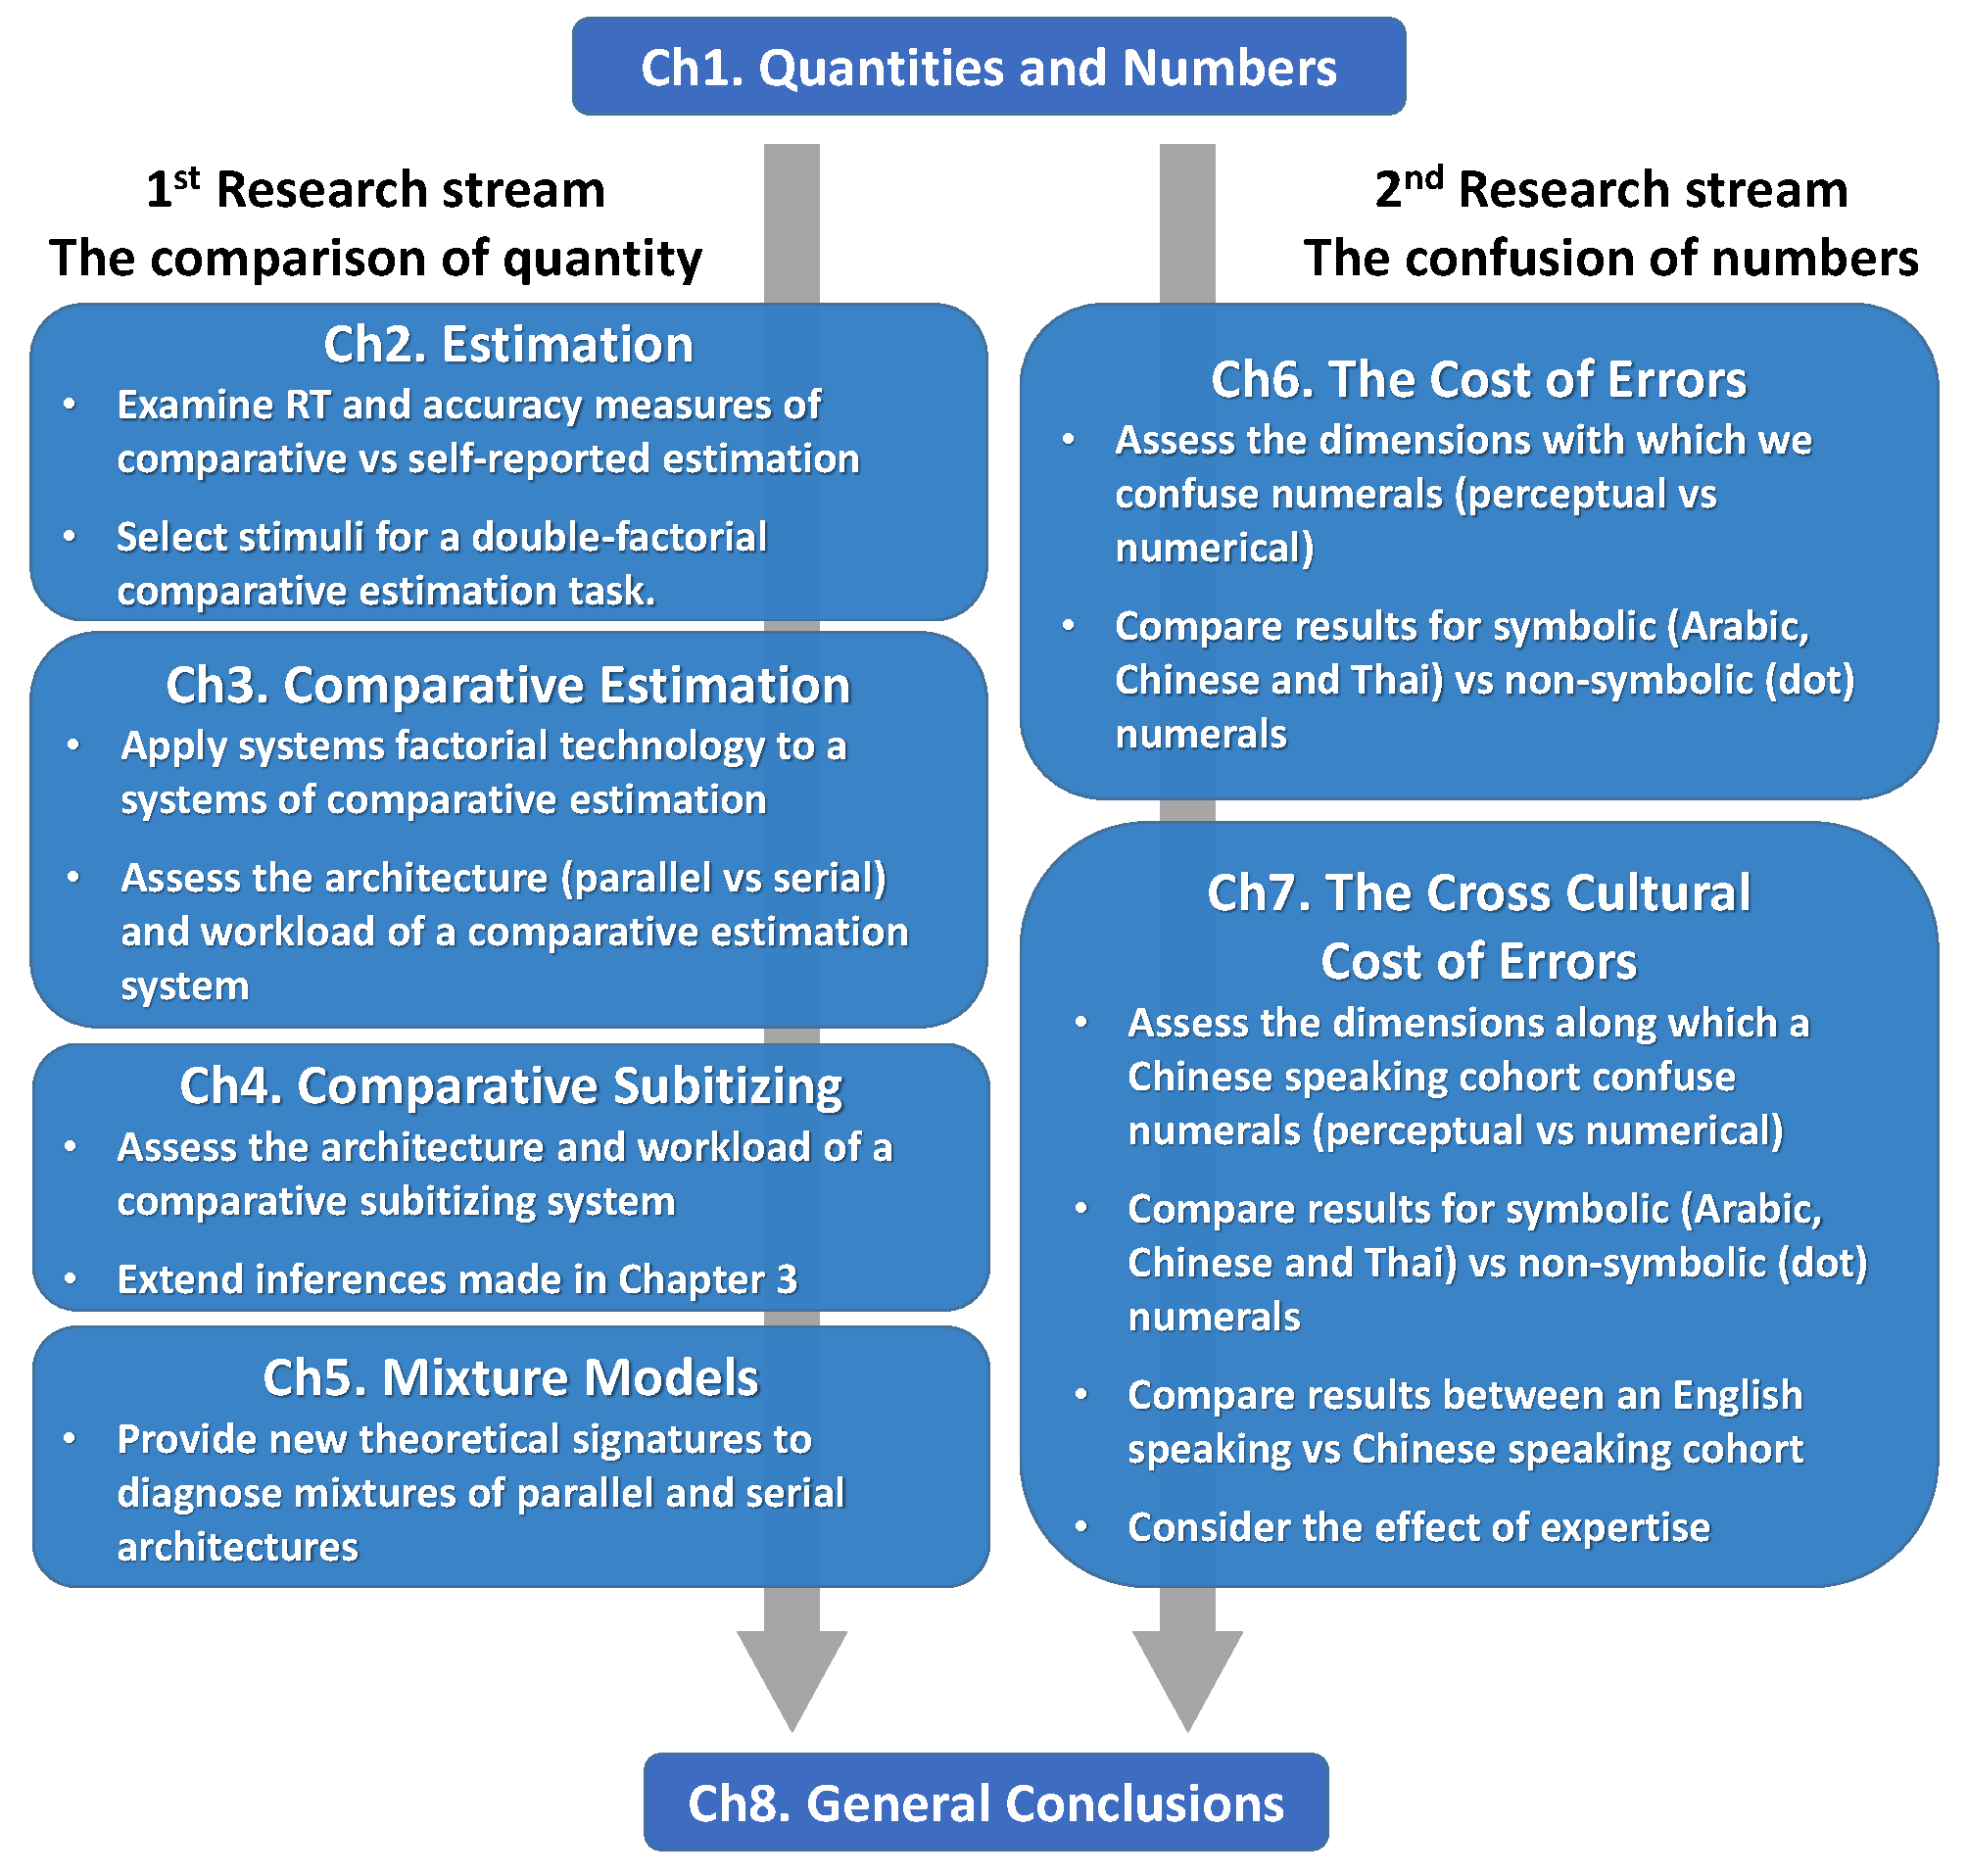
\includegraphics[width = \linewidth]{Figures/Intro/ThesisSummary.pdf}
\caption{Overview of the thesis structure. There are two separate, but related research streams: the comparison of quantity and the confusion of number. The chapters within each research stream follow directly from one another, and both streams fall under the broad umbrella of numerical comparisons.}
\label{fig:ThesisSummary}
\end{figure}


\section{Quantities and numbers}
The ability to quantify a group of numerous items and communicate their value has been critical to the development of human civilization \cite{menninger2013number}. Our collective history of trade, finance, agriculture, warfare and scientific discovery has pivoted upon our ability to quantify items and communicate number. In our modern society, we rely on quantities and numbers to measure time and distance, cook recipes, track social media engagement and perform mathematics. Although less apparent, we rely on quantities and numbers to run our computers and phones, track our money, heat our homes, and secure our electronic identities. Quantities and numbers are instrumental to our everyday lives, and as such, have been studied closely by many cognitive scientists. In the following Chapter, I summarise key concepts and findings from this literature, before expanding on the aims of each thesis chapter\footnote{For the purpose of the introduction and closing chapters, I will use the personal pronoun `I'. The pronoun `we' will be used in the content Chapters to reflect the many contributions of my collaborators.}. 

\section{Quantities}
\subsection{The enumeration of quantity}
\subsubsection{Counting}
Quantities, such as a queue of people, are assigned value through a process of \textit{enumeration}. Counting is one process of enumeration and describes the slow, sequential accumulation of items over time \cite{dehaene2011NumSense}. When we count a quantity, or \textit{item-set}, we unknowingly engaged with five basic principles of counting. 

In their investigation of children's counting, \citeA{gelmanCounting} identified the five principles that must be displayed by a countable number set. A number set must display i) a stable counting order (ordinality), ii) a one-to-one mapping between value and number, iii) cardinality, such that each number is inclusive of previous counts, iv) abstraction, so that counts may generalise to any object, and v) order irrelevance, such that the order an item is counted in does not matter. These basic principles are so complete and universal, they can be used to describe number systems across various human cultures (\eg Arabic, Chinese and Thai numerals).

The process of counting is useful when we wish to know the exact value of an item-set. For example, when we wish to detect the small difference between 14 and 15 apples, or the difference between 21 and 22 dollars. However, often we are less concerned by an exact difference between quantities, and more interested by a relative difference in magnitude. For example, quickly judging that 14 apples are fewer than 20 apples. Such judgements of quantity do not require the slow process of counting, but instead, rely on a different process of enumeration.

%% AE: paul, you use 'upon' extensively (eg rely upon), and i think it'd be good to either replace it with 'on', or at least mix a bit
% PG: Yep, I'll fix this on the read through.

\subsubsection{Estimation}
Estimation is a fast process of enumeration that characterises coarse differences in quantity by changes in relative magnitude. For example, one could estimate that a crowd of 20 people were fewer than a crowd of 30 people, however, one may not be able to estimate that a crowd of 20 were fewer than a crowd of 22. The ability to estimate changes in relative magnitude stems from our innate approximate number system (ANS). %% AE: i added coarse above, otherwise why can you tell apart 20 from 22?
% PG: Sounds great, cheers

The ANS is an inherent system presumably present in many species, including humans and primates \cite{woodruff1981primative}, parrots \cite{pepperberg2005number} and fish \cite{pepperberg2005number}. The ANS, and by extension estimation, requires very few attentional resources \cite{Burr2010} and is capable of simultaneously estimating the number of items within a scene \cite{gallistel1992ANS,dehaene2011NumSense}. This system is responsible for our ability to detect changes in relative magnitude between two quantities.

The ANS follows a logarithmic scale, obeying the Weber-Fechner law, such that detecting a difference between a small quantity and a large quantity depends on their ratio \cite{fechner1860}. For example, detecting a difference between 10 and 20 apples is approximately equivalent to detecting a difference between 20 and 40 apples.\footnote{In other words, when it comes to the ANS it's the proportional difference that `counts'.} This means small differences in quantity are often overlooked. ANS estimates balance the rapid ability to enumerate a quantity, against the inaccuracy of estimation. Although this balance is important when enumerating large quantities, it becomes unnecessary at very small counts.

\subsubsection{Subitizing}
Subitizing is the rapid and very accurate enumeration of 1--4 items \cite{kaufman1949subtizing}. Subitizing, like estimation, is able to quantify an entire item-set simultaneously; however, unlike estimation, subitizing does so without cost to accuracy. The process of subitizing was first described by \citeA[later named by Kaufman et al., 1949]{jevons1871power}\nocite{kaufman1949subtizing} who noticed five or fewer beans could be accurately and simultaneously counted, without conscious attention. The effortless nature of subitizing has led researches to speculate the process may be an innate form of enumeration.

The ability to subitize has been found in human infants \cite{fitzhugh1978role, klein1988universals} and increases from a maximum of two items, to three or four items over the ages of 2--5 \cite{starkey1995development}. The ability to subitize precedes the ability to count \cite{fitzhugh1978role} and is thought to play a role in our early ability to identify one item from a group of two or three similar items \cite{starkey1995development}. Subitizing, unlike estimation, requires attention \cite{Burr2010} and is not derived from the ANS. Rather, subitizing may be derived from the object tracking system.

The object tracking system is an innate perceptual system responsible for distinguishing one item from another and for simultaneously tracking up to four items through space \cite{feigenson2004core, pylyshyn1988tracking}. Although some have suggested subitizing is related to the ANS \cite{dehaene1994dissociable}, it is now generally considered part of this innate object tracking system \cite[but also see Revkin, Piazza, Izard, Cohen, \& Dehaene, 2008]{chesney2011evidence}\nocite{revkin2008does}. 

Subitizing, estimation and counting are three processes through which we may enumerate a single item-set. Often, we enumerate one item-set with the intention of comparing it to another. For example, we may subitize and compare the number of cookies on two plates, or estimate and compare the number of people leaving through two exists at the cinema. But how does the human brain achieve such tasks? For example, do we enumerate one group, then another, and compare them (so-called serial processing), or enumerate and compare both groups at the same time (i.e., in parallel)? 

\subsection{Comparing quantities}
We compare quantities for a variety of reasons. Sometimes we seek to directly compare and match two quantities, for example, matching guests to dinner plates. Other times, comparisons are made to answer a question of inequality, for example, which plate has more cookies? Finally, we may compare one quantity to an internal representation, for example, how many brownies will my friends eat, and will these 10 brownies be enough\footnote{At this stage, it may be apparent that this introduction was written on an empty stomach.}? The way in which we compare two quantities, for example in sequence or simultaneously, can be described in terms of the \textit{processing architecture}.

Processing architecture describes the time course at which information sources are evaluated \cite{Townsend_1995}. A \textit{serial} processing architecture finishes processing one information source (\ie quantity), before starting the next. By contrast, a \textit{parallel} processing architecture evaluates both sources of information at the same time. These descriptions of processing architecture easily extend to our comparisons of quantity.

Comparing two quantities via counting is best described by a serial processing architecture. One item-set must be sequentially enumerated (dotted arrows, Figure \ref{fig:Ch1_CountEstSub}.a), before counting may begin the next (black arrows, Figure \ref{fig:Ch1_CountEstSub}.a). Estimation and subitizing are not accumulative processes and can simultaneously enumerate a single item-set (e.g., dotted lines, Figure \ref{fig:Ch1_CountEstSub}.b). Therefore, it may be theoretically possible for two item-sets to be estimated (or subitized) and compared at the same time through a parallel processing architecture (e.g., black arrows, Figure \ref{fig:Ch1_CountEstSub}.c). Indeed, recent research indicates this might be the case. 

\begin{figure}[tbh]
\centering 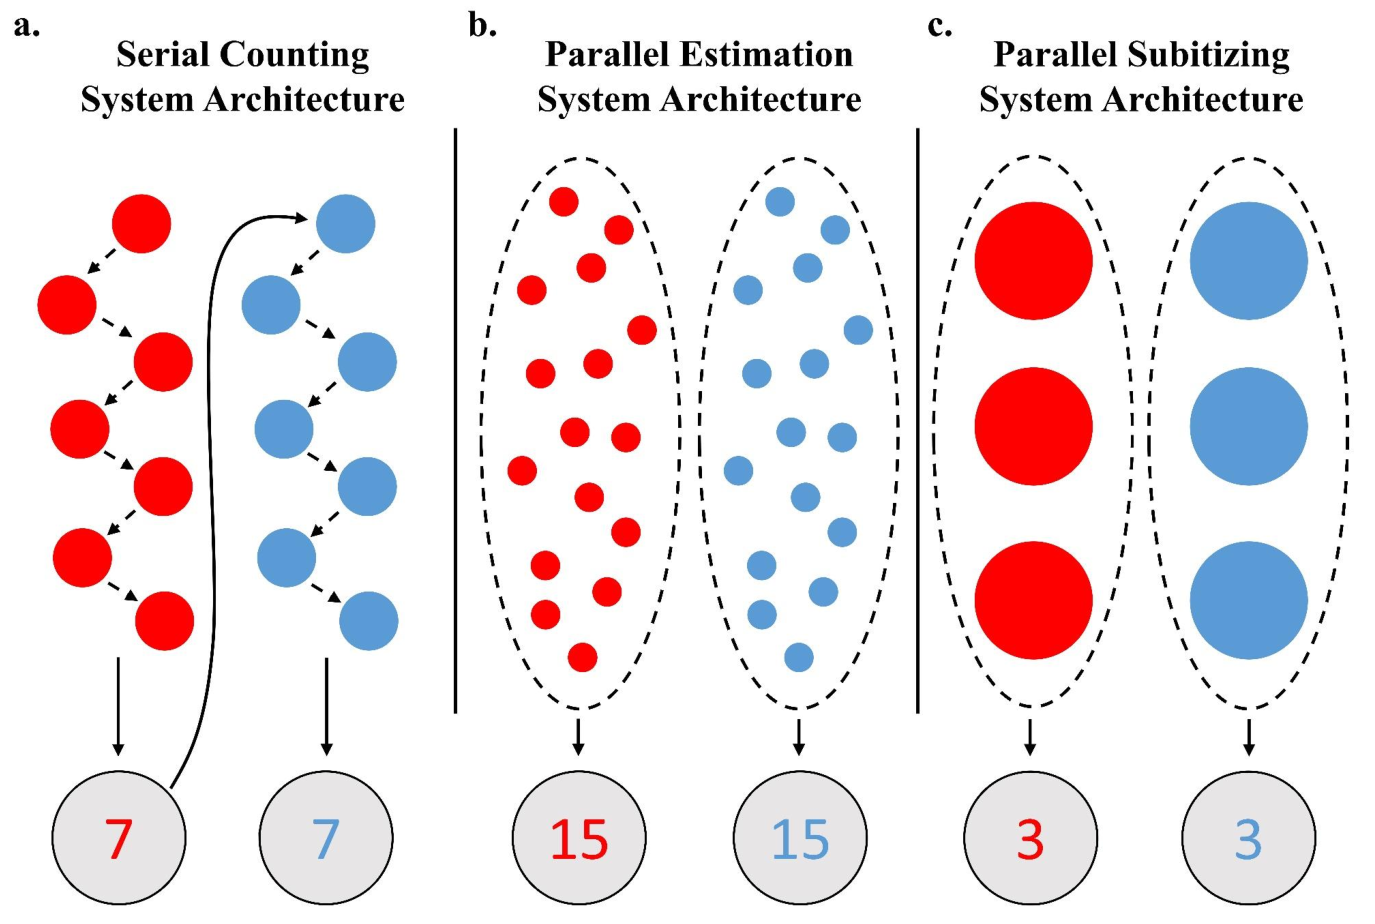
\includegraphics[scale = .65]{Figures/Intro/CountEstSub.pdf}
\caption{a) Illustration of a serial counting system architecture. Note the red-set must be counted first, before counting on the blue-set may begin. b) A theoretical parallel estimation system. c) A theoretical parallel subitizing system. Parallel systems quantify both color-sets (dashed-lines) at the same time.}
\label{fig:Ch1_CountEstSub}
\end{figure}

\subsubsection{Comparative estimation}
In their 2006 study, \citeauthor{HALBERDA_2006} provided the first evidence of a `parallel estimation system'. In this study, participants were presented an array of 1--35 dots, made from 1--6 colors. A color was probed either before or after the stimulus array and participants were asked to estimate the quantity of the probed color-set. If the probe was presented \emph{before} the stimulus array, participants had to estimate the target color-set and report the value with a number-pad. However, if the probe was presented \textit{after} the stimulus array, all color-sets had to be estimated and later, the probed color-set reported. \citeauthor{HALBERDA_2006} found estimation acuity was stable between pre- and post-probe conditions for three or fewer color-sets. Subsequently, \citeauthor{HALBERDA_2006} concluded three or fewer item-sets could be estimated at any one time through a parallel processing system. 

\citeA{HALBERDA_2006} concluded in favor of a parallel estimation system and suggested in their discussion the existence of a parallel subitizing system. As illustrated in Figure \ref{fig:Ch1_CountEstSub}.c, a parallel subitizing system would quantify two small item-sets (each item-set less than five) at the same time. Although \citeA{HALBERDA_2006} provides the first description of a parallel subitizing system for multiple item-sets, the existence a parallel subitizing system has been alluded to in other literature.

%%AE: ok here's a tricky point: parallel processing of multiple sets, as opposed to within set. I added it above and need to be careful in subsequent sections
% PG: Yep, always tricky. Thanks

\subsubsection{Comparative subitizing}
In their investigation of children's numeracy, \citeA{starkey2014groupitizing} found children could quantify an array of items faster, if the items were arranged into groups of 1--4 units. For example, an array of nine items would be enumerated faster if the array were organized into three groups of three. \citeauthor{starkey2014groupitizing} termed this process `groupitizing'. Although the cognitive architecture of groupitizing was never explored, this response-time (RT) facilitation may point towards a `parallel subitizing system'. To understand the wildly speculative nature of this claim, we must first consider a brief history of response-time modelling and the assessment of processing architecture. 

\subsection{Examining processing architecture}
Since the advent of \citeA{donders1868schnelligkeit} subtraction method, response-times have been used to make inferences about human cognition. It was \citeA{egeth1966parallel} who first used response-times to infer differences between parallel and serial processing systems. \citeauthor{egeth1966parallel} assumed that if all items within an array were processes simultaneously (\ie in parallel), the addition of further items would have no impact on decision-time. As such, a parallel system would predict a flat mean RT slope over increasing array sizes. By contrast, a serial system would predict a steep mean RT slope, increasing with arrays size. 

As an early adopter of this method, \citeA{sternberg1966high} applied these principles to examine whether short-term memory was accessed in serial or in parallel. In his task, participants were presented a list of digits followed by a probe, and were asked to report whether the probed digit was in the memory list. \citeA{sternberg1966high} found that response-times increased linearly with the length of the memory list. This `additivity' was used as evidence of a serial processing system, a claim propagated by many influential studies \cite<e.g.,>{Sternberg_1969, cohen1973hemispheric, Shiffrin1977, treisman1980feature}. However, all of these claims ignored the potential for model mimicry.

In the context of processing architectures, model mimicry describes how a slow parallel system architecture may mimic the mean response-times of a fast, serial system architecture \cite<see>[for a case study and review of this topic]{townsend2004serial}. The efficiency at which information sources are evaluated can be described in terms of workload capacity. A limited workload capacity system slows with additional sources of information (e.g., a second item-set), an unlimited workload capacity system is unaffected by additional sources of information, and a super-capacity system speeds up with additional sources of information. The mean RT predictions of \citeA{egeth1966parallel} and \citeA{sternberg1966high} only hold under the assumption of unlimited workload capacity, as a limited capacity parallel system could mimic the mean RT of an efficient serial system. To address this problem of model mimicry, James Townsend and colleagues \cite{Townsend_1995, Townsend_2004, townsend2011} have developed a theoretically driven framework and suit of mathematical tools, known as Systems Factorial Technology (SFT).

\subsection{Systems factorial technology}
SFT is a theoretical framework, augmented by experimental methodology, that uses response-time distributions to specify predictions of unique system-models. By comparing these theoretical models to experimental data, SFT is able to identify system properties without the confound of model mimicry. Specifically, SFT was designed to identify and assess the system properties of architecture, workload capacity, stopping-rule and channel (in)dependence.

Architecture describes the time-course at which information channels are combined (parallel vs serial) and workload capacity describes the system efficiency (limited, unlimited and super). Stopping-rule describes how and when processing may terminate. A self-terminating or minimum-time stopping-rule may terminate before all sources of information are fully processed (e.g., you may terminate your search for a cookie at the moment of its detection). An exhaustive or maximum-time stopping-rule must process all sources of information before a decision can be reached (e.g., you must check all the cookie's ingredients for your friend's nut allergy; see Figure \ref{fig:Ch1_ProcessingChannels}). Finally, channel (in)dependence describes whether information channels are stochastically separate. Independent channels provide no information to one-another. Dependent channels share information and may act to facilitate or inhibit the decision process \cite<see>{eidels2011}. A coactive model describes a special case of parallel processing, where information channels sum together to reach a decision (bottom panel, Figure \ref{fig:Ch1_ProcessingChannels}). Notably, a coactive model is unaffected by stopping-rule and predicts super-capacity. 

\begin{figure}[tbh]
\centering 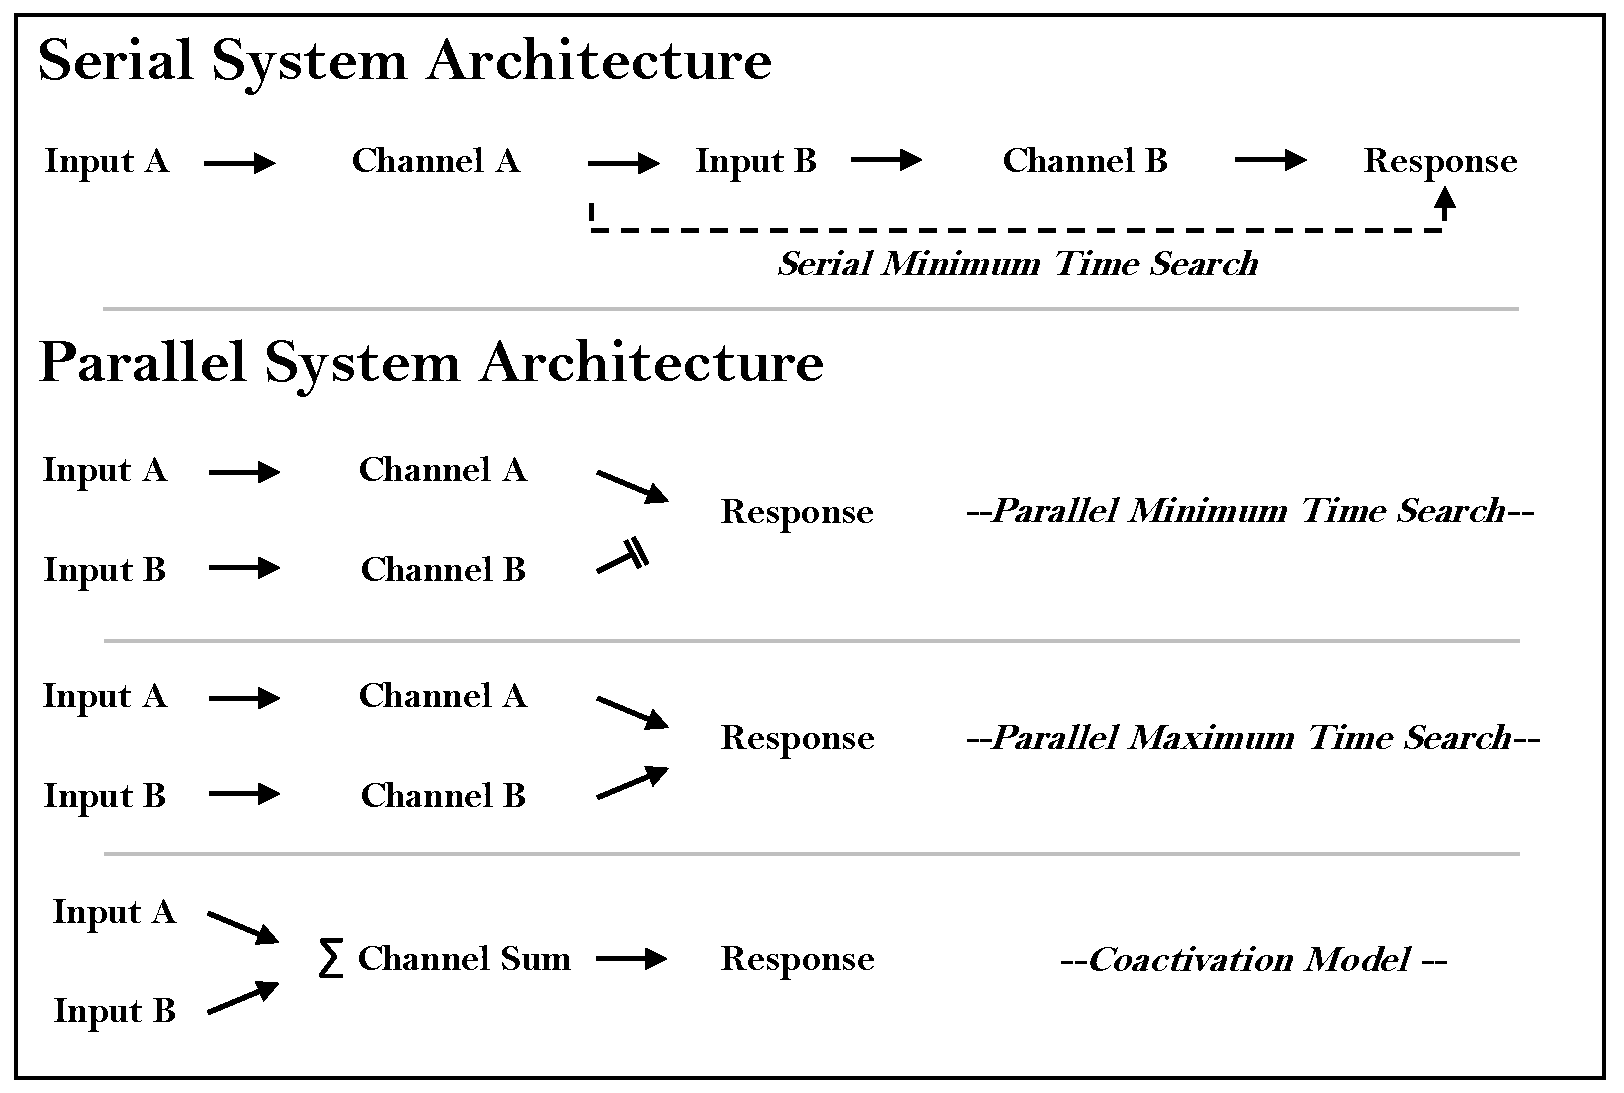
\includegraphics[scale=.54]{Figures/Intro/Architecture.pdf}
\caption{Illustration of parallel and serial processing systems, under minimum-time (self-terminating) and maximum-time (exhaustive) stopping rules. A special instances of parallel processing, coactivation, is also illustrated where channel information is summed. Coactivation models are identical under either stopping-rule.}
\label{fig:Ch1_ProcessingChannels}
\end{figure}

\subsubsection{Double factorial paradigm}
SFT is both an analysis tool set and methodological framework. SFT uses distributional analysis tools to directly assess the properties of system architecture, stopping-rule and workload capacity, under the assumption of channel independence. These analysis tools require a specific methodological design, termed the double-factorial redundant-target paradigm (DFP). Figure \ref{fig:Ch1_DFP} illustrates a prototypical DFP using a dot-detection task. Here, a target is defined by any source of light, and may appear in the left (channel A) or right (channel B) location. Load, (\ie the number of information channels), is manipulated by the presence or absence of a target. Within the target conditions exists a second manipulation of target salience, (\ie target discriminability). A high salience (H) target is easier and faster to respond to than a low salience (L) target. Double-target cells are redundant, as either target would constitute a correct `target present' response. Together, these redundant-cells host four combinations of double-target salience: high-high (HH), high-low (HL), low-high (LH) and low-low (LL). The combined manipulation of load (target presence vs absence) and salience (discriminability high vs low) allows SFT to perform independent assessments of system workload and processing architecture. 


\begin{figure}[tbh]
\centering 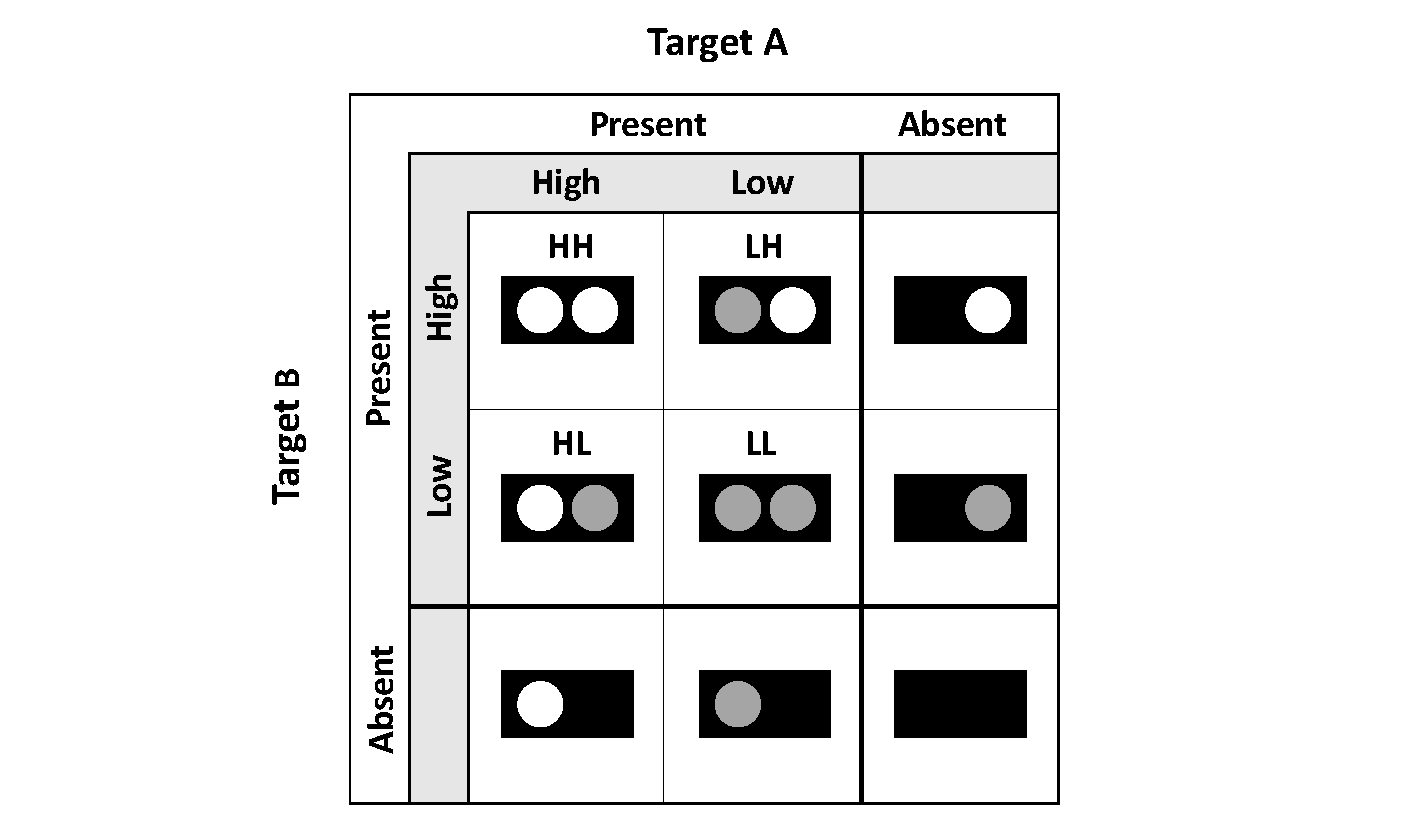
\includegraphics[scale = .6]{Figures/Intro/DFP.pdf}
\caption{Illustration of the double factorial redundant-target paradigm. A `target' is any source of light. One level manipulates workload through the presence or absence of a target. A second level manipulates target salience \ie identifiability --- high (H) or low (L). Two targets are `redundant'; either would constitute a correct target present response.}
\label{fig:Ch1_DFP}
\end{figure}

\subsubsection{Capacity coefficient}
The first factorial manipulation of load allows for calculation of the capacity coefficient [C(\textit{t})]. The capacity coefficient measures the change in efficiency of the processing system as workload, (i.e., the number of information channels), increases. The capacity coefficient is calculated by comparing the response-time distribution for double-target trials, to the response-time distribution for trials when a target is present in each channel alone --- single-target trials. Formally, the capacity coefficient is expressed as:

\begin{equation}
	\rm C(\t) = \frac{\log[S_{AB}(\t)]}{\log[S_{A}(\t)] + \log[S_{B}(\t)]}
    \label{eq:Ct}
\end{equation}

\noindent
where subscript letters refer to the processing channels when each channel operates alone, $A$ or $B$, or together $AB$. $S(t)$ refers to the survivor function\footnote{Throughout this thesis, I use the following notation: $f(t)$, for the probability density function (pdf); $F(t) = \int{f(t)dt}$ for the cumulative distribution function (cdf), and $S(t) = 1 - F(t)$ for the survivor function.} of the channel response-times; $t$ is time, and log is the natural logarithm. The measured change in efficiency between the channel conditions is evaluated against predictions derived from an unlimited capacity independent parallel (UCIP) model. Under the UCIP benchmark model, an unlimited capacity system predicts C($t$) = 1. A super capacity system, one that speeds with additional workload, predicts C($t$) $>$ 1. Finally, a limited capacity system predicts C($t$) $<$ 1. 

\sloppy{
Further predictions for the capacity coefficient have been derived under the purview of the parallel race model. Of particular interest to the current paper is the Grice lower-bound \cite{Grice1984,townsend2011}. The Grice lower-bound is a marker of performance approximately equivalent to serial processing and is formally expressed as:}

\begin{equation}
	\rm C(\t) \geq \frac{\log\{ MIN\, S_A(\t), S_B(\t)\,]\} }{ log[ S_A(\t) \cdot S_B(\t) ] }
    \label{eq:girce}
\end{equation}

\noindent
In a parallel system, violations of the Grice lower-bound suggest severely limited capacity and could be the outcome of channel dependence, where processing in one channel slows the rate of processing in the other \cite{eidels2011}. The Grice lower-bound provides a theoretical comparison by which we can compare parallel system capacity to serial system capacity. 

\subsubsection{Mean and survivor interaction contrasts}
The second factorial manipulation, that of target salience, allows for diagnosis of the system processing architecture through two measures: the mean interaction contrast and the survivor interaction contrast. The mean interaction contrast or MIC, is calculated as a double-difference of mean RT between the four factorial combinations of salience. Formally, the MIC may be written as:

\begin{equation}
	\rm MIC = \left( mRT_{LL} - mRT_{LH} \right) - \left( mRT_{HL} - mRT_{HH} \right)
    \label{eq:mic}
\end{equation}

\noindent
where $mRT$ is the mean response-time, and the subscripts denote the display salience as combinations of high (H; \ie bright dot) and low (L; \ie dull dot) double-target salience-conditions. Thus, HH indicates a trial with two salient targets (\eg two bright dots), HL and LH indicate a trial with one salient and one dull target item, and LL indicates a trial with two dull target items. As high salience targets should be responded to faster than low-salience targets, correct MIC interpretation requires the following ordering: $\rm{mRT}_{\rm HH} < mRT_{\rm HL},\, mRT_{\rm LH} < mRT_{\rm LL}$. Under the assumption of a UCIP model, and correct ordering of the mean RTs, a parallel minimum-time model predicts an over-additive MIC $>$ 0, a parallel maximum-time model predicts an under-additive MIC $<$ 0 and all serial models predict an additive MIC = 0. These three predictions allow the MIC to easily differentiate between parallel and serial models. To further diagnose stopping-rule, we must turn to the survivor interaction contrast (SIC).

The SIC is a contrast measure, similar to the MIC, but calculated from the survivor functions of each double-target salience combination. It is defined as:

\begin{equation}
	\rm SIC(\t) = \left[ S(\t)_{LL} - S(\t)_{LH} \right] - \left[ S(\t)_{HL} - S(\t)_{HH} \right]
    \label{eq:sic}
\end{equation}

\noindent
Different models predict unique SIC($t$) functions, as illustrated in Figure \ref{fig:SIC}. A necessary assumption for valid interpretation of the \SIC is the assumption of selective influence and ordering of the composite salience conditions \emph{i.e.,} $S(t)_{\rm HH} < S(t)_{\rm HL},\, S(t)_{\rm LH} < S(t)_{\rm LL}$. Fortunately, these survivor functions are easily subjected to non-parametric tests. Appropriate application of the \SIC and MIC allows for comprehensive diagnosis of system architecture and stopping rule within the double-target condition.

\begin{figure}[htb]
\centering 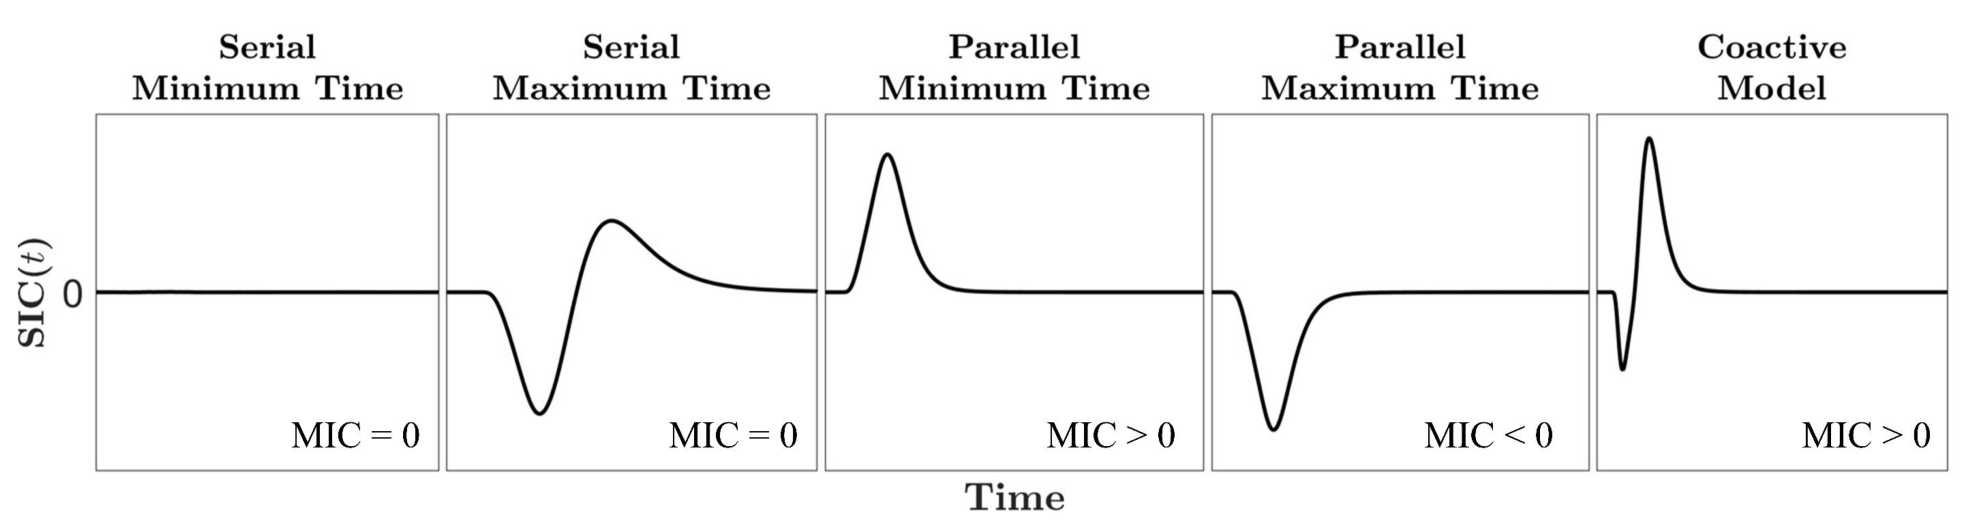
\includegraphics[scale = .47]{Figures/Intro/SIC.pdf}
\caption{Illustration of the five SIC models (and associated MIC values) predicted by the unique combinations of processing architecture and stopping rule. Note, coactivation models are identical under either stopping rule and can be identified by the combination of SIC($t$) and MIC.}
\label{fig:SIC}
\end{figure}

In summary, the distributional tools provided by SFT, once combined with the methodological framework of the double-factorial paradigm, are capable of independently assessing system workload, processing architecture and stopping-rule. This makes SFT the perfect tool-set with which to assess the workload capacity and processing architecture of i) systems of comparative estimation, and ii) systems of comparative subitizing. Now that a firm background has been established regarding SFT, system properties, system measures and comparative enumeration, I present the aims of the first research stream.



\subsection{The comparison of quantity: Chapter aims}
Thus far, I have described three processes of enumeration: counting, subitizing, and estimation, and how these processes are used to compare quantities. I have provided some evidence that two item-sets may be compared through a parallel estimation system, or a parallel subitizing system. I then detailed the issue of model mimicry and why mean RT cannot diagnose parallel and serial processing architectures without accounting for workload capacity. Finally, I described the methodological framework and analysis tools of SFT. Chapters 2--5 focus on the use of SFT and the study of comparative numerosity systems with the following aims.

In Chapter 2 I assess how participants estimate the quantity of a single item-set. The aim of this chapter was to develop a double-factorial comparative estimation task that I later test in Chapter 3. Through experimentation, I select numeric stimuli (i.e., quantities) that fit within the double-factorial framework of load and salience, required for SFT analyses. To do this, I asked participants to estimate a single item-set and report i) their estimation of quantity using a number pad, and ii) their judgement of whether the quantity was less-than a criterion. The results of this study were used to inform the selection of stimuli in Chapter 3. 

In Chapter 3 I implement a double-factorial comparative estimation task using target stimuli selected in the previous Chapter. The aim of this chapter was to assess the processing architecture and workload capacity of a comparative estimation system. To foreshadow, I find evidence of parallel processing architectures, and workload capacity that is so limited, as to be slower than a theoretical serial system. The implications and applications of these findings are discussed.

Chapter 4 extends the work of the previous chapters and develops a double-factorial comparative subitizing task. The aim of this chapter was to assess the processing architecture and workload capacity used for the comparison of small quantities. Here, I find evidence of serial processing architectures operating under severely limited workload capacity. During this chapter, I identify a handful of participants from Chapter 3 and Chapter 4 who display non-prototypical SIC signatures. These participants appear to reflect a mixture of parallel and serial processing architectures.

In Chapter 5 I provide a new set of SIC signatures by simulating and systematically varying the relative proportions of component parallel and serial processing models. These theoretical mixture model are then compared to experimental data to identify participants who displayed a mixture of processing architectures. This process was extended to illustrate the effect of mixture models on the capacity coefficient. Having covered the aims of the first research stream, the comparison of quantities, I now introduce the second research stream: the confusion of numbers.



\section{Numbers}
Quantities can be expressed in a number of ways. Historically, people have used physical markers to represent the count of an item-set, for example, a tally of ten sheep. This method is efficient for small quantities, however, becomes less-efficient and error prone at larger counts. To address this limitation, symbolic numerals were adopted by various cultures and are still used today - for example, Arabic digits. The second research stream of this thesis relates to the numerals we use to symbolically represent quantity. Where the previous research stream investigated the enumeration of an item-set, this research stream will focus on the means of numeric communication.

%%AE: i think more is needed here. Something like: "Quantities could be expressed in various ways. Historically, people used physical markers to represent the number of objects, say, a line for each cow they inteded to exchange. This method could be efficient for small quantities, but with development of commerce they arised the need to represent larger quantities. Symbolic... [say here]. Stand 1 focuses of subitising and estimation with non-symbolic representations. Strand 2 examines the use of symbolic.... 
% PG: Fixed

Human civilisations are shaped by the communication of ideas, emotions and quantities. The ability to accurately communicate quantity has been integral to the advancement of mathematics, finance, agriculture, engineering, and warfare. The importance of accurately communicating quantity has led many cultures to develop their own symbolic numeral systems. For example, the Arabic numerals 0 -- 9 and the Chinese numerals \begin{CJK}{UTF8}{gbsn} 〇 -- 九\end{CJK}. 

Often, when we view one numeral, we confuse its identify with that of another. The cost a confusion varies, and not all confusions are the same. For example, the financial cost of confusing 2 with 3 dollars, is naturally less costly than confusing 2 with 7 dollars. These confusions may be caused by perceptual similarities or numerical proximity. 

The physical similarities between two numerals, for example 2 and 7, or \begin{CJK}{UTF8}{gbsn} 二 and 三,\end{CJK} may lead us to confuse the identify of one numeral for another. The more features shared between two numerals, the higher the likelihood of a confusion. When we identify a numeral, we compare its features with those of our internal mental representations.

Mental representations are theoretical internal cognitive states thought to reflect the external world \cite{mueller2012alphabetic, eidels2016mental}. Items with more similar features are thought to be represented by closer distances within this mental space. For example, the number `2' displays a diagonal midsection and open left-face, and may be confused with the number `7'; this would suggest 2 and 7 are closely aligned along dimensions of perceptual similarity in the mental space. Although the physical properties of numerals may change across cultures, the values they represent do not.
%%AE: oh Blimey, that similarity again. Fine, leave it here [but be careful elsewhere, as i requested]

Numerals maintain the properties of cardinality (unit-value), and ordinality \cite<unique sequential ordering> {dehaene2011NumSense}. With use, these properties become embedded into our internal representation of number; our so called \emph{mental number space}. Numerals are representations of quantity and inhabit the same mental number-space as the approximate number system \cite{dehaene2011NumSense}. This makes numerals subject to basic numerical effects, such as the numerical distance effect.

In the context of numbers, the numerical distance effect describes how numerically-close numbers (e.g., 5 vs 6) are harder to compare than numbers further apart \cite<e.g., 5 vs 9>{moyer1967time}. This displays an effect of proximity between our mental representations of number and means two numerals may be confused due to their numerical proximity. But which plays a larger role in our confusion of numbers: our perceptual representations of number, or our internal representation of quantity? In Chapter 6, I aimed to address this question. 

\subsection{The confusion of numbers: Chapter aims}
In Chapter 6 I assessed the rate at which numerals were confused with one-another in an English speaking cohort. I presented participants with three symbolic numeral types (Arabic, Chinese and Thai numerals) and one non-symbolic numeral type (non-symbolic dots e.g., domino patterns), and asked participants to complete a numeral identification task. Confusion patterns were analysed using multidimensional scaling \cite{shepard1962originalMDS1, shepard1962originalMDS2, kruskal1964nonmetric}, a method used to visualize dimensions of similarity. The analysis was augmented by application of Luce's similarity choice model \cite{luce1963detection} to control for effects of response bias. We find evidence that symbolic numerals were confused (represented) by dimensions of perceptual similarity, and non-symbolic numerals were confused by dimensions of perceptual \textit{and} numerical similarity. 

Chapter 7 extends the work of Chapter 6 within a Chinese speaking cohort. In addition to assessing the dimensions by which numerals are confused, this study provides a new insight into how experience with a numeric-set changes our mental representations. The results of this study were identical to the previous chapter, except that Chinese numerals were represented differently between the Chinese-speaking and English-speaking cohort. These results are discussed in the context of expertise and its effect on our internal representations. 

Finally, Chapter 8 offers a discussion of the general findings and future directions of this research. This chapter will tie together the general conclusions of both research streams: the comparison of quantity and the confusion of number.


% Ami DONE w Intro -- 22/1/2019

\chapter{Comparative estimation} 

\label{Chapter 2}
\lhead{Chapter 2. \emph{Estimation}}
\vspace{3cm}
\newpage

% New Sections for Ami to read
% - Introduction
% - Discussion

\noindent
The method, results and discussion of this Chapter appear as Appendix A of the published manuscript `comparative estimation systems perform under severely limited capacity' \cite{garrett2019comparative}. I would like to acknowledge the work of Laura A. Waters and Alexander Thorpe, in assisting with data collection for this thesis chapter. 

\color{\Red}
\section{Chapter aims}
In this Chapter, we aimed to develop a new experimental design that merges a comparative estimation task with the double-factorial paradigm --- a requirement of SFT. The double-factorial paradigm, as designed by Townsend \citeyear{Townsend_1995}, requires two levels of manipulation: load and salience. The manipulation of load is manifested by factorial manipulation of signal x presence, such that there are typically four resulting conditions: target-signal A present, B present, both present, or none. A second manipulation of salience --- nested within the manipulation of load --- must selectively influence the discriminability of the target, making high-salience targets easier and faster to respond to than low-salience targets. In addition to these `standard' requirements of the double-factorial paradigm, our novel design must engage the approximate number system in order to answer fundamental questions regarding systems of comparative estimation (as applied in Chapter 3). We begin with a brief introduction on how estimation tasks and the approximate number system are typically measured, before showcasing a novel experimental procedure designed to address the aims of this chapter.

\section{Assessments of estimation}
Estimation acuity is typically assessed through the self-report method. Participants are presented a range of item-set sizes and using a number-pad, report their estimates of quantity. The self-report method has three advantages: the task is simple, reliable, and may help establish if the approximate number system is being engaged \cite{Whalen1999, Cordes2001}.

Establishing ANS engagement is critical to any future assessment of comparative estimation systems. When we compare two quantities, we may i) estimate the quantity of each item-set, or ii) compare low-level perceptual covariates of quantity, such as area or density, to inform our decisions \cite{dehaene2011NumSense}. Since density and area are covariates of quantity, this strategy may lead to an accurate response while not engaging the ANS. For the purposes of assessing systems of comparative estimation, we must ensure estimates are performed using the ANS and not low-level perceptual covariates of quantity. 

One method of measuring ANS engagement is through the self-reported coefficient of variance. As previously noted, the ANS follows a logarithmic scale. When the ANS is engaged in a self-reported estimation-task, the mean and standard-deviation of response-estimates increase in a linear fashion with the number of items to be enumerated. This results in a coefficient of variance (standard-deviation divided by the mean) ranging from approximately 0.14 to 0.4 \cite<see>{Whalen1999, Cordes2001, HALBERDA_2006}. This method provides a measure of ANS engagement, but at a cost to the fidelity of estimation response-time.

% AE: perhaps say in a sentence above how the coefficient of variance is calculated ?
% PG: Done

When a participant self-reports a numerical estimate, it is unclear at what time the cognitive processes behind their decision terminated. For example, does a decision terminate when a participant finishes typing their estimate? Or does a decision terminate when the participant begins typing their estimate? Might a participant change their decision as they are typing, and how does this factor into the response-time? While self-reported estimates are useful for assessing ANS engagement, this method provides a poor assessment of ANS decision time. This is a problem for the primary tools of SFT --- the SIC and capacity coefficient --- that rely on response-time distributions. The self-reported method has a further limitation, in that it cannot conform to the binary `yes' and `no', target-present vs target-absent response-set necessary for SFT. To address these limitations, we consider an alternative numerical task.

\subsection{The comparative numerosity task}
An alternative method for assessing response-times using a binary response-set while potentially engaging the ANS, is a comparative numerosity task \cite{leibovich2014comparing,pansky2002comparative,piazza2004}. Here, subjects are asked whether an item-set is greater-than or less-than a specified criterion, to which a binary `yes' or `no' response is provided. In this response-format, decision-time and response-time are tied to a single key-press, creating a more reliable measure of decision finishing-time. Furthermore, the comparative numerosity task is designed to engage and measure a specific aspect of the number system: the numerical distance effect \cite{buckley1974comparisons}. 

Under the numerical distance effect, item-sets that are closer together are harder to relatively estimate than item-sets that are further apart \emph{i.e}., estimating whether 22 items are greater-than 20 items is harder than estimating whether 30 items are greater-than 20 items \cite{moyer1967time}. As such, closer item-sets incur a reliable penalty to response-time and accuracy. This makes the numerical distance effect a useful manipulation of difficulty (salience), in a task that requires a stable manipulation of response-time, such as SFT. The next challenge is in merging this comparative numerosity task with the necessary double-factorial paradigm used in SFT. 

\subsection{The double-factorial numerosity task}
The comparative numerosity task can be modified to meet the requirements of the double-factorial paradigm (see Figure \ref{fig:EgIllus}.a as an example). Target item-sets can be defined as being less-than a specified criterion, creating a binary `target-present' vs `target-absent' manipulation of load (for example, Figure \ref{fig:EgIllus}.b)\footnote{Typically, a greater-than criterion is used in comparative numerosity task \cite{piazza2004,price2012,libertus2016, leibovich2014comparing,pansky2002comparative} as it aligns with the size- and semantic-congruency effects; however, as the reader will soon find, a less-than criterion works equally well and becomes necessary in Chapter 4 when comparing smaller quantities, (i.e., subitizing).}. A double-target trial would be two item-sets, both less-than the criterion. Each `channel' or item-set, could be identified by set-color, for example, red or blue discs (see Figure \ref{fig:EgIllus}.c). Target salience can be manipulated by the numerical distance effect with target quantities close to the criterion incurring a reliable cost to response-time, relative to quantities that are further away. This task design meets the requirements of the double-factorial paradigm, yet, introduces a new complication: the target-absent channel.

\begin{figure}[hbt]
\centering 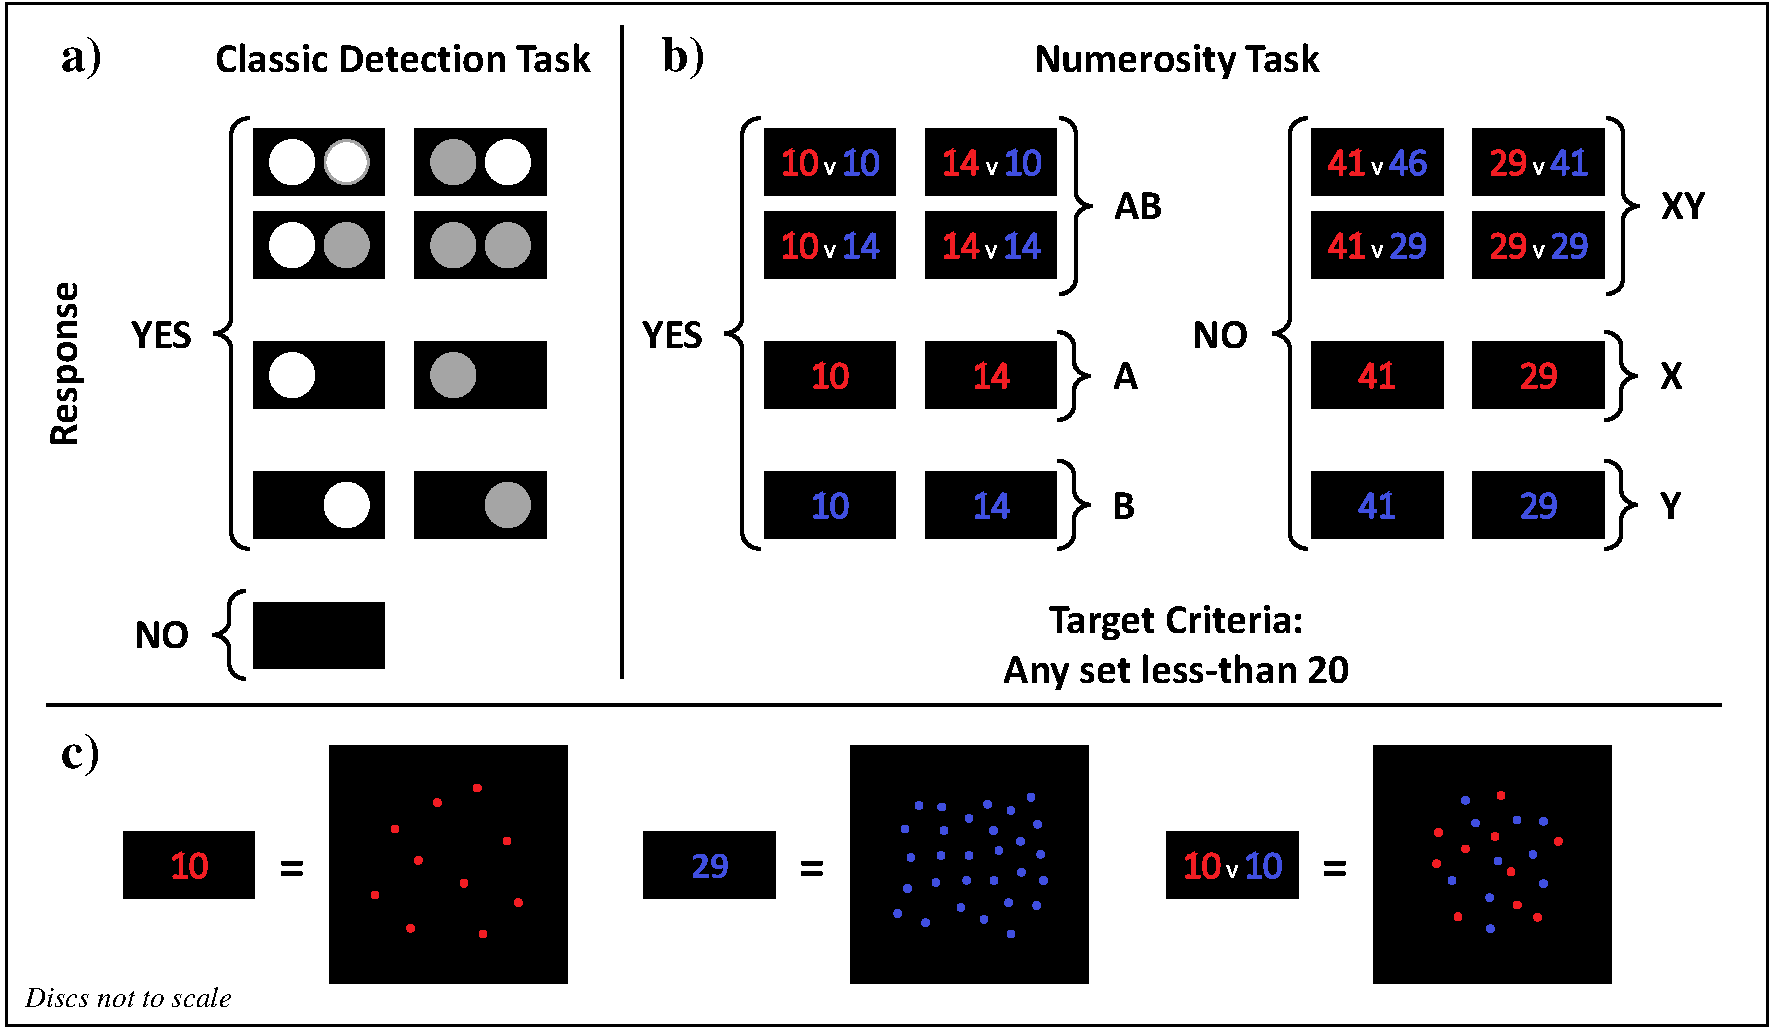
\includegraphics[width=\linewidth]{Figures/Estimation/ExampleIllustration.pdf}
\caption{Illustration of a) stimuli and correct responses for the classic `OR' detection task (Townsend \& Nozawa, 1995), b) colored digits symbolizing example quantities for the proposed double-factorial numerosity task, c) illustrative example of what these symbolic values would look like. A, B and AB refer to single-target and double-target trials; X, Y and XY refer to single-distractor (target-absent) and double-distractor trials.}
\label{fig:EgIllus}
\end{figure}


% AE: i think the above section needs a CONCRETE illustration and can be aided by an exmaple figure of th estimuli used
% PG: Done.

The classical \citeA{Townsend_1995} double-factorial design (Figure \ref{fig:EgIllus}.a) was created as a detection task, however, this design is not applicable to estimation. In our task, participants must encode the quantity of a stimulus and not terminate their response via stimulus detection. \citeauthor{eidels2010stroop} encountered a similar issue enforcing the semantic processing of word stimuli. To encourage stimulus encoding, \citeauthor{eidels2010stroop} introduced distractor stimuli.

In the context of a less-than comparative numerosity task, a distractor stimuli would be any quantity greater than the criterion. For example, given a criterion of 20, a quantity of 14 would be a target and a quantity of 29 would be a distractor (see Figure \ref{fig:EgIllus}.b, right). Note, the term `distractor' here is specific to the SFT literature; the stimulus need not distract the participant, but rather enforce full encoding of the target item. Following the methodology of \citeauthor[(but see also, Little, Eidels, Fifić \& Wang, 2018\nocite{Little2018_CCF})]{eidels2010stroop}, the salience of the distractor quantities may be manipulated in a similar fashion to the target quantities. This would produce high- and low-salience target and distractor stimulus sets.

The distributional response-time tools of SFT --- the SIC and capacity coefficient --- rely on a large number of high-accuracy trials, with a significant response-time difference between high- and low-salience conditions. As such, target and distractor salience levels must meet two criteria within the double-factorial design. There must be a significant effect of response-time between high- and low-salience conditions and response accuracy should be high (\ie $\geq$90\%) at both levels of salience. 

\section{The current study}
So far in this Chapter, we have described how a comparative estimation task, implemented in a double-factorial design must i) engage the ANS, ii) use a comparative numerosity task, iii) use both target and distractor quantities, and iv) produce a significant response-time effect between the levels of salience while maintaining high response accuracy. The remainder of this Chapter will be dedicated to two experiments, specifically designed to address these requirements. 

In the current study, participants viewed a single item-set entirely composed of either red or blue discs. Participants completed two separate tasks -- a self-reported estimation task and criterion judgement task (a precursor to the comparative estimation task). In the self-report task, participants freely reported their estimates of quantity with a number pad. In the criterion judgement task, participants judged whether a presented item-set was less-than a criterion of 20 items. ANS engagement was established using the coefficient of variance as measured by the self-reported estimation task. The numerical distance effect --- our measure of salience --- and response accuracy were assessed relative to the criterion in the criterion judgement task. ANS engagement was inferred for the criterion judgement task by comparing results to the self-report task. In both tasks, quantities ranged from 10--46. This meant items were presented both above and below the central criterion of 20 items in the criterion judgement task. Together, these tasks ensured ANS engagement, assessed how numerical distance affected response-times and accuracy within the range of estimation, and provided an informed selection of high- and low-salience stimuli for the double-factorial design applied in Chapter 3.

\color{black}

\section{Method}
\subsection{Participants}
Participants were 20 undergraduate students ($F$ = 16) from the University of Newcastle. Participants were reimbursed two course credits over a one hour testing session. Participants reported as not being color blind, and as having normal or corrected-to-normal vision. The mean age was 24.4 years ($SD$ = 9.09).

\subsection{Stimuli and apparatus}
Testing was conducted in the Newcastle Cognition Laboratory. Stimuli were presented on a 21.5inch Dell S2240L (60Hz) monitor. Stimuli were generated on a Dell Optiplex 7040 computer using python 2.7.14 and the Pygame 1.9.2b package. Responses were made using a standard `qwerty' keyboard.

Stimuli comprise a single set of uniformly sized, non-overlapping discs. The item-set (disc) color was either entirely red or blue. Each disc was located randomly within a central circular field of view. At a viewing distance of 60 cm, each disc subtended a visual angle of 0.14 degrees (0.15 cm), while the circular field of view subtended a visual angle of 9.52 degrees (10 cm). Stimuli were presented on a black background. Red and blue color sets were matched for value and chroma using the Munsell color scheme \cite{Cochrane2014}, and varied only by hue. Contrast and brightness effects were further controlled using a GLoptic spectis 1.0 photometer. Red and blue colors had RGB values of [241, 29, 34] and [64, 79, 223] respectively. 

Stimulus set-sizes were logarithmically spaced to reflect the approximate number system. Item sets contained either 10, 11, 12, 13, 14, 16, 18, 22, 24, 27, 30, 33, 37, 41 or 46 discs. In the criterion judgement task, target item-sets comprised less-than 20 items and non-target item-sets comprised greater-than 20 items. This resulted in seven target and eight non-target item-sets within this task type, all within the range of estimation. 

\subsection{Procedure}
Each participant completed two within-subject response tasks, a self-reported estimation task and a criterion judgment task, over one 60 min experimental session. During the self-report task, participants used the number pad to report their estimate for the total number of discs presented on a given trial, before pressing the enter key to end the trial. During the criterion judgment task participants reported the presence of a target item-set --- those containing fewer than 20 discs --- with the `z' key, and the presence of non-target item-sets --- those containing more than 20 discs --- with the `/' key. Task order and response-keys were counter balanced between participants.

Participants completed a practice block and five experimental blocks for each task. Each block contained 60 trials, with the probability of presenting each item-set equated within a block. Accuracy feedback, `correct' or `incorrect', was displayed at the end of each practice trial within the criterion task. The true item-set numerosity was displayed at the end of each practice trial during the self-report task. Feedback was not provided during experimental blocks. Each participant completed 300 self-report experimental trials and 300 criterion judgment experimental trials. 

The progression of a trial was the same regardless of the experimental task. On a trial, participants viewed a central fixation cross for 500 ms (0.28 x 0.28 degrees visual angle) followed by a 500 ms blank. Then, participants viewed a stimulus item-set for 1000 ms followed by a backwards mask for 500 ms. Participants had 10,000 ms to respond from the onset of the stimulus. The blank screen inter stimulus interval (ISI) was 500 ms.

\subsection{Data Analysis}
Differences between conditions of set-size were assessed at the group level. Participants were excluded if accuracy in the comparative judgment task was less than 90\% in either the highest (46) or lowest (10) set-size conditions. In the self-report task, trials were excluded from analysis if the time-difference between the first numeric key-press and the enter-key exceeded 2 standard-deviations of the mean. This method removed excessively long responses where subjects may have changed their decision after starting their response. During the criterion-response task, trials that exceeded $\pm$2SD of the mean response-time were excluded. Mean RT differences between set-sizes in the comparative judgment task were assessed using paired sample \textit{t}-tests, calculated in Matlab 2015b.

\section{Results}
\subsection{Self-report task}
One participant was excluded from the analysis of both tasks due to accuracy being less-than 90\% in the largest set-size condition of the comparative judgment task. The mean and standard-deviation of self-reported response-estimates are presented in Figure \ref{fig:Ch2_ANScoefVar}. In line with expectations from the approximate number system, subjects displayed a log-linear increase in both the mean and standard-deviation of response-estimates with a coefficient of variance equal to 0.18. This coefficient of variance falls within the range predicted when the ANS is engaged.

\begin{figure}[htb]
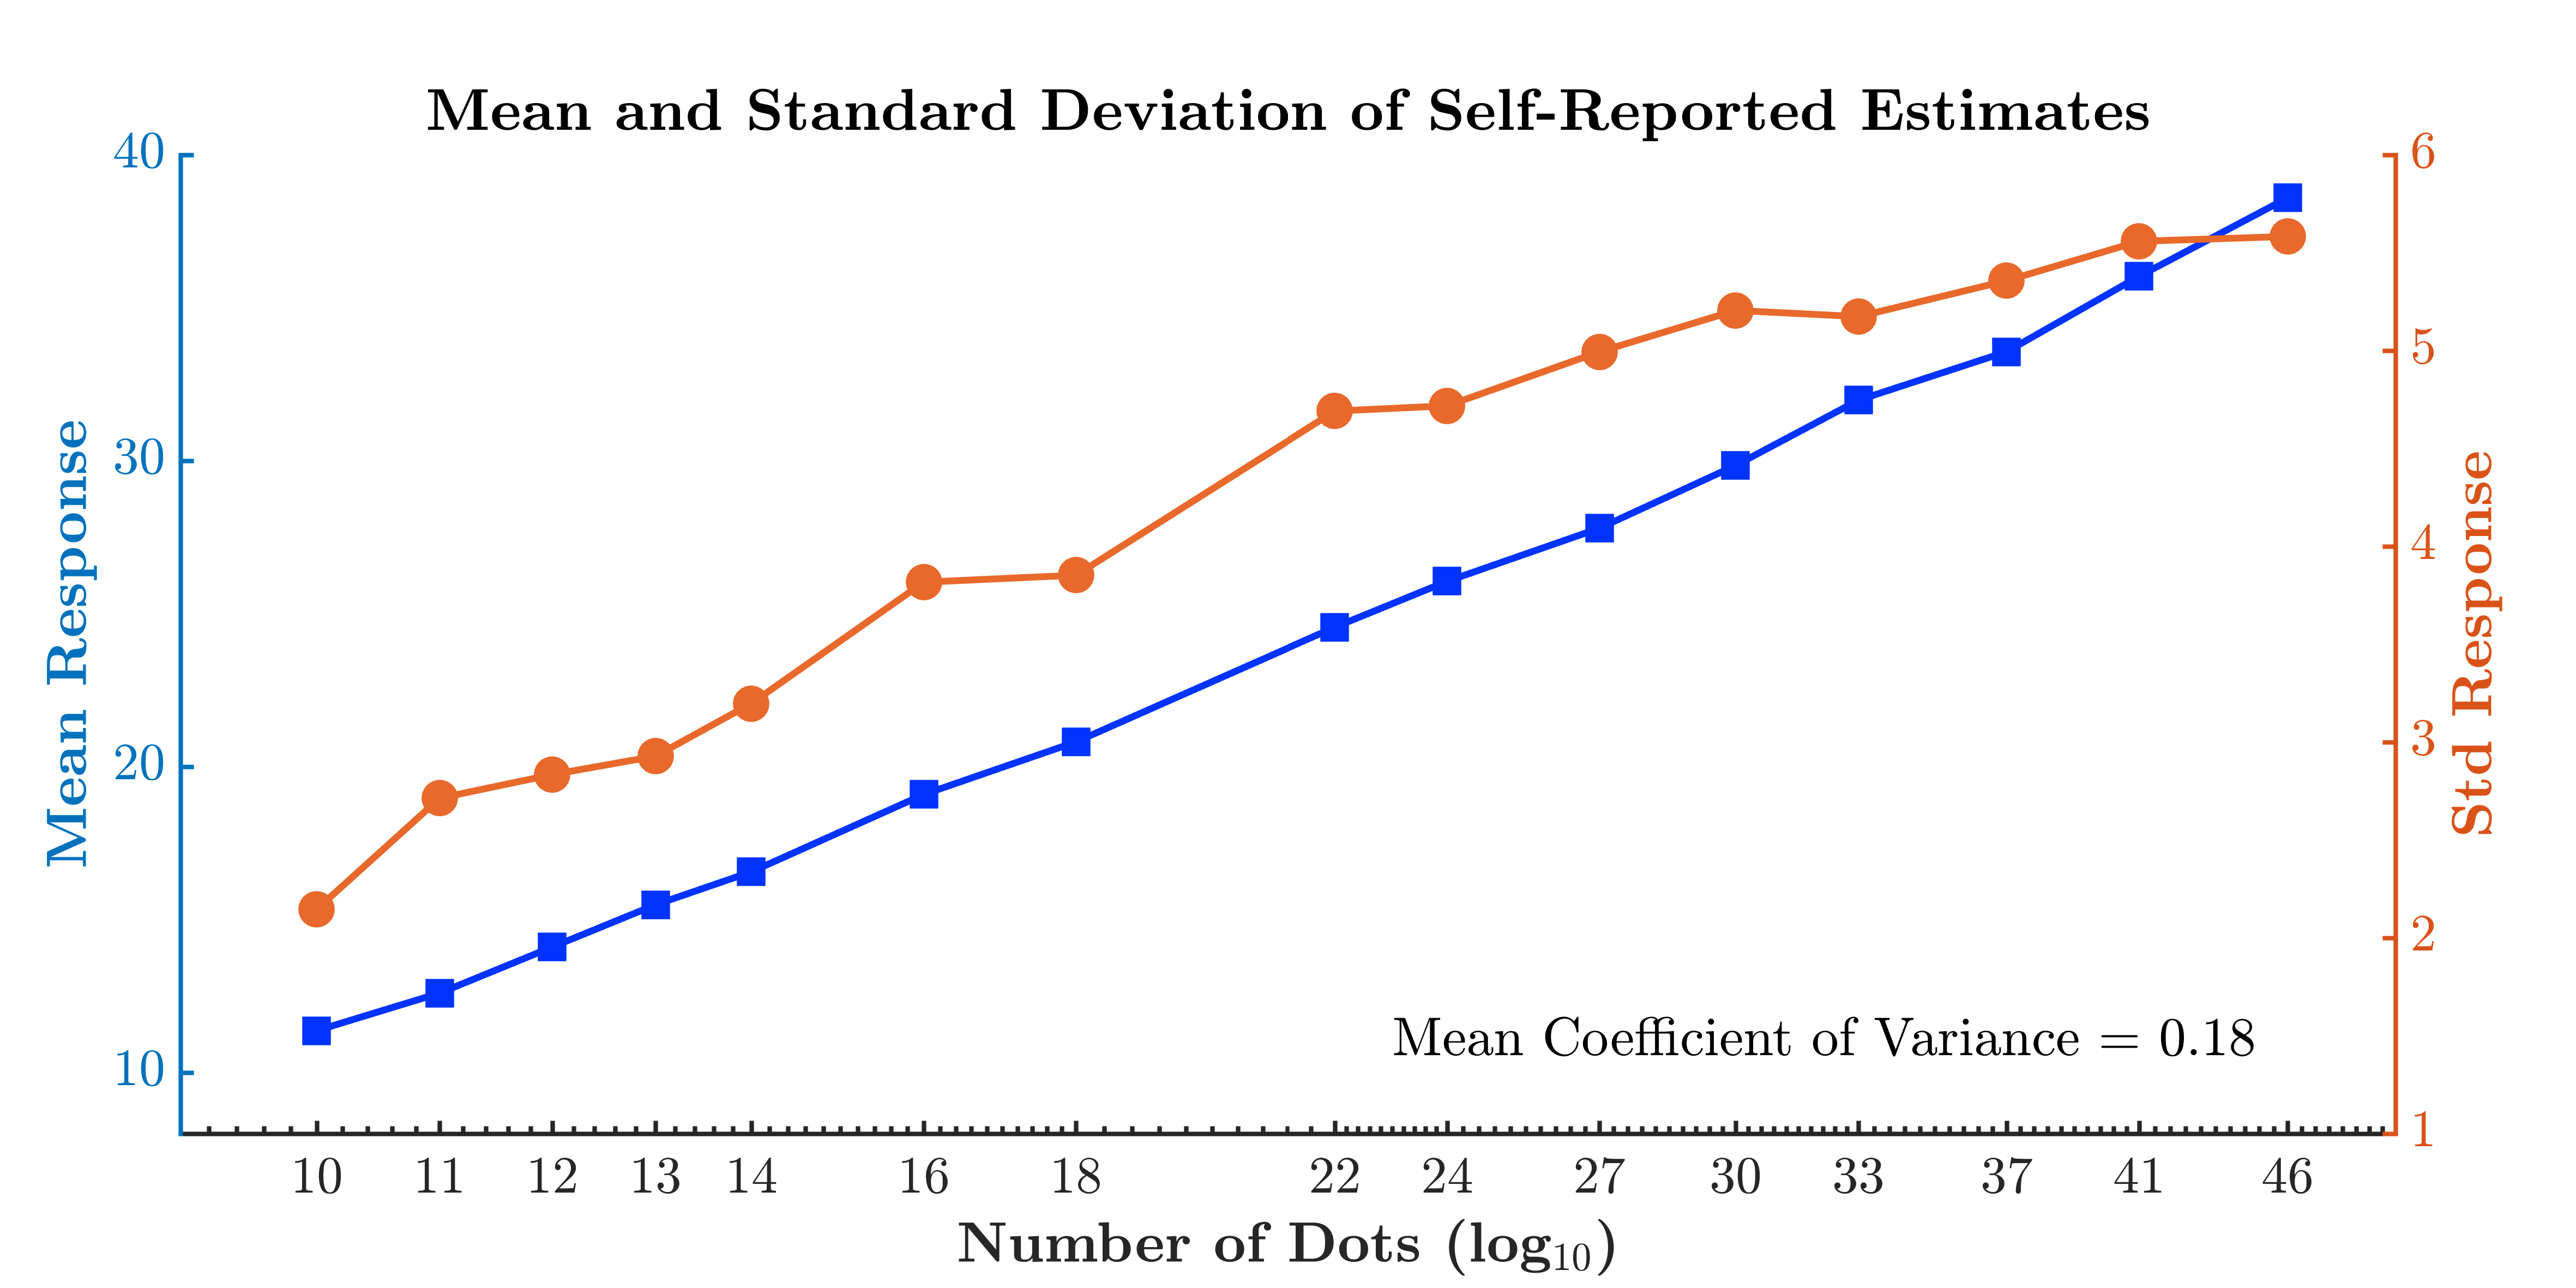
\includegraphics[scale=.4]{Figures/Estimation/CoefVar.png}
\caption{Mean (blue) and standard-deviation (orange) of self-reported response-estimates across set sizes 10--46 plotted on a log$_{10}$ scale. The mean and standard-deviation of response-estimates increase in a log-linear fashion with set-size. The mean coefficient of variance was equal to 0.18 and ranged between 0.15--0.22. This log-linear increase in the mean and standard-deviation of estimates, and a coefficient of variance falling between 0.14 and 0.4, aligns with predictions of the approximate number system.}
\label{fig:Ch2_ANScoefVar}
\end{figure}

% AE: would it be worth to plot in this figure a dotted line that marks perfect calibration (ie, where response = stimulus) to let the reader see the calibration, or lack of ?
% The Figure becomes a bit messy when I do this and it's not critical to the interpretation.

\subsection{Comparative judgment task}
At the group level, accuracy was highest at set-sizes 10 ($M$ = .98, $SD$ = .09) and 46 ($M$ = .99, $SD$ = .06), and decreased to the lowest accuracy at set-size 22 ($M$ = .59, $SD$ = .38; see top panel in Figure \ref{fig:CritVsExact}). Likewise, mean RT was fastest at set-sizes 10 ($M$ = 520 ms, $SD$ = 80 ms) and 46 ($M$ = 514 ms, $SD$ = 78 ms), and peaked at set-size 22 ($M$ = 760 ms, $SD$ = 180 ms; see middle panel in Figure \ref{fig:CritVsExact}). Both accuracy and response-time trends support the presence of a numerical distance effect, with estimation becoming less accurate and slower for item-sets closer to the criteria of 20. No speed-accuracy trade off was observed between item-sets. 

\begin{figure}[hbt]
\centering 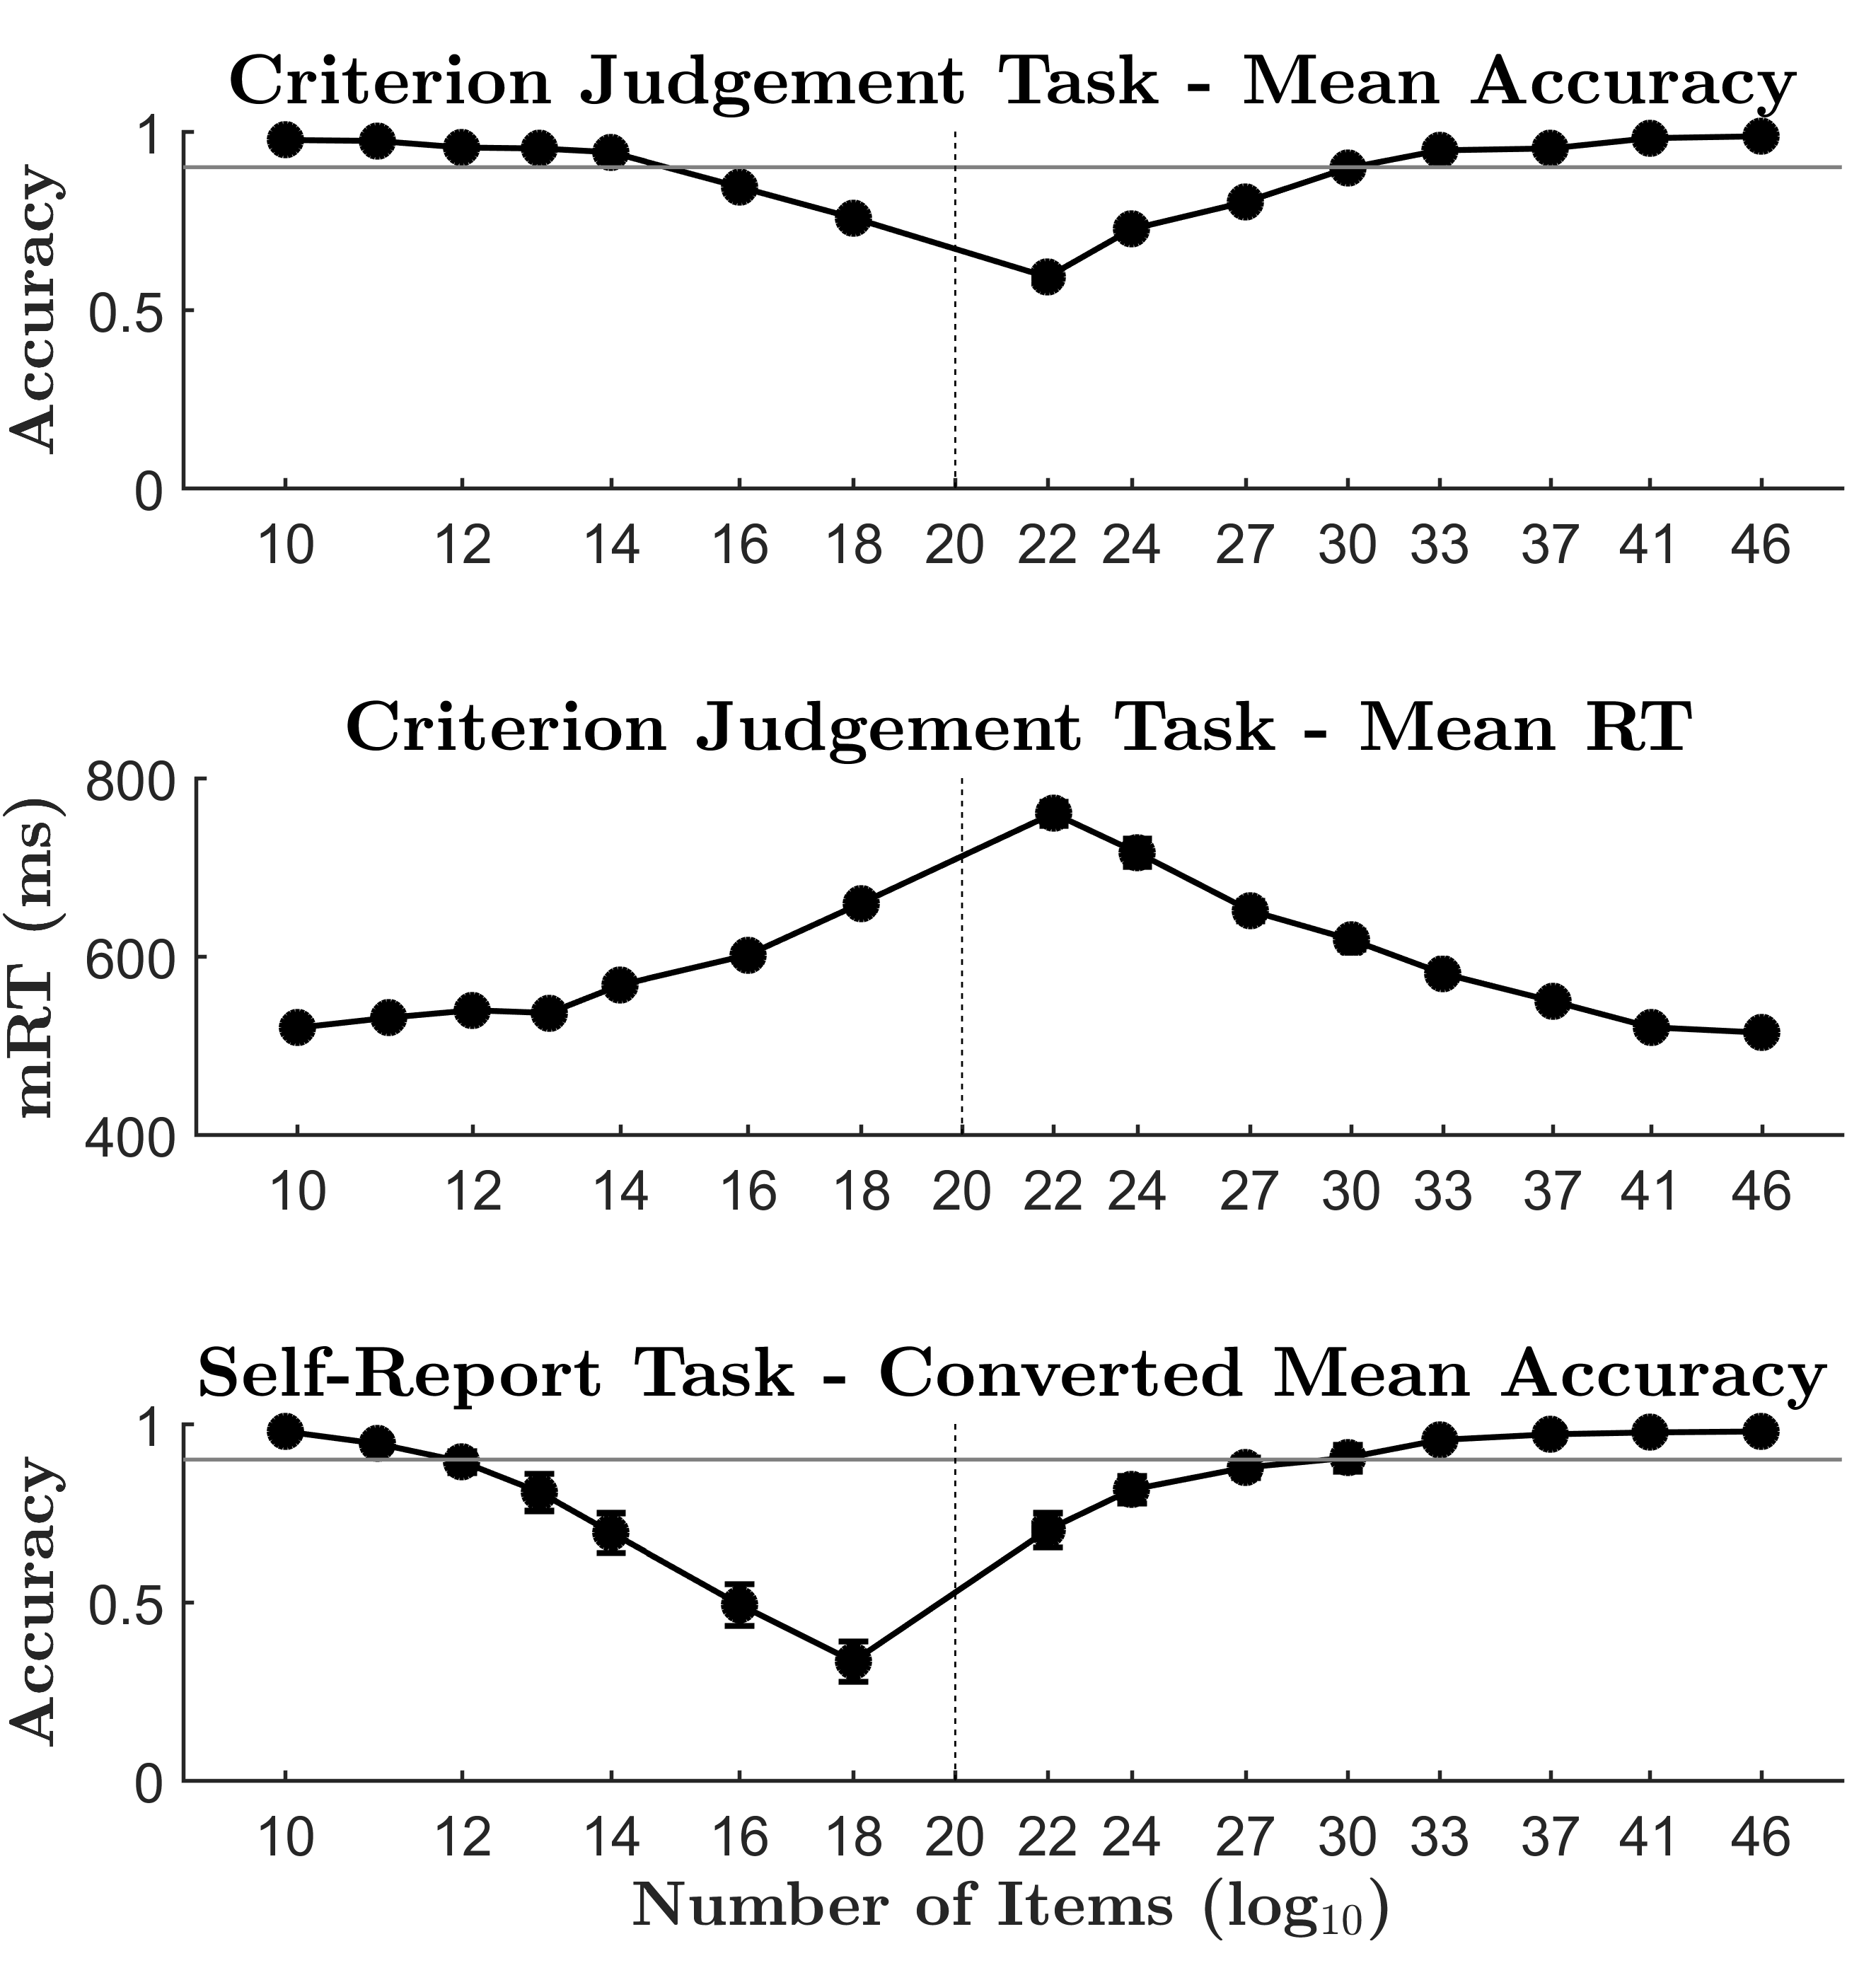
\includegraphics[scale = .75]{Figures/Estimation/FIG15JPG.png}
\caption{Mean accuracy (top) and mean response times (middle) for all participants across set sizes 10-46 in the criterion response-task, and converted mean accuracy (bottom) across set sizes 10-46 for the self-report task. The dotted line represents the response criterion of 20 and the solid horizontal line in accuracy plots illustrates the 90\% threshold. Item set-size is logarithmically spaced along the x-axis. Error bars show $\pm$ one standard error of the mean.}
\label{fig:CritVsExact}
\end{figure}

\subsection{Self-report accuracy vs comparative judgment accuracy}
To compare accuracy between tasks and determine if the ANS was engaged in both tasks, we transformed the self-reported estimates into accuracy scores based on the comparative numerosity task. Correct responses were those that accurately reported the stimulus as either less-than or greater-than 20. These transformed mean accuracy results are displayed in bottom panel of Figure \ref{fig:CritVsExact}. This panel illustrates a trend in accordance with the numerical distance effect. Accuracy is highest at set-sizes 10 ($M$ = 0.98, $SD$ = 0.01) and 46 ($M$ = 0.98, $SD$ = 0.01) and lowest at set-size 18 ($M$ = .33, $SD$ = 0.06). 

On average, accuracy was higher in the criterion judgment task ($M$ = 0.89, $SD$ = 0.12) when compared to the converted-accuracy of the self-report task ($M$ = 0.82, $SD$ = 0.15; $t$(18) = -3.233, $p$ $<$ 0.01). Both tasks illustrate a clear numerical distance effect on accuracy, an effect mirrored by response-time in the criterion judgment task. These trends suggest the numerical distance effect was engaged within both the self-report and criterion-judgment tasks and support the notion that the ANS was engaged in both tasks. 

\subsection{Selection of salience levels}
One purpose of the current experiments was to select high- and low-salience stimulus levels for a double-factorial comparative estimation task. This requires the selection of a high-salience and low-salience target ($<$ 20), and a high-salience and low-salience distractor ($>$ 20). Salience levels were selected based on three criteria. i) Stimulus accuracy must equal or exceed 90\% accuracy, ii) there must be a significant response-time effect between high- and low-salience conditions, and iii) target and distractor salience levels must be separated by the same Weber-fraction. Separating salience levels by the same Weber-fraction should theoretically produce similar numerical distance effects between target salience levels and distractor salience levels.

\subsubsection{Target salience levels}
For target responses ($<$ 20) within the criterion judgment task, accuracy was $\geq$90\% for item-sets 14, 13, 12, 11 and 10 (see the 90\% horizontal line across accuracy plots in Figure \ref{fig:CritVsExact}). Of these item-sets, the 14 item-set is closest to the criteria of 20 and experiences the slowest response-time (see Figure \ref{fig:CritVsExact}). This is in line with the predictions of the numerical distance effect. The 14 item-set differs to the 20 item-set criteria by a Weber fraction of 0.7. Application of this Weber fraction to the 14 item-set returns an equivalent proportional difference of 10 items. Paired samples \textit{t}-test analysis of the group mean response-times revealed a significant difference between set-sizes 14 (\rt{568}{136}) and 10 (\rt{520}{80}; \tval{18}{-4.54}{$<$ .001}). This significant numerical distance effect indicates that the 14 item-set and 10 item-set conditions would be appropriate for the low salience (\ie slow response; 14 item-set) and high salience (\ie fast response; 10 item-set) target conditions within a double-factorial paradigm. 

\subsubsection{Distractor salience levels}
For non-target or distractor responses ($>$ 20), accuracy in the criterion judgment task was $\geq$90\% for item-sets 30, 33, 37, 41 and 46. Given a Weber fraction of 0.7, a low-salience distractor would contain 29 items and a high-salience distractor would contain 41 items. As accuracy was in excess of 90\% for an item-set of 30 items, we accepted 29 items as our low-salience distractor.

Paired samples $t$-test analysis of group mean response-times revealed a significant difference between set-sizes of 30 (\rt{619}{141}) and 41 (\rt{520}{84}; \tval{18}{37.686}{$<$ .01}). This indicates there would be significant response-time difference between our selected levels of low-salience (29 item) and high-salience (41 item) distractors. As these conditions meet our requirements of accuracy and response-time, and adhered to the same Weber-fraction as our target stimuli, we accepted 29 and 41 items as our distractor item-sets for the upcoming double-factorial design.

\color{\Red}
\section{Discussion}
When asked to view a single set of red (alternatively blue) discs, participants were shown to estimate the quantity of items with similar accuracy, by either self-reporting the quantity on a number pad, or by comparing the quantity to a central criterion. The coefficient of variance for self-reported estimates was within the range expected if the ANS was engaged. In the comparative judgment task, a numerical distance effect was observed for both accuracy and mean RT. The distance effect was also observed in the accuracy of the self-reported estimates. Comparable accuracy trends suggest the ANS may have been engaged in both task types. Target and distractor salience levels (item-sets of 10, 14, 29 and 41 discs, to-be compared against a fixed criterion of 20) were selected using data from the criterion judgment task. These levels will be used in the double-factorial design of Chapter 4, when we investigate systems of comparative estimation.

\subsection{ANS engagement}
Estimates made in the self-report task appear to have engaged the ANS. The coefficient of variance fell within the range predicted when the ANS is engaged. This finding is necessary, but not sufficient to prove ANS engagement. In a similar fashion, the numerical distance effect observed in both tasks is necessary, but not sufficient to prove ANS engagement. However, having met these burdens of evidence, and having established similar effects of accuracy in both task types, we speculate that the ANS was engaged in both the self-report and criterion judgement tasks. In Chapter 3, we will expand on this work by developing a double-factorial comparative numerosity task that, based on these experiments, should also engaged the ANS. 

% AE: why is it critical to assume ANS was engaged? as you point out the evidence is weak (necessary but sufficient), so why commit to it?

\subsection{Over vs under-estimation}
Mean accuracy displayed different patterns of over- and under-estimation between tasks. Converted mean accuracy in the self-report task displayed patterns of over-estimation. Conversely, comparative judgments displayed patterns of under-estimation. 

The difference in over and under estimation between task types might reflect a difference in task designs. The comparative judgment task used a singular point of comparison (20 items), where the self-report task allowed free responding and a post-hoc imaginary point of comparison. If the act of comparing items to a criterion resulted in the underestimation of quantity, this effect would be absent in the self-reported data. Determining whether the change from under- to over-estimation is due to the change in task design would require further experimental testing. We leave this as an avenue of future research. 

\subsection{Conclusion}
In this Chapter, participants were asked to freely report their estimates of quantity using a number pad, or compare their estimates of quantity to a pre-determined central criterion. In both tasks, participants appeared to engage their innate approximate number system and displayed clear numerical distance effects for both accuracy and response-time. High and low salience stimuli (item-sets 10, 14, 29 and 41) were selected using these numerical distance effects, and will be applied in the following double-factorial comparative numerosity task. These item sets displayed high accuracy, significant effects of response-time between high and low-levels of salience, and a consistent Weber-fraction of 0.7. The findings of this Chapter are informative for how we estimate a single item-set, however, provide no insight into how we estimate and compare two quantities. In the following Chapter, we will apply these findings to develop a double-factorial comparative numerosity task and apply SFT to address fundamental questions regarding systems of comparative estimation.
\color{black}

% AE: "participants appeared to engage their innate approximate number system "  >>> WHY is it so important to note we engage ANS  


% Paul 2 Ami: I tried to add the 20 item elbow in, but it doesn't actually explain anything about the findings in the data.
%A second account that may explain a shift from over to under estimation may be the interaction between task type and the change in self-reported estimates for items greater than 20. It has long been established that self-reported estimates of quantity are very accurate for items within the range of subitizing ($\leq$ 4) and become increasing less-accurate above this range, producing a response-accuracy `elbow' \cite<see>{kaufman1949subtizing}. In a very recent investigation, \citeA{portley2019second} established a second elbow within the range of estimation for items above and below 20. For quantities above 20, self-reported estimates become increasingly compressed relative to quantities below 20. Although it is likely this finding applied to our self-reported estimates of quantity, it 


% Ami DONE w Chapter 2 -- 29/10/19
\chapter{Systems of estimation} 

\label{Chapter 3}

\lhead{Chapter 3. \emph{Estimation systems}}
\vspace{3cm}
\newpage

% This is pretty much the paper we submitted
% I don't think there is anything added that you
% need to read. If anything, things have been 
% removed to fill Chapters 2 and 4. 

\noindent
The method, results and discussion of this Chapter appear in the published manuscript `comparative estimation systems perform under severely limited capacity' \cite{garrett2019comparative}.

\section{Chapter overview}
Often in life we need to enumerate or evaluate the number of items in some set to address fundamental questions concerning quantity. For example, how many tomatoes do I have in my shopping bag and would that be enough for tonight's salad? Some enumeration decisions require us to compare two large quantities to some internal representation or criterion. For example, a soccer referee must ensure that each side has exactly 11 players. Conveniently, the teams are clearly marked by their shirt color -- red or blue. But somewhat inconveniently, the teams are physically separated for only a short period of time, then the whistle blows and the teams intermix. When item-sets, (e.g., football teams), intermix, the estimation of each item-set may become harder. But could this added difficulty have any effect on \emph{how} a cognitive processing system estimates two item-sets? 

Previous work \cite{HALBERDA_2006} has found up to three item-sets may be estimated at the same time, through a parallel estimation system. But does this system hold when we estimate two quantities and compare them to an internal criterion, or instead, do we need to sequentially compare each item-set? Finally, how efficient are these systems and what cognitive mechanisms inhibit their function?

In this Chapter, we will characterize information-processing approaches for the estimation of two colored item-sets (red and blue discs), when comparing these sets to an internal representation of quantity, (e.g., 20 items). To accomplish this, we will apply the findings of Chapter \ref{Chapter 2}, and test a comparative estimation task in the style of a double-factorial paradigm. Using experimental data, we will apply the mathematical tools of SFT to a comparative estimation task and highlight differences in individual's estimation-systems when (i) two item-sets are intermixed and (ii) when two item-sets are physically separated. 

The primary aims of this Chapter are to i) determine the processing architecture of a comparative estimation systems, ii) assess this workload capacity of this system, and iii) consider the applications and constrains of a parallel estimation system when item-sets are mixed vs separated. Additionally, we will assess whether low-level covariates of quantity, such as area, facilitate or inhibit the estimation-system. We will begin with a brief summary of important concepts and literature, before applying the findings of Chapter 2 to a double-factorial comparative estimation task. 

\section{The estimation of quantity}
The number of items within a single set (say, number of blue team members) may be estimated through the approximate number system (ANS). This system is inherent to many species \cite{woodruff1981primative,pepperberg2005number,agrillo2008fish,dehaene2011NumSense}, and is capable of simultaneously estimating the number of items within a scene \cite{gallistel1992ANS,dehaene2011NumSense}. ANS estimates differ from the exact process of counting and rely on changes in magnitude to detect differences in quantity \cite{gallistel1992ANS}. This allows the ANS to make rapid representations of quantity, balanced against the inaccuracy of estimation. 

The ANS follows a logarithmic scale, obeying the Weber-Fechner law, such that detecting a difference between a small quantity and a large quantity depends on their ratio \cite{fechner1860}. For example, detecting a difference between 10 and 20 players is approximately equivalent to detecting a difference between 20 and 40 players. This relationship results in a distinct linear increase in the mean and standard-deviation of response-estimates as a function of their ratio, (i.e., coefficient of variance; see Chapter 2). The detection of differences in magnitude is a key aspect of the ANS and has led researchers to an important task design: the comparative numerosity task.

In a comparative numerosity task, participants are briefly presented with two sets of items, and are asked to decide which item-set has a larger quantity \cite{piazza2004,price2012,libertus2016, leibovich2014comparing,pansky2002comparative}. Typical findings reveal item-sets that are closer in numerosity, for example, 20 and 25, are less accurate and slower to estimate than item-sets that are further apart, for example, 20 and 30. This phenomenon is known as the numerical distance effect. In Chapter 2, we substantiated the numerical distance effect and inferred ANS engagement using a self-reported estimation task and a criterion judgement task. Although a numerical distance effect is a hallmark of the ANS, informed comparisons of quantity can be made without the use of the ANS.

When presented with two item-sets, an informed comparison of quantity may be made by comparing low-level perceptual covariates of quantity. For example, it is possible to identify the larger of two item-sets by comparing the total item-set luminosity, brightness or area \cite{HALBERDA_2006}. Studies of comparative numerosity will typically complete multiple experiments, independently controlling for each of these factors \cite{inglis2014}, thereby ensuring any effect is a result of the ANS and not due to these perceptual covariates of quantity. Although these stringent designs excel at measuring the acuity of comparative judgments, they systematically ignore the much deeper question, $how$ does the cognitive system estimate two sources of information at the same time?

\section{Comparative estimation systems}
\citeauthor{HALBERDA_2006} (2006) aimed to answer this question by presenting participants with an array of 1-35 dots, made from one to six colors. Participants were presented with colored probes, either before or after the stimulus onset, and had to estimate and type the number of items in the probed set. Accuracy was stable for estimates of three or fewer item-sets, for both the probe-before and probe-after conditions. Subsequently, \citeauthor{HALBERDA_2006} concluded three or fewer item-sets may be estimated at any one time through a parallel estimation-system. Their novel experiment was the first to assay the parallel processing architecture that underlies the estimation-system for multiple item-sets. However, the study did not measure a second key system property, workload capacity. 

Workload capacity is a measure of information-processing efficiency that assesses how the rate of processing changes in response to an increase in load, for example, another item-set to estimate. In \citeauthor{HALBERDA_2006}'s study there is an implicit assumption that the addition of further item-sets would not change the rate of estimation in what is called an unlimited capacity process. This is a reasonable assumption in the context of a single item-set. Estimation response-time has been shown to increase log-linearly with item set-size \cite{Whalen1999}, and to require very few attentional resources \cite{Burr2010}. This could suggest that the estimation of a single item-set is an unlimited capacity process and that multiple item-sets may be estimated in a similar manner. However, more recent work using the diffusion model has challenged this assumption. 

\citeA{park2015} applied the drift diffusion model \cite{ratcliff1978Diffusion} to estimates of quantity and simultaneously assessed estimation speed and acuity. Participants viewed two item-sets and decided which set contained more items. By modeling both accuracy and RT, Park and Starns found a speed-accuracy trade off when estimating set-sizes of different ratios. This suggests people may need to manage limited resources in an effort to maintain the speed of processing while using the ANS (with unlimited resources, participants could have responded both quickly and accurately without the need to trade-off between speed and accuracy). Understanding the capacity of a system is a crucial part of diagnosing how information sources are combined. This is because a difference in system's capacity may fully explain mean RT predictions otherwise accounted for by the system processing architecture.

As we covered in Chapter 1, processing architecture describes how information is combined from multiple sources and is generally categorized as either parallel or serial. A parallel system processes information from multiple sources simultaneously. A serial system must complete the processing on one information source, before it initiates the processing of another. Previously, parallel and serial systems have been identified through patterns in mean response-times. However, due to the phenomenon of model mimicry \cite{Townsend1971, Townsend1972, TOWNSEND_1983} --- where the mean RT of a slow, limited capacity parallel system my mimic the mean RT of a more efficient serial system --- alternative methods for diagnosing parallel and serial systems have since been developed.

Systems Factorial Technology or SFT, is a set of tools developed by James Townsend and his colleagues to overcome issues of model mimicry by directly measuring system capacity and processing architecture. SFT has been applied to a range of studies involving visual perception, such as binocular dot presentations \cite{Townsend_1995}, facial feature identification \cite{Wenger2001, Wenger2006}, visual search tasks in the presence of distractors \cite{Fific2008}, and even the number-size congruency effect \cite{fitousi2018system}. 

In Chapter 1, we covered the requisite methodology of SFT --- the double-factorial design, and in Chapter 2 developed numeric stimuli to fit within this framework. As we noted in the second chapter, SFT was originally intended for perceptual discrimination tasks. For example, was a dot of light presented in location A or location B? Following the methodology of \citeA{eidels2010stroop}, the current study utilized distractor stimuli (item-sets greater-than 20) to encourage participants to engage in the estimation of the target item-sets (quantities less-than 20). As highlighted by \citeA{eidels2010stroop}, the introduction of distractor items alters the factorial combinations of load and allows for the calculation of additional system measures \cite{little2015resilience, Little2018_CCF}.

\section{The extended double-factorial design}
Under the classical double-factorial design, the first factorial level manipulates workload by the presence or absence of a target. This produces single-target (A), single-target (B), double-target (AB) and no-target conditions (see Chapter 1, Figure \ref{fig:Ch1_DFP}). The log ratio of the survivor processing times for the double-target, as compared to the single-target conditions, provides a measure of workload capacity: the capacity coefficient (see Chapter 1, equation \ref{eq:Ct}). The introduction of distractor stimuli alters this first level of workload and introduces the conflict-target conditions.

Conflict-target conditions describe those instances where a target (A or B) is displayed in the presence of a distractor (X or Y). The inclusion of distractor stimuli expands our conditions of load to include double-target (AB), double-distractor (XY) and conflict-target (AY or XB) conditions. The inclusion of distractor stimuli within the double-factorial design is termed the \emph{extended double-factorial design}. Just as in real life, important `target' information is often displayed in the presence of distractors. For this reason, a new tool was recently added to the SFT analysis suite, the \emph{Resilience Difference Function} \cite{little2015resilience}.

\subsection{The resilience difference function}
In their investigation of workload capacity, \citeauthor{little2015resilience} \citeyear{little2015resilience} noted that the presence of distracting channel information inflated the response-times for conflict-target trials, where a target and a distractor are both present, relative to single-target trials, where a target is presented in isolation. As such, substituting single-target trials with conflict-target trials in the calculation of the capacity coefficient would lead to an inflated estimates of C($t$). This meant a new measure of workload capacity needed to be established.

\citeauthor{little2015resilience} developed the resilience functions to eliminate the influence of distracting information in the calculation of processing architecture and workload capacity. The resilience functions are calculated under the assumption that the rate of processing in the target channel is fixed, (i.e., target-salience values are either high or low). Additionally, separate resilience functions are calculated for conditions with high distractor salience (R$_{high}$($t$); equation \ref{eq:Rhigh}), and low distractor salience (R$_{low}$($t$); equation \ref{eq:Rlow}). The difference between R$_{high}$($t$) and R$_{low}$($t$) functions provide a non-biased estimate of workload in the presence of distractors (equation \ref{eq:Rdiff}), which we employ in the current investigation. The resilience functions are defined as: 

\begin{equation}
	\rm R_{high}(\t) = \frac{-\log[S_{AB}(\t)] }{ -log[ S_{AY_H}(\t) \cdot S_{X_HB}(\t) ] }
    \label{eq:Rhigh}
\end{equation}

\begin{equation}
    \rm R_{low}(\t) = \frac{-\log[S_{AB}(\t)] }{ -log[ S_{AY_L}(\t) \cdot S_{X_LB}(\t) ] }
    \label{eq:Rlow}
\end{equation}

\begin{equation}
	\rm R_{diff}(\t) =  R_{high}(\t) - R_{low}(\t)
	\label{eq:Rdiff}
\end{equation}

\noindent where AY and XB represent conditions where a target (A or B) is displayed in one channel, and a distractor (Y or X) is displayed in the other. Like other SFT measures R$_{diff}$($t$) is a useful diagnostic measure because different models predict different functional forms, as illustrated in Figure \ref{fig:Rd}.

\begin{figure}[htb]
\centering 
\includegraphics[scale = .37]{Figures/EstSystems/FIG3JPG.png}
\caption{Illustration of five unique R$_{diff}$($t$) functions predicted by the unique combinations of processing architecture and stopping rule. Parallel minimum-time models predict R$_{diff}$($t$) = 0 (left panel), serial minimum-time, serial maximum-time and parallel maximum-time models predict R$_{diff}$($t$) $<$ 0 (with variations to slope and degree; middle panels), and coactive models predict R$_{diff}$($t$) $>$ 0 (right panel).}
\label{fig:Rd}
\end{figure}
\color{black}

The extended double-factorial design and associated resilience functions provide system measures of target processing in the presence of distracting information. 

\subsection{Perceptual covariates of quantity}
A key concern in designing any comparative numerosity task is the impact of low-level perceptual covariates, such as area and density. For example, consider the task of choosing the fewer of two item-sets within a fixed perceptual field. If the size of each item were fixed, the area of each item-set would provide information regarding the smallest quantity (\ie that item-set with the least area). Similarly, the density of each item-set would also provide numerical insight (\ie smaller quantities, on average, would be less dense within a fixed field of view). 

Low-level perceptual covariates may be used to successfully make comparative judgments of quantity, without engaging the ANS. If not controlled for, our system measures the MIC, SIC, capacity coefficient and resilience functions, may inadvertently assess processing times for the perceptual system, instead of the estimation system. 

To address the potential confound of perceptual covariates, studies of comparative numerosity often complete a series of independent experiments. Each experiment is designed to independently control for one numerical covariate, for example item-set area \cite{HALBERDA_2006}. In line with these studies, we aim to control for the primary numerical covariate --- item-set area --- in our assessment of estimation systems. Ideally, we would complete a full investigation into the other covariates of quantity, such as brightness, density and luminosity. However, our task design will already be quite complex, in so far as it addresses a second issue: item-set separability.

\subsection{Item-set separability}
When item-sets are grouped by distinct perceptual features \eg color or orientation, they are easier to identify \cite{treisman1980feature} and estimate \cite{Burr2010,HALBERDA_2006}. When item-sets intermix, \eg red and blue players on a field, the quantity of each item-group may become harder to discriminate. This change in difficulty may be accompanied by a change in processing architecture \ie parallel to serial, or, a change in workload capacity \ie unlimited to limited. As such, it is important to assess system properties when item-sets are intermixed, and physically separated. Furthermore, we must also give thought to the way in which item-sets are separated, and the effect this may have on estimation system properties. 

Performance on a range of visual processing tasks, has been shown to improve when information is split bilaterally across the left and right visual hemifields \cite{alvarez2005independent,delvenne2005capacity,kraft2013visual}. It is thought each hemifield can access independent pools of workload capacity and thereby facilitate visual processing \cite{alvarez2005independent}. This bilateral advantage extends to processes of enumeration; predominantly subitizing, but potentially estimation \cite{pryor2015bilateral,delvenne2011bilateral}. 

The current study is concerned with how we enumerate everyday item-sets; not item-sets independently processed by separate hemifields. In theory, the bilateral field advantage could improve the workload capacity of an estimation system. However, this is unlikely to occur when comparing everyday quantities. To remove this confound from the current study, we will present item-sets as either i) intermix, or, ii) separated by a horizontal meridian. By presenting item-sets as vertically aligned, any confound posed by the bilateral field advantage should be removed \cite{delvenne2011bilateral}. 

\section{The current study}
In the current study, participants were presented with two colored item-sets (red and blue discs) and were asked to decide if either set contained less-than 20 items. Workload was assessed by comparing double-target processing times to single-target processing times. Conflict-target workload was assessed via the resilience difference functions. Finally, processing architecture, whether items were assessed in parallel or serial, was assessed with the SIC and MIC via the manipulation of target salience. 

Target and distractor sets were presented at both high and low levels of salience, as selected in Chapter 2. Due to the numerical distance effect, high salience items were further from the criterion of 20 than low salience items. High salience targets consisted of 10 discs, and low salience targets of 14 discs. High salience distractors consisted of 41 discs, and low salience distractors of 29 discs. This manipulation of target salience allowed for the assessment of processing architecture. 
The physical separation of item-sets and the information provided by low-level perceptual covariates of quantity, may impact system workload and processing architecture. To control and assess these effects, we examined estimation systems across four experiments, using a two-by-two between-subjects factorial design of item-set separation (mixed vs spatially separate) and item-set area (fixed vs varied). 

In line with the findings of \citeA{HALBERDA_2006}, we predict that estimation systems will process multiple item-sets using a parallel processing architecture. As we have limited information regarding estimation system workload, we predict this system to utilise unlimited workload capacity. We expect the processing of the conflict-target conditions to reflect that of the double-target conditions, and predict unlimited workload capacity and a parallel processing architecture. We lack firm predictions based upon item-set separation and item-set area and therefore predict that system properties will be stable across these manipulations.

\section{Method}
The first factor manipulation of our expanded double-factorial paradigm was the presence or absence of a target item-set. Target-sets were defined as containing fewer than 20 items. Distractor-sets were defined as containing more than 20 items. The first factor level, the number of targets present, provides the manipulation of load used to determine the capacity of the estimation-system.

At the second factor level, the salience of each item-set was manipulated relative to the central criterion of 20 items. This was achieved through the numerical distance effect \cite{buckley1974comparisons}, whereby quantities closer to the criterion were harder to evaluate (low salience), relative to quantities further away (high salience). These levels were chosen based upon the selection method of Chapter 2. The second factorial manipulation allows for the assessment of processing architecture.

We applied the expanded double-factorial design across four experiments to assess the impact of spatial separation and low-level perceptual covariates on the estimation system. Figure \ref{fig:ExpStim} illustrates the experimental stimuli, and how they differed across the four experiments. Experiment 1 assessed the estimation of two colored item-sets when the colored items were intermixed. Experiment 2 replicated Experiment 1, with spatially separated color-sets, (e.g., blue on top, red on bottom). Experiment 3 assessed the system when item-sets were intermixed, but the total area of each colored-set was matched on every trial. Finally, Experiment 4 assessed system estimates when total color-set area was matched and color-sets were spatially separated. Since the experiments only varied by these stimulus manipulations, we present a single experimental procedure for all experiments. Participants were randomly allocated to one of the four experiments in a between-subjects design and were only allowed to participant in a single experiment.

\begin{figure}[htb]
\centering 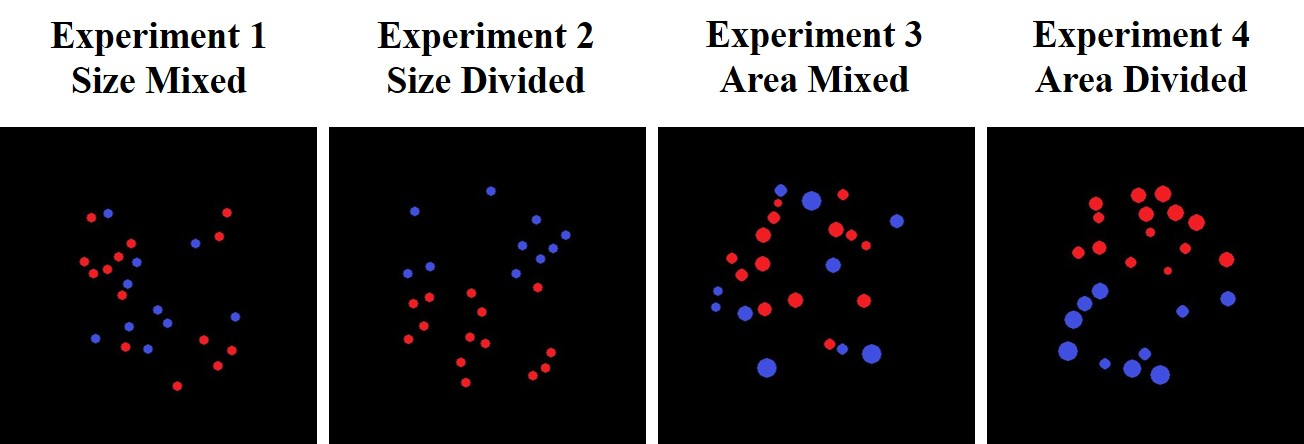
\includegraphics[scale = .45]{Figures/EstSystems/FIG4JPG.jpg}
\caption{Example stimuli from the fixed-item size, mixed color-set design of Experiment 1; the fixed item-size, divided color-set design of Experiment 2; the area-matched mixed color-set design of Experiment 3; and the area-matched divided color-set design of Experiment 4. Each example illustrates a double-target response-condition, where both the red and blue color-sets contain less than 20 items.}
\label{fig:ExpStim}
\end{figure}

\subsection{Participants}
Participants were undergraduate psychology students from the University of Newcastle, Australia, who completed a 90 minute experiment for three course-credits. The number and average age of participants in each of the four experiments are summarized in Table \ref{tab:Ch3_Participants}. All participants reported having normal or corrected to normal vision, and intact color vision.

\begin{table}[htb]
\centering
\caption{Summary table of participant number and mean age across experiments 1--4.}
\label{tab:Ch3_Participants}
\resizebox{\textwidth}{!}{%
\begin{tabular}{lll}
\hline
Experiment                       & Participants (Female) & Age (SD) years \\ \hline
1. Mixed Sets, Fixed Disc Size   & 21 (17)               & 22.67 (4.8)    \\
2. Divided Sets, Fixed Disc Size & 22 (20)               & 22.18 (5.37)   \\
3. Mixed Sets, Fixed Set Area    & 22 (14)               & 23.32 (3.67)   \\
4. Divided Sets, Fixed Set Area  & 21 (16)               & 22.19 (4.37)   \\ \hline \hline
\end{tabular}%
}
\end{table}

\subsection{Stimuli and apparatus}
The apparatus for each experiment was identical, with experiments only varying in stimuli. For simplicity, we will cover the stimuli and apparatus of Experiment 1 in detail, and then only detail the stimuli for each of the remaining experiments.

\subsubsection{Experiment 1}
Testing was conducted in the Newcastle Cognition Laboratory. Stimuli were presented on a 21.5inch Dell S2240L (60Hz) monitor. Stimuli were generated on a Dell Optiplex 7040 computer using python 2.7.14 and the Pygame 1.9.2b package. Responses were made using a standard `qwerty' keyboard. 

Stimuli comprised two sets of non-overlapping red and blue discs. Discs could appear within a central circular field of view, and the position of each disc within this area was sampled randomly (but without spatial overlap). At a viewing distance of 60cm, each disc subtended a visual angle of 0.14 degrees (0.15cm). The circular field of view subtended a visual angle of 9.52 degrees (10cm). Stimuli were presented on a black background. Red and blue colors had RGB values of (241, 29 ,34) and (64, 79, 223) respectively, and were matched for value and chroma using the Munsell color scheme \cite{Cochrane2014}, varying only by hue. Contrast and brightness effects were further controlled using a GLoptic spectis 1.0 photometer.

The first factorial manipulation was the presence or absence of an item-set less-than 20. The 2 (red set: target-present, absent) x 2 (blue set: present, absent) design results in four combinations of target and distractor presentations: double-target, double-distractor, red-target with blue-distractor, and blue-target with red-distractor. The simultaneous presentation of a target and distractor item-set will henceforth be referred to as the conflict-target condition. In addition to these four combinations, we also presented single-target and single-distractor item-sets, (e.g., red-target only, blue-target only, red-distractor only and blue-distractor only). This resulted in eight combinations of item-set presentations, as illustrated in Figure \ref{fig:DFP}. 

The number of red or blue discs presented in each color set varied by condition: target or distractor, high or low salience. The various combinations of response-type and salience-level are illustrated in Figure~\ref{fig:DFP}, with the color-printed integers 10, 14, 29 and 41 representing the set-size for the corresponding color (red or blue). For any one display, the minimum number of discs was 10 and the maximum number of discs (41 + 41) was 82.


\begin{figure}[htb]
\centering 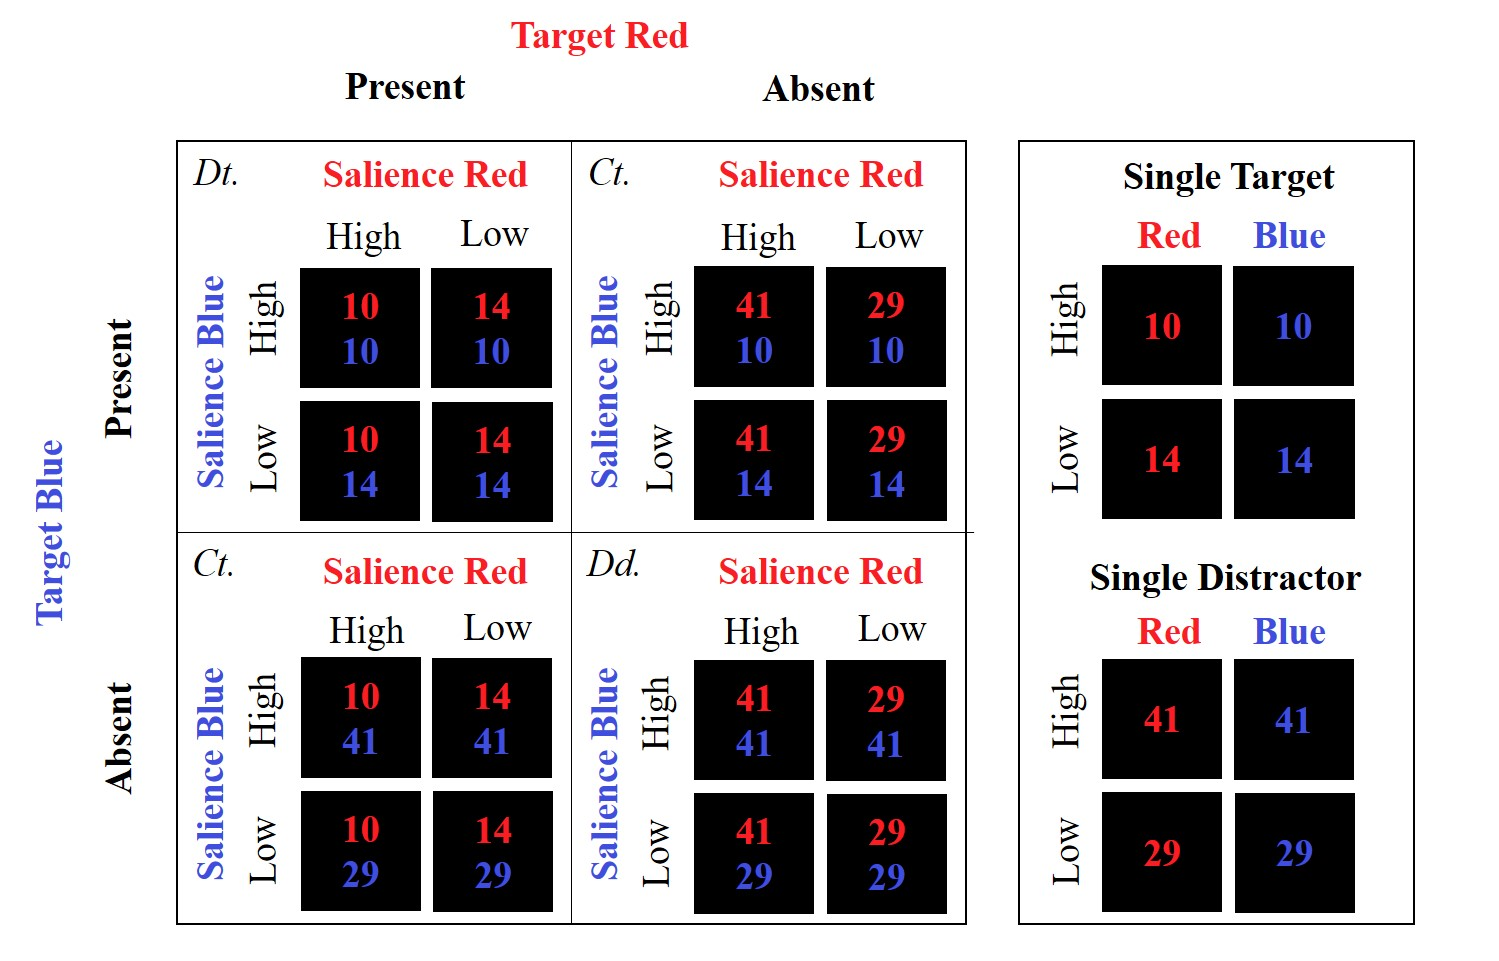
\includegraphics[width = \linewidth]{Figures/EstSystems/FIG5JPG.jpg}
\caption{Expanded double factorial paradigm. Factor one was the presence or absence of a target. Targets were item-sets less than 20. Distractors were item-sets greater than 20. This produced double-target ($Dt$), double-distractor ($Dd$), conflict-target ($Ct$), single-target and single-distractor item-sets. Factor two was the salience manipulation. High-salience item-sets (10 and 41) were further from the criteria (20) than low-salience item-sets (14 and 29). Each black square depicts a stimulus display. In displays where two item-sets were present (left outer-box), four salience combinations were possible: high-high, high-low, low-high and low-low. Single-stimulus displays (right outer-box) were either of high or low salience. Each integer (10, 14, 29 and 41) represent a single item-set presented in their associated color, see figure \ref{fig:ExpStim} for stimulus illustrations.}
\label{fig:DFP}
\end{figure}

\subsubsection{Experiment 2}
Experiment 2 aimed to assess whether the spatial grouping of each color-set aided in the capacity of the estimation-system, or altered the predominant processing-architecture. Stimuli were identical to those of Experiment~1, however each color set was confined to the top or bottom hemisphere of the central circular field-of-view (see second panel of Figure \ref{fig:ExpStim}). The top or bottom position of each color set was randomly selected on each trial. 

\subsubsection{Experiment 3}
Experiment 3 aimed to assess whether low-level covariates of quantity, specifically area, had an impact on the capacity or predominant processing architecture of the estimation system. Similar to Experiment 1, colored item-sets were intermixed within the circular stimulus display. Unlike Experiments 1 and 2, the size (radius) of each item varied. On each trial, the \textit{total} areas of the blue and red color-sets were matched. Color-set area was randomly sampled at the start of each trial and varied within a range of 1540--4620 pixels. This variation in total area was included to reduce the effect of item-size as a predictor of total item-set number. For example, if the total area was always equal to 3000 pixels, on average, the 10 item-set would have relatively large discs and the 41 item-set would always have small discs. Previously, \citeA{HALBERDA_2006} assessed the estimation system in a fixed-size experiment, a fixed item-set area experiment, and a fixed item-set circumference experiment, finding little difference between experimental accuracy or response-times. As such, we did not predict these low-level covariates to change the capacity or processing architecture results.


\subsubsection{Experiment 4}
Experiment 4 was an amalgamation of Experiments 2 and 3. It aimed to assess whether the spatial location of the color-sets and the low-level covariate of area, altered the capacity or predominant processing-architecture of the estimation-system. Experiment 4 controlled for the area of each color-set within a trial, in the same manner as Experiment 3. Similar to Experiment 2, stimuli were presented in either top or bottom hemispheres of the central circular field-of-view (see Figure \ref{fig:ExpStim}).

\subsection{Procedure}
Each participant completed a single 90 minute experimental session. Participants were presented with an information sheet and consent form and answered demographic questions regarding age, gender, handedness, vision and color-blindness. Participants were asked to complete a redundant-target estimation task, in which any display containing a target set (number of discs in set $<$ 20) called for a `yes', target-present response. Any display containing only distractor item-sets, (e.g., double-distractor or a single-distractor only item-set), called for a `no', target-absent response. Participants responded `yes' to the presence of a target with the `z' key and `no' to the absence of a target with the `/' key. Response keys were counter-balanced across participants.

At the start of each trial, participants were directed to look at a central fixation cross, presented for 500ms and followed by a 500ms blank screen. The stimulus display was then presented for 1000ms, followed by a mask for 500ms and a post-mask blank for 2500ms. From the onset of the stimulus, participants had 4000ms to make a response. The trial ended when the participant made a response or the trial timed-out at the conclusion of the response window. 

Participants completed one practice block and 15 experimental blocks, each containing 96 randomly ordered trials. Trial-by-trial accuracy feedback was provided during the practice block. Each block contained 12 double-target trials, 12 double-distractor trials, 24 conflict-target trials, 24 single-target trials and 24 single-distractor trials, presented in a random order. These trials were evenly distributed among the constituent salience levels. For example, three trials were presented from each double-target salience combination --- 12 in total. By comparison, six trials were presented from each of the red and the blue, single-target high and single-target low salience conditions --- 24 in total. Not including practice trials, each subject completed 180 double-target trials, 180 double-distractor trials, 360 conflict-target trials (180 target-red, 180 target-blue), 360 single-target trials (180 target-red, 180 target-blue) and 360 single-distractor trials (180 distractor-red, 180 distractor-blue). In total, subjects completed 1440 experimental trials with a 5:3 yes/no response bias. The probability of a target item-set in one color, (e.g., red), given a target item-set in the other color, (e.g., blue), was 0.33 \cite{mordkoff1991}.

\section{Data analysis}
Incorrect trials, and trials with response times less than 150 ms or greater than the 97.5$^{th}$ percentile were excluded from analysis. Participants' data were included if their total accuracy was $>80\%$ correct, \emph{and} their conditional accuracy in each of the six target conditions was $>66\%$. All repeated-measures ANOVAs were corrected for violations of sphericity, where appropriate, using the Greenhouse-Geisser correction. Post-hoc paired $t$-tests were corrected for family wise error using the Bonferroni method. 

Workload capacity was assessed through the redundant target effect \cite<RTE; >{miller1982divided, eidels2008similarity}, the capacity coefficient and resilience difference function. The RTE assesses the cost or gain associated with processing an additional, redundant target item-set, when compared to the processing of a single target item-set in isolation. A negative RTE indicates a cost to workload capacity. The RTE can be expressed as RTE = $min$(\mRT{RedTarget}, \mRT{BlueTarget}) - \mRT{DoubleTarget}, such that a negative RTE indicates a redundancy cost. The RTE was tested for significance at the cumulative distribution level through a series of non-parametric Kolmogrov-Smirnov (KS) tests, investigating the distribution ordering to determine whether $min$[$F_{RedTarget}$($t$), $F_{BlueTarget}$($t$)] $>$ $F_{DoubleTarget}$($t$). As the KS test is a conservative measure, we followed the method reported by \citeauthor{johnson2010systems} \citeyear{johnson2010systems} and adopted a more liberal alpha ($p$ $<$ 0.15) to determine significance.

Processing architecture was assessed for double-target conditions (where red and blue item-sets both satisfied the criterion and each contained less than 20 items) using the mean interaction contrast (MIC) and its distributional counterpart, the survivor interaction contrast [SIC($t$)]. The MIC distinguishes between parallel self-terminating (MIC $>$ 0), parallel exhaustive (MIC $<$ 0), and serial models (MIC = 0). Due to the construction of the MIC, a significance test of the interaction term between high and low salience levels can establish whether the model is parallel. The SIC($t$) can distinguish between the two parallel models, and additionally the serial self-terminating and serial exhaustive models, however requires selective influence to hold for each manipulation of salience at the level of the cumulative distribution. We tested a criterion for the presence of selective influence within double-target conditions for each subject individually using the following non-parametric KS tests \cite<alpha $p$ $<$ 0.15; see>{johnson2010systems}:

\noindent
\begin{align*}
S_{\rm LL}(t) &< \left\{S_{\rm LH},S_{\rm HL}\right\} \textrm{ is significant}\\
S_{\rm LL}(t) &> \left\{S_{\rm LH},S_{\rm HL}\right\} \textrm{ is not significant}\\
S_{\rm HH}(t) &> \left\{S_{\rm LH},S_{\rm HL}\right\} \textrm{ is significant}\\
S_{\rm HH}(t) &< \left\{S_{\rm LH},S_{\rm HL}\right\} \textrm{ is not significant}\\
S_{\rm HH}(t) &< S_{\rm LL}(\t)  \textrm{ is significant}
\end{align*}

Until fairly recently, inference on the SIC($t$) was limited to visual inspection. \citeauthor{houpt2010statSIC} \citeyear{houpt2010statSIC} developed null-hypothesis significance tests (NHST) to more formally diagnose deviations from a zero SIC. However, these tests are limited by the standard pitfalls of NHST. In particular, the `null' signature actually corresponds to the serial OR model, making direct inference about that model difficult under the NHST framework. More recently, \citeA{houpt2017bayesSIC} developed a non-parametric Bayesian approach for categorizing SIC($t$). The approach is based on a Dirichlet process that samples thousands of SIC functions based on the empirical probabilities of each condition at certain quantiles, and categorizes each sample based on which model shape it best approximates (as illustrated back in Figure \ref{fig:SIC}).

The Bayesian framework has the advantage of quantifying the strength of evidence for each model (allowing comparison of model weights), and also allows direct inference about the serial models. We implemented this Bayesian approach to help categorize our SIC models. We used a uniform prior on the model space such that the prior likelihood of sample corresponding to a given SIC state (neither, one, or both of a positive or negative deviation at some time \textit{t}) was equally likely. This uniform prior has the advantage of giving very weak evidence for all models in the case an SIC is truly uninformative, whereas the approach presented by \citeauthor{houpt2017bayesSIC} tended to show strong evidence of serial processing in such cases \cite{houpt2017bayesSIC}. To be sure, testing confirmed that using the uniform prior distribution did not hurt model recovery when applied to the simulated data from \citeauthor{houpt2017bayesSIC}'s (2017).

In addition to the SIC analyses, we implemented the hierarchical MIC estimation procedure introduced by \cite{houpt2017hierarchical}.
This analysis involved hierarchically estimating parameters of a gamma distribution for each subject's conditional response-time distribution, where the rate parameter of each distribution was constrained by a higher-order 'MIC state' model. This procedure allows a parametric evaluation of evidence for processing architecture at the MIC level --- serial (MIC = 0), parallel minimum-time (MIC $>$ 0) and parallel maximum-time (MIC $<$ 0). Using these two Bayesian approaches we were able to obtain converging Bayesian evidence for serial and parallel processing architectures using both non-parametric (Bayesian SIC), and parametric (Bayesian MIC) approaches. 

\section{Results}
In these results, we will focus on system capacity, conflict-target resilience (\ie architecture and workload), and target processing architecture. For clarity of exposition, experiments are presented together for each of the above sections.

\subsection{Group Means}
Participants with conditional accuracy $< 66\%$ or total accuracy $< 80\%$ were excluded from analysis. Three participants were excluded from Experiment 1 and Experiment 3, and two participants were excluded from Experiment 2 and Experiment 4 due to low accuracy. Accuracy was high for all remaining subjects in Experiment 1 (\Acc{0.94}{0.04}), Experiment 2 (\Acc{0.94}{0.03}), Experiment 3 (\Acc{0.93}{0.03}) and Experiment 4 (\Acc{0.93}{0.04}). Error rates were too low to afford statistically meaningful comparisons between response conditions. As such, the remaining results focus exclusively on our primary metric, response-time.

The following response-time results section focuses on red single-target (Rt), blue single-target (Bt) and double-target (Dt) responses, as these conditions form the basis of the subsequent workload capacity analysis. These response-sets are formed from the combination of their nested salience levels. Red single-target responses are formed from the high (H) and low (L) red target-salience levels, and double-target responses include combinations of HH, HL, LH and LL red-and-blue target-salience levels.

\subsubsection{Experiment 1: Fixed Sized Items, Mixed Color-Sets}
Mean response-time (mRT) results for Experiment 1 are plotted as black markers towards the left of Figure \ref{fig:MeanRTAcc}. Within the target conditions, there was a significant effect of workload (number of targets) on response-time (\Fval{1.47}{25}{27.34}{$<$ .001}, \etap{0.62}). Post-hoc paired sample $t$-tests showed red-target responses (\rt{551}{56}) were faster than double-target responses (\rt{589}{68}); \tval{17}{5.122}{$<$ .001}, $d$ = 1.21). Likewise, blue-target responses (\rt{546}{53}) were faster than double-target responses (\tval{17}{6.063}{$<$ .001}, $d$ = 1.43). Red-target and blue-target responses did not significantly differ (\tval{17}{1.325}{= 0.20}, $d$ = 0.31). Bonferroni corrections were used for multiple comparisons, where appropriate. 

\begin{figure}[htb]
\centering 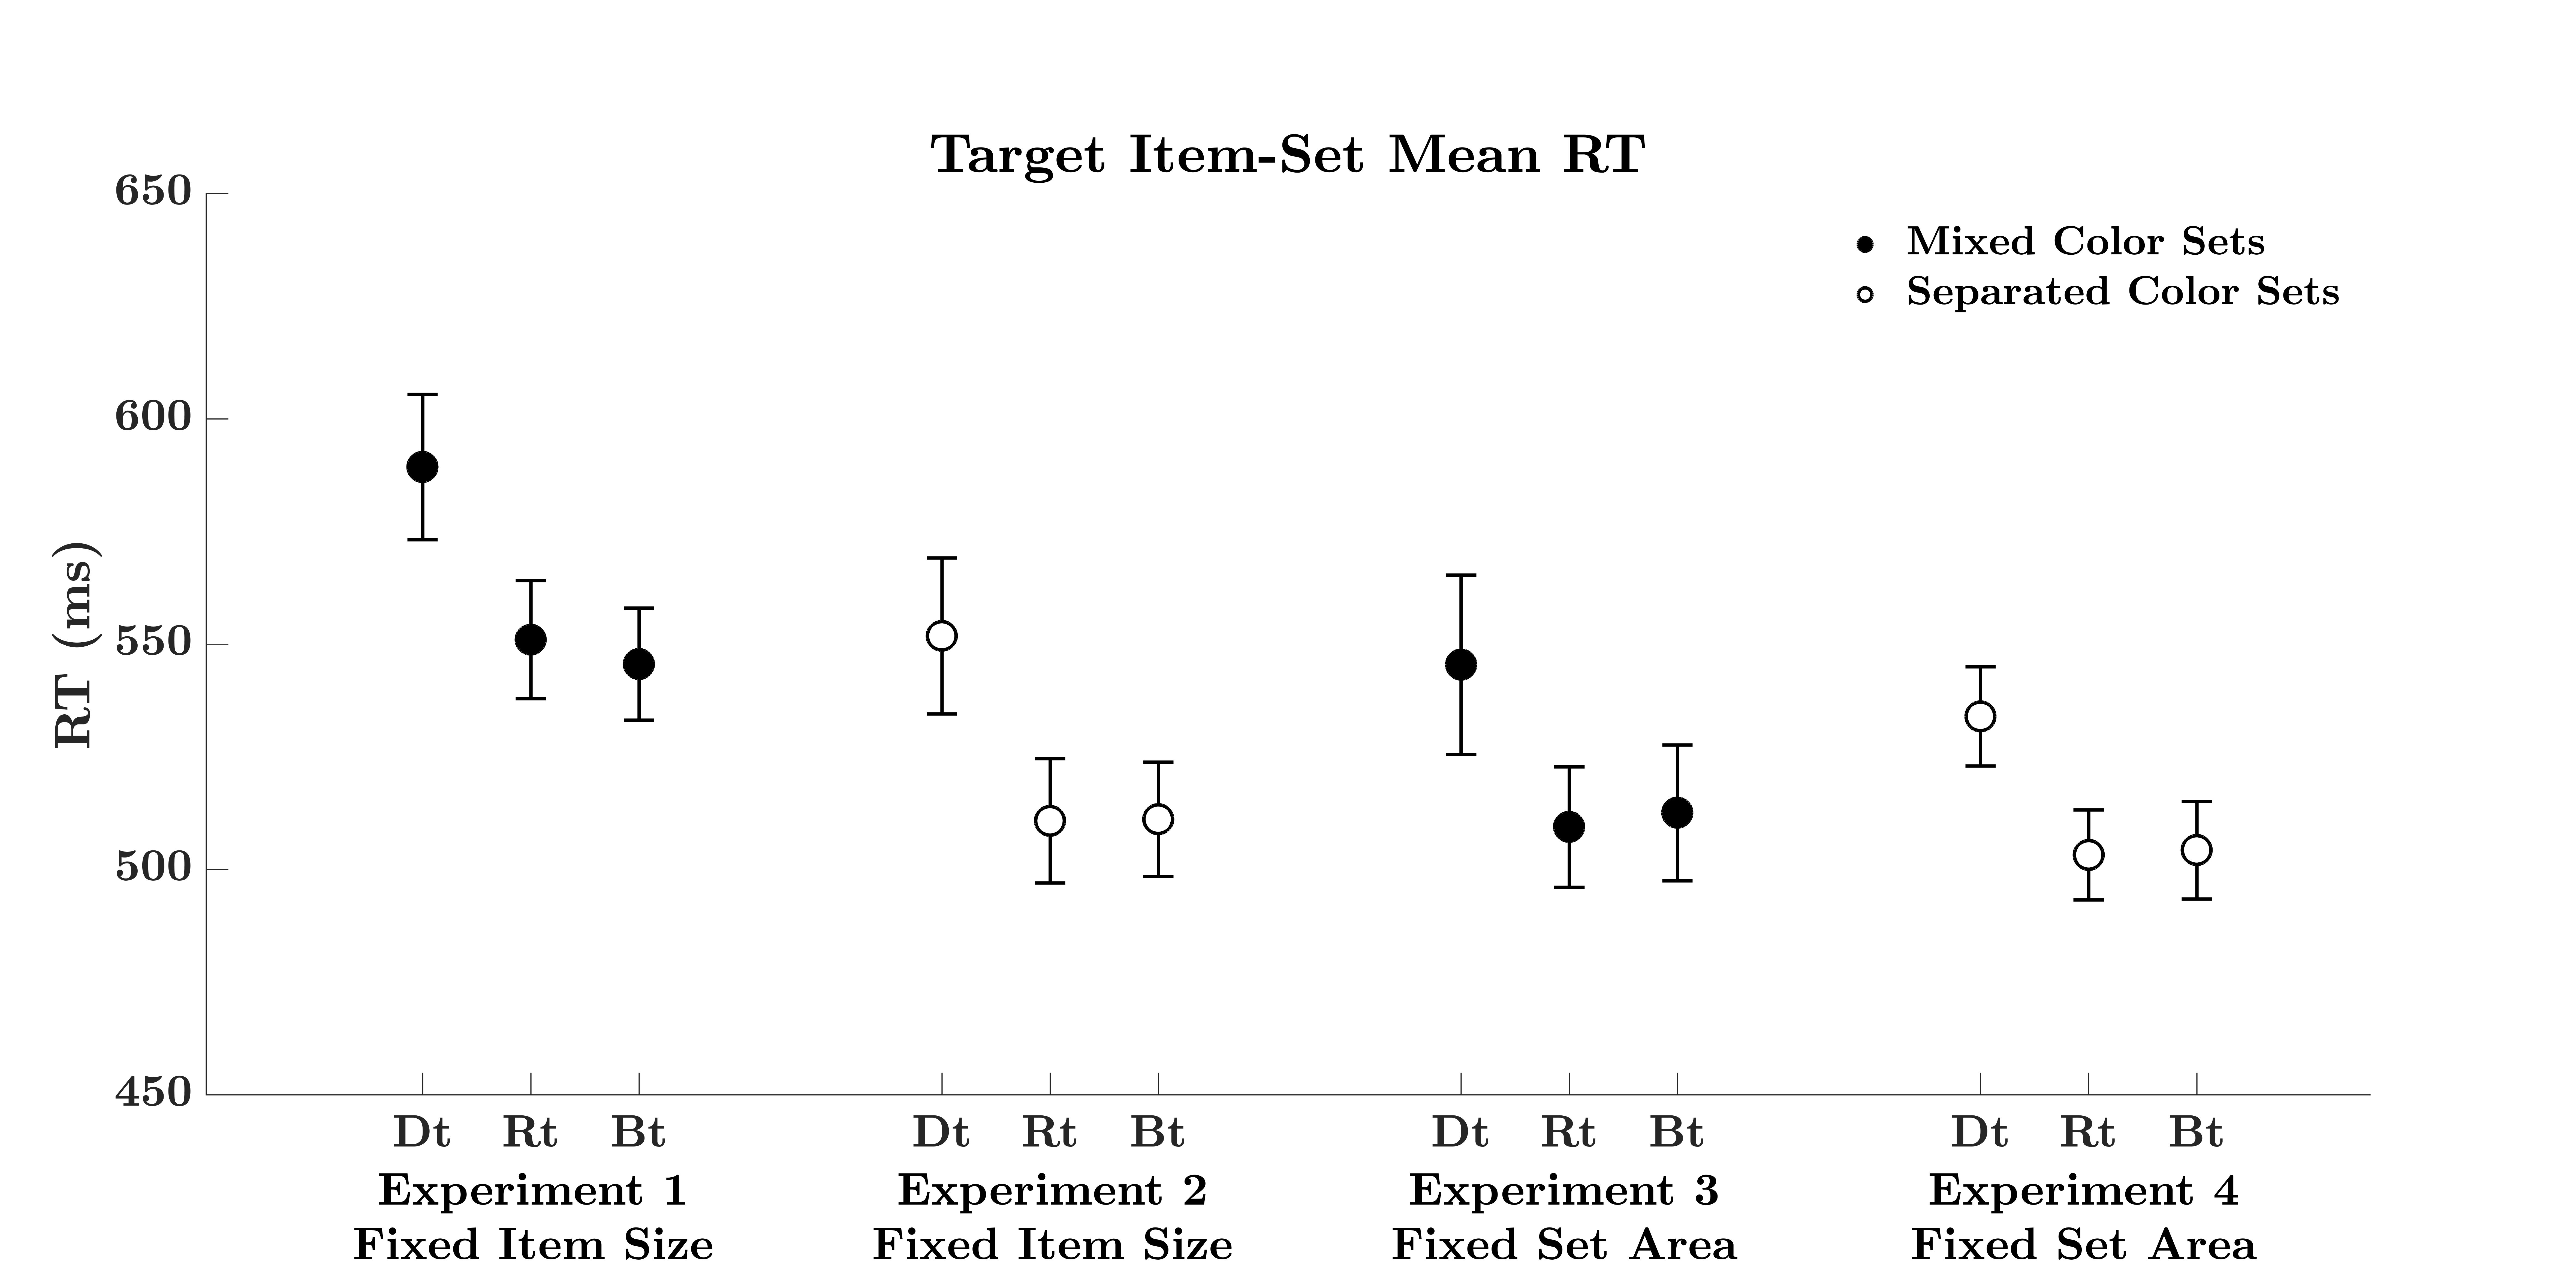
\includegraphics[width=\linewidth]{Figures/EstSystems/FIG6JPG.jpeg}
\caption{Mean response-time plots for double-target (Dt), red single-target (Rt) and blue single-target (Bt) response sets, across Experiments 1 ($N$ = 18), 2 ($N$ = 20), 3 ($N$ = 19) and 4 ($N$ = 19). Plots illustrate the slowing of double-target responses within each experiment, relative to their single-target counterparts. Error bars represent $\pm$ one standard error of the mean.}
\label{fig:MeanRTAcc}
\end{figure}

\subsubsection{Experiment 2: Size Divided Color-Sets}
Mean response times for Experiment 2 are plotted as white markers towards the left of Figure \ref{fig:MeanRTAcc}. There was a significant effect of target-type on RT (\Fval{1.22}{23.25}{36.08}{$<$ .001}, \etap{0.66}). Red-target responses (\rt{511}{62}) were faster than double-target responses (\rt{551}{77}; \tval{19}{6.84}{$<$ .001}, $d$ = 1.53), and blue-target responses (\rt{511}{57}) were faster than double-target responses (\tval{19}{5.807}{$<$ .001}, $d$ = 1.3). Red and blue single-target responses were not significantly different (\tval{19}{-0.136}{= 0.89}, $d$ = -0.03).

\subsubsection{Experiment 3: Area Mixed Color-Sets}
Mean response times for Experiment 3 are plotted as black markers towards the right of Figure \ref{fig:MeanRTAcc}. There was a significant effect of target-type on response-time (\Fval{1.44}{25.89}{12.82}{$<$ .001}, \etap{0.42}). Post-hoc paired $t$-tests revealed red-target responses (\rt{509}{58}) were faster than double-target responses (\rt{545}{87}); \tval{18}{4.184}{$<$ .01}, $d$ = 0.96), and blue-target responses (\rt{513}{66}) were faster than double-target responses (\tval{18}{3.504}{$<$ .01}, $d$ = 0.8). Red-target and blue-target responses were not significantly different (\tval{18}{-0.638}{= 0.53}, $d$ = -0.15).

\subsubsection{Experiment 4: Area Divided Color-Sets}
Mean response times for Experiment 4 are plotted as white markers towards the right of Figure \ref{fig:MeanRTAcc}. In line with previous experiments, there was a significant effect of target-type on response-time (\Fval{1.46}{26.28}{30.39}{$<$ .001}, \etap{0.63}). Post-hoc paired $t$-tests showed red-target responses (\rt{503m}{44}) were faster than double-target responses (\rt{534}{48}); \tval{18}{6.414}{$<$ .001}, $d$ = 1.47), and blue-target responses (\rt{504}{48}) were faster than double-target responses (\tval{18}{5.529}{$<$ .001}, $d$ = 1.27). Red-target and blue-target responses were not significantly different (\tval{18}{-0.362}{= 0.72}, $d$ = -0.08).

\subsection{Redundant Target Effects}
As reported in Group Means section, double-target responses were significantly slower than single-target responses. This $redundancy$ $cost$, displayed as a negative RTE, was observed in all experiments and suggests that the addition of a second target slows the estimation-system, a hallmark of limited capacity processing. However, a redundancy cost at the group level does not dictate a redundancy cost for each subject. The following section examines the direction and significance of the redundant target effect for each subject.

\subsubsection{Experiment 1: Size Mixed Color-Sets}
Individual redundant target effects and corresponding significance values are plotted in the top-left panel of Figure \ref{fig:GroupRTE}. Seventeen subjects in Experiment 1 recorded a significant redundancy cost at the distributional level (KS $<$ .15), suggesting these individuals experienced capacity limitations when processing two target item-sets. One subject exhibited a redundancy cost, however, did not reach significance at the level of the distribution.

\begin{figure}[hbt]
\centering 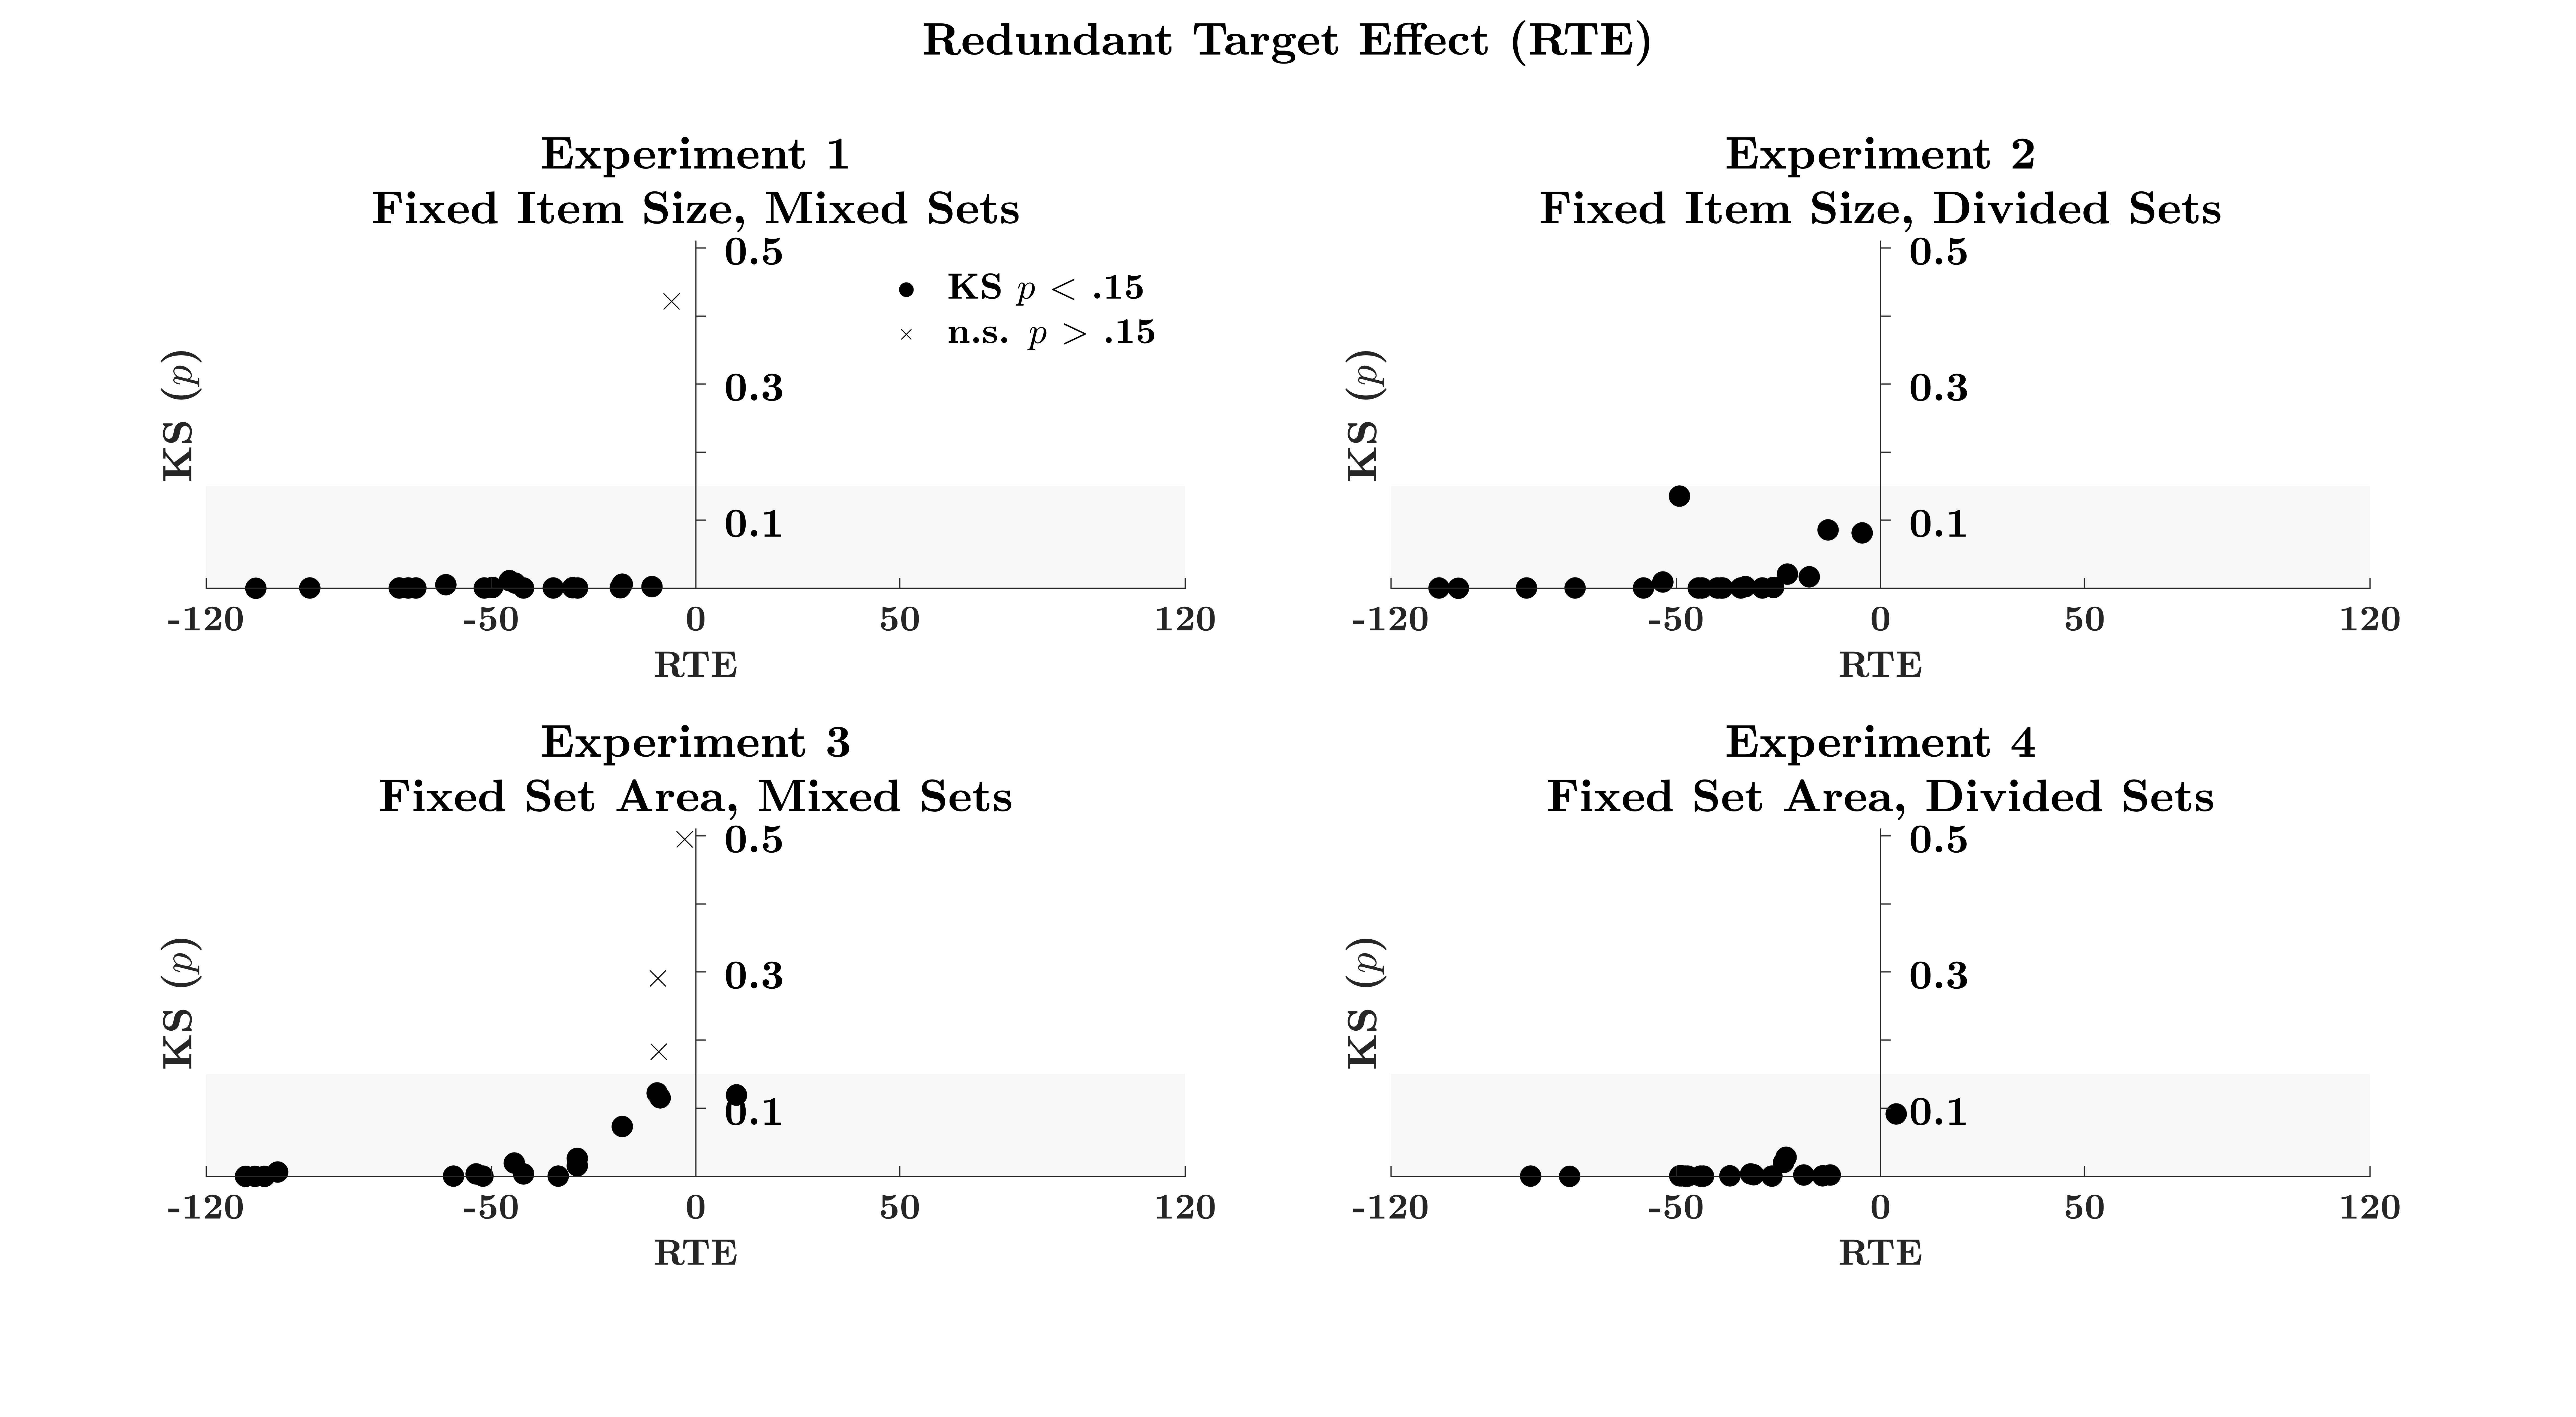
\includegraphics[width=\linewidth]{Figures/EstSystems/FIG7JPG.jpeg}
\caption{Significance values for individual subject's redundant target effects (RTE) plotted separately for Experiments 1 ($N$ = 18), 2 ($N$ = 20), 3 ($N$ = 19) and 4 ($N$ = 19). Negative RTE values denote a redundancy cost. Each subject is plotted as an individual marker, black markers indicate a significant RTE (KS $p < .15$), and X markers indicate a non-significant RTE (KS $p > .15$). Across the four experiments, most subjects exhibited a significant redundancy cost. \newline \emph{\bf Note:} One outlier was excluded from the Experiment 4 RTE plot, RTE = -10 and $p = 0.63.$}
\label{fig:GroupRTE}
\end{figure}


\subsubsection{Experiment 2: Size Divided Color-Sets}
Individual subject's redundant target effects and corresponding significance values are plotted in the top-right panel of Figure \ref{fig:GroupRTE}. All 20 subjects exhibited significant redundancy costs at the level of the distribution (KS $<$ 0.15). 

\subsubsection{Experiment 3: Area Mixed Color-Sets}
Individual subject's redundant target effects and corresponding significance values are plotted in the bottom-left panel of Figure \ref{fig:GroupRTE}. Fifteen subjects exhibited a significant redundancy cost at the level of the distribution. One participant recorded a redundancy $gain$ (positive RTE) at the level of the distribution, in contrast to the trend of most subjects in this experiment. Three subjects recorded a redundancy cost, but did not reach significance at the distribution level.

\subsubsection{Experiment 4: Area Divided Color-Sets}
Individual subject's redundant target effects and corresponding significance values are plotted in the bottom-right panel of Figure \ref{fig:GroupRTE}. Eighteen subjects recorded a significant redundancy cost at the level of the distribution. One subject recorded a redundancy cost but did not reach significance at the level of the distribution. This subjects was removed as an outlier from the Experiment 4 RTE plot and recorded an RTE = -10 ($p = 0.63$). 

\subsection{Capacity Coefficient}
Nearly all participants, in all four experiments, showed a significant redundancy cost (negative RTE) at the level of the distribution when estimating two target item-sets. The ubiquity of this finding suggests that the estimation of multiple item-sets is a limited capacity process, experienced by all individuals regardless of the perceptual covariate of item-set area, or whether item-sets were spatially overlapping or separate. For interpretation of individual subject's workload capacity across the entire response-time range, we may also consider the capacity coefficient. The capacity coefficient allows clear interpretation of performance limitations, as it assays performance against an established benchmark (unlimited capacity, independent-channels parallel model). 

Group mean and individual capacity coefficient (C($t$)) values for Experiments 1--4 are plotted in Figure \ref{fig:GroupCapacity}. Focusing on the group mean \Ct results from Experiment 1 (top-left panel), \Ct $<$ 1 for all of the response-time range, suggesting a limited workload capacity processing system. Furthermore, \Ct hovers below the Grice lower-bound for all of the response-time range. This suggests a system with severe capacity limitations. In line with the group results, all individual \Ct values (illustrated by gray markers) also hover at \Ct $<$ 1 and suggest limited workload capacity. Individual low-bounds present at approximately \Ct = 0.5, with all individual \Ct scores resting at or below the low-bound for the majority of the response-time range (individual \Ct plots for each experiment can be found in the supplementary materials, Figures \ref{fig:Indiv_Cap_Ex1}--\ref{fig:Indiv_Cap_Ex4}). In line with the group results, this suggests most individuals experienced severe capacity limitations when estimating multiple item-sets. Results from Experiments 2--4 show similar trends and support severely limited workload capacity processing systems in all subjects.

\begin{figure}[tbh]
\centering 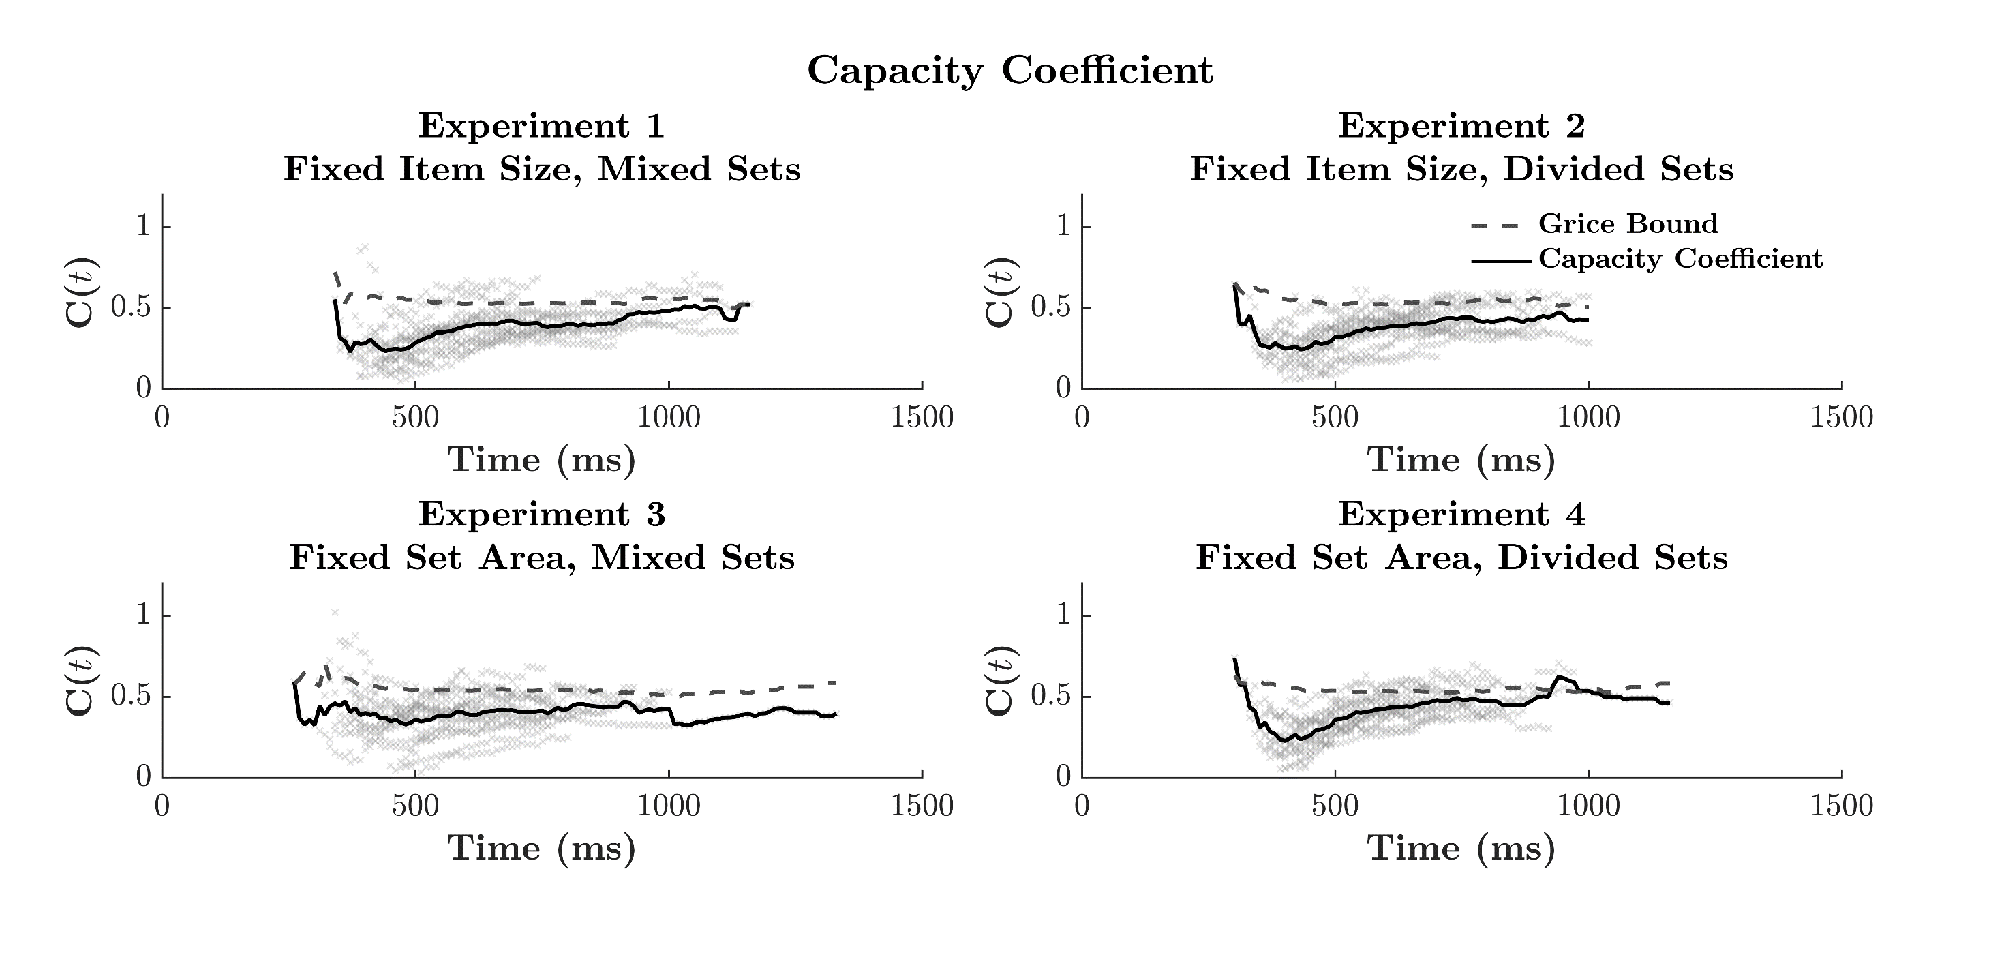
\includegraphics[width=\linewidth]{Figures/EstSystems/FIG8JPG.pdf}
\caption{Capacity coefficient (C($t$)) plots for target-present responses in Experiments 1--4. Group mean \Ct is plotted in black with the Grice lower-bound, an estimate of severe capacity limitations, depicted by the dashed line. Individual participant \Ct values are illustrated by gray markers and mostly fall at or below the group Grice bound, indicating severe capacity limitations across all experiments.}
\label{fig:GroupCapacity}
\end{figure}

Analysis of the capacity coefficient extends previous RTE analysis, showing that all subjects estimated multiple target-sets with limited workload capacity. Furthermore, performance of most subjects was at or below the Grice-bound, suggesting they may have experienced capacity limitations typically associated with serial processing architectures. We now consider the unique assessments of processing architecture and workload, provided by the resilience difference function, and compare these to our capacity coefficient results. 

\subsection{Resilience Function Analysis} 
Resilience difference (R$_{diff}$($t$)) values for the group mean as well as individual subjects, for low target-salience trials on each of the four experiments, are plotted in Figure \ref{fig:RdiffLow}. Interpretation of these results can be aided by comparison to \Rd predictions, presented in Figure \ref{fig:Rd}. Focusing on Experiment 1 group mean, \Rd hovers around zero, for most of the response-time range. This aligns with the prediction of a parallel minimum-time unlimited-capacity processing system. 
In line with the group results, most individual \Rd values (illustrated by gray markers) hover around \Rd = 0. Results from Experiments 2--4 show similar trends, in line with the predictions of a parallel minimum-time unlimited-capacity model. We replicated the \Rd analysis for high target-salience, and the results were again similar, in line with a parallel minimum-time unlimited-capacity processing system (see Figure \ref{fig:RdiffHigh} in the supplementary materials). Overall then, there seem to be some discrepancy between the capacity coefficient results, which support severely limited workload-capacity (potentially associated with serial architectures), and the resilience difference results, which support unlimited capacity that is often associated with parallel architectures. The fidelity of these claims can be directly assess through our next system measures, the MIC and SIC. 

\begin{figure}[tbh]
\centering 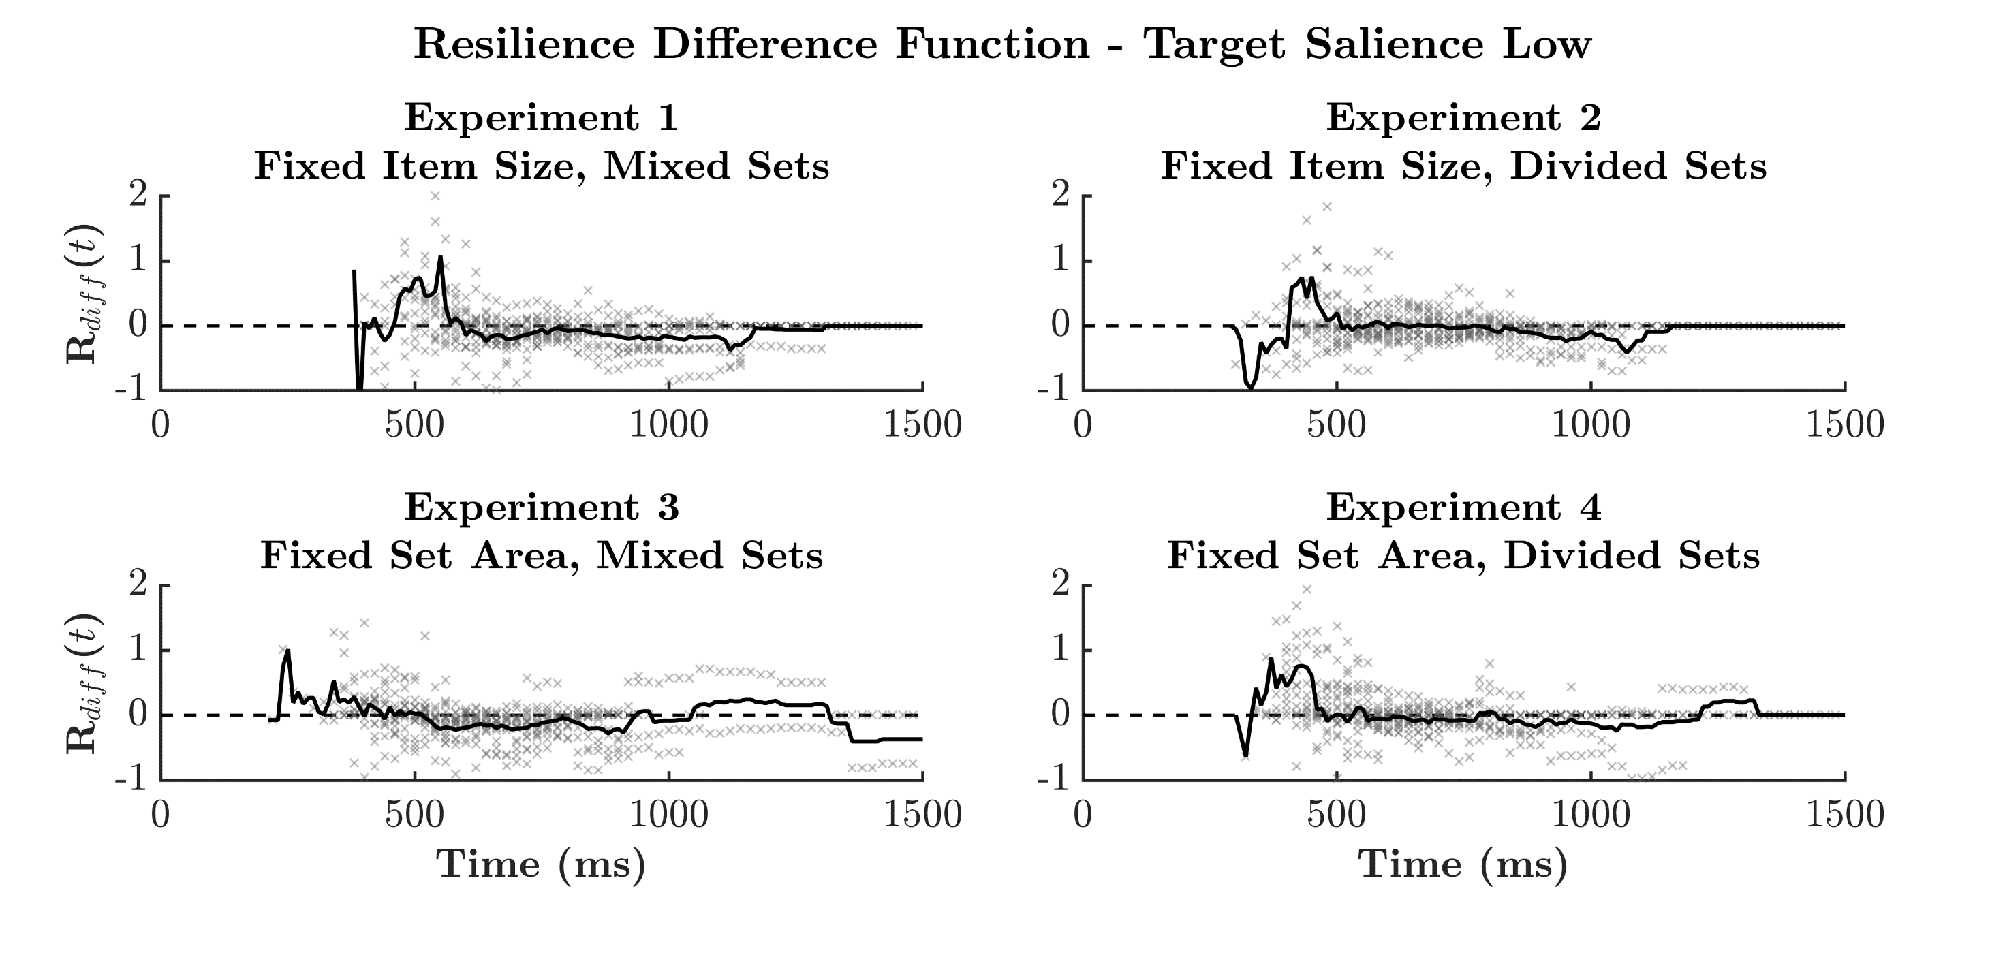
\includegraphics[width=\linewidth]{Figures/EstSystems/FIG9JPG.pdf}
\caption{Resilience difference plots for Experiments 1 – 4 when target salience is low. Black lines depict the average resilience difference function across subjects, while grey markers illustrate individual subject’s resilience difference functions. Average plots show a trend towards \Rd = 0, supporting predictions made by an unlimited-capacity parallel minimum-time processing system.}
\label{fig:RdiffLow}
\end{figure}

\subsection{Double-Target Processing Architecture}
In the following section, we report the MIC and SIC calculated from the response-time differences between salience manipulations --- high-high (HH), high-low (HL), low-high (LH) and low-low (LL) --- nested within the double-target response type. For valid interpretation, the mean interaction contrast (MIC) requires a successful manipulation of salience within both color-sets. This was assessed through a between-subject ANOVA conducted separately for each subject. For the MIC, a statistical interaction between the salience levels of each color-set acts as a test for parallel processing architectures and is therefore reported. Interpretation of the survivor interaction contrast (SIC) requires selective influence to hold at the level of the survivor functions (see the Data Analysis section for details). These tests were completed for each subject, and only subjects who met the criteria for selective influence are reported in Table \ref{table:Exp1_DT}. Finally, we report the Bayes factor for the winning MIC model, as MIC group posterior and the associated best MIC model fit. To foreshadow the outcomes, only a limited number of subjects satisfied the included criteria and could be categorized by processing architecture. For clarity of exposition, we first summarize the results of classified subjects across all experiments, then present a breakdown by individual subjects. 

MIC values for subjects who met SIC and MIC inclusion criteria in Experiments 1--4 are illustrated in the left panel of Figure \ref{fig:MICandProp_AB}. The majority of subjects in each experiment recorded a positive MIC value, supporting parallel minimum-time processing architectures. The right panel of Figure \ref{fig:MICandProp_AB} shows the proportion of each architecture, using the Bayesian SIC and hierarchical Bayesian MIC methods. Each bar represents the total number of (classified) subjects in a given experiment, and the shaded regions mark the relative proportion of subjects based on the way they enumerated two target sets (in parallel, serial). As expected, parallel processing architectures were applied by a majority of subjects in all experiments. Minimum-time stopping-rules were most common in Experiments 1--3, while in Experiment 4 most subjects used a maximum-time stopping rule. Individual results are  presented next. 

\begin{figure}[hbt]
\centering 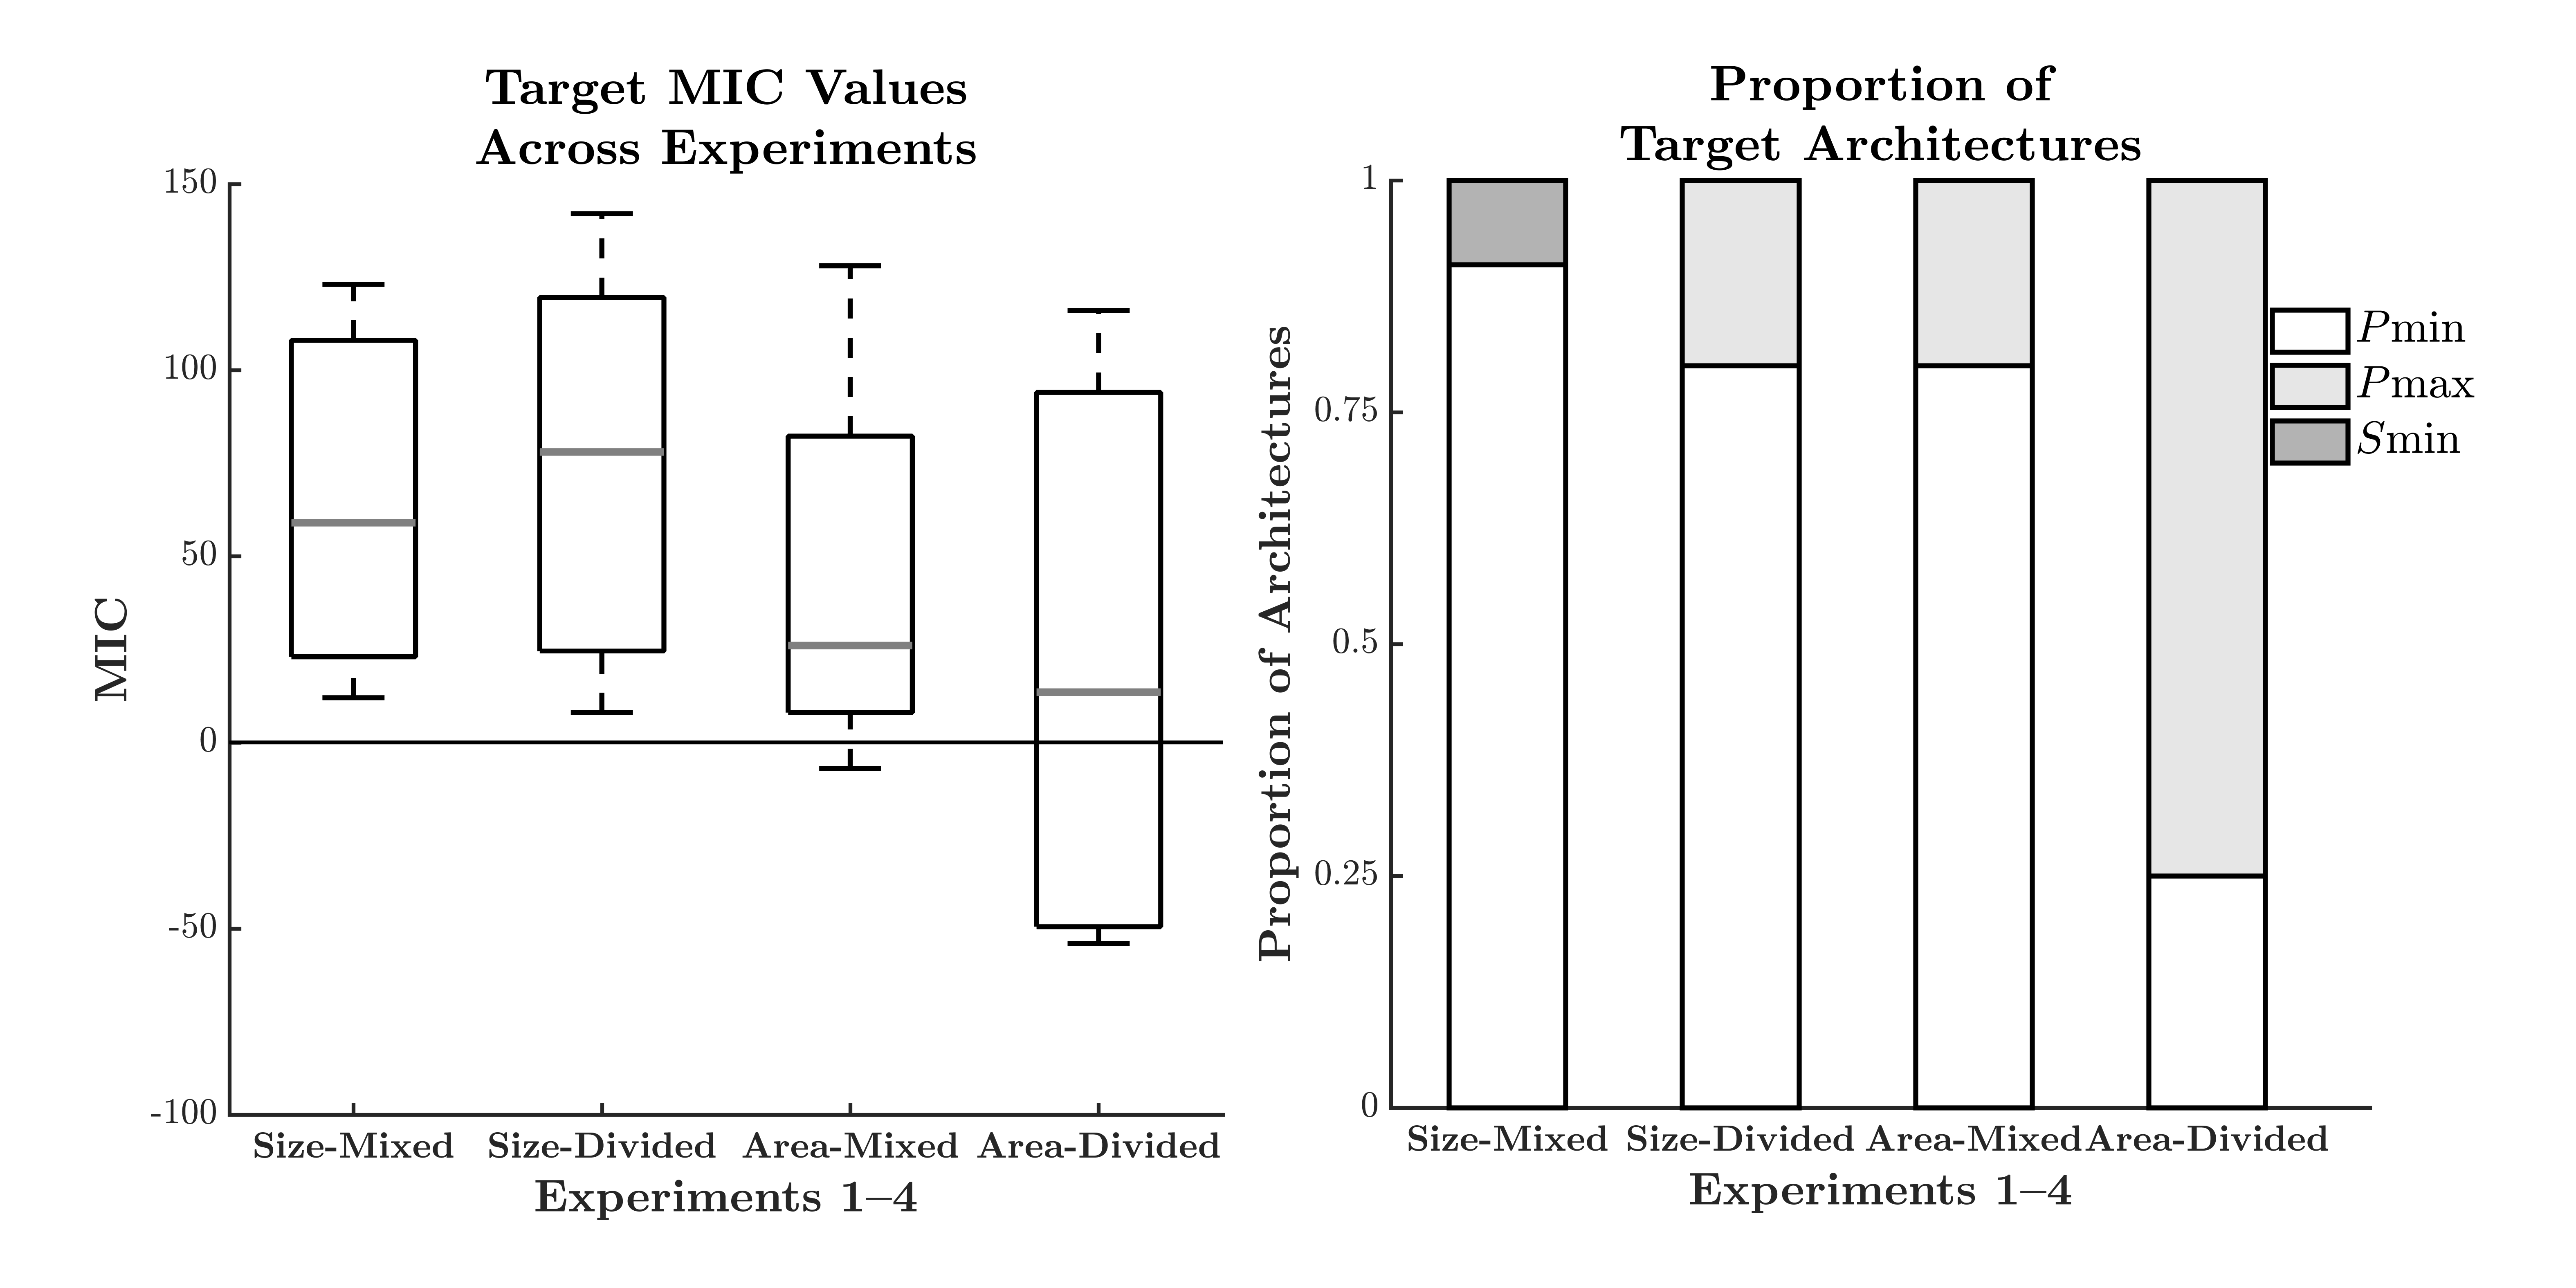
\includegraphics[width=\linewidth]{Figures/EstSystems/FIG10JPG.jpg}
\caption{MIC values (left) and the proportion of categorized processing architectures (right) for subjects in Experiments 1--4. Proportions are relative to the total number of subjects who could be classified using MIC and SIC significance testing. Ten subjects were categorized in Experiment 1, five subjects in Experiment 2, five subjects in Experiment 3 and four subjects in Experiment 4. \\ \textbf{Note.} $P$min = parallel minimum-time, $P$max = parallel maximum-time, $S$min = serial minimum-time.}
\label{fig:MICandProp_AB}
\end{figure}

\subsubsection{Experiment 1: Fixed Size, Mixed Color-Sets}
Individual MIC and SIC results are reported in Table 1, along with each subjects categorized candidate architecture. Subject categorization started with assessment of target salience effects. For each subject we tested for a main effect of red-target salience (R) and blue-target salience (B). Due to the construction of the MIC, a significant interaction of red-target and blue-target salience provides supportive evidence of a parallel processing architecture, while MIC valence indicates the stopping-rule. 


Stopping-rule refers to whether only one item-set (minimum-time rule) or both item-sets (maximum-time rule) need to be enumerated before a correct response may be given. This is different than the localized search-strategy employed when enumerating items \textit{within} each set. All reported subjects met the criteria for selective influence at the level of the distributions, assessed through a series of non-parametric KS test (see Data Analysis).

Subjects were categorized based on their SIC functions, classified using the newly developed non-parametric Bayesian SIC assessment techniques provided by \citeA{houpt2017bayesSIC}, supplemented by visual inspection of the MIC and ANOVA results\footnote{MIC interpretation was aided by consideration of MIC processing architecture plots. Visual assessment of the MIC plot has been beneficial in previous studies when categorizing processing architectures, however, is less robust than our recent method of classification, which utilizes the SIC.}. The new Bayesian SIC assessment techniques of \citeA{houpt2017bayesSIC} categorizes the subject SIC by processing architecture and stopping-rule, and further provides a model probability for observing a given processing architecture, (e.g., parallel minimum-time), relative to the four alternative architectures, (i.e., parallel maximum-time, coactive, serial minimum-time and serial maximum-time). As such, our criteria for a conclusive model architecture was determined via Bayesian SIC categorization where the candidate model displayed a selection probability greater than $0.5$, (i.e., where the candidate model was deemed more probable than all alternative model accounts). Finally, our results were augmented by a hierarchical Bayesian MIC analysis \cite{houpt2017hierarchical}, which takes into account data across all valid subjects in each experiment. For simplicity, we report the Bayes factor (BF$_{10}$) in favor of the best fitting model, identified in the far right columns of Table \ref{table:Exp1_DT}. 

\begin{table}[htb]
\caption{Individual double-target MIC and SIC results from Experiment 1. From left to right, ANOVA main effects for red target salience (R) and blue target salience (B), MIC value and interaction significance,  Bayesian SIC model probabilities and associated architectures, and Bayes factor values from the hierarchical MIC analysis with associated processing architectures. Note, P - Parallel, S - Serial.}
\centering 
\begin{tabular*}{\textwidth}{l @{\extracolsep{\fill}} lllllll}
\hhline{-------}
\textbf{Sub  } & \textbf{\begin{tabular}[c]{@{}c@{}}Main \\ Effects\end{tabular}} & \textbf{MIC} & \textbf{SIC} $\mathbb{P}$ & \textbf{SIC Model} & \textbf{BF$_{10}$} & \textbf{MIC Model} \\  
\hhline{-------}
101 & R \& B & 53*    & \textbf{0.73} & \textbf{P Min-Time} & \textbf{10.69}  & \textbf{P Min-Time} \\ 
102 & R \& B & 33     & \textbf{0.64} & \textbf{P Min-Time} & \textbf{7.04}  & \textbf{P Min-Time} \\ 
103 & R \& B & 117*** & \textbf{0.83} & \textbf{P Min-Time} & \textbf{24.02} & \textbf{P Min-Time} \\       
104 & R \& B & 23 	  & 0.35 		  &         P Min-Time  & \textbf{6.38}  & \textbf{P Min-Time} \\    
107 & R \& B & 108**  &\textbf{0.91}  & \textbf{P Min-Time} & \textbf{24.83}  & \textbf{P Min-Time} \\  
110 & R \& B & 77* 	  &\textbf{0.78}  & \textbf{P Min-Time} & \textbf{13.11} & \textbf{P Min-Time} \\        
111 & R \& B & 21	  &0.46           &         P Min-Time  & \textbf{4.13}   & \textbf{P Min-Time} \\ 
114 & R \& B & 123*** &\textbf{0.85}  & \textbf{P Min-Time} & \textbf{25.79} & \textbf{P Min-Time} \\      
116 & R \& B & 12  	  &0.42           &         P Min-Time  & \textbf{5.35}  & \textbf{P Min-Time} \\         
117 & R \& B & 65* 	  &0.33           &         S Min-Time  & \textbf{9.83}  & \textbf{P Min-Time} \\    
\hhline{~~~~---}
~&~&~&~& \textit{MIC Group Posterior} & \textbf{6.89} & \textbf{P Min-Time} \\
\hhline{-------} \hhline{-------}
\multicolumn{7}{p{\textwidth}}{ MIC interaction significance tests were conducted at \textit{p} $<$ .33*, \textit{p} $<$ .05** and \textit{p} $<$ .01***. Conclusive model architectures were based upon an SIC model selection probability $>$ 0.5 and are displayed in bold font. MIC models with at least moderate evidence (BF$_{10}$ $>$ 3) are also displayed in bold font.}
\end{tabular*} 
\label{table:Exp1_DT} 
\end{table}

Using the aforementioned SIC classification, six subjects displayed a parallel minimum-time processing architecture with a model probability greater than of 0.5. For four subjects we could identify the most likely architecture and stopping rule, but the probability of the winning model had not reached 0.5: three subjects displayed a parallel minimum-time processing  with model probabilities below 0.5, and one subject displayed a serial self-terminating processing  with a model probability below 0.5. Hierarchical MIC analysis was conducted across the reported subjects. Bayes factors were small and generally indicated moderate-to-strong\footnote{We interpret Bayes factors BF$_{10}$ following the classification scheme of \citeA{lee2014bayesian}, adjusted from \citeA[Appendix B]{jeffreys1961theory}.} evidence in favor of parallel minimum-time processing. The group posterior MIC provided moderately strong evidence, BF$_{10}$ = 6.89, in favor of a parallel minimum-time processing architecture. Finally, we performed visual assessments of individual subject SIC and MIC plots (see Figure \ref{fig:EgSIC} for illustration). Visual inspection of individual subject plots (supplementary materials, SIC Figure \ref{fig:Indiv_SIC_AB_Ex1}--Figure \ref{fig:Indiv_SIC_AB_Ex4} and MIC Figure \ref{fig:Indiv_MIC_AB_Ex1}--Figure \ref{fig:Indiv_MIC_AB_Ex1}) generally aligned with the MIC findings, supporting parallel minimum-time processing. Together, the various analysis techniques provides convergent evidences for parallel minimum-time processing in the ten reported subjects. 

\begin{figure}[hbt]
\centering 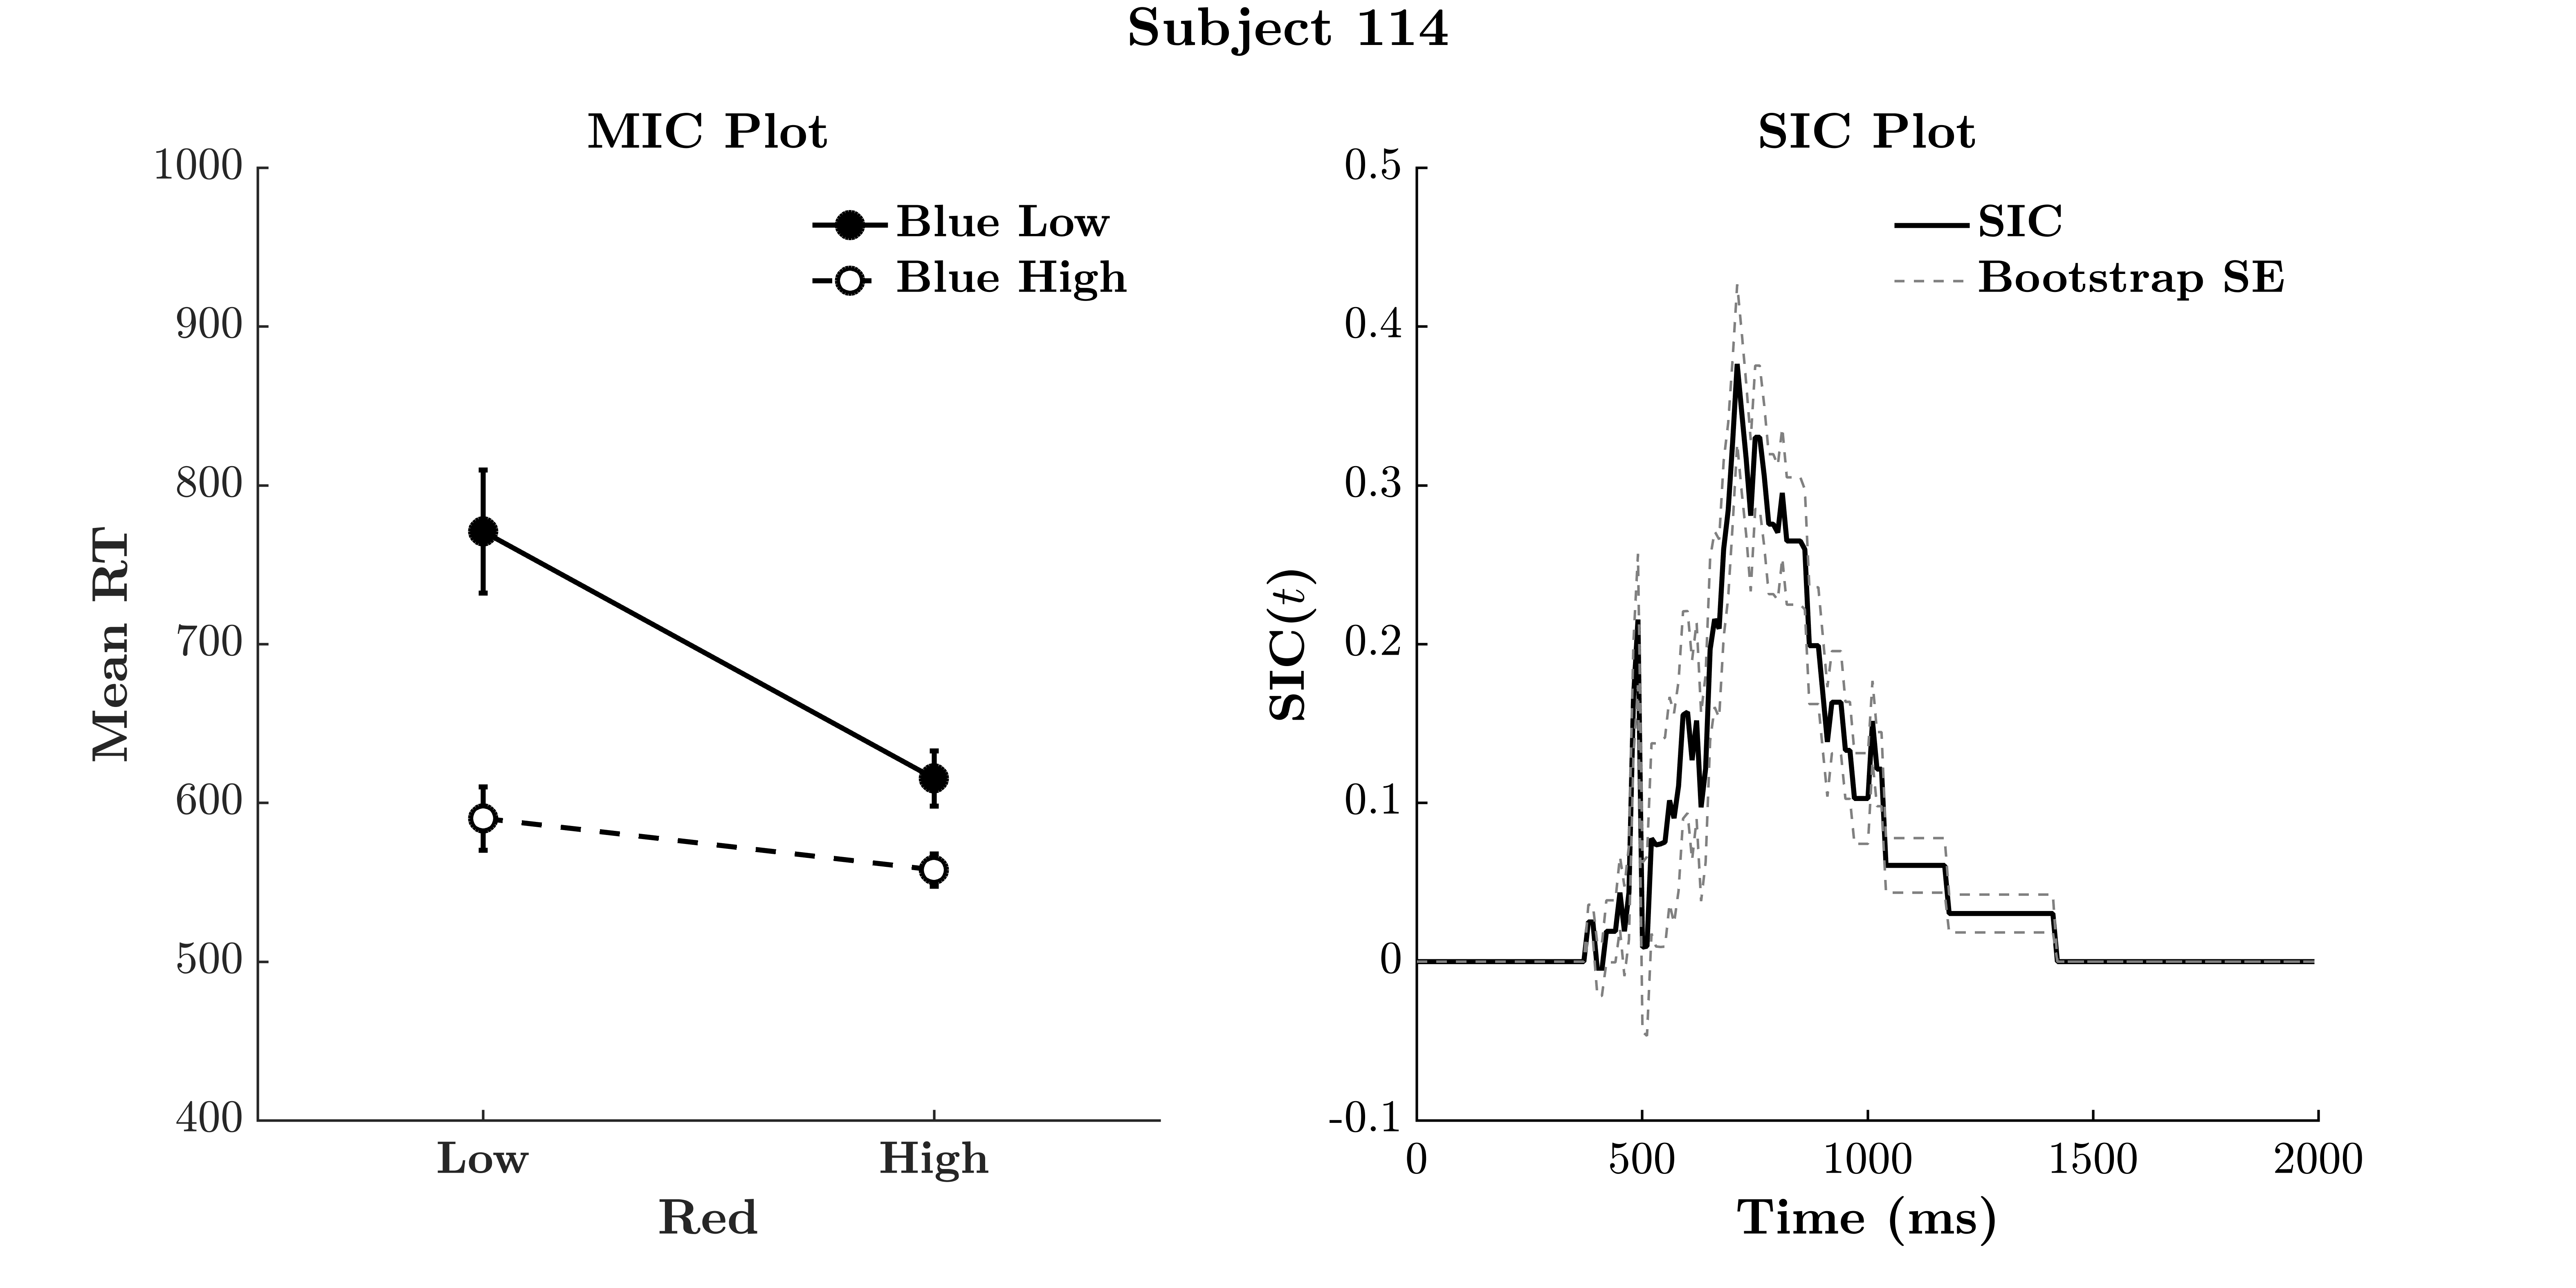
\includegraphics[width=\linewidth]{Figures/EstSystems/FIG11JPG.jpg}
\caption{Illustration of double-target mean interaction contrast (MIC; left) and survivor interaction contrast (SIC; right) plots for subject 114, displaying an over-additive MIC and a parallel minimum-time processing architecture. The MIC plot depicts mean RT for the high and low salience levels within the red and blue target color sets. Error bars represent $\pm$ one standard error of the mean. The presence of a high salience target in either color-set resulted in a fast target-present response, resulting in the illustrated interaction. By contrast, a serial or additive MIC would display no interaction. The SIC plot depicts a positive SIC function across all time points, supporting a parallel minimum-time processing architecture.}
\label{fig:EgSIC}
\end{figure}

\subsubsection{Experiment 2: Fixed Size, Divided Color-Sets}
In Experiments 2--4, processing models were diagnosed in the same way as Experiment 1. A summary of these results are reported next, and the complete results are reported in the supplementary materials S1, Table \ref{table:DT}. SIC classification supported parallel minimum-time processing in three subjects, with model probabilities $> 0.5$, and parallel minimum-time processing in one subject with a model probability $< 0.5$. One subject's data did not display selective influence at the level of the distribution, however, ordering held at the level of the mean. As such, they were subjected to MIC analysis and supported a parallel maximum-time processing architecture, confirmed by visual analysis of the MIC and a significant MIC interaction. Bayes factor analysis of the group posterior MIC provided moderately strong evidence (BF$_{10}$ = 5.11) in favor of a parallel minimum-time architecture. This result replicated in all individuals.

\subsubsection{Experiment 3: Fixed Area, Mixed Color-Sets}
After SIC categorization, three subjects displayed a parallel minimum-time processing architecture with model probabilities greater than 0.5. One subject displayed a parallel minimum-time processing architecture with an inconclusive model probability. One subject was only assessed at the level of the MIC. Bayes factor analysis of the group posterior MIC provided moderate evidence (BF$_{10}$ = 3.42) in favor of a parallel minimum-time processing architecture. This result replicated in three individuals, with two individuals displaying anecdotal evidence (BF$_{10}$ $<$ 3) in favor of parallel minimum-time processing.

\subsubsection{Experiment 4: Fixed Area, Divided Color-Sets}
After SIC classification, one subject displayed a parallel minimum-time processing architecture, and two subjects a parallel maximum-time processing architecture, with model probabilities greater than 0.5. One subject was only assessed at the level of the MIC. Bayes factor analysis of the group posterior MIC provided anecdotal evidence (BF$_{10}$ = 2.68) in favor of a parallel minimum-time processing architecture. This result replicated in two individuals. The remaining subjects provided anecdotal evidence towards a parallel maximum-time processing architecture. 

Overall, MIC and SIC results from trials in which subjects estimated two target sets ($i$.$e$., both red and blue sets had less than 20 discs each), revealed mostly parallel architecture, typically with a minimum time stopping rule (Experiments 1--3), but a maximum time stopping rule in Experiment 4. 

\section{Discussion}
When asked to estimate the quantity of two item-sets and compare them to an internal criteria, participants were able to complete the task quickly and accurately. Across the four experiments, subjects typically displayed a significant redundancy cost, and severe workload capacity limitations when estimating multiple item-sets. This capacity was so limited, as to be slower than our predictions of a theoretical serial estimation system. Workload capacity measured by the resilience function contradicted these finding, supporting an unlimited capacity, parallel estimation system. In each experiment, a limited set of subjects afforded SIC analysis of double-target responses, providing conclusive evidence that two item-sets may be estimated simultaneously through a parallel estimation-system. These results were further supported by hierarchical Bayes factor analysis, displaying moderate evidence for parallel estimation-systems.

In addressing the primary aims of this Chapter, we have determined that comparative estimation systems operate under a parallel system architecture. We determined that this parallel processing system is severely limited in workload capacity to the point that it is less-efficient than a theoretical serial estimation system. Finally, we found that these results were consistent across our conditions of item-set separability and our manipulations of item-set area. The following discussion provides a deeper breakdown on each of these elements.

\subsection{Workload Capacity}
Most subjects in Experiments 1--4 displayed a significant redundancy cost when estimating two target item-sets. This indicates that subjects had limited cognitive resources when performing estimates on multiple item-set. Capacity coefficient analysis confirmed these indications, with all subjects showing limited workload capacity, at or below the Grice lower-bound. The lower-bound is a theoretical approximation of a serial processing system. Therefore, a capacity coefficient residing at this bound indicates the system mean RT could be explained by either a serial model, or a parallel model with limited capacity. Fortunately, these are the exact mimicry conditions the SFT machinery was designed to counteract. When the lower-bound is violated --- as was the case for all subjects --- the system experiences an additional limitation to processing beyond the expectations of a serial model. This indicates the system experiences a violation of item-set $context$ $invariance$.

A parallel architecture --- as found in the current study --- could violate context invariance and yield severely limited capacity through a number of ways. Under one account, processing channels might inhibit each other, acting to slow the rate of processing in the alternate channel. In their investigation of workload, \citeauthor{eidels2011} \citeyear[Figure 3]{eidels2011} illustrated how a parallel minimum-time system with cross-channel inhibition (both pre-accumulation and post-accumulation) can predict severely limited capacity and maintain an all-positive SIC. We term this the inhibition hypothesis. 

An alternative account suggests that the rate of processing (evidence accumulation) in double-target trials is slower than in single-target trials, we term this the rate hypothesis. The rate hypothesis may occur under several conditions: (i) double-target processing-rates may slow with increases to the total stimulus set-size (the sum of red and blue items); (ii) double-target processing-rates may slow due to context effects, for example, crowding effects \cite{anobile2015mechanisms} or figure-ground segmentation effects \cite{kimchi2008figureground}. Or, (iii) double-target processing-rates may slow with the number of component item sub-sets, for example, red, blue, green and yellow item-sets. 

To test the feasibility of the rate hypothesis, we simulated a parallel model with limited capacity at the level of the accumulator using the linear ballistic accumulator (LBA) model \cite{Brown2008}. Figure \ref{fig:LimVsUnlim} illustrates \SIC and \Ct predictions when processing-rates are fixed (top panels), compared to when processing-rates are slower for double-target trials only (bottom panels). Simulated results from the slowed double-target rates, match observations from the current study. Both the inhibition hypothesis and the rate hypothesis can produce an all-positive SIC with severely limited workload capacity. To determine which hypothesis is most likely, we now consider the resilience difference function.

\begin{figure}[hbt]
\centering 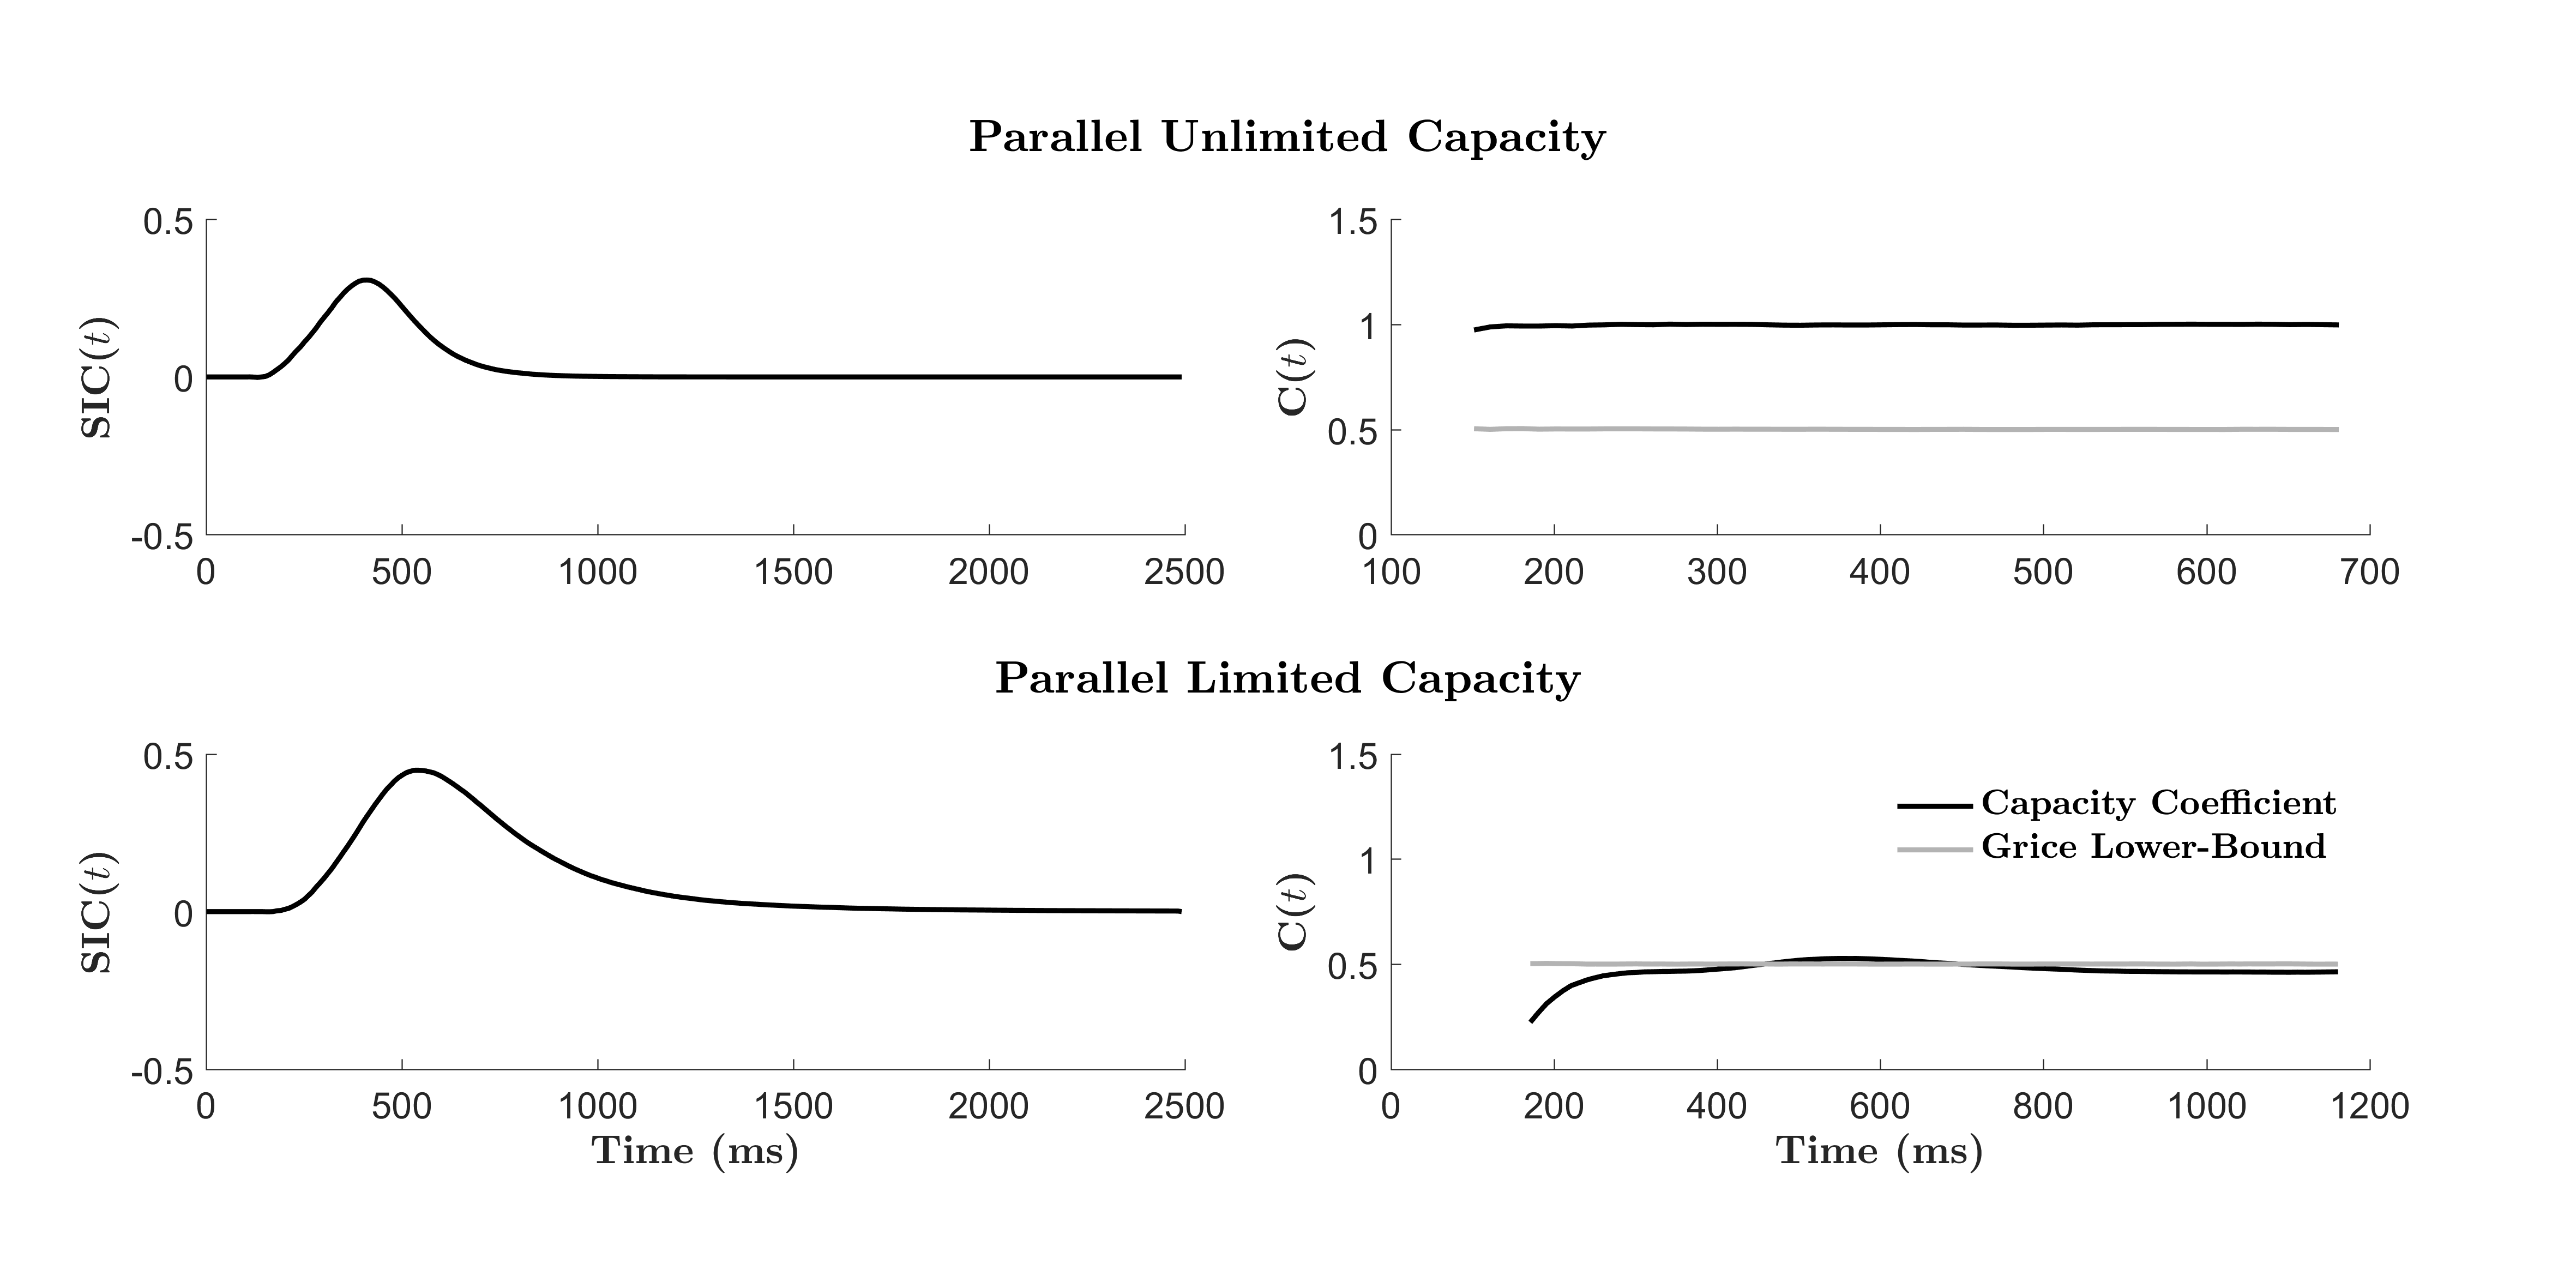
\includegraphics[width=\linewidth]{Figures/EstSystems/FIG12JPG.png}
\caption{Survivor interaction contrast SIC($t$) functions (left) and capacity coefficient C($t$) functions (right) for parallel minimum-time unlimited (top) and limited capacity (bottom) processing systems. Simulations are independent and identically distributed, and were completed with 100'000 trials per trial-type using the LBA. Threshold was set to 3, start-point 2, standard deviation 1 and non-decision time zero. Drift rates were fixed at 7 (high-salience) and 4 (low-salience), except for limited-capacity double-target trials where drift rates were reduced to 5.5 and 2.5, respectively.}
\label{fig:LimVsUnlim}
\end{figure}

\subsection{Resilience}
The resilience difference function compares the response-times for processing two-target item-sets, to the response-times for processing a target and distractor (conflict-target) item-set. Resilience difference factors out the effect of the distractor channel, providing a direct assessment of processing architecture and workload, without altering the number of processing-channels, (i.e., item-sets). Our analysis of resilience matched predictions made by an unlimited capacity, parallel processing architecture. This suggests that target processing was similar between conflict-target and double-target conditions, and that processing channels did not inhibit one another \footnote{Rdifference predictions for the inhibitory parallel model are demonstrated in \cite{Little2018mixmodel}.}. This finding directly contravenes the inhibition hypothesis. Resilience analysis also addresses a secondary question: does comparison to an internal criterion alter workload capacity. As conflict-target trials were assessed through a parallel unlimited-capacity processing system, we conclude that comparisons to an internal criterion do not alter system workload. We now consider the impact of context effects on estimation system workload capacity.

\citeA{goldfarb2013distsubitizing} observed that distractor items which could not be easily grouped, increased sub-set estimation-times. This finding aligns with our results: the presence of a redundant target-set slowed double-target response-times. Prior to this study, \citeA{HALBERDA_2006} revealed that in the presence of distractors the entire item-set was estimated $prior$ to the estimation of each item sub-set, slowing the estimation process. In line with our analyses, these findings suggest a precedence to the system workload \cite<\`a la >{navon1977forest}, with limitations occurring prior to the estimation of each item sub-set. \citeA{goldfarb2013distsubitizing} further revealed that perceptual properties, such as color and item location, were identified prior to sub-set estimation. This allows for potential context effects.

Context effects, such as the crowding effect \cite{anobile2015mechanisms} and the figure-ground segmentation effect \cite{kimchi2008figureground} disrupt single item identification and slow the rate of enumeration. Such effects are most commonly observed in dense visual scenes, for example, when more than one item-set is present. As indicated by \citeA{goldfarb2013distsubitizing}, these effects could occur prior to the enumeration of each item sub-set, slowing double-target responses relative to single-target responses. Although the separation of item-sets in Experiments 2 and 4 could allow participants to ignore the presence of an additional item-set, capacity coefficient analysis suggests this manipulation had no effect. This indicates that the item sub-sets were processed in a similar manner in both mixed and divided item-set conditions. As such, it is possible our observed limitations to workload capacity are a result of context effects occurring prior to the estimation of each item sub-set.

An alternative account of the rate hypothesis assumes that workload is limited due to the total number of items across the item sub-sets. If true, capacity should be less-limited for when the total array size is smaller than when it is larger. A comparison of estimation system workload that was sensitive enough to diagnose this difference was not possible using the current data set. Instead, we will address this account of the rate hypothesis in the following Chapter where we examine the workload capacity and processing architecture of a comparative subitizing system. 

The final condition of the rate hypothesis suggests that capacity may become more limited due to the addition of each item sub-set, for example, a red, blue and green item-set. If the capacity limitations observed in the current analysis did not violate the Grice-bound, this hypothesis could be plausible. However, the Grice-bound violation suggests that the processing of one item-set in some way inhibits the processing of the other. This inhibition requires additional cognitive constraints that go beyond the additive workload imposed by an additional item-set. For example, the context effects that may co-occur with the addition of an item-set. For this reason, any further discussion of the rate hypothesis will focused upon i) the size of the total item-set array, or ii) the impact of context effects. Having discussed our results of workload capacity, we now turn our attention to processing architecture.

\subsection{Processing Architecture}
Only a limited number of subjects met the inclusion criteria for processing architecture. As such, so we discuss results pooled across the four experiments. 

Of the fifteen subjects whose processing architecture could be conclusively assessed at the level of the SIC, all displayed a parallel processing architecture. These results align with previous findings by \citeA{HALBERDA_2006}, who used estimation acuity to theorize the parallel estimation of up to three item-sets. Results from the current study validate this theory for up to two item-sets by applying the diagnostic response-time measures of SFT.

Hierarchical Bayesian MIC analysis, conducted across a wider range of subjects, also provided moderately strong evidence in favor of parallel processing. These findings were observed at both the individual and group posterior level, and across all four experiments.

The current study is the first adaptation of the SFT framework to the study of estimation systems and came with notable limitations. In our assessment of the SIC, three subjects displayed non-determinable double-target processing architectures, and thirty-seven subjects did not meet the necessary requirement of selective influence. This suggests our manipulation of selective influence, (i.e., the numerical distance effect), was not effective for a majority of subjects. 

Through extensive testing (Chapter 2), we determined target and distractor salience levels that would ensure a high-degree of accuracy, and a significant response-time effect. As expected, we observed high accuracy in our primary task, however, our manipulation of response-time did not replicate. We suggest this effect is best explained by context effects, and small trial numbers.

As previously discussed, the presentation of multiple item-sets may have resulted in context effects that slowed item-set estimation. This effect could have compromised our manipulation of salience, leading to a lack of selective influence among the majority of tested subjects. Our manipulation of salience was particularly ineffective when item-set area was controlled, and when item-sets were separated. These manipulations may have inadvertently created a perceptual covariate of quantity, such as item-set density. This would allow subjects to identify target item-sets without engaging the ANS and our manipulation of salience. Alternately, our manipulations may have enhanced the interference produced by context effects. Both of these accounts could equally result in the poor manipulation of target salience observed within a majority of participants. 

A second limitation to our task design was the use of relatively few double-target trials \cite<compared to typical SFT studies c.f.,>{eidels2015evaluating,townsend2011}. Small trial numbers may result in unstable survivor distributions, leading to a poor manipulation of selective influence and unreliable SIC functions. As such, both small trial numbers and the presence of context effects may have contributed to our poor manipulation of salience. 

The current study faced several limitations, however, these limitations did not appear to change the fundamental processing architectures observed between Experiments. Rather, these limitations altered the number of subjects who could be diagnostically classified. As a result, it is impossible to draw strong conclusions regarding the impact of item-set area, or item-set separability, on processing architecture. 

Our findings provide conclusive evidence that double-target item-sets may be estimated through a parallel estimation system. These findings were observed by a majority of subjects whose processing architectures could be categorized. Through the novel application of SFT to an estimation task, we provide a nuanced account of the relationship between processing architecture, workload capacity and stopping-rule. Notably, we observe capacity limitations occurring before sub-set estimation, possibly caused by context effects occurring at the presentation of multiple item-sets.

These results are important, as they provide a rational for why high cognitive workload my be experienced when estimating multiple item-sets. Understanding this limitation to the human estimation system is particularly important for circumstances requiring item-set estimation under extreme or irreducible levels of workload. For example, emergency responders to a scene identifying how many people require attention, or theatre attendees choosing the fastest of two crowded exits under duress of a fire alarm. 

\subsection{Conclusion}
People often need to estimate and compare quantities, be it the number of people in line to the bank teller, party guests, or players in football teams. Little research has investigated the ability to estimate multiple quantities at the same time. Fewer still have applied machinery that can overcome parallel-serial mimicry concerns, and assess the cost to processing multiple item-sets (workload capacity). The current study is the first known attempt to apply SFT to the question of multiple-set estimation. In a series of four experiments, participants were presented with either one or two sets of 10-41 colored discs (red, blue) and had to estimate whether the number of items in each set was smaller or greater than some criterion value. SFT analyses revealed rather sever capacity limitations, meaning there was a toll in processing efficiency when subjects had to estimate the number of items in two sets relative to just one set. These results suggest that while estimation may be colloquially viewed as an effortless and possibly automatic process, the estimation of multiple item-sets is in fact a rather demanding feat. Specifically, estimating two sets was inefficient to the extent it was comparable (in terms of processing capacity) to serial processing. Understanding the fundamental cognitive mechanisms that cause this limitation is of paramount importance if we are to reduce the effective workload experienced by individuals performing multiple item-set estimates. Doing so will afford faster and more accurate estimates under difficult conditions, when we must make quick and informed approximations of quantity. This is a challenge we leave to future research.


\chapter{Subitizing Systems} 

\label{Chapter 4}
\lhead{Chapter 4. \emph{Subitizing systems}}
\vspace{3cm}
\newpage

\section{Chapter Overview}
% Premise
Whether we realise it or not, many everyday comparisons of quantity occur within the subitizing range, 1--4. For example, when we choose the fewer of two coffee queues, we may rapidly subitize each queue before deciding which one to join. As we go to pay, we might empty our wallet of coins and subitize the gold coins from amongst the silver shrapnel. In both of these instances, we are using a subitizing system to evaluate item-sets when those sets are physically separate (e.g., coffee queues) or intermixed (e.g., coins). But under what processing architecture and workload capacity does this subitizing system operate?

In Chapter 3, we found that two item-sets may be estimated at the same time through a parallel estimation system. As speculated by \citeA{HALBERDA_2006}, subitizing systems may also operate under a parallel processing architecture. In the current Chapter, we aim to address this question of processing architecture with empirical data. Using SFT, we will assess the processing architecture of subitizing systems and determine whether subitizing systems operate under a serial or parallel processing architecture.

In the previous Chapter, we found that estimation systems perform under severe constraints to workload capacity. These constraints were such that the observed parallel processing system was less efficient than that of a theoretical serial processing system. In our discussion of estimation system workload, we noted that the number of items in both item sub-sets may influence the capacity of the system. If true, we should expect workload capacity to be less-limited in a subitizing system, than in the previously measured estimation system. 

An alternative explanation suggests that context effects created the severe limitations in estimate system workload capacity. If the presence of an additional item-set violates the assumption of context invariance --- that the presence of one item-set impacts the processing of the other --- we might expect to see similar limitations in workload capacity between subitizing and estimating systems. If so, we should expect subitizing systems to display severe limitations to workload capacity, with the capacity coefficient measuring at or below the Grice lower-bound. 

In this Chapter, we will characterize information-processing approaches for subitizing two colored item-sets (red and blue discs), when comparing these sets to an internal representation of quantity (three or four items). We will develop an extended double-factorial paradigm using quantities within the subitizing range (1--4). Using experimental data, we will apply the machinery of SFT and assess system workload capacity and processing architecture i) when two item-sets are intermixed and ii) when two item-sets are physically separated. By comparing workload capacity between estimation and subitizing systems, we will determine whether system capacity is impacted by i) the number of items in both item sub-sets, or ii) context effects occurring in the presence of an additional item-set. To foreshadow the results of this study, we find subitizing systems operate under severely limited workload capacity and under predominantly serial processing system architectures.


\section{Subitizing processing architecture}
In the earliest academic account of subitizing, \citeA{jevons1871power} described how five or fewer beans might be counted ``at a glance" without cost to accuracy. Later, \citeA{kaufman1949subtizing} coined the term `subitizing', and showed the time to count four or fewer items was comparable, yet the time to count further items increased with set-size. This led \citeA{kaufman1949subtizing} to speculate that subitizing was a holistic process, capable of quantifying an entire item-set simultaneously. Later, \citeA{pylyshyn1988tracking} extended this account with a visual indexing theory, suggesting a pre-attentive visual tracking system limited to four or fewer items. While more recent work has shown subitizing requires attention \cite{Burr2010}, the notion of a parallel indexing system has remained. Today, subitizing is thought to form part of the Object Tracking System \cite<OTS; also known as the parallel individuation system; >{Hyde2011}, and have a four item-limit due to limitations within visual working memory \cite{cowan2001magical, leslie1998indexing}. 

The ability to subitize a group of items through the OTS, affords the potential of a parallel subitizing system. In their description of `groupitizing', \citeA{starkey2014groupitizing} described how an item-set could be enumerated faster, if the items were grouped into subitizable sets. For example, twelve items may be enumerated faster when grouped into three groups of four, or four groups of three. A speed advantage may be observed when groupitizing for one of two reasons.

Groupitizing might reflect the ability to quickly subitize item sub-sets in sequence, and sum or multiply their value by the number of sub-sets. This strategy could be characterized by a serial processing architecture. Alternately, groupitizing might reflect the ability to subitize the value of multiple item sub-sets at the same time. This strategy could be characterized by a parallel processing architecture. Both parallel and serial subitizing systems would predict faster enumeration than the serial counting of each item individually. Diagnosing whether subitizing systems operate in parallel or serial is one aim of the current study. 

\subsection{Subitizing workload capacity}
As previously noted, workload capacity will form an important line of investigation within the current study. In the previous Chapter, we found severely limited workload capacity within parallel estimation systems. This limitation was either due to i) the number of total items in the stimulus array, or ii) the violation of context invariance where the enumeration of one item-set was impaired by the presence of another. If the number of displayed items altered workload capacity, we expect capacity coefficient results to be less-limited in the current investigation. However, if workload was limited due to context effects, we expect workload capacity results to mimic those of the previous Chapter. Specifically, we expect workload capacity to be limited to such a degree, that the capacity coefficient violates the Grice lower-bound. With clear expectations for processing architecture and workload capacity in place, we must now consider the design and quantities that will be used in the current study. 

\subsection{Subitizing targets and distractors}
In Chapter 2, we performed a pilot study to select target and distractor quantities within the range of estimation for use in an expanded double-factorial paradigm. The primary aims of this study were to i) select target quantities that would result in a numerical distance effect on RT, and ii) ensure accurate responses. In the current study, we aim to use an extended double-factorial paradigm to test systems of subitizing. Therefore, targets quantities must be within the range of 1--4. As a result, we expect all responses to be highly accurate as subitizing is characteristically an accurate process.

In the selection of target quantities, a number of considerations must be made. While the subitizing range is generally considered to range from 1--4, this range has been shown to vary from individual to individual \cite<for example,>{green2003action}. As a conservative measure, we will limit our maximum target value to 3. Having defined our maximum target, we must now define our smallest target. 

A single item may be evaluated by the process of subitizing, or by a process of perceptual detection. In the context of an enumeration task, it is likely a single-item will engage the process of subitizing due to the task-context. However, there is a chance participants will associate the detection of a single-item with a target-response, potentially facilitating response-times. As such, conclusions regarding processing architecture and workload should not be limited to when target items include only a single unit, (\eg 1 vs 2, or 1 vs 3). To address this, we will perform two concurrent investigations. In one investigation, we will adopt a criterion of three items; targets will be one-item and two-items. For symmetry to the target sets, distractors will be four-items and five-items. In the second investigation the criterion will be four-items; targets will be two-items and three-items, and distractors will be five-items and six-items. 

Similar to our investigation of estimation systems, we must consider the effect of low-level perceptual covariates on the subitizing system. For this reason, each investigation will control for the effect of item-set area in a similar manner to Chapter 3. This will be completed in conjunction with the manipulation of item-set separation (intermixed vs separate color-sets), within the framework of an extended double-factorial design.


\section{Method}
The method of this study is very similar to that of the previous chapter. For the sake of brevity, only the primary differences will be described. The first factor manipulation of our expanded double-factorial paradigm was the presence or absence of a target item-set. Target-sets were defined as containing fewer than either a criterion of three or four items. Distractor-sets were defined as containing more than the criterion. 

At the second factor level, the salience of each item-set was manipulated relative to the central criterion of three or four items. Salience was manipulated through the numerical distance effect \cite{buckley1974comparisons}; quantities closer to the criterion were harder to evaluate than quantities further away. High-salience targets were defined as being two items fewer than the criterion and low-salience targets were defined as being one item fewer than the criterion. High-salience distractors contained two more items than the criterion and low-salience distractors contained one more item than the criterion.

As in Chapter 3, we applied an expanded double-factorial design across four experiments to assess the impact of spatial separation and low-level perceptual covariates on the subitizing system. Figure \ref{fig:subStim} illustrates the experimental stimuli for a criterion of three, and how they differed across the four factorial manipulations of item-set area and item-set separability (left-to-right, experimental manipulations 1--4; Figure \ref{fig:subStim}).

%The first experimental manipulation assessed subitizing systems when two colored item-sets were intermixed. The second manipulation assessed subitizing systems when item-sets were physically separated. The third manipulation assessed subitizing systems when item-sets were intermixed and item-set area was matched. The final manipulation assessed subitizing systems when item-sets were separated and item-set area was matched.


\begin{figure}[hbt]
\centering \includegraphics[width=\linewidth]{Figures/Subitizing/SubStim.jpg}
\caption{Example stimuli using a criterion less-than three, when discs were of a fixed size (left), and when item-set area was fixed (right); for mixed and separate item-set designs. Each example illustrates a conflict-target response-condition, where one color-set is fewer than three, and one color-set is greater than three.}
\label{fig:subStim}
\end{figure}


\subsection{Participants}
Participants were undergraduate psychology students from the University of Newcastle, Australia, who completed a 90 minute experiment for three course-credits. All participants reported  normal or corrected to normal vision, and intact color vision. The number and mean age of participants in each experiment are displayed in Table \ref{tab:Sub_Participants}.

\begin{table}[htb]
\centering
\caption{Participant number and mean age, for each experiment.}
\begin{tabular}{l l l l l l} 
\hline
Exp & Criterion & \begin{tabular}{l} Perceptual \\ Control \end{tabular} & \begin{tabular}{l} Item-Set \\ Proximity \end{tabular} & \begin{tabular}{l} Participants \\ (Female) \end{tabular}  & Age (SD) \\
\hline
1.1 & 3 &~Fixed Disc Size   &~Mixed     &~9 (5) & 22.67 (8.59) \\
1.2 & 3 &~Fixed Disc Size   &~Separate  &~6 (4) & 26.5 (14.63) \\
1.3 & 3 &~Matched Set Area  &~Mixed     &~9 (6) & 22.67 (6.08) \\
1.4 & 3 &~Matched Set Area  &~Separate  &~5 (3) & 22.6 (2.07) \\
\hline
2.1 & 4 &~Fixed Disc Size   &~Mixed     &~8 (4) & 22 (3.3)  \\
2.2 &4 &~Fixed Disc Size   &~Separate  &~10 (6) & 20 (1.87) \\
2.3 &4 &~Matched Set Area  &~Mixed     &~8 (6) & 24 (5.04)  \\
2.4 &4 &~Matched Set Area  &~Separate  &~8 (5) & 23.89 (5.58)  \\
\hline
\hline
\label{tab:Sub_Participants}
\end{tabular} 
\end{table}

\subsection{Stimuli and apparatus}
The testing facilities and stimulus properties, (e.g., color, presentation), were identical to those used in Chapter 3. In the first experimental manipulation, the size of each disc was fixed and item-sets were intermixed. In the second experimental manipulation, the size of each disc was fixed, however, item-sets were confined to the top or bottom hemisphere of the central circular field-of-view. In the third experimental manipulation, item-sets were intermixed, and the size (radius) of each item varied. On each trial, the \textit{total} areas of the red and blue color-sets were matched. Color-set area was randomly sampled at the start of each trial and varied within a range of 74-222 pixels, and 98--294 pixels, for criterion three and four respectively. The final experimental manipulation matched item-set area (as previously described), and presented item-sets in either the top or bottom hemispheres of the central circular field-of-view (see Figure \ref{fig:subStim}). 

\subsection{Procedure}
The procedure of this experiment matched that of the previous Chapter, with the addition that participants were randomly allocated to either a criterion three or criterion four task, and to one of the four factorial manipulations of item-set area and item-set separability. 

% Each participant completed a single 90 minute experimental session and were randomly allocated to a criterion 3 or criterion 4 task. Participants were presented with an information sheet and consent form, and answered demographic questions regarding age, gender, handedness, vision and color-blindness. Participants were asked to complete a redundant-target subitizing task, in which any display containing a target set (number of discs in set $<$ 3 or $<$ 4, depending on allocation) called for a `yes', target-present response. Any display containing only distractor item-sets (e.g., a double-distractor or a single-distractor only item-set), called for a `no', target-absent response. Participants responded `yes' to the presence of a target with the `z' key and `no' to the absence of a target with the `/' key. Response keys were counter-balanced across participants.

% At the start of each trial, participants were directed to look at a central fixation cross, presented for 500ms and followed by a 500ms blank screen. The stimulus display was then presented for 500ms, followed by a mask for 500ms and a post-mask blank for 3000ms. From the onset of the stimulus, participants had 4000ms to make a response. The trial ended when the participant made a response or the trial timed-out at the conclusion of the response window. Note that a 500ms stimulus display was used in this task. Subitizing is a rapid enumeration process, and a longer display time might encourage participants to count, rather than subitize each item-set.

% Participants completed one practice block and 15 experimental blocks, each containing 96 randomly ordered trials. Trial-by-trial accuracy feedback was provided during the practice block. Each block contained 12 double-target trials, 12 double-distractor trials, 24 conflict-target trials, 24 single-target trials and 24 single-distractor trials, presented in a random order. These trials were evenly distributed among the constituent salience levels. For example, three trials were presented from each double-target salience combination --- 12 in total. By comparison, six trials were presented from each of the red and the blue, single-target high and single-target low salience conditions --- 24 in total. Not including practice trials, each subject completed 180 double-target trials, 180 double-distractor trials, 360 conflict-target trials (180 target-red, 180 target-blue), 360 single-target trials (180 target-red, 180 target-blue) and 360 single-distractor trials (180 distractor-red, 180 distractor-blue). In total, subjects completed 1440 experimental trials with a 5:3 yes/no response bias. The probability of a target item-set in one color (e.g., red), given a target item-set in the other color (e.g., blue), was 0.33 \cite{mordkoff1991}.

\section{Data analysis}
Incorrect trials, and trials with response times less than 150 ms or greater than the 97.5$^{th}$ percentile were excluded from analysis. Participants' data were included if their total accuracy was $>80\%$ correct, \emph{and} their conditional accuracy in each of the six target conditions was $>66\%$. All repeated-measures ANOVAs were corrected for violations of sphericity, where appropriate, using the Greenhouse-Geisser correction. Post-hoc paired $t$-tests were corrected for family wise error using the Bonferroni method. As in the previous Chapter, workload capacity was assessed through the redundant target effect \cite<RTE; >{miller1982divided, eidels2008similarity}, capacity coefficient and resilience difference function. Processing architecture was assessed for double-target conditions using the MIC and SIC($t$). Selective influence between the double-target salience conditions was assessed for each subject using a series of non-parametric KS tests at an alpha $p <$ .15 \cite{johnson2010systems}. 

\color{\Red}
\section{Results}
\subsection{Accuracy}
Participants with conditional accuracy $< 66\%$ or total accuracy $< 80\%$ were excluded from analysis. Thirteen participants were excluded across all experiments, displayed separately for each experiment in Table \ref{tab:Sub_Acc}. Accuracy was high for the remaining participants across experiments ($M$ = .91, $SD$ = 0.04). The rest of the analysis will focus exclusively on assessments of response-time.

\begin{table}[htb]
\centering
\caption{Participant exclusions and mean accuracy in each experiment.}
\begin{tabular}{ l l l l l l } 
\hline
Exp & Criterion & 
\begin{tabular}{l}Perceptual \\Control \end{tabular} & \begin{tabular}{l}Item-Set \\Proximity \end{tabular} & Excluded N & \begin{tabular}{l}Mean \\Accuracy (SD) \end{tabular} \\
\hline
1.1 & 3 &~Fixed Disc Size   &~Mixed     & 1  &~.92 (.05) \\
1.2 & 3 &~Fixed Disc Size   &~Separate  & 0  &~.94 (.02) \\
1.3 & 3 &~Matched Set Area  &~Mixed     & 1  &~.92 (.05) \\
1.4 & 3 &~Matched Set Area  &~Separate  & 1  &~.90 (.06) \\
\hline
2.1 & 4 &~Fixed Disc Size   &~Mixed     & 3 &~.90 (.02)  \\
2.2 & 4 &~Fixed Disc Size   &~Separate  & 2 &~.89 (.01) \\
2.3 & 4 &~Matched Set Area  &~Mixed     & 4 &~.92 (.03)  \\
2.4 & 4 &~Matched Set Area  &~Separate  & 1 &~.90 (.05)  \\
\hline
\hline
\label{tab:Sub_Acc}
\end{tabular} 
\end{table}

\subsection{Target mean RT}
The following section focuses on %AE: focuses ON,  not UPON (though grammatically correct)
our conditions of load: the double-target (Dt), red single-target (Rt), and blue single-target (Bt) conditions. These response-sets are formed from the combination of their nested salience levels. For example, red single-target responses are the aggregate pool of all high (H) and low (L) red target-salience trials, and double-target responses include combinations of HH, HL, LH and LL red-and-blue target-salience levels.

Mean response-time (mRT) results for all experiments are plotted in Figure \ref{fig:subMeanRT}. In each experimental manipulation, regardless of criterion, double-target responses tended to be slower than either single-target red or single-target blue responses. Comparing single- vs double-target conditions, there was a significant effect of workload (number of targets) on response-time, summarized in Table \ref{tab:Sub_ANOVA}. Paired sample $t$-tests were conducted to explore these differences further (fully reported in the supplementary materials, Table \ref{tab:Sub_ttests}). 

%AE: paul, you have used the term 'within target-conditions ' a couple of times above, which i have found a bit confusing, and replaced. consider my suggestion and implement for the rest of the text if you see fit

As seen in Figure \ref{fig:subMeanRT}, double-target responses were significantly slower ($p <$ .05) than at-least-one single-target response condition, in all except two experimental manipulations. There was no significant response-time difference between single- vs double-target conditions when the criterion was three, item-set area was fixed and item-sets were separated. Similarly, here was no significant response-time difference between single- vs double-target conditions when the criterion was four, item-size was fixed, and item-sets were intermixed. No significant response-time differences were observed between red and blue single-target responses, regardless of criterion or experimental manipulation. Overall, these results suggest participants experienced a \textit{redundancy cost} when subitizing two target item-sets. For further insight, we also consider the effects of redundant targets at the individual level.

\begin{figure}[hbt]
\centering \includegraphics[width=\linewidth]{Figures/Subitizing/MeanRTsig.jpg}
\caption{Mean response-time for double-target (Dt), red single-target (Rt) and blue single-target (Bt) conditions, when the criterion was three (top) or four (bottom), and when item-size was fixed (left), and when item-set area was fixed (right). Black markers indicate mixed item-set conditions, white markers indicate separated item-set conditions. Error bars indicate the standard error of the mean. Bonferroni corrected, paired $t$-test significance: * $p <$ .05, * $p <$ .01, * $p <$ .001. }
\label{fig:subMeanRT}
\end{figure}

\begin{table}[htb]
\centering
\caption{Repeated-measures ANOVA results for assessments of target workload in each experiment.}
\begin{tabular}{ l l l l l} 
\hline
Exp & Description & $F$ (df) & Sig & $\eta_{p}^{2}$ \\
\hline
1.1 & Crit 3; Fixed Size; Mixed & 14.93 (2,14)  & $<$ .001 & 0.68  \\
1.2 & Crit 3; Fixed Size; Separate & 5.846 (2,10)  & $<$ .05 & 0.54\\
1.3 & Crit 3; Fixed Area; Mixed & 20.67 (2,14)  & $<$ .001 & 0.75 \\
1.4 & Crit 3; Fixed Area; Separate & 5.353 (2,6)  & $<$ .05 & 0.64 \\
\hline
2.1 & Crit 4; Fixed Size; Mixed & 11.57 (2,8)  & $<$ .01 & 0.74  \\
2.2 & Crit 4; Fixed Size; Separate & 102.9 (2,14)  & $<$ .001 & 0.94\\
2.3 & Crit 4; Fixed Area; Mixed & 59.14 (2,6)  & $<$ .001 & 0.95 \\
2.4 & Crit 4; Fixed Area; Separate & 44.26 (2,7.8)$^+$  & $<$ .001 & 0.86 \\
\hline
\hline
\multicolumn{4}{l}{$^+$ Greenhouse geisser corrected.}
\label{tab:Sub_ANOVA}
\end{tabular} 
\end{table}

\subsection{Redundant target effect}
Figure \ref{fig:subRTE} displays the mean redundant target costs for each subject, broken down by criterion and experimental manipulation. As shown, every participant experienced a redundancy cost (negative RTE), regardless of criterion or manipulation. All individual redundancy costs were significant, measured at the distributional level using a KS alpha $<$ .15. This suggests the addition of a second target slows the subitizing-system, a hallmark of limited capacity processing.


\begin{figure}[hbt]
\centering \includegraphics[width=\linewidth]{Figures/Subitizing/RTE.jpeg}
\caption{Redundant target costs, displayed as separate markers for each individual. All redundancy costs were significant at the distributional level, KS alpha $<$ .15.}
\label{fig:subRTE}
\end{figure}

Redundancy costs were, on average, greater when the criterion was four than when it was three. This may indicate i) an interaction between workload and criteria, ii) a simple effect of criteria on workload, or iii) a proportional increase across all RTs for the criterion four conditions, (\ie a global redundancy cost caused by an overall increase in RT).

To assess whether redundancy costs changed differentially, (\ie interacted), with criteria, several two-way between-subjects ANOVAs were conducted. When item-size was fixed and item-sets were intermixed, there was no main effect of load, (\ie double-target mean RT vs the fastest single-target mean RT; \Fval{1}{22}{4.18}{= 0.05}, $\eta^2$ = 0.16), and no main effect of criteria (\Fval{1}{22}{0.332}{= 0.57}, $\eta^2$ = 0.01). No interaction effect between criteria and load was observed (\Fval{1}{22}{0.474}{= 0.5}, $\eta^2$ = 0.02). Similarly, when item-size was fixed and item-sets were separate, there was no effect of load (\Fval{1}{24}{4.209}{= 0.05}, $\eta^2$ = 0.14), and no effect of criteria (\Fval{1}{24}{0.982}{= 0.33}, $\eta^2$ = 0.03). No interaction effect was observed between criteria and load (\Fval{1}{24}{0.559}{= 0.46}, $\eta^2$ = 0.02). 

When area was fixed and item-sets were mixed, there was a main effect of load (\Fval{1}{20}{6.941}{$<$ 0.05}, $\eta^2$ = 0.2), and a main effect of criteria (\Fval{1}{20}{7.236}{$<$ 0.05}, $\eta^2$ = 0.2). No interaction effect was observed between criteria and load (\Fval{1}{20}{1.377}{= 0.25}, $\eta^2$ = 0.04). Finally, when area was fixed and item-sets were separate, there was no main effect of load (\Fval{1}{20}{1.692}{= 0.21}, $\eta^2$ = 0.05), and a main effect of criteria (\Fval{1}{20}{11.313}{$<$ 0.01}, $\eta^2$ = 0.34). No interaction effect was observed between criteria and load (\Fval{1}{20}{0.166}{= 0.68}, $\eta^2$ = 0.01).

Independent samples $t$-tests were conducted to assess the effect of criteria on the redundancy cost. When item-size was fixed and item-sets were mixed, redundancy costs did not significantly differ between criteria three (M = -49ms, SD = 25ms) and four (M = -97ms, SD = 58ms; \tval{-.679}{10}{= .51}). When item-size was fixed and item-sets were separate, redundancy costs significantly increased from criterion three (M = -37ms, SD = 11ms) to four (M = -78ms, SD = 15ms; \tval{2.559}{9}{$<$ .05}).

When area was fixed and item-sets were mixed, redundancy costs significantly increased from criterion three (M = -29ms, SD = 12ms) to four (M = -75, SD = 12ms; \tval{7.199}{14}{$<$ .001}). Finally, when area was fixed and item-sets were separate, redundancy costs significantly increased from criterion three (M = -39ms, SD = 18ms) to four (M = -74ms, SD = 25ms; \tval{3.388}{6}{$<$ .05}).

Finally, to assess whether the observed increase in redundancy costs were due to an overall proportional increase in RT between criterion three and four trials, we replicated the above analysis with log$_{10}$ transformed response-times. All of the above effects held with log RT, indicating the effects were not caused by an overall or proportional increase in RT between the criteria. 

%%AE1: < sign does not seem to compile properly. AE2: the above section is a bit much, dot you think it is a tad long? in any event, leave it as is for now, not worth investing time to modify...
Results from the RTE and redundancy cost analyses indicate that workload significantly increased with criteria in three of the four manipulations. This effect was not explained by a global increase in response-times, or an interaction effect of response-time and load. It might be that a different cognitive process is occurring when the criterion was three, as to when the criterion was four. The nature of this process is yet unclear. %AE: discard >>These results are interesting and provide a clear comparison between criteria at the level of the mean. 
For further interpretation of individual subject's workload capacity over the entire response-time range, we now turn to the capacity coefficient analysis.

\subsection{Capacity coefficient}
The capacity coefficient allows clear interpretation of performance limitations, compared to an established benchmark UCIP model. Figure \ref{fig:subCap} displays group mean and individual capacity coefficient [C($t$)] results, for each criterion, and each experimental manipulation. In line with the previous redundancy costs, capacity coefficients display limited workload capacity, C($t$) $<$ 1, at both the group (black line) and individual (grey markers) level. Furthermore, each plot depicts \Ct hovering below the Grice lower-bound (broken line) for most of the response-time range\footnote{Late or early crossings of the Grice lower-bound do not reflect a sudden change in workload capacity. Rather, this indicates where the response-time range is poorly defined, (\ie where there are too few double-target responses to make a stable estimate.)}. Individual low-bounds present at approximately \Ct = 0.5, with all individual \Ct scores resting at or below the low-bound for the majority of the response-time range (individual \Ct plots for each experiment can be found in the supplementary materials, Figure \ref{fig:AppB_subCap1} -- Figure \ref{fig:AppB_subCap4}). These results suggest most individuals experienced severe capacity limitations when estimating multiple item-sets.

Analysis of the capacity coefficient and RTE show all subjects subitized multiple target-sets with limited workload capacity. Furthermore, performance of most subjects was below the Grice lower-bound, suggesting they experienced limitations typically associated with a serial processing system. Interpretation of processing architecture and workload capacity, can be extended with our next measure, the resilience difference function. 

\begin{figure}[hbt]
\centering \includegraphics[width=\linewidth]{Figures/Subitizing/SubCapacity.jpeg}
\caption{Capacity coefficient (C($t$)) plots for target-present responses. Group mean \Ct is plotted in black with the Grice lower-bound, an estimate of severe capacity limitations, depicted by the dashed line. Individual participant \Ct values are illustrated by gray markers and mostly fall at or below the group Grice bound, indicating severe capacity limitations across all experimental manipulations.}
\label{fig:subCap}
\end{figure}

\subsection{Resilience difference function}
Resilience difference (R$_{diff}$($t$)) values for the group mean as well as individual subjects, for high target-salience trials, are plotted in Figure \ref{fig:subRdiffHigh}. Interpretation of these results can be aided by comparison to \Rd predictions, presented previously in Figure \ref{fig:Rd}. In all cases, \Rd hovers around zero, for most of the response-time range. While these \Rd functions are far less stable than those observed within the range of estimation, in general, these findings align with the predictions of a parallel minimum-time unlimited-capacity processing system (\Rd = 0). Similar results were displayed by \Rd functions when target salience was low (see Figure \ref{fig:subRdifflow}). While \Rd provides some insight into processing architecture for conflict-target conditions, further interpretation of target architecture requires analysis of the mean and survivor interaction contrasts.

\begin{figure}[hbt]
\centering \includegraphics[width=\linewidth]{Figures/Subitizing/SubRdiffHigh.jpeg}
\caption{Resilience difference plots for when target salience was high and the criterion was three or four, for each experimental manipulation. Black lines depict the average resilience difference function across subjects, while grey markers illustrate individual subject’s resilience difference functions. Average plots show a trend towards \Rd = 0, supporting predictions made by an unlimited-capacity parallel minimum-time processing system.}
\label{fig:subRdiffHigh}
\end{figure}

\begin{figure}[hbt]
\centering \includegraphics[width=\linewidth]{Figures/Subitizing/SubRdiffLow.jpeg}
\caption{Resilience difference plots for when target salience was low and the criterion was three or four, for each experimental manipulation. Black lines depict the average resilience difference function across subjects, while grey markers illustrate individual subject’s resilience difference functions. Average plots show a trend towards \Rd = 0, supporting predictions made by an unlimited-capacity parallel minimum-time processing system.}
\label{fig:subRdifflow}
\end{figure}

\subsection{Double-target processing architecture}
In the following section, we will report the MIC and SIC, as calculated from the response-time differences between double-target salience manipulations --- high-high (HH), high-low (HL), low-high (LH) and low-low (LL). Valid interpretation of the mean interaction contrast (MIC) requires two basic assumptions. The MIC requires selective influence, which is often gauged empirically via the successful manipulation of salience within both target color-sets (determined by the main effects of a between-subjects ANOVA), and correct ordering of the salience conditions, (\ie mRT$_{HH}$ $\leq$ mRT$_{HL}$, mRT$_{LH}$ $\leq$ mRT$_{LL}$). For the MIC, a statistical interaction between the salience levels of each color-set acts as a test for parallel processing architectures, and thus will also be reported. The SIC($t$), in addition to the previous assumptions, requires the assumption of selective influence to hold at the level of the survivor functions, (\ie S($t$)$_{HH}$ $\leq$ S($t$)$_{HL}$, S($t$)$_{LH}$ $\leq$ S($t$)$_{LL}$). Reported MIC and SIC results are limited to those subjects who met the necessary criteria for valid interpretation. 

%AE: above, sign should be equal or smaller than (not just smaller than) -- same fr SIC below. Also, the actual assumption is selective influence, the salience effects and ordering are the empirical test
% PG: Thanks for catching this! 

In the previous Chapter, we classified participant processing architecture using the newly developed non-parametric Bayesian SIC assessment technique, provided by \citeA{houpt2017bayesSIC}. Across all tested participants, only ten met the necessary assumptions for SIC analysis; however, many participants met the assumptions for MIC analysis. As such, results focus on %AE: c'ommon -- upon 
the MIC, and were applicable, are supplemented by SIC interpretations. As in the previous Chapter, processing architecture classification was aided by the hierarchical Bayesian MIC analysis, developed by \citeA{houpt2017hierarchical}. This analysis takes into account data across all valid participants in each experiment. We enhance these results with classical MIC and SIC diagnostic techniques, including visual inspection of individual MIC and SIC plots, and statistical tests for parallel processing architectures. For clarity of exposition, we first summarize the results of classified subjects across all experiments, then present a breakdown by individual subjects. 

\subsubsection{Summary of architectures}
The left panel of Figure \ref{fig:subArchSummary} shows the range of MIC values for subjects who met SIC and MIC inclusion criteria in each experimental type, collapsed across criteria. The majority of subjects in each experiment recorded a positive MIC value, supporting parallel minimum-time processing architectures. Yet, error bars extend to the zero MIC and median MIC values hover near zero, allowing the possibility of serial processing systems. The right panel of Figure \ref{fig:subArchSummary} shows the proportion of processing architectures in each experiment, after classification. Classification reflects the combination of visual and statistical inspection of the MIC and SIC, and hierarchical Bayesian MIC analysis. Each bar represents the total number of classified subjects in each experiment (N reported below each bar), with the shaded regions marking the relative proportion of subjects based on the way they enumerate two target sets (in parallel or serial). When item-set area was fixed and item-sets were separated, the majority of participants displayed a parallel processing architecture. In all other experimental conditions, the majority of subjects displayed serial processing architectures. For simplicity, summary results were collapsed to the serial and parallel categories, across minimum-time and maximum-time stopping-rules. The next section presents individual processing architecture and stopping-rule results. 

\begin{figure}[hbt]
\centering 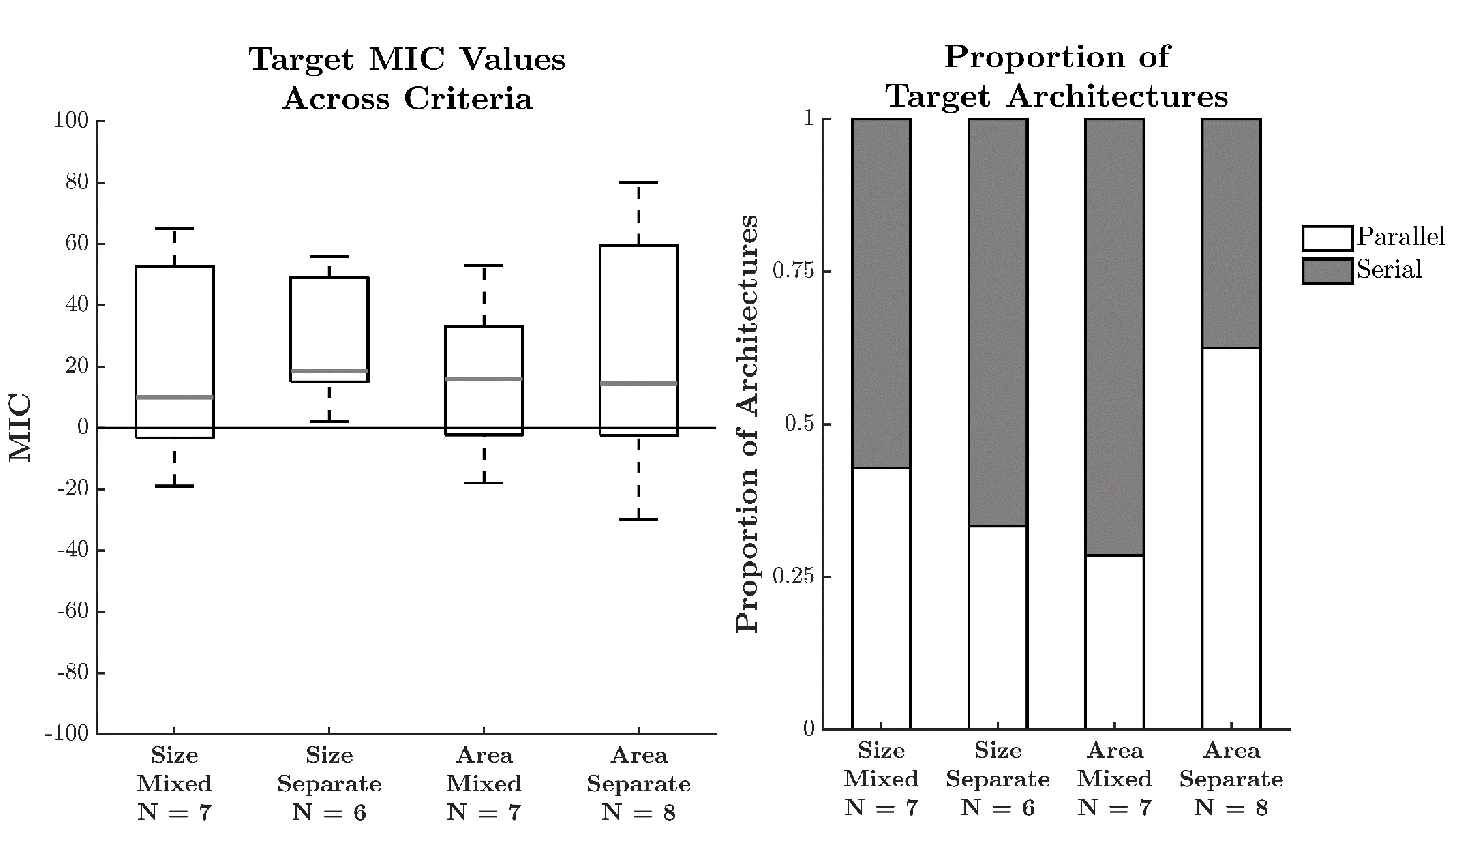
\includegraphics[width=\linewidth]{Figures/Subitizing/ArchSummary3v2.pdf}
\caption{MIC values (left) and the proportion of categorized processing architectures (right) collapsed across criteria. Proportions are relative to the total number of subjects who could be classified using MIC and SIC significance testing. For simplicity, classified architectures have been displayed without stopping-rule.}
\label{fig:subArchSummary}
\end{figure}

\subsubsection{MIC plots}
In the previous Chapter, we noted that the classification of processing architecture can be aided by interpretation of MIC plots. Figure \ref{fig:subMIC1} displays the MIC plots for three participants, when the criterion was less-than three, item-size was fixed and item-sets were mixed. Within ecah panel, each marker denotes a combination of red-target and blue-target salience --- HH, HL, LH and LL. Focusing on %upon 
participant SM 304 (left panel), the MIC value is not significantly different than zero, mean RTs are ordered appropriately, and no interaction of high and low target-salience is apparent in the plot (denoted by the parallel lines and no significant ANOVA interaction). Participant SM 306 follows a similar account; both subjects display results consistent with a serial processing architecture. By contrast, participant SM 308 shows a negative MIC value (-19) with a significant, under-additive interaction term. This interaction is consistent with a parallel exhaustive (maximum-time) processing architecture. Remaining MIC plots for each participant may be found in supplementary materials, Figure \ref{fig:AppB_MIC1} and Figure \ref{fig:AppB_MIC2}. We will summarize these results shortly in Table \ref{tab:subArch}. Processing architecture and stopping-rule classification can be further aided by our next analysis tool, the SIC. 

\begin{figure}[hbt]
\centering 
\includegraphics[width=\linewidth]{Figures/Subitizing/SubMIC.jpg}
\caption{Mean interaction contrast plots for three subjects when the criterion was three, item-size was fixed and item-sets were mixed. The left and middle panel display MIC signatures in line with predictions of a serial (additive) processing architecture. The right panel displays an MIC signature in line with an under-additive MIC signature (parallel maximum-time). * denotes a significant ANOVA interaction, a hallmark of parallel processing architectures. Error bars represent $\pm$ one standard-error of the mean.}
\label{fig:subMIC1}
\end{figure}


\subsubsection{SIC plots}
Figure \ref{fig:subSIC} displays individual SIC($t$) plots, for all participants who met the assumptions of selective influence (at KS alpha $<$ .15) required for valid interpretation. To aid SIC($t$) interpretation, each plot has been augmented with statistical tests \cite{houpt2010statSIC} denoting a significant positive (D+) or negative (D-) deviation from a zero SIC. Recall that a parallel minimum-time processing architecture predicts an all positive SIC($t$), a parallel maximum-time processing architecture predicts an all negative SIC($t$), and a serial maximum-time architecture predicts an SIC($t$) that transitions from negative-to-positive with an MIC = 0. 

\begin{figure}[hbt]
\centering \includegraphics[width=\linewidth]{Figures/Subitizing/SubSIC.jpeg}
\caption{Individual participant SIC($t$) functions, across criteria and experimental manipulations. The black line illustrates the SIC($t$) function, and the dashed line $\pm$1 standard error. Significant positive or negative SIC($t$) deviance from zero are denoted by D$\pm$. Significant MIC interaction terms, indicative of a parallel processing system, are denoted by an *. SM - fixed Size, Mixed item-sets; SS - fixed Size, Separate item-sets, AM - fixed Area, Mixed item-sets. Criterion three experiments are further separated by missing planels.}
\label{fig:subSIC}
\end{figure}

%%AE: figure looks a bit odd -- why are there missing panels ?
% PG: It separates Criterion 3 experiments, added to caption.

The previous MIC signatures of participants SM 304, SM 306 and SM 308 were aligned with a serial, serial and parallel minimum-time processing architecture, respectively. The top three panels of Figure \ref{fig:subSIC} display the SIC($t$) of these three subjects. The SIC($t$) signatures of SM 304 and SM 306 transition from negative-to-positive with a negative deviation (D-), typical of a serial maximum-time processing architecture. These signatures do not display a significant positive deviation (D+), yet, given the MIC is near zero and there is no interaction between target-salience, a serial exhaustive processing system is the most plausible classification. Returning now to the parallel maximum-time MIC signature of SM 308. As predicted by a parallel maximum-time processing architecture, SM 308 displays a negative SIC($t$), and significant negative deviation (D-). Finally, as an example of parallel minimum-time processing, consider participant SS 304. SS 304 displays a positive SIC($t$) function with a significant deviation (D+), a positive MIC and significant MIC interaction. These properties fit precisely with predictions of a parallel minimum-time processing system. Using similar classification methods to those described here, processing architectures have been classified using the MIC and SIC for every individual and are summarized in Table \ref{tab:subArch}. To finalize our analysis, we may now consider our last metric, the hierarchical MIC.

\subsubsection{Hierarchical MIC results}
Table \ref{tab:subArch} summarizes the results of all processing architecture analyses, for each participant. From left-to-right, the table displays the participant ID, the MIC value (and interaction significance *), hierarchical MIC Bayes factor values (\textsubscript{H}BF$_{10}$) for the best fitting processing model (\textsubscript{H}MIC), model categorization of the MIC plot, and model categorization of the SIC plot. Group posterior Bayes factors and associated model categorizations are also reported for each experiment\footnote{Hierarchical MIC analysis was also conducted by collapsing across criteria within each experimental manipulation, however, these results were less informative than the results of the presented table. Differences between the response-time distributions of each criterion, in addition to low participant numbers, produced poorer model fits and Bayes factors close to zero for most individuals.}. To interpret the hierarchical MIC Bayes factor results, we follow the classification scheme of \citeA{lee2014bayesian}, adjusted from \citeA[Appendix B]{jeffreys1961theory}. At the individual and group level, Bayes factors for the best fitting processing model tended towards anecdotal evidence (BF$_{10}$ $<$ 3). In these instances, processing model classification was based on the MIC and SIC plots (as previously described). Where Bayes factors provided moderate evidence towards a single processing model (BF$_{10}$ $<$ 5), hierarchical classifications aligned with the MIC and SIC plot classifications. For ease of exposition, the `winning' processing model classification for each participant is displayed in bold font, in the column denoting how processing architecture was best classified. These processing models were used to create the previous summary in Figure \ref{fig:subArchSummary}. Note that the MIC and hierarchical MIC could not identify the stopping-rule of serial processing architectures.

\clearpage
\begin{table}[!htb]
\caption{Table of individual double-target MIC and SIC results across criteria (subject ID 300 vs 400). The winning model categorization for each subject is displayed in bold font. From left to right, participant ID, MIC value and interaction significance (*), Bayes factor values from the hierarchical MIC analysis and associated MIC model (Parallel: P; Serial S), MIC plot model categorization, and SIC plot model categorization. MIC significance tests conducted at * $<$ .33, ** $<$ .05 and *** $<$ .01. Subject ID abbreviations, SM - fixed Size, Mixed sets; SS fixed Size, Separate sets; AM - fixed Area, Mixed sets; AS - fixed Area, Separate sets.}
\centering 
\begin{tabular*}{\textwidth}{l @{\extracolsep{\fill}} rlllll}
\hline
\textbf{Sub  } & \textbf{MIC} & \textbf{\textsubscript{H}BF$_{10}$} & \textbf{\textsubscript{H}MIC Model}  & \textbf{MIC Plot} & \textbf{SIC Plot}\\  
\hline
SM 304  & -6  & 2.23 & Serial & Serial & \textbf{S Max-Time} \\ % S 4.35
SM 306  & 5  & 2.33 & Serial  & Serial & \textbf{S Max-Time} \\ % S 4.34
SM 308  & -19*  & 2.33 & Serial  & P Max-Time & \textbf{P Max-Time} \\ % S 2.57
\multicolumn{2}{r}{Group Posterior} & 1.5 & Serial & ~ & ~\\
\hline
SS 304  & 49*  & 4.32 & P Min-Time  & P Min-Time & \textbf{ P Min-Time} \\ % S 1.3
SS 305  & 15  & 2.9 & P Min-Time  & \textbf{Serial} & \textbf{ - } \\
\multicolumn{2}{r}{Group Posterior} & 2.88 & P Min-Time & ~ & ~ \\
\hline
AM 301  & 9  & 2.13 & Serial  & \textbf{Serial} & \textbf{ - } \\
AM 302  & 16  & 1.44 & Serial  & \textbf{Serial} & \textbf{ - } \\
AM 304  & 34*  & 1.84 & P Min-Time  & \textbf{P Min-Time} & \textbf{ - } \\
AM 305  & 30  & 1.63 & Serial  & Serial & \textbf{S Max-Time} \\
AM 306  & -6  & 1.94 & Serial  & \textbf{Serial} & \textbf{ - } \\
AM 307  & -18  & 1.86 & Serial  & \textbf{Serial} & \textbf{ - } \\
AM 308  & 53*  & 1.84 & P Min-Time  & P Min-Time & \textbf{P Min-Time} \\
\multicolumn{2}{r}{Group Posterior} & 1.18 & Serial & ~ & ~ \\
\hline
AS 301  & 29*  & 1.23 & P Min-Time  & \textbf{P Min-Time} & \textbf{ - } \\
AS 302  & -30* & 1.38 & Serial  & \textbf{P Max-Time} & \textbf{ - } \\
AS 303  & 0  & 1.56 & Serial  & \textbf{Serial} & \textbf{ - } \\
AS 304  & -5  & 1.5 & Serial  & \textbf{Serial} & \textbf{ - } \\
\multicolumn{2}{r}{Group Posterior} & 1.08 & Serial & ~ & ~ \\
\hline
SM 401  & 16  & 2.88 & P Min-Time  & \textbf{Serial} & n.d \\
SM 402  & 156**  & 4.5 & P Min-Time  & P Min-Time & \textbf{P Min-Time} \\
SM 404  & 10  & 2.9 & P Min-Time  & Serial & \textbf{S Max-Time} \\
SM 405  & 65*  & 4.32 & P Min-Time  & P Min-Time & \textbf{P Min-Time} \\
\multicolumn{2}{r}{Group Posterior} & 3.12 & P Min-Time & ~ & ~\\
\hline
SS 403  & 2  & 1.5 & Serial  & \textbf{Serial} & \textbf{ - } \\
SS 406  & 18  & 1.56 & Serial  & \textbf{Serial} & \textbf{ - } \\
SS 407  & 19  & 1.44 & Serial  & \textbf{Serial} & \textbf{ - } \\
SS 408  & 56*  & 1.55 & P Min-Time  & \textbf{P Min-Time} & \textbf{ - } \\
\multicolumn{2}{r}{Group Posterior} & 1.1 & P Min-Time & ~ & ~\\
\hline
AS 401  & 80*  & 3.12 & P Min-Time  & P \textbf{Min-Time} & \textbf{ - } \\
AS 404  & 69*  & 3.52 & P Min-Time  & \textbf{P Min-Time} & \textbf{ - } \\
AS 405  & 0  & 1.76 & P Min-Time  & \textbf{Serial} & \textbf{ - } \\
AS 408  & 59*  & 3.25 & P Min-Time  & \textbf{P Min-Time} & \textbf{ - } \\
\multicolumn{2}{r}{Group Posterior} & 2.66 & P Min-Time & ~ & ~\\
\hline \hline
\end{tabular*} 
\label{tab:subArch} 
\end{table}

\color{black}

\section{Discussion}
Results were generally comparable between criteria, and will be discussed together except where explicitly stated otherwise. When asked to subitize the quantity of two item-sets and compare them to an internal criteria, participants were able to complete the task quickly and accurately. All participants displayed a significant redundancy cost --- double-target trials were slower than the fastest single-target trial --- and limited workload capacity. Analysis of the capacity coefficient and the Grice lower-bound found this workload limitation was so severe, as to be slower than the predictions of a serial processing system. Analysis of conflict-target trials with the resilience difference function revealed architecture was generally parallel and unlimited in capacity. This finding conflicts with capacity coefficient analysis for target trials, however, matches the results of the previous Chapter on estimation systems. Processing architecture was found to be predominantly serial in most experimental manipulations, however, parallel processing architectures were found in a subset of participants within every experimental manipulation.

%Double-target task demands only required a single target to be processed for a correct `target-present' response generation. Task inappropriate maximum-time stopping-rules were observed in both parallel and serial processing architectures, predominantly when the criterion was less-than three. Overall, these results closely align with findings from the previous Chapter exploring systems of estimation. 

\subsection{Addressing Chapter aims}
The key aims of this Chapter were to i) determine whether subitizing systems operate under parallel or serial processing systems, ii) determine the workload capacity of the subitizing system, and iii) determined whether the number of items in the total stimulus array influenced workload capacity. The results of this study conclusively found that both serial and parallel processing architectures may be implemented when enumerating two quantities within the subitizing range, however, serial processing systems were preferred. Our findings show that regardless of processing architecture, workload capacity is limited-to-severely limited when subitizing two item-sets. These observations were found across conditions of item-set separability and conditions of item-set area. To address the third aim of this Chapter, we must consider the workload capacity results of both estimation systems and subitizing systems. 

\subsection{Workload capacity}
Subitizing system workload capacity and estimation system workload capacity results were very similar. At the mean level, both systems displayed significant redundancy costs in every participant. At the distributional level, capacity coefficient results displayed limited workload capacity and a violation of the Grice lower-bound in every participant. These results indicate that the number of presented items does not change overall system workload, regardless of whether the total number of items was many (estimation) or few (subitizing).

Observing a capacity coefficient below the Grice-bound suggests a violation of context invariance. Specifically, that the presence of one item-set inhibited the rate of enumeration in the other. This finding could be explained by context effects that slow the rate of enumeration in both subitizing and estimation systems. These context effects may interact with the number of item sub-sets, (e.g., red, blue, green), presented. Assessing this potential interaction is beyond the scope of the current study. 

In a future investigation, we suggest researchers examine how workload capacity changes in response to i) increasing item sub-sets, and ii) increasing total item set-size. These conditions could be examined when the total number of items is fixed and the number of subsets increases (a group of 12 items divided into 2, 3 or 4 groups), or when the number of subsets are fixed and the total number of items increases. An examination of workload in this context might shed light on whether these factors explain our observed limitations in workload and whether these factors interact with one-another via context effects. In the following section, we further explore workload capacity within subitizing systems by considering the resilience difference function.

\subsection{Resilience}
Subitizing system resilience difference functions hovered around zero, as predicted by a parallel unlimited capacity conflict-target processing system. These results mirror findings from within the range of estimation. Stability between the results of these two enumeration systems indicates similar cognitive processes and cognitive limitations, (\eg context effects), are present in both systems. While subitizing resilience functions were less stable than estimation resilience functions, the ubiquity of a near zero resilience function across subitizing experiments implies processing was parallel with unlimited capacity for target item-sets in the presence of distractors. 

As noted previously, we suggest workload limitations might 
occur due to context effects. Establishing a parallel unlimited capacity conflict-target system fits with these theories. The resilience function compares response-time distributions for the presentation of two-target sets, to the presentation of a target and a distractor set. Both elements of this equation experience these workload inducing context effects, due to the shared presence of two item-sets. As such, the limitation in workload is cancelled out in the resilience difference solution producing the observed parallel \textit{unlimited capacity} processing system.

\subsection{Redundancy costs}
Redundancy costs were greater when the criterion was four, relative to when the criterion was three. This difference was not explained by an overall global increase in response-time between the conditions and indicates a different cognitive process might occur when the criterion was three vs four. When the criterion was three, target sets consisted of one or two items, and the sum of double-target item-sets always fell within the subitizing range (less than or equal to four).  When the criterion was four, target sets consisted of two or three items, and double-target item-sets exceeded the subitizing range. 

Double-target item-sets fell within the subitizing range when the criterion was three, but not when the criterion was four. This might confer a response-time advantage to subjects when the criterion was three, leading to a lower redundancy-cost with this criterion. However, this theory is not supported by statistical analysis. If response-times changed in double-target trials when the criterion was three vs four, but not within single-target trials (as these trials fell within the subitizing range for both criteria), a significant interaction effect should be observed between criteria (3 vs 4) and load (number of item-sets). No interaction effect was found in any of the four experimental conditions. 

For now, the difference in redundancy cost between the two conditions of criteria remains unexplained. It appears the difference is i) not cause by an overall increase in response-time and ii) not caused by an interaction effect of response-time and load. Examining what causes a change in workload between these conditions of criteria is a potential avenue of future research and might be related to the above topics regarding context effects and the number of item sub-sets.

\subsection{Processing architecture}
Across subitizing experiments, processing architecture was predominantly serial, however, parallel architectures were observed within each experiment. This suggests parallel subitizing systems are possible, but that serial subitizing systems are preferred. As severely limited workload capacity is typically associated with serial processing systems, this finding should be somewhat expected.

Hierarchical analysis of the MIC generally provided anecdotal evidence towards a single processing model. In most instances, this method could not be used to classify processing architecture. As results from the previous Chapter show, when participant numbers are sufficient, hierarchical analysis tools are quite formidable. Yet, in the current study, such tools were limited by the small number of participants who met MIC and SIC assumptions in each experiment.

The limited number of participants who met the assumptions of the MIC and SIC, reflects a lack of selective influence between high-salience and low-salience targets. Subitizing is well known to produce similar response-times for the enumeration of one-to-four items. This, and that target salience-levels were only separated by a single unit, (\eg 1 vs 2, 2 vs 3), might explain why the numerical distance effect showed little influence in many participants. This result was as unfortunate, as it was unexpected. In a similarly unexpected finding, SIC analysis of processing architecture showed a select handful of participants adopted a task-inappropriate stopping-rule.

\color{\Red}
\subsubsection{Stopping-rule}
In the current task, the presence of any target item-set could terminate a trial with a minimum-time `target-present' response. An exhaustive stopping-rule, while sufficient to accurately perform the task, is unnecessary and takes unwanted toll in completion time. Nonetheless, parallel exhaustive and serial exhaustive stopping-rules were observed in select participants, primarily when the criterion was less than three. 

`Rule breaking' behaviour of that ilk, (\ie adopting a task inappropriate stopping-rule) has been observed in previous SFT studies, primarily when workload capacity was high \cite{bushmakin2017}. In the current study, workload was high in all participants. However, only one participant showed rule-breaking behaviour when the criterion was four, while five participants showed rule-breaking behaviour when the criterion was three. %AE: perhaps remind the reader out of how many, the number seems meaningless on its own
This suggests rule-breaking might be related to the number of items forming double-target item-sets.

% Max Time rules most common < 3. Why?
When the criterion was less-than three, the sum of double-target item-sets was always within the subitizing range. That is, the total number of red and blue items displayed during a double-target trial ranged from two-to-four. As a result, the global item-set array could be subitized \textit{before} each item sub-set \cite<\i.e., global-set precedence à la.,>{goldfarb2013distsubitizing}. In this way, whether the global-set could be subitized would be an indicator of whether a target item-set was present. This process might allow rule-breaking behaviour with little or no cost to response-time and accuracy. This strategy would not work when the criterion was higher (four) and the total number of items presented on the screen thus greater than the subitizing upper limit.

When the criterion was less-than four, the sum of double-target items range from four-to-six. In this case, participants would be best served by groupitizing each item sub-set while ignoring the global item-array. Here, a minimum-time search would be beneficial, and participants would be encouraged to adopt a task appropriate stopping-rule. For now, these observations are purely speculative. In a future study, subitizing architecture could be assessed in a within subjects design using both criteria, three and four. This might clarify whether stopping-rule changes in response to whether the global item-set is within, or in excess of, the subitizing range.

\subsubsection{Mixture models}
Categorization of the SIC($t$) has been limited to five major functional signatures: parallel minimum-time, parallel maximum-time, serial minimum-time, serial maximum-time and coactivation. SIC($t$) classification using these signatures, assumes processing architecture is stable across the duration of an experimental session. However, these classifications imply that architecture is stable between processes. In effect it is possible that processing architecture changes on a proportion of trials.% AE modified last section, please check it  still says what you meant  

The ability to subitize two item-sets, and then decide if one is less-than a criterion, relies on a series of cognitive processes - perception, enumeration (subitizing) and decision making. Some of these processes could operate under different cognitive architectures --- some parallel, others serial. Where this happens, the observed SIC($t$) signature for a single individual might deviate from the five canonical forms. Whether mixture models form between the trials of experiment, or the stages of cognition, the result is the same: a non-canonical SIC signature. Non canonical signatures were observed in the current investigation of subitizing systems, and in the previous investigation of estimation systems.

Figure \ref{fig:subSICmix}.a displays the five canonical SIC signatures, and Figure \ref{fig:subSICmix}.b displays four potential SIC mixture models from the estimation (top) and subitizing experiments (bottom). Focusing on participant Sub SS 304; the SIC displays a small early negative deviation (circled in red), while the remaining function is all positive, in line with a parallel minimum-time model. The small negative deviation is too small (and noisy) to be diagnostically coactive. However, this may indicate that, on a small proportion of trials, processing architecture shifted from parallel minimum-time to coactive. A similar account might also hold for participant Est 318. 

\begin{figure}[hbt]
\centering 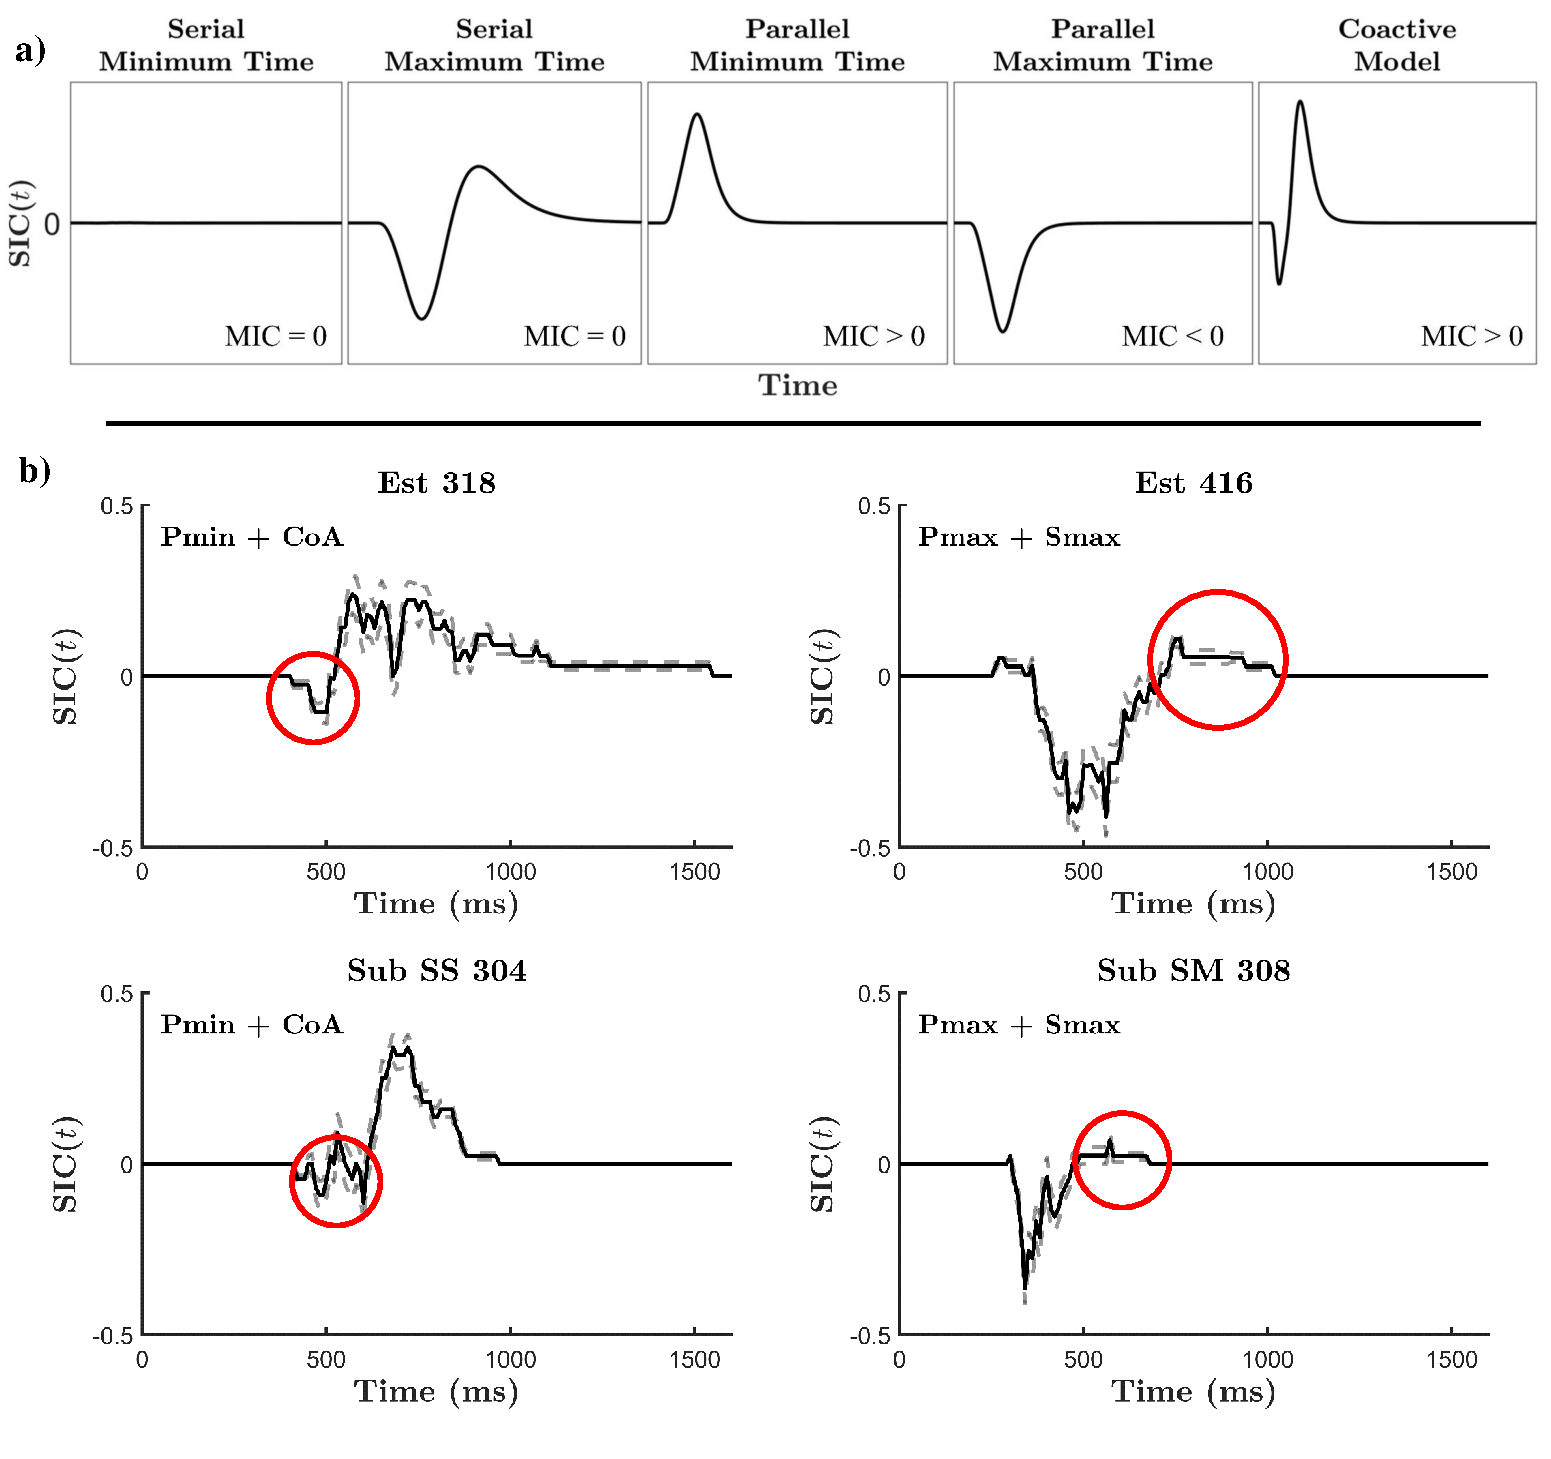
\includegraphics[width=\linewidth]{Figures/Subitizing/MixtureFigure.pdf}
\caption{a. The five canonical SIC functions. b. potential SIC model mixtures from the (top) estimation task, and (bottom) subitizing task. Left: parallel minimum-time models mixed with a coactive model. Right: parallel maximum-time models mixed with a serial exhaustive model. Identifying mixture signatures are circled in red.}
\label{fig:subSICmix}
\end{figure}

Participants Est 416 displays a negative SIC($t$) function, with a late positive deviation. The majority of the SIC($t$) function matches the predictions of a parallel maximum-time processing model; however, the late positive `blip' is indicative of a serial maximum-time model. This signature might suggest that, on a small proportion of trials, processing architecture switched from being parallel maximum-time to serial maximum-time. A similar mixture model is displayed by participant Sub SM 308. 

Visual identification of processing mixture models is rather subjective. Without the ability to identify mixture models through a non-parametric method (à la SFT), previous research has turned to parametric methods of mixture model classification \cite{Little2011, Moneer2016, Cheng2017}. In the following Chapter, we will address this limitation to the SFT machinery. First, we will systematically vary and combine the relative proportions of component processing models and express these mixtures visuallly with our distributional response-time measures. Then, we will extend the tools of SFT and consider a non-parametric method for identifying mixture models. 
\color{black}

\subsection{Conclusion}
Often in life, we need to subitize a set of items, be it coins in our wallet, people in a queue, or discs in a research laboratory\footnote{Admittedly, this is more common for some than others}. Little research has been conducted on how we subitize multiple item-sets, and no research has considered the cognitive architecture or workload capacity, experienced by this system. This is the first known study to address this question, and in so doing, apply the machinery of SFT to subitizing systems. Results of the current study align with findings from within the range of estimation. When asked to subitize two item-sets and decide if either contained less-than a criterion, participants experienced severe limitations to workload capacity. The ubiquity of this finding between participants, and across large and small item-sets, has led us to speculate this might be caused by perceptual context effects. Within the range of subitizing, processing architecture was predominantly serial, yet, select participants displayed patterns consistent with parallel processing architectures. It appears that, while cognitive workload is limited in every individual, processing architecture varies. 

%% AMI DONE 31/10/2019 @@@@@@@@@
 
\chapter{Mixture processing models} 

\label{Chapter 5}

\lhead{Chapter 5. \emph{Mixture models}}
\vspace{3cm}
\newpage

% New Sections for Ami to read
% - Sections highlighted in red in intro and discussion. 
% - I replaced the introductory proofs with a Figure to illustrate how channel RTs were combined to produce the canonical models (your suggestion from earlier this year, I think it works.)

%%AE: please make sure the figures are in good shape Paul, some ( 5.5, 5.6, 5.7, 5.8; perhaps others?) seems to be very low res, which makes them hard to see
%PG: Yep, this has now been fixed. Not sure what caused that.

\noindent
The results of this Chapter appear in the published manuscript `Systems factorial technology analysis of mixtures of processing architectures' \cite{Little2018mixmodel}.

\section{Chapter overview}
In a complex and ever changing environment, people must often process information from multiple sources. In previous Chapters, we have described how information processing systems may be diagnosed by several key attributes using SFT \cite{Townsend_1995, Townsend_2004, Little2017}. These attributes include the architecture (parallel vs serial), stopping-rule (exhaustive vs self-terminating), workload capacity (limited, unlimited, or super), and (in)dependence of the processing channels (facilitatory, independent, or inhibitory). SFT allows the identification of qualitatively different patterns of information processing models based on non-parametric analysis of response-time data. The purpose of this Chapter is to extend the application of SFT to those cases where there is a probabilistic mixture of two qualitatively different processing architectures. 

Humans display remarkable flexibility in how we combine and process information. For example, as we contemplate everyday situations, we can shift our attention to `low-level' perceptual or `high-level' conceptual aspects of a scene, (\eg a set of red items vs a vine of tomatoes), retrieve memories of an experience, (\eg numerical value `AND' guests for dinner tonight), and integrate these source to make a decision, (\eg I will need six of these tomatoes for dinner tonight). The integration of these different processes implies that, rarely, a processing system would purely reflect a singular set of attributes, (\eg entirely parallel or entirely serial). Mixtures of different processing models are likely to describe many everyday decisions, including categorization \cite{Little2011, Moneer2016, Cheng2017, Griffiths2017}, visual working memory \cite{Donkin2013}, controlled vs automatic processing \cite{Shiffrin1977,schneider1977controlled}, and comparative numerosity.

In the previous Chapter, we considered the possibility that response-times might reflect a mixture of two processing architectures. These mixtures may occur when different processing architectures are used on different trials of an experiment. For example, within numerical comparisons, a serial processing architecture may be adopted when quantities are near a criterion and workload is high, yet, when quantities are far from the criterion, processing architecture may switch to parallel. Similarly, mixtures of processing architecture may occur when channels move from being dependant, to independent, (\eg coactive to parallel). In the previous Chapter, we provided two example of such mixtures, however, examples also exist in other realms of cognition. For example, accessing memories might occur through the coactive pooling of information; yet, the decisional process may occur via independent-channels, in either parallel or serial.

Mixtures of processing architecture may describe many cognitive processes, yet, the signatures of these models have not been identified for the survivor interaction contrast and capacity coefficient. In this Chapter, we will generate and report SFT predictions for model mixtures, (\eg parallel vs serial), using the SIC($t$) and capacity coefficient. We will systematically vary the relative proportions of each component model, and visualize these mixtures with our distributional response-time measures. As the reader will soon see, results from these mixture models are different from those typically found using canonical or `pure' processing models and in some instances, reflect those mixtures reported in the discussion of Chapter \ref{Chapter 4}.

\section{Response-time mixtures}
The time taken to make a decision reflects a mixture of cognitive processes. For example, \citeA{luce1963detection} characterized a decision as the combination of external information and internal biases; whereas \citeA{Falmagne1965} characterised fast and slow responses as the mixture of preparatory and reactionary states, (\ie proactive and reactive control; \citeauthor{braver2007}, 2007). These accounts describe how cognitive processes mix, and the impact such mixtures have on decision response-times; yet, provide no insight into the mixture of processing systems --- how information channels mix and the effect this has on RT. 

Processing system mixture models have been of interest to the SFT community. In a recent special issue on SFT, \citeA{TillmanStopping} assessed how the SIC changed over mixtures of system stopping-rule (exhaustive vs self-terminating), within parallel and serial processing architectures. They observed smooth changes in canonical form, as relative mixture proportions shifted in favor of one processing model to another (Figures 1--2 of their paper). However, this investigation was limited to those instances where processing channels did not interact. Prior to this study, \citeA{eidels2011} investigated parallel models that allowed interactions across processing channels. Using both the SIC and capacity coefficient, \citeA{eidels2011} showed smooth changes in canonical form, from parallel facilitatory (coactive) channels, to parallel inhibitory channels (Figure 3 of their paper). 

The current Chapter will extend the work of both \citeA{TillmanStopping} and \citeA{eidels2011}. Here, we consider the impact of mixture models when processing architecture moves from parallel to serial, and when processing channels move from independent to facilitatory \cite<à la>{eidels2011}. As processing architecture and workload capacity are closely related, we will visualise these mixtures using both the SIC and capacity coefficient. Given the insights of \citeA{TillmanStopping}, the current work will be restricted to those cases where stopping-rule does not change.

Restricting our investigation to mixtures of processing architecture, and not mixtures of stopping-rule, makes sense under experimental settings. When a task requires the exhaustive processing of two information-sources, (\eg where channel A `AND' channel B must be a target), a self-terminating stopping-rule becomes a liability. Similarly, when a task requires only a single-target in either location, (\eg where channel A `OR' channel B must be a target), an exhaustive stopping-rule becomes non-strategic. In the SFT literature, we term these `AND' and `OR' tasks respectively. Importantly, these task-types are always tested independently, either in separate blocks or separate experiments. As such, from trial-to-trial, it is unlikely that stopping-rule would change when the task-requirements are always exhaustive, or always self-terminating. 

\section{AND vs OR capacity}
Assessing the system architecture and workload capacity of AND and OR tasks has been a key contribution of SFT. Measures of processing architecture --- the MIC and SIC --- are equally applicable regardless of task stopping-rule; the capacity coefficient is not. In a typical OR design, a participant should respond target present, (\ie YES), if any signal is present. By contrast, in a typical AND design, a target present response should only be given if both targets are present. Figure \ref{fig:Ch5_AndvsOR} illustrates correct responses in an `OR' and `AND' task, using stimuli from a classical dot-detection task \cite{Townsend_1995}. Here, responses are equivalent across tasks for double-target (AB) conditions, but differ between tasks for single-target conditions (A or B). The difference between redundant OR processing, and exhaustive AND processing, requires a unique formulation of the capacity coefficient for each task-design. 

\begin{figure}[htb]
\centering
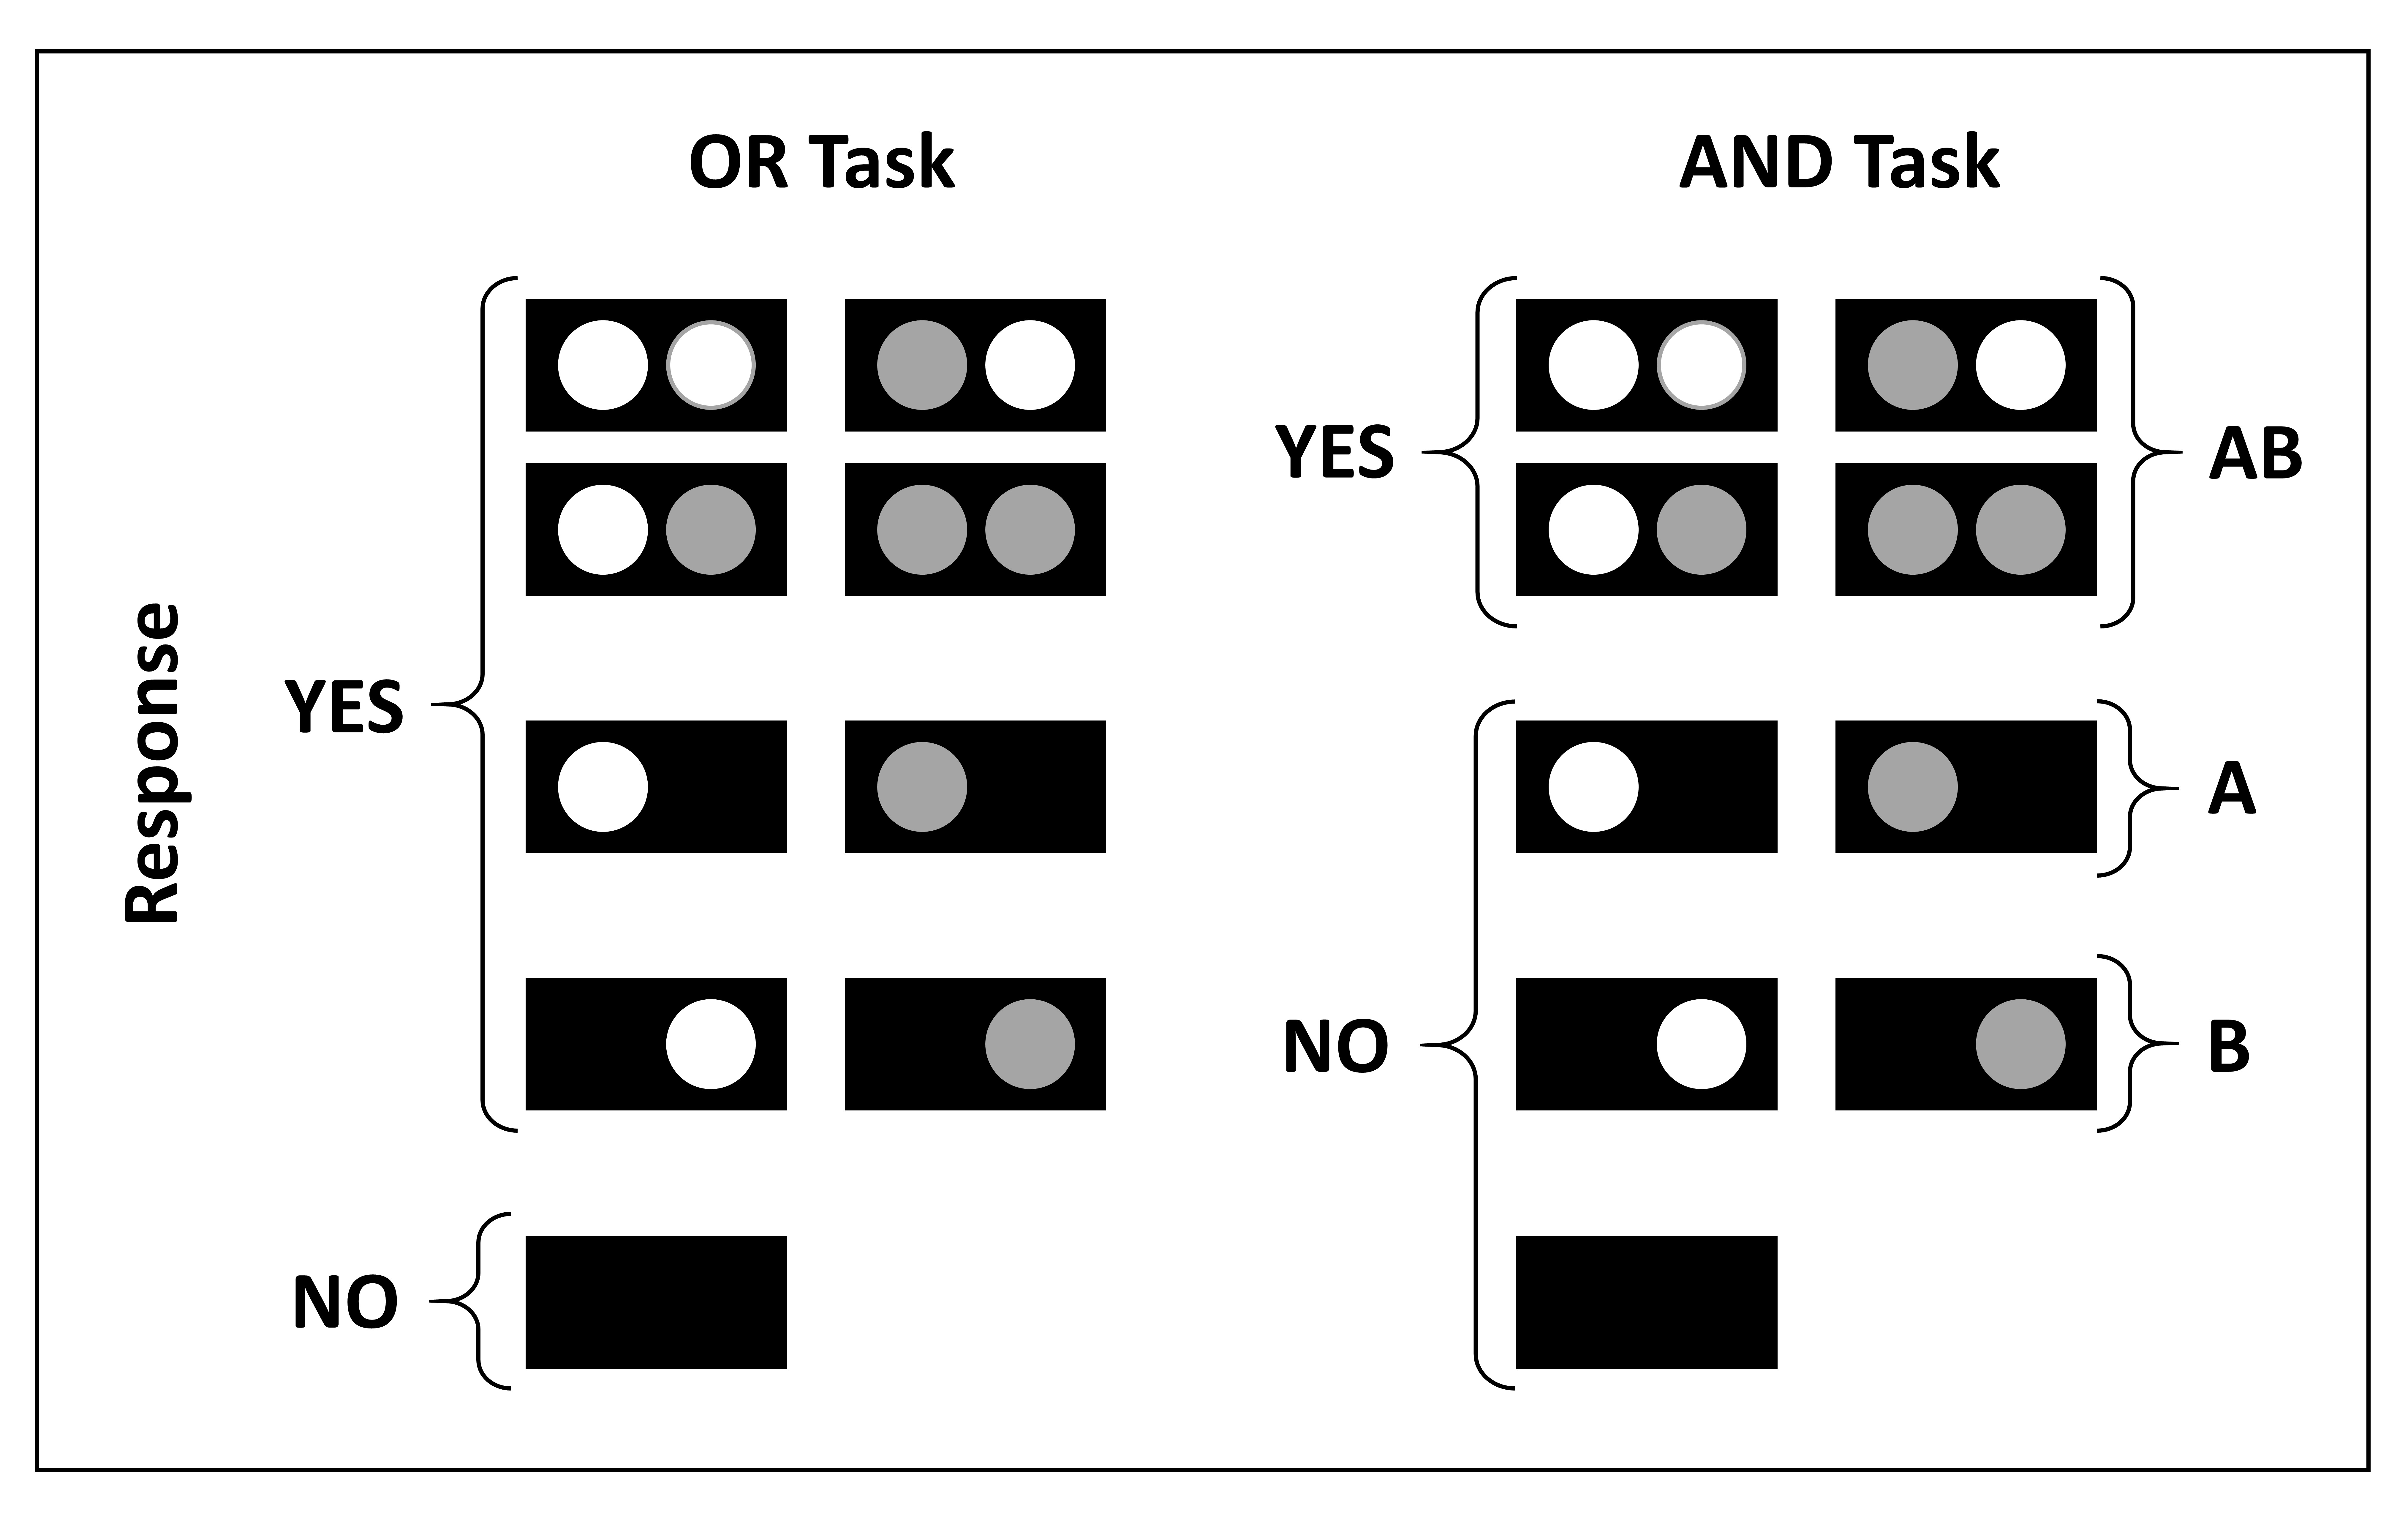
\includegraphics[scale=.6]{Figures/Mix/AndvsOR.jpg}
\caption{Stimuli from the classic redundant-target double-factorial paradigm of Townsend and Nozawa (1995), with responses mapped for an OR (left) and AND (right) task design. AB: double-target. A: single-target left. B: single-target right.}
\label{fig:Ch5_AndvsOR}
\end{figure}

\subsection{OR capacity}
In Chapter 1, we covered the capacity coefficient for an OR task. In an OR task, capacity is measured relative to the self-terminating (minimum-time) benchmark of unlimited capacity, independent-channel, parallel (UCIP) race-model. Under this model, double-target processing times are equal to the sum processing times of each target-channel in isolation. These processing times can be expressed in terms of their distribution over time using a survivor function. A survivor function [S($t$)] characterizes the probability of a process not-continuing by time $t$; it is calculated as one minus the cumulative distribution function [1 - F($t$)]. This can also be represented in terms of a cumulative hazard function [H($t$) = -$\log$ S($t$)]. Under the self-terminating UCIP model, the capacity coefficient compares double-target finishing times [H$_{AB}$($t$)] to the finishing times of each channel in isolation [H$_{A}$($t$), H$_{B}$($t$)] and may be expressed as:

\begin{equation}
	\rm C_{OR}(\t) = \frac{-\log[S_{AB}(\t)]}{-\log[S_{A}(\t)] - \log[S_{B}(\t)]}
    \label{eq:Cor}
\end{equation}

\subsection{AND capacity}
For an AND task, capacity is computed compared to the maximum time benchmark of the UCIP exhaustive model, (\ie the slowest processing channel times). This can be specified in terms of the reverse integrated hazard function, [\ie the logarithmic transformation of the cumulative distribution function, -$\log$F($t$)], for double-target processing channels, compared to the reverse integrated hazard function predicated by the maximum of each single-target processing channel. The AND capacity coefficient can be expressed as: 

\begin{equation}
    \rm C_{AND}(\t) = \frac{-\log[F_{A}(\t)]-\log[F_{B}(\t)]}{-\log[F_{AB}(\t)]}
    \label{eq:Cand}
\end{equation}

As the \Cor and \Cand are both calculated under the assumptions of a UCIP model, each under their respective self-terminating or exhaustive stopping-rules; interpretations remain the same between each function. An unlimited capacity system that is unaffected by additional processing channels, predicts C($t$) = 1. A limited capacity system that slows with additional processing channels, (\ie slower double-target trials), predicts C($t$) $<$ 1, and a super capacity system that speeds with additional processing channels, (\ie a coactive model), predicts C($t$) $>$ 1.

\section{Pure to mixture models}
Over the course of this thesis, much time has been dedicated to the assessment of system architecture using the SIC. As illustrated in Chapter 1, each combination of stopping-rule and processing architecture, predicts a qualitatively unique SIC($t$) function (see Figure \ref{fig:SIC}). Identifying these `pure' processing models in empirical data has been the primary aim of SFT, with many statistical tools being developed to aid this identification \cite{houpt2010statSIC, houpt2012statCap, houpt2017hierarchical, houpt2017bayesSIC, Houpt2016, Thiele2017}. While some efforts have been made to identify mixture models in empirical data \cite<see>{Little2011, Moneer2016, Cheng2018}, the canonical signatures of the SIC($t$) and C($t$) have not been established for these mixture processes. 

In the following section, we will systematically simulate the range of potential models for various combinations of processing architecture within both `OR' and `AND' task designs. We will then visualise these mixture models using the distributional response-time measures, the SIC($t$) and C($t$). We aim to provide a new set of canonical SIC($t$) and C($t$) predictions, with which mixture models can be identified.

\section{Simulations}
To simulate mixtures of processing architecture and capacity, started by simulating the five `canonical' system models: parallel self-terminating, serial self-terminating, parallel exhaustive, serial exhaustive and coactive. 

\color{\Red}
\subsection{Canonical models}
We simulated each of the independent processing channels of the serial and parallel models as well as a coactive models (where input from two channels is combined prior to decision) using pairs of Poisson accumulators, Linear Ballistic accumulators \cite<LBA;>{Brown2008} and random walk accumulators. Although theoretically different, these accumulators have two similar components: a rate parameter and a decision threshold parameter. The rate parameter dictates the rate evidence accumulates towards the decision threshold which, once crossed, terminates the accumulation process and yields a channel completion-time. %AE: discard >>> \footnote{The Poissson accumulator is a distribution of RTs rather than a sequential accumulation process, however, the basic principles needed to grasp channel RT in each processing model remains unchanged.}. 
Manipulation of the rate parameter simulates high and low salience conditions, given a fixed decision threshold. Finally, channel completion-times from each of the two accumulators are combined using the specific operational order and decision rules dictated by the generating system model.

% AE: for each channel separately i suggest to use completion time  (or processing) time -- but NOT response time, as individual channel do not emit a response
% PG: Yep, fixed. Thanks

Figure \ref{fig:Ch5_ProArch} illustrates the operational order and decision rules by which channels were combined and response-times (i.e., channel completion times) were simulated for double-target trials under each canonical processing model. Note that for coactive processing models we assumed complete cross-talk between the channels such that the coactive accumulator rate was equal to the summed rate of both single target accumulators \cite<see>{Johnson2010b}. Simulating single-target and double-target trials under these five canonical models, allows us to generate simulated SIC(\textit{t}) and C(\textit{t}) functions. 

\begin{figure}[htb]
\centering
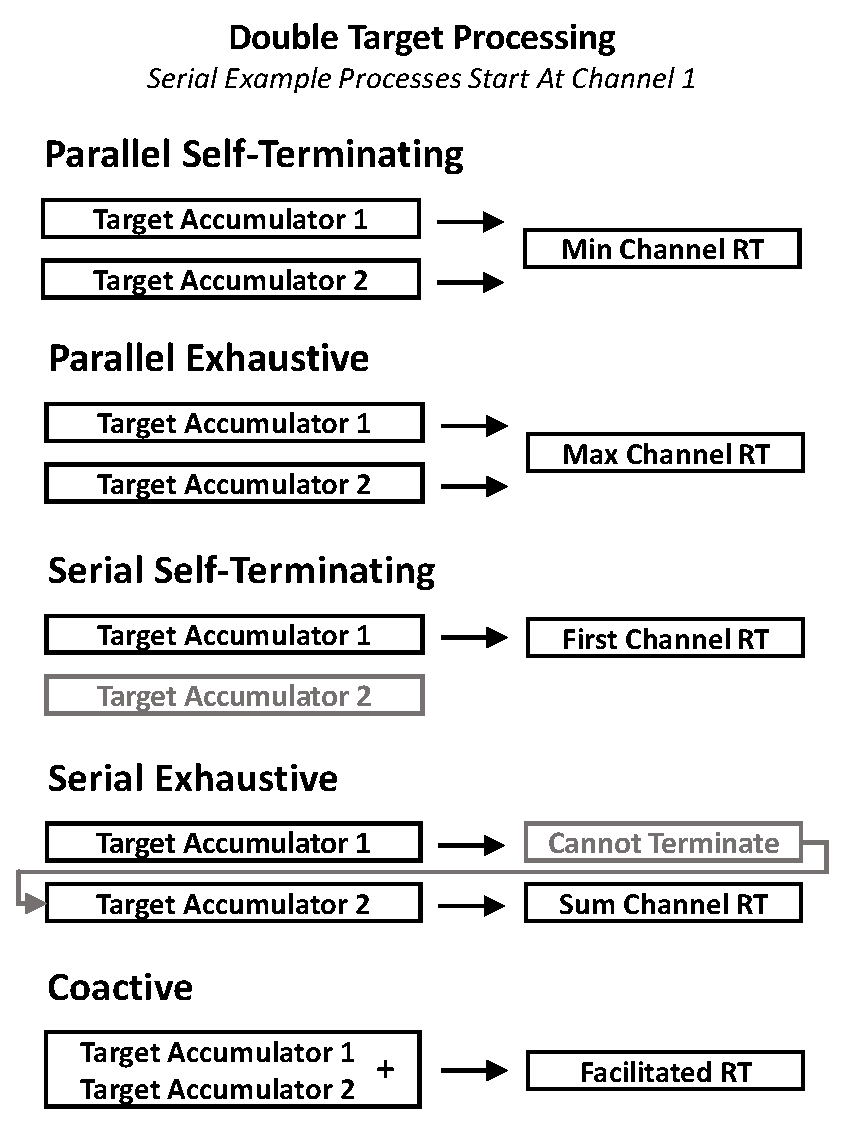
\includegraphics[scale = .85]{Figures/Mix/DoubleTargetProcessing.pdf}
\caption{Illustration of double-target channel operations used to simulate the five canonical processing models: parallel self-terminating, parallel exhaustive, serial self-terminating, serial exhaustive and coactive. Accumulators were either pairs of Poisson, linear ballistic or random walk accumulators. Single target channel RTs were simulated by their respective single accumulator.}
\label{fig:Ch5_ProArch}
\end{figure}

\color{black}

\subsection{Mixture models}
Mixture models were computed as the additive mixtures of the component canonical models, with $p$ the probability that the mixture model used a parallel process, and $1-p$ the probability that the mixture used another process (coactive or serial). While our modeling allowed for mixtures of architectures (serial, parallel, and coactive), it did \emph{not} allow for a mixtures across stopping-rules. For the OR decision rule, we used the parallel self-terminating model and the serial self-terminating model, and for the AND decision rule, we used the parallel exhaustive and serial exhaustive models. The stopping rule distinction does not apply to the coactive processing model.

Mixture models represent cases where across different trials the observer probabilistically adopts a different processing model. We simulated the predictions of the mixture models for the capacity coefficient and SIC with the probability of parallel processing, $p$, set to $0, .2, .4, .6, .8,$ or $1$. For all of the simulations, we used parameter values for which each channel produced distributions which had roughly the same mean RT, constraining the various canonical models to roughly the same time range. This constraint is driven by empirical observations.

When the means of the distributions diverge by a large extent, the functional predictions of each component SIC can become separated in time. For example, a negative parallel SIC might be followed by a serial SIC that produces a second negative component and then a positive component. Such a strong separation in the empirical data is yet to be witnessed \cite<\eg>{Little2011, Moneer2016}. We suspect this is because mixtures are unlikely when one component process is much less efficient than the other. As such, our simulated mixture models will focus exclusively on those instances where both mixture processing models are roughly equivalent in processing efficiency. 

\subsection{Poisson accumulator}
We simulated the completion times of each processing channel by a number of accumulated counts distributed as a Poisson random variable with a rate parameter $\lambda$ and a decision threshold parameter $a$. We use the subscripts 1 and 2 to indicate which of the two channel components of the model we are referring to. For all models, we set $a_1 = a_2 = 10$. For the capacity simulations, we set $\lambda_1 = \lambda_2 = .05$. For the SIC simulations, we set $\lambda_L = .02$ and $\lambda_H = .05$. Simulated processing-times were sampled from the relevant parallel model at a probability of $p$, and from the alternate model with a probability $1-p$. 

A benefit of the Poisson accumulator is that this analytic model is easily subjected to formal mathematical proofs. A formal mathematical description of the Possion accumulator for each processing channel is provided in the supplementary materials S3 (equations \ref{eq:poisspdf}--3). Formal proofs for each canonical processing model (equations \ref{eq:parst}--\ref{eq:serex}), each mixture model (equation \ref{eq:mixtures}), the capacity coefficient mixture process (equations \ref{eq:Fmix}--\ref{eq:CtMix}), and the SIC mixture process (equation \ref{eq:SICmix}) are all provided in supplementary materials S3. These proofs were used in the production of the following Poisson mixtures and are a formal expression of the processes illustrated in Figure \ref{fig:Ch5_ProArch}. For the purpose of exposition, these proofs will not be focused upon further and our simulated results will now be presented.

\subsubsection{Capacity predictions} 
The capacity predictions for two kinds of mixture models, parallel processing coupled with either serial or coactive processes, for both the OR and AND case, are shown in Figure~\ref{fig:Ch5_CapPoisson}. For the coactive/parallel mixture model, as $p$ increases from 0 to 1, the predictions clearly reflect a smooth transition from the unlimited capacity parallel model predictions to the supercapacity coactive model predictions. Conversely, for the parallel/serial mixture model, the capacity predictions move smoothly from unlimited to limited capacity. 

For both the OR and the AND capacity functions, the presence of any amount of coactivity causes changes in the limit behavior of the function. For \Cor the left limit increases sharply reflecting the increased rate of processing for the double target as smaller values of $t$ relative to the single targets. For the single targets, there is no difference between a coactive or a parallel process since there is by definition only a single source of information. Likewise, for the AND capacity there is an increase in the \Cand function for smaller values of $t$. The opposite effect arises for the mixture of serial and parallel processing. Again, for the single targets, there is no difference between the serial and parallel predictions, but introducing any proportion of serial processing into the mixture leads to a decrease in capacity at longer values of $t$. Note that when the process is completely serial, \Cor = .5 for all $t$ indicating limited, fixed capacity. 
 
\begin{figure}[htb]
\centering
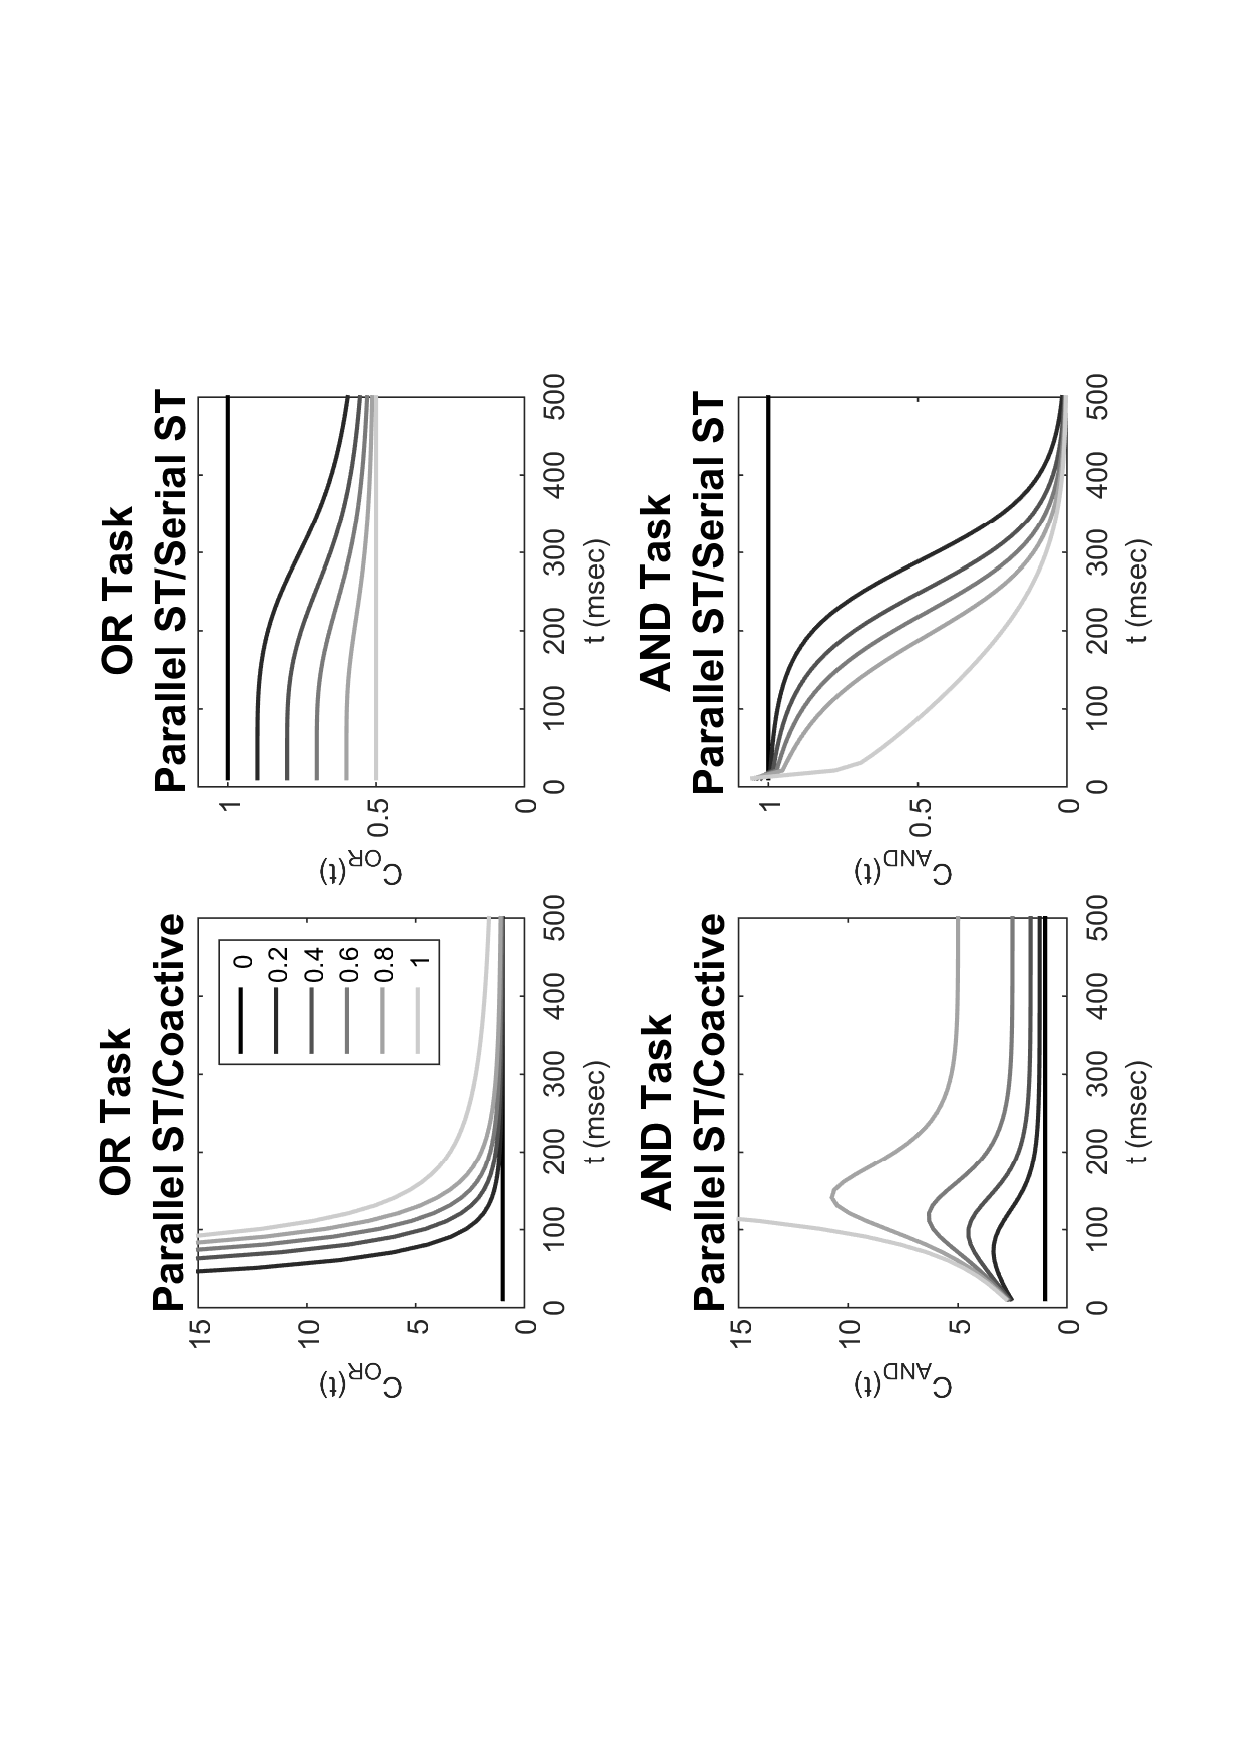
\includegraphics[scale=.7, angle=-90]{Figures/Mix/Figure_2.pdf}
\caption{Top: OR capacity coefficient predictions for the coactive/parallel self-terminating (left) and serial/parallel self-terminating (right) mixture models. Bottom: AND capacity coefficient predictions for the parallel exhaustive/coactive (left) and parallel exhaustive/serial exhaustive (right) mixture models. Simulations of each component process were instantiated as a pair of Poisson accumulators.}
\label{fig:Ch5_CapPoisson}
\end{figure}


\subsubsection{SIC predictions} 
The SIC predictions for the mixture models are shown in Figure~\ref{fig:Ch5_SICpoisson}. Like the capacity predictions, both sets of predictions transition smoothly between the parallel predictions and coactive or serial predictions for the parallel/coactive and parallel/serial models, respectively. 

\begin{figure}[htb]
\centering
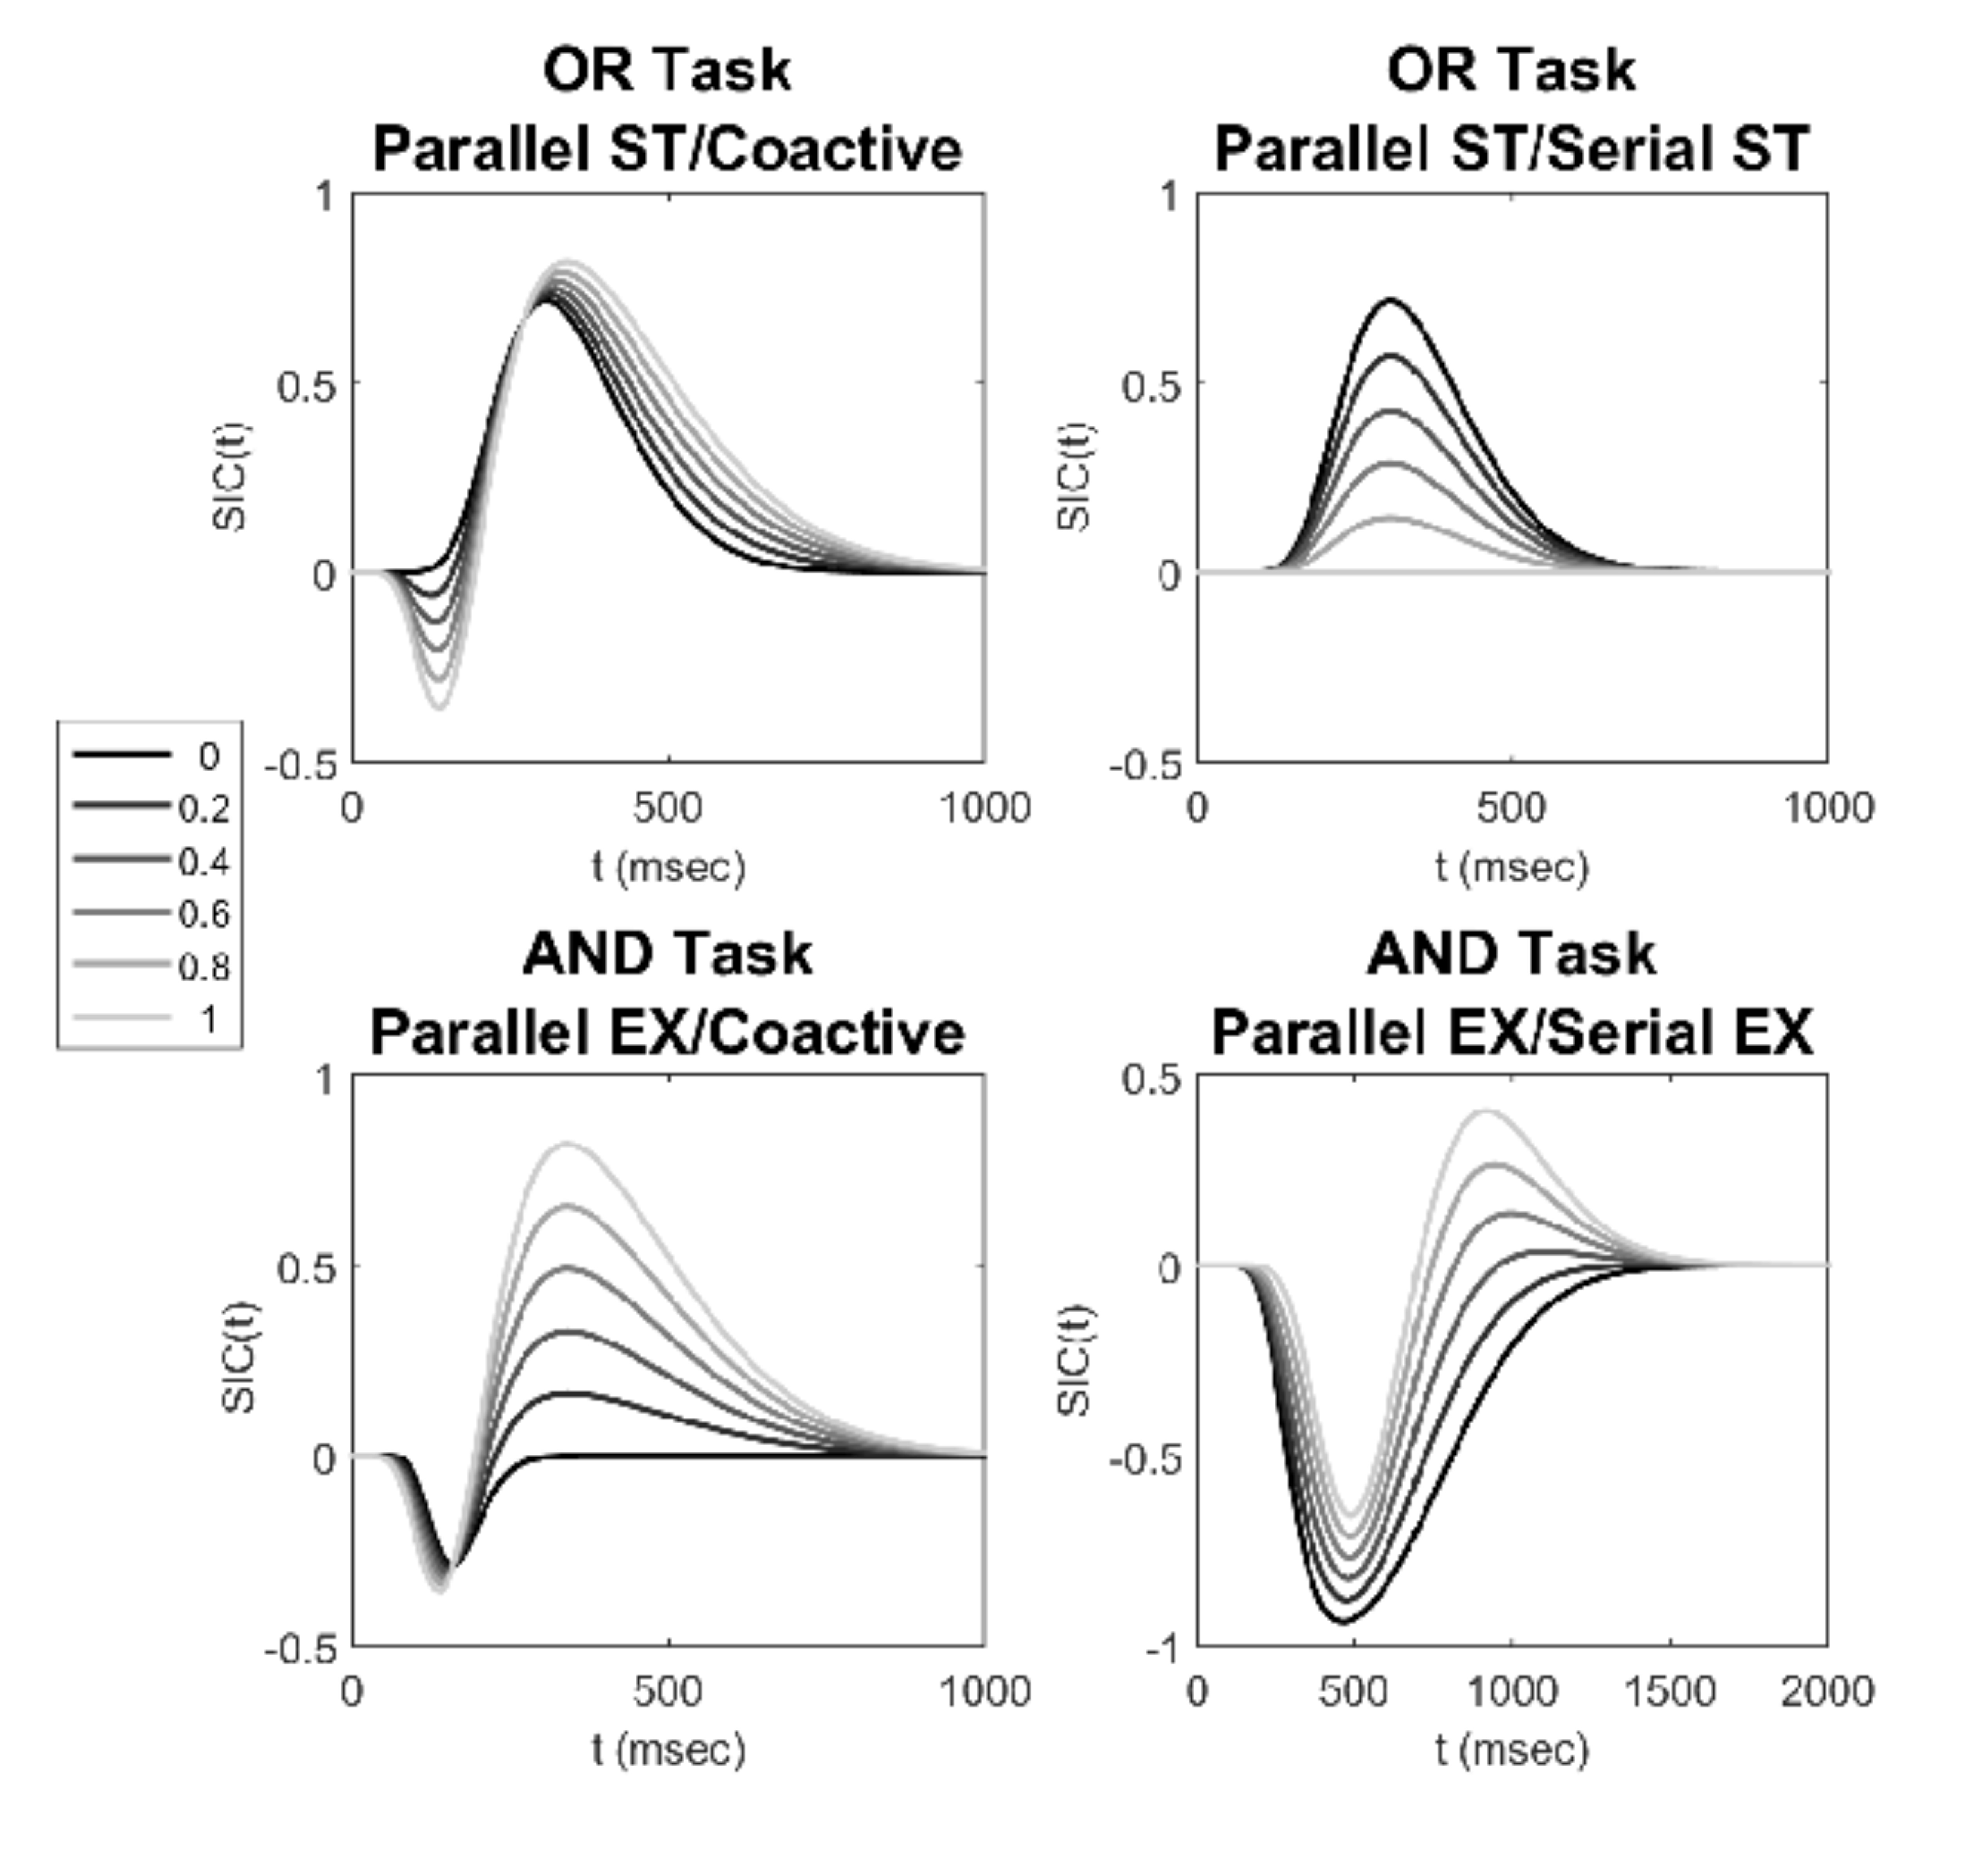
\includegraphics[scale=1]{Figures/Mix/SICpoisson.jpg}
\caption{Top: survivor interaction contrast (SIC) predictions for the self-terminating coactive/parallel (left) and self-terminating serial/parallel (right) mixture models. Bottom: survivor interaction contrast (SIC) predictions for the exhaustive coactive/parallel (left) and exhaustive serial/parallel (right) mixture models. Simulations of each component process were instantiated as a pair of Poisson accumulators.}
\label{fig:Ch5_SICpoisson}
\end{figure}


\subsection{Interim summary}
Mixing serial, parallel, and coactive processes results in a wide range of SFT signatures that go well beyond the canonical signatures initially studied by \citeA{Townsend_1995}. Relaxing the assumption that responses on all trials in an experiment are homogeneous (though stochastic) and come from a single process by combining processes from different distributions with different mixture-probabilities, allows a fair amount of flexibility in the predicted signature. This flexibility is also reflected in the simulated behavioral outcomes, as measured by \SIC and \Ct which change with the mixing proportion $p$. Thus, instead of a unique and well-defined SIC signature for a parallel model (say, positive for all time $t$), a mixture of parallel and coactive processes could predict anything between an all-positive SIC to a partly-negative SIC (for early $t$) to a partly-positive SIC (for longer $t$), as shown in the top left panel of Figure~\ref{fig:Ch5_SICpoisson}. 

Importantly, our mixture model simulations reveal that changes to the \SIC and C(\textit{t}) are completely \textit{predictable} (as suggested informally by \citeNP{Fific2008}, and later by \citeNP{TillmanStopping}). That is, the \SIC and \Ct signatures of probability mixtures are bounded between the extreme signatures defined by $p$=0 and $p$=1. Moreover, within these bounds they change in a predictable and systematic way, looking similar to parallel signature for small $p$, and gradually taking the form of the alternate component in the mixture as $p$ increases. To further validate our findings, we extended the scope of our simulations, and simulated these mixture models with different underlying processes.

\subsection{Computation simulations: LBA}
We simulated the mixture model results under the assumption that each channel was an independent linear ballistic accumulator, with an error drift rate set to zero. Each of the accumulator processes is characterized by the following parameters: drift rate $\nu_i$, for each of the simulated channels $i$, a response threshold, $b$, the width of the uniform starting point distribution, $A$, and the standard deviation of the normal drift distribution representing between trial variability, $s$. Response thresholds were set to 3, starting point variability was set to 2 and the standard deviation of the drift was set to 1. The non-decision time parameter, $Ter$, was set to 0. Drift rates for each model for the SIC and capacity coefficient simulations are shown in Table \ref{tab:lba_drifts}. 

\begin{table}[htb]
\centering
\caption{Drift rates for each stimulus component and their combination (Coactive) or individual stimulus component (Serial \& Parallel) for SIC and capacity coefficient mixtures. We use the A \& B values to simulate SIC($t$)$_{OR}$ functions, and X \& Y values to simulate SIC($t$)$_{AND}$ functions. Subscripts $h$ and $l$ refer to the salience of each channel. Coactive drift rates were identical for both OR and AND functions.}
\begin{tabular}{l l l l r r } 
\hline
Stimulus & Coactive   		& ~ & Stimulus   &  Serial 	& Parallel 	\\
\hline
$A_hB_h$ & 10.8             & ~ & $A_h$      & 7         & 7         \\
$A_hB_l$ & 6.8              & ~ & $A_l$      & 3         & 3         \\
$A_lB_h$ & 6.8              & ~ & $B_h$      & 7         & 7         \\
$A_lB_l$ & 2.8              & ~ & $B_l$      & 3         & 3         \\
$X_hY_h$ & 10.8             & ~ & $X_h$      & 7         & 7         \\
$X_hY_l$ & 6.8              & ~ & $X_l$      & 3         & 3         \\
$X_lY_h$ & 6.8              & ~ & $Y_h$      & 7         & 7         \\
$X_lY_l$ & 2.8              & ~ & $Y_l$      & 3         & 3    
\\
\hline
\hline
\label{tab:lba_drifts}
\end{tabular} 
\end{table}

To simulate the coactive LBA model, complete cross-talk between the processing channels was assumed, such that sharing the probability of a single count was always 1. Predictions for the coactive model were simulated by summing the drift rates sampled from two independent channels, $\nu_{1}$ and $\nu_{2}$. The drift rate for each independent channel was sampled from a normal distribution, centered on $\nu_i$, with standard deviation $s$. For each stimulus, 1 million RTs were simulated; RT predictions were binned by 5 msec ranging from 0 to 2,000 msec.

For the remaining models, individual channels were combined using equations quantitatively identical to the analytic proofs located in supplementary material S3, Equations~\ref{eq:parst}-\ref{eq:serex}. The results of these simulations are shown in Figures \ref{fig:capLBAmixture} and \ref{fig:sicLBAmixture}. To generate comparable mean RTs, the threshold and starting point parameters were decreased to 1.75 and 1.3 respectively, for parallel exhaustive models in the comparison of coactive and parallel exhaustive mixtures, and for serial exhaustive models in the comparison of serial and parallel exhaustive mixtures.

\begin{figure}[htb]
\centering
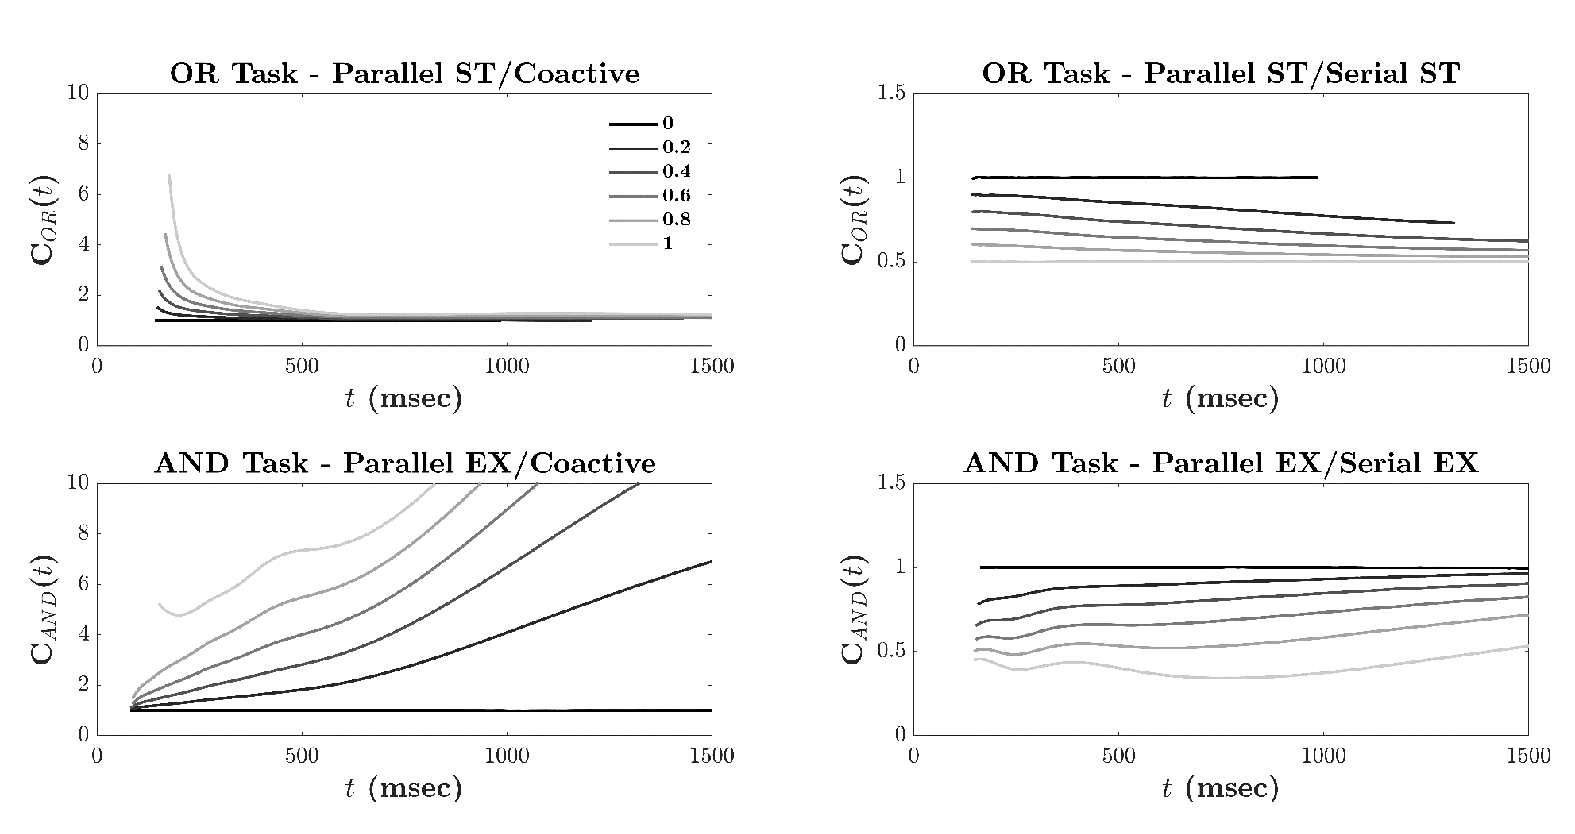
\includegraphics[scale=.6]{Figures/Mix/Figure_B1v3.pdf}
\caption{Linear ballistic accumulator predictions. Top: OR capacity coefficient predictions for the coactive/parallel (left) and serial/parallel (right) mixture models. Bottom: AND capacity coefficient predictions for the parallel/coactive (left) and parallel/serial (right) mixture models.}
\label{fig:capLBAmixture}
\end{figure}

\begin{figure}[htb]
\centering
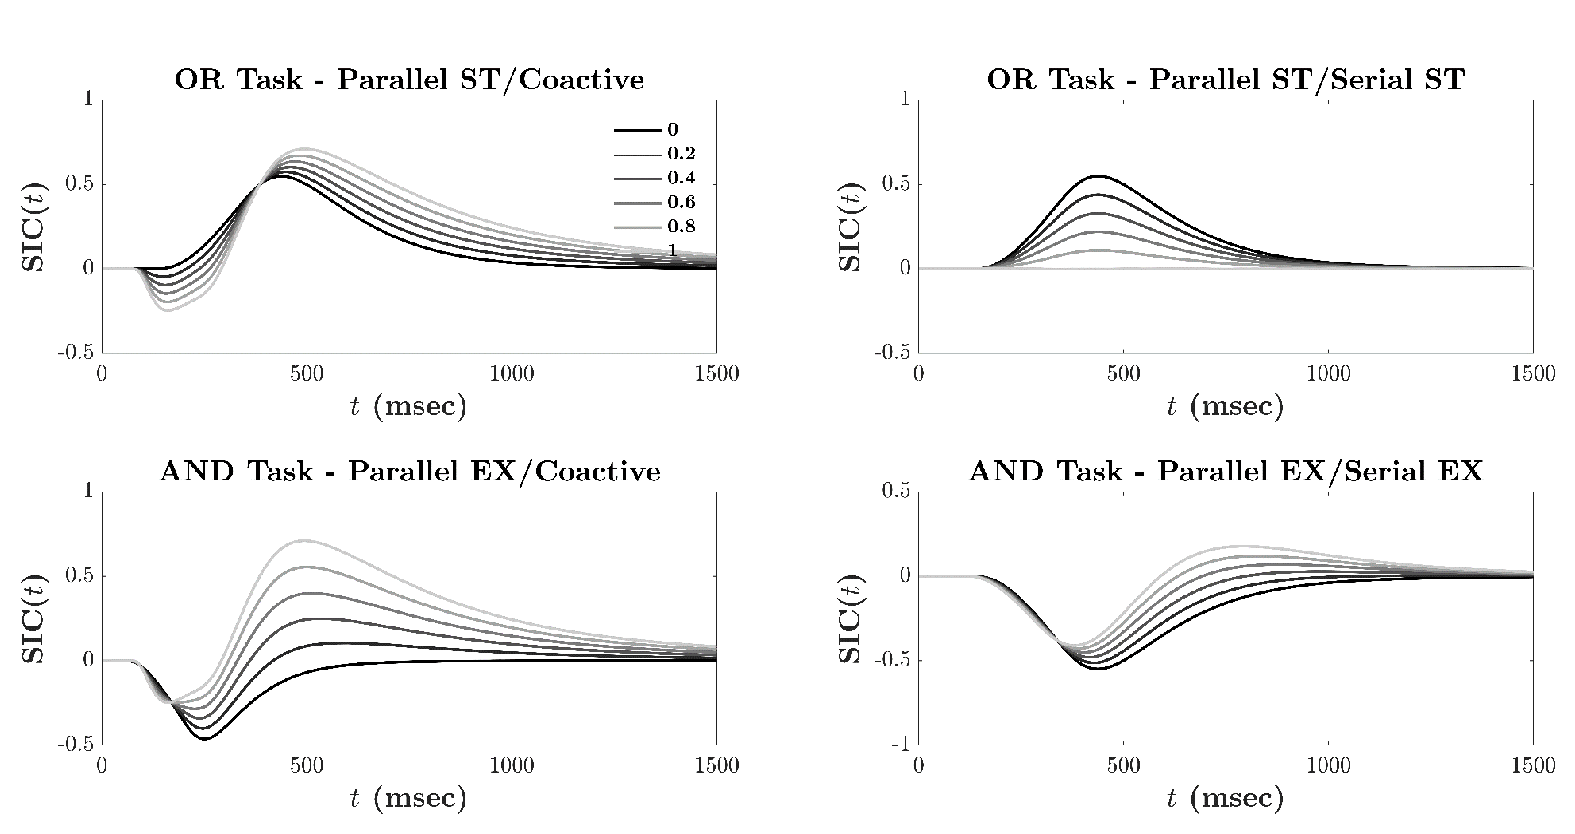
\includegraphics[scale=.6]{Figures/Mix/Figure_B2.pdf}
\caption{Linear ballistic accumulator predictions. Top: survivor interaction contrast (SIC) predictions for the self-terminating coactive/parallel (left) and self-terminating serial/parallel (right) mixture models. Bottom: survivor interaction contrast (SIC) predictions for the exhaustive coactive/parallel (left) and exhaustive serial/parallel (right) mixture models.}
\label{fig:sicLBAmixture}
\end{figure}


\subsection{Computation simulations: random walk}
We simulated the mixture model results under the assumption that each channel was a random walk. Each random walk is characterized by the following parameters: step rate $\nu_i$, where $\nu$ represents the rate at which discrete steps are sampled for each of the simulated channels $i$, threshold $a$ and bias $\beta$. Bias was kept constant at 0 for all simulations and target channel and error thresholds was set to 115 and -115, respectively.

Each step of the random walk was a discrete value of 1 or -1, with steps accumulating towards the upper or lower response threshold. Step rate $\nu$ of the random walk was a probability bound between 0 $\leq \nu \leq$ 1, with $\nu$ less than 0.5 increasing the rate at which negative steps were sampled, and $\nu$ greater than 0.5 increasing the rate at which positive steps were sampled. The non-decision time parameter, $T$er was set to 0. We adopted this assumption since we are primarily interested in mixtures of the decision stage of processing; however, it must be acknowledged that manipulations of salience may also affect non-decision processes like encoding. Step probabilities for each model in the SIC and capacity coefficient simulations are shown in Table~\ref{tab:RW_drifts}. 

\begin{table}[tbh]
\centering
\caption{Random walk step probabilities, reported in terms of $\nu$, for each stimulus component and their combination (Coactive) or individual stimulus component (Serial \& Parallel) for SIC and capacity coefficient mixtures. We use the A \& B values to simulate the SIC($t$)$_{OR}$ function and the X \& Y values to simulate the SIC($t$)$_{AND}$ function. The subscripts $h$ and $l$ refer to the salience of the channel.}
\begin{tabular}{l l c l c c } 
\hline
Stimulus & Coactive   	   & ~ & Stimulus   &  Serial 	  & Parallel 	\\
\hline
$A_h$ &     .64            & ~ & $A_h$      & .685        & .685        \\
$A_l$ &     .57            & ~ & $A_l$      & .63         & .63         \\
$B_h$ &     .64            & ~ & $B_h$      & .685        & .685        \\
$B_l$ &     .57            & ~ & $B_l$      & .63         & .63         \\
$X_h$ &     .64            & ~ & $X_h$      & .685        & .685        \\
$X_l$ &     .57            & ~ & $X_l$      & .63         & .63         \\
$Y_h$ &     .64            & ~ & $Y_h$      & .685        & .685        \\
$Y_l$ &     .57            & ~ & $Y_l$      & .63         & .63         \\
$A_hB_h$ &  $A_h$ + $B_h$  & ~ &   ~        & ~           & ~           \\
$A_hB_l$ &  $A_h$ + $B_l$  & ~ &   ~        & ~           & ~           \\
$A_lB_h$ &  $A_l$ + $B_h$  & ~ &   ~        & ~           & ~           \\
$A_lB_l$ &  $A_l$ + $B_l$  & ~ &   ~        & ~           & ~           \\
$X_hY_h$ &  $X_h$ + $Y_h$  & ~ &   ~        & ~           & ~           \\
$X_hY_l$ &  $X_h$ + $Y_l$  & ~ &   ~        & ~           & ~           \\
$X_lY_h$ &  $X_l$ + $Y_h$  & ~ &   ~        & ~           & ~           \\
$X_lY_l$ &  $X_l$ + $Y_l$  & ~ &   ~        & ~           & ~           \\
\hline
\hline
\label{tab:RW_drifts}
\end{tabular} 
\end{table}

\subsubsection {Coactive random walk model} To simulate the coactive random walk model, complete cross-talk between processing channels was assumed. Predictions for the coactive model were simulated by summing the the two independent accumulator channels, $\nu_{1k}$ and $\nu_{2k}$, at each step of the independent random walks, $k$. This is shown in Table~\ref{tab:RW_drifts} by the summation of the terms. For each stimulus, 100,000 RTs were simulated; RT predictions were binned by 5 msec ranging from 0 to 2,000 msec.

For the remaining models, individual channels were combined using the same procedures as the LBA and Poisson models. The results of these simulations are shown in Figures \ref{fig:capRWmixture} and \ref{fig:sicRWmixture}. To generate comparable mean RTs, the threshold parameter was decreased to 67 for parallel exhaustive models in the comparison of coactive and parallel exhaustive mixtures; and for serial exhaustive models in the comparison of serial exhaustive and parallel exhaustive mixtures.

\begin{figure}
\centering
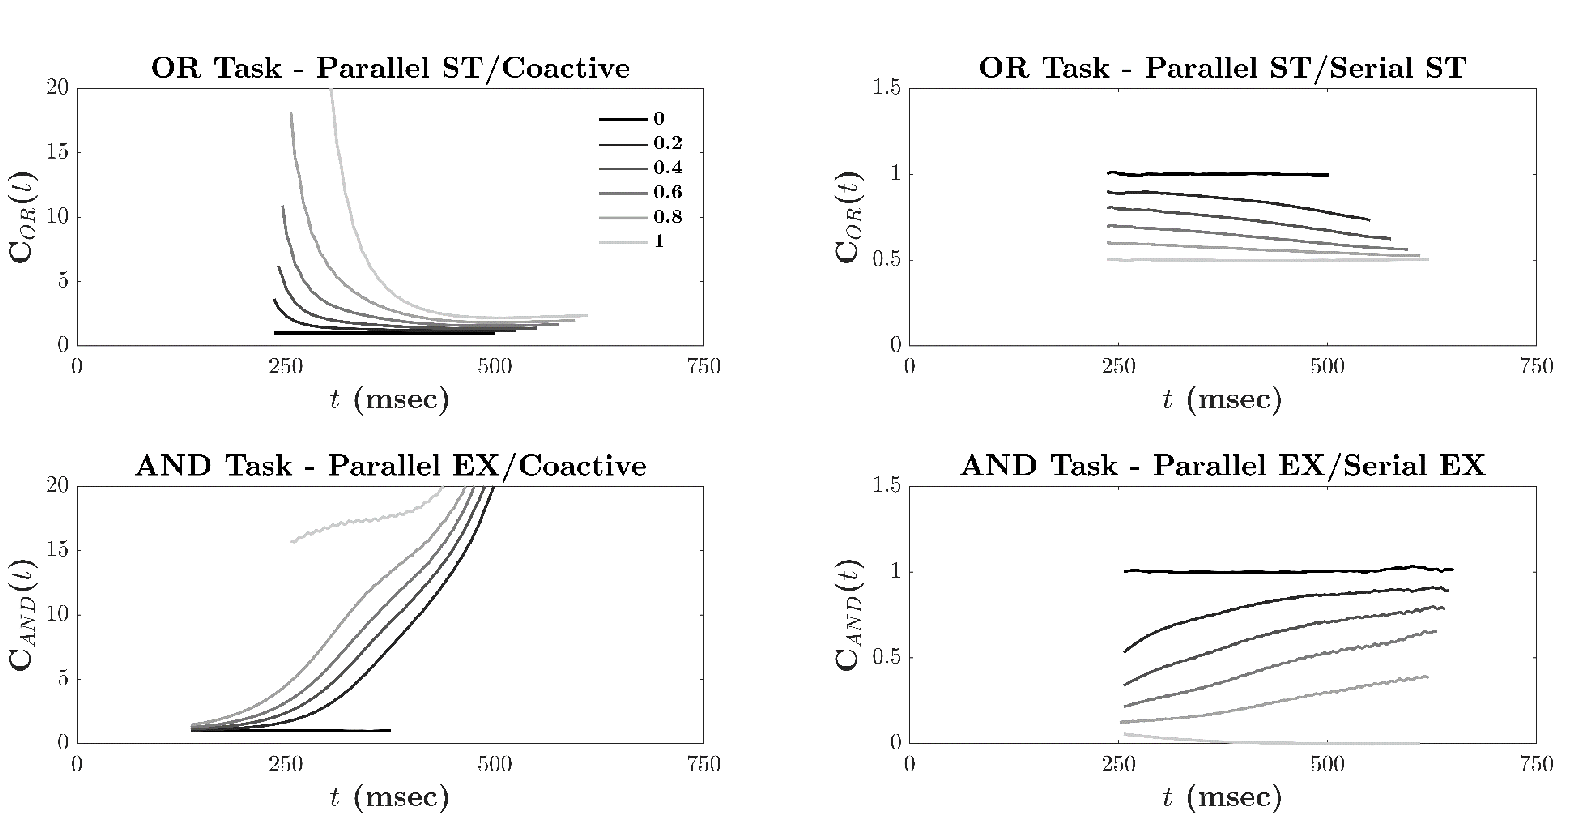
\includegraphics[scale=.6]{Figures/Mix/Figure_C1.pdf}
\caption{Random walk accumulator predictions. Top: OR capacity coefficient predictions for the coactive/parallel (left) and serial/parallel (right) mixture models. Bottom: AND capacity coefficient predictions for the parallel/coactive (left) and parallel/serial (right) mixture models.}
\label{fig:capRWmixture}
\end{figure}

\begin{figure}
\centering
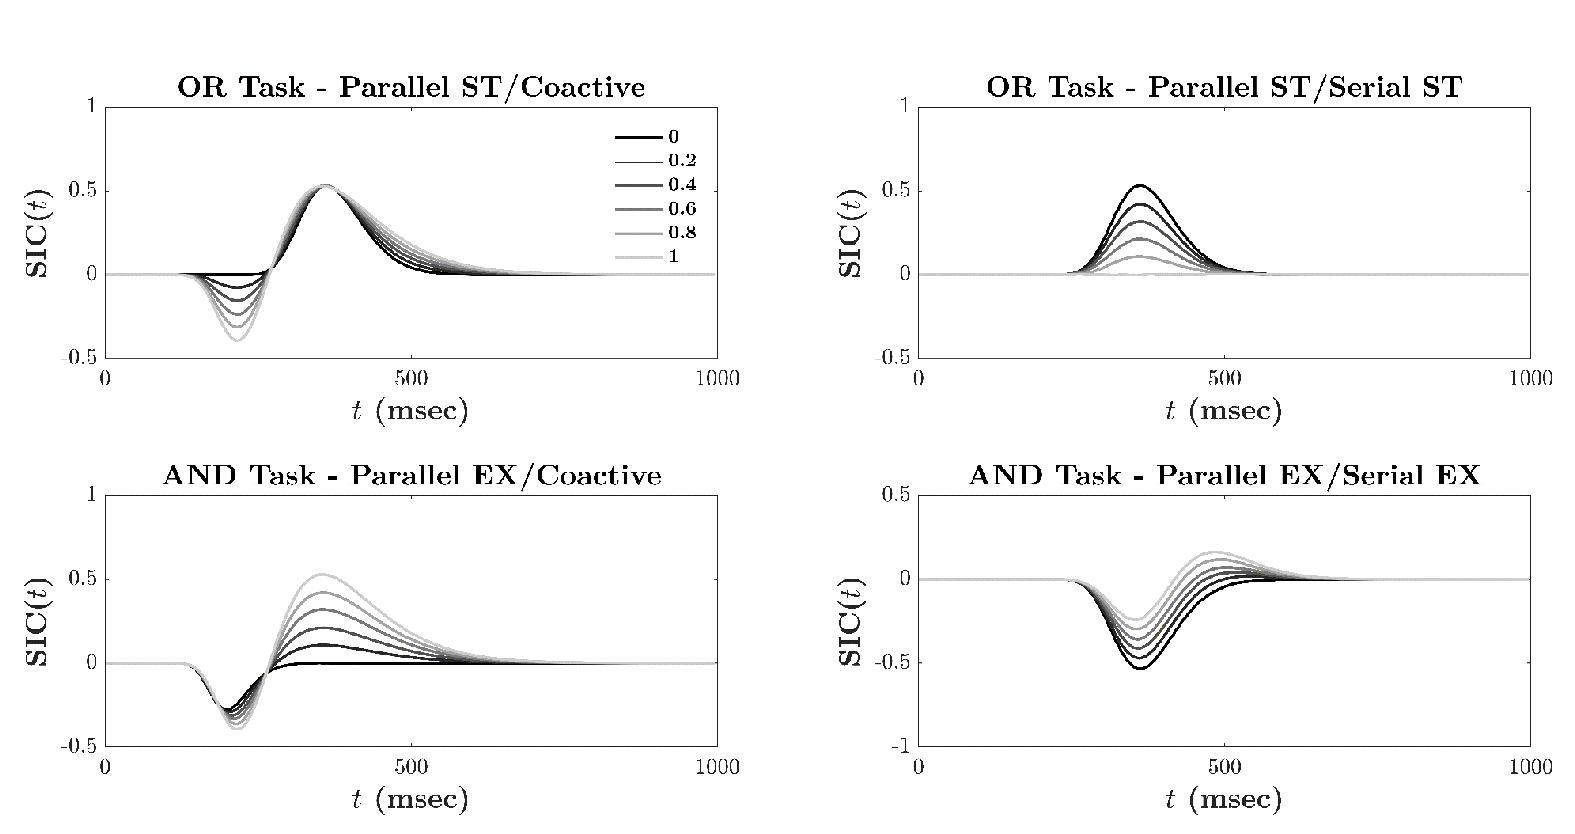
\includegraphics[scale=.6]{Figures/Mix/Figure_C2.pdf}
\caption{Random walk accumulator predictions. Top: survivor interaction contrast (SIC) predictions for the self-terminating coactive/parallel (left) and self-terminating serial/parallel (right) mixture models. Bottom: survivor interaction contrast (SIC) predictions for the exhaustive coactive/parallel (left) and exhaustive serial/parallel (right) mixture models.}
\label{fig:sicRWmixture}
\end{figure}


\section{Discussion}
% General Findings
The current investigation systematically varied the relative proportions of component `pure' system models, and visualized the SIC($t$) and C($t$) signatures of the simulated mixture models. In line with expectations \cite<e.g.,>{TillmanStopping, eidels2011}, SIC($t$) and C($t$) functions changed in predictable and systematic ways. Distributional signatures aligned with parallel model predictions when mixture proportions were zero, and smoothly transitioned to the predictions of the alternative model. At all time points, the mixture model signatures were bounded between the predictions of the two pure component models. These findings were shown to hold across three methods of computational simulation: Poisson, LBA and random-walk accumulators. 

\color{\Red}
% Subitizing Mixtures
Mixture model results from the current Chapter can be applied to the findings of Chapters 3 and 4. In the previous Chapter, we presented SIC($t$) functions that did not match the predictions of any single `pure' processing model (see Figure \ref{fig:subSICmix}). In one instance, we speculated these signatures might reflect the mixture of a parallel self-terminating and coactive processing model, and in another instance, a mixture of a parallel exhaustive and serial exhaustive processing models. Visual comparison of the empirical signatures to the simulated mixture models suggests participants deviated from the primary parallel system model, for approximately 10--20$\%$ of responses. Yet, relying only on visual inspection for identifying mixture models has clear limits.

Statistical tests have been previously developed for the identification of `pure' processing models \cite{houpt2010statSIC, houpt2012statCap, houpt2017hierarchical, houpt2017bayesSIC, Houpt2016, Thiele2017}, however, such tools do not yet exist to identify mixture models. Previous work has applied parametric techniques, such as computational modelling, to identify mixture processing models \cite{Little2011, Moneer2016, Cheng2018}; yet, these methods lack the strong non-parametric appeal that underlies SFT. The current work shows such methods can be supplemented by visual inspection of non-parametric measures, the SIC($t$) and C($t$). Further development of non-parametric methods for mixture model identification, (\ie statistical tools), is outside the scope of the current Chapter. We leave this as a challenge for future researchers.

\subsection{Conclusions}
The purpose of the current Chapter was to extend SFT beyond the canonical predictions of `pure' serial, parallel, and coactive architectures. We investigated SFT predictions for cases in which processing architecture could change on a trial-by-trial basis, resulting in probability mixtures of pure processing models. The SFT predictions for mixtures models follow intuitive expectations and allows for visual identification of non-canonical SIC($t$) and C($t$) patterns. This work extend SFT assessments of processing architecture and capacity beyond the scope of the canonical models. This work also allows previously developed parametric methods to benefit by considering our new mixture \SIC and \Ct functions when diagnosing mixture processes. The conclusion of this Chapter also represents the conclusion of that first research stream, that which focused upon the comparison of quantity. Now, we may progress to our second research stream and the confusion of numbers.
\color{black}

%%AE DONE 31/10/2019
\chapter{The cost of errors} 

\label{Chapter 6}

\lhead{Chapter 6. \emph{The cost of errors}}
\vspace{3cm}
\newpage

% New Sections for Ami to read
% - Introduction that joins from past chapter: highlighted red. 

\noindent
The method, results and discussion of this Chapter appear in the submitted manuscript `The cost of errors: confusion analysis and the mental representation of familiar and unfamiliar digits' \cite{garrettWheel1}. The following Chapter can be thought of as the beginning of our second research stream that will examine the confusion of numbers.

\color{\Red}
\section{Chapter overview}
% Tie into Thesis overview
In Chapters 3 and 4, we assessed the properties of a cognitive system that judged whether a quantity was less than some critical value. As opposed to this somewhat coarse assessment of quantity, we often need to communicate the precise value of an item-set. As shown in Chapter 2, even our best self-reported estimates of quantity are usually under or over estimate set-size. For this reason, the precise evaluation of an item-set is usually accomplished through the process of counting.

Counting is a slow, accumulative and precise process of enumeration. The precision of counting has led many civilizations to develop non-symbolic numerals. Non-symbolic numerals, such as tallies and dice, are both a physical and symbolic representation of quantity. They communicate quantity through the sum of their items, and the canonical patterns those items form. For example, five sheep may be represented by the canonical tally of one diagonal and four vertical strokes. Although non-symbolic numerals are effective at communicating small quantities, they become error prone at larger counts (e.g., a tally of 500 sheep). In response, many cultures have also developed symbolic numeral systems.

Symbolic numerals map increments in quantity onto unique symbolic representations, for example, the Arabic digits 0--9. This allows the clear and precise communication of large item-sets. Humanity's progression in mathematics, science and trade has hinged upon the use of symbolic numerals, and necessitated a transition away from their non-symbolic counterparts. Today, symbolic numerals are used for trade, programming, security, cooking, and a host of other activities. The ubiquity of their use has made symbolic numerals inherent of the quantities they represent. Yet, their abundance in our everyday lives means we are more likely than ever to confuse the identify of one numeral for another. 

Consider the kind of confusion that could happen on everyday life; we may confuse the price of a coffee as \$4 instead of \$5, or our table number as 3 instead of 8. Confusing numerals can be costly, and not all confusions are the same; the cost of a single confusion could be small, \$5 vs \$6, or large, \$5M vs \$6M. Confusion patterns are intimately related to the distances between our mental representations \cite{eidelsCassey2016mental}, which are hypothetical internal symbols said to stand for or represent, ‘real’ external stimuli. The distance between the mental representations of two digits could be determined by their numerical distance, or it could be driven by their visual similarity.

In the current Chapter, we consider the cognitive processes that underlie numeral identification, and examine how and why we confuse one numeral for another. Our investigation spans both familiar and unfamiliar numeric systems and so for comparability, focuses exclusively on the singular digits used to represent quantities 1--9. We model the confusion patterns generated in response to a set of non-symbolic digits (e.g., dice patterns), a set of familiar symbolic digits (Arabic numerals -- 1, 2, 3, ...9), and two sets of unfamiliar symbolic digits (Chinese and Thai numerals). The aim of this Chapter is to assess the dimensions along which non-symbolic and symbolic digits are represented (and therefore confused) within the mental space. Specifically, we aim to determine whether these digits are represented along dimensions of perceptual similarity or numerical proximity. 

\color{black}

\section{Background}
% General hook...
People express quantity through a remarkably small set of digits. These digits, 0--9, and the quantities they represent are fundamental to our understanding of finance, mathematics, programming, and time. The cost of confusing one digit for another may be minor, for example confusing \$2 as \$3, or major, for example confusing \$2M as \$3M. Many digits share similar visual features increasing the likelihood of a confusion. Although the visual properties of symbolic digits change between languages, for example, `2', `{\Large \textbf{:}}' and `\begin{CJK}{UTF8}{gbsn}二\end{CJK}', their numerical value does not. 

% What is our Research Question? 
Digits maintain the numerical properties of cardinality, (\ie unit-value), and ordinality, (\ie unique sequential ordering). With use, these properties become embedded into our internal representation of number; our so called \emph{mental number space}. But which plays a larger role in the confusion of digits: our visual perception or our internal representation of quantity? 

% Quick foreshadow of the study
The current study investigates the effect of perceptual and numerical similarities on the confusion of digits within an English speaking cohort. We analyzed confusion patterns in a digit-identification task (via confusion matrices) and assessed how perceptual and numerical properties influence the mental representation of familiar and unfamiliar symbolic digits. We also consider the mental representation of non-symbolic quantities, such as dice patterns. To foreshadow, we find evidence that confusions between digits depend primarily on perceptual similarities, and confusions between quantities depends on both perceptual and numerical similarities.

% How digits get value...
\subsection{The value in digits}
The approximate number system \cite<ANS;>{dehaene2011NumSense, gallistel1992ANS} is the predominant account for how numbers are represented by humans \cite{dehaene2011NumSense}, as well as many other species \cite{woodruff1981primative,pepperberg2005number,agrillo2008fish}. The ANS detects differences in quantity through changes in relative magnitude \cite{gallistel1992ANS}. Over time, human cultures have mapped these discrete differences onto non-symbolic representations of quantity, such as tallies and dots. 

% How Symbols Acquire Value...
For small quantities, non-symbolic representations are useful, (\eg a tally of five apples), however, these representations become error prone at larger counts, (\eg a tally of 5,000 apples). Absolute symbolic representations, such as Arabic numerals, remove this problem \cite{menninger2013number} by mapping differences in quantity to unique symbols --- digits. This unique mapping between quantities and digits enforces the sequential ordering and cardinality of each unit. With use, digits become inherent of the quantities they represent, eventually assuming a role in how we represent quantities within our mental number-space. 

% The Mental Number Line
\subsection{The mental number-space}
Mental representations, such as our mental number-space, are theoretical cognitive states thought to reflect the external world \cite{mueller2012alphabetic, eidels2016mental}. Digits are representations of quantity and inhabit the same mental number-space as the approximate number system. Numerical confusions between two digits, for example confusing 3 and 4, may index numerical proximity within this mental space.

% Numerical proximity effects
Digits are prone to effects of numerical magnitude, specifically the \textit{size-}, \textit{distance-} and \textit{ratio-effects} \cite{dehaene2011NumSense}. The size-effect describes how, given the same difference, larger numbers such as 8 and 9 are harder to compare (less accurate and slower) than smaller numbers, such as 3 vs 4. The distance-effect describes how closer numbers, (\eg 4 vs 5), are harder to compare than numbers further apart, (\eg 4 vs 9). Finally, the ratio-effect describes how smaller ratios, (\eg 4 vs 6), are harder to compare than larger ratios, (\eg 2 vs 4). These effects index proximity within the mental number-space and reflect an ordering to our mental representations of number. 

% Quick summary and tie to next section - Perception
The size-, distance- and ratio-effects show that digits are i) represented within the mental number-space, and ii) subject to numerical ordering and proximity. As such, confusions between two-digits may be caused by their numerical proximity and numerical ordering within the mental number-space. However, digits do not always represent their numerical value. For example, passwords that contain digits, such as 'PA55WORD', may be read without numerical influence. As `5' could be read as either a five or `S', the visual properties of the digit must be processed before its semantic meaning. As such, digit confusions may not be due to numerical proximity, but rather perceptual similarities.

% How do we see?
\subsection{The perception of digits}
When we view a series of digits, for example 1, 2, 3..., we apply visual attention to guide and focus our search. By doing so, we enhance the `signal' of a digit to more precisely determine its visual features \cite{wolfe2004attributes}. However, the context in which we view a digit does not always afford correct feature identification. Constraints to time, noise around or over the digit, brightness and contrast, all impact our decision and may result in an incorrect identification or confusion. With digits being integral to our daily lives, (\eg maths, money, time, cooking), understanding what makes two digits (in)distinguishable has been a topic of deliberate research. 

% What Visual Features are Important?
The visual features we use to represent digits were recently explored by \citeA{godwin2014numSim} using the spatial arrangement method \cite<see>{goldstone1994efficient}. \citeauthor{godwin2014numSim} asked participants to spatially arrange the Arabic numerals 0--9 based on feature-similarity. Through multidimensional scaling (MDS), a method used to visually represent the dimensional properties of confusion patterns, they found digits were identified along two dimensions: i) `roundness' and `straightness', for example, 6 vs 9 are more similar than 6 vs 2, and ii) `openness', for example, 2 vs 7 are more similar than 2 vs 1.

% Establish Contention Between Perception and Mental Number Line
In the same experiment, \citeA{godwin2014numSim} asked participants to complete a search task looking for a target digit among distractor digits. Eye-tracking analysis found an effect of perceptual similarity and numerical proximity. Digits that were perceptually similar to the target were fixated on for longer. Likewise, digits that were numerically close to the target were fixated on for longer than digits further apart. However, this numerical effect was an order of magnitude less than that found for visual similarities. This finding echos similar results previously established in a related literature --- the comparison of letters.

% Relate to Letters - Perception Wins.
In his investigation of letter similarity, \citeA{townsend1971alphabetic} collected confusion data on all 26 upper-case letters of the English alphabet \cite<see also>{eidels2016mental}. Sixty-five trials were collected for each letter over 13 sessions, and modelled at the group and individual level. \citeA{townsend1971alphabetic} found 50\% of letter confusions could be attributed to perceptual similarity, with remaining confusions accounted for by noise and alphabetic proximity. This study highlights an instance where perceptual similarity dominated semantic proximity within the mental space. Yet, this study did not determine which visual features are used in letter identification.

% Establish important features.
\citeA{fiset2008features} applied the `bubbles technique' to partially obscure letters and determine the key visual features used in letter identification. \citeauthor{fiset2008features} found that line terminations were the most important feature for letter identification. As an example, `J' and 'L' or `1' and `7' have similar line terminations, whereas 'U' and 'K' or `1' and `8' do not. This technique, while powerful, required participants to complete 26,000 trials and did not address confusions based on semantic proximity.

% Summarise and tie to next section
These investigations into the perception of digits and letters highlight three important visual properties of an item: i) straightness or roundness, ii) openness, and iii) line terminations. These studies also provide instances where perceptual similarity was more important than semantic similarity. Finally, these studies showcase multidimensional scaling as a method for simultaneously assessing the influence of perceptual and semantic similarity within a character-set, (\eg an alphabet or a set of digits). In the next section, we  discuss the advantages and limitations of MDS, and some advancements in the application of this technique.

% What Is MDS?
\subsection{Multidimensional scaling}
Scaling methods have a long history in the social sciences \cite<see>{Torgerson1959scaling, gower1966some} with \citeauthor{shepard1962originalMDS1}, \citeyear{shepard1962originalMDS1, shepard1962originalMDS2} and \citeauthor{kruskal1964nonmetric} \citeyear{kruskal1964nonmetric, kruskal1964multidimensional} pioneering modern multidimensional scaling methods \cite<see>[for a review]{groenen2014past}. A benefit of MDS is that it takes proximity data, such as similarity ratings or identity confusions, and plots these as distances among two-or-three dimensions of space. The relative distance between points in the MDS space is assumed to reflect the psychological distance or proximity between the stimuli. 

% Give an Example of MDS Application 
As an example, if a participant perceived `1' and `7' as psychologically similar, these items would be clustered within the MDS space. Accordingly, individuals with similar psychological spaces would display similar clustering and MDS spaces, while dissimilar mental spaces would display unique MDS spaces. Traditionally, differences in the MDS space for alphabet and letter studies have been attributed to three causes: i) visibility of the stimuli, ii) similarity of the stimuli, and iii) response bias \cite{mueller2012alphabetic}. As such, MDS studies typically manipulate the visibility of the target stimulus in order to affect the rate of stimulus confusions. 

% Classical MDS Experiment...
In a classical MDS experiment investigating number or letter confusions, a target stimulus is presented, followed by a set of response-options --- a correct item among distractor foils --- from which the target must be identified. To increase the rate of confusions, the visibility of the initial target stimulus is degraded through backwards-masking, stimulus noise or item-feature obstruction \cite<\eg>{fiset2008features}. 

% The Goldstone Method...
In an alternative to the MDS design, \citeA{goldstone1994efficient} asked participants to spatially arrange stimuli by similarity. This method requires fewer trials than classical MDS and purportedly assesses the underlying psychological map between distance and similarity. However, the design also encourages the visual comparison of all response-options, emphasizing visual similarity and possibly confounding latent cognitive dimensions, such as numerical proximity. Goldstone's method ensured all items were arranged and responded-to simultaneously, bypassing another key issue in classical MDS --- response-bias.

% Response Bias
\subsection{Response bias vs feature similarity}
Visual similarities between items and shared visual features, such as a straight horizontal line on top, common to both `5` and `7' , increase the likelihood of inter-item confusions. Separating perceptual item-confusion, (\eg `5` and `7'), from a participant's bias in responding, (\eg always responding with `5'), has been a central concern of the MDS literature.

% Bias and Accuracy
In their investigation of letter confusions, \citeA{gilmore1979multidimensional} noted a participant who favored responding with letters `I', `J', and `L'. This resulted in high accuracy for these items, but also higher rates of confusions \textit{with} these items. Factoring out the effect of response-bias on accuracy is a difficult task, yet, necessary to truly assess which visual features are used in symbolic identification. Fortunately, there are modeling techniques designed to tease these elements apart.

% Luce Choice Model
\citeauthor{luce1963detection}'s \citeyear{luce1963detection} similarity choice model predicts how response bias, inter-item similarity, and the number of response-options, impact the choices we make. This machinery factors out the effect of individual response bias from the confusion data. Used in conjunction with MDS, this method provides a bias-free representation of the underlying psychological space (the details of this model are covered in supplementary material S4\ref{Appendix:Luce}). 

% LCM + MDS
Combining \citeauthor{luce1963detection}'s \citeyear{luce1963detection} choice model with MDS has proven effective in previous similarity studies. \citeA{townsend1971alphabetic} combined these techniques in his assessment of alphabetic similarities, with the bias-free MDS results providing the best explanation of the data --- a finding recently replicated by \citeA{pleskac2015decision}. We extended this methodological approach to the study of digit confusions. Rather than be limited to a single set of digits, the current study examined four unique digit sets and explored the effect of familiarity on the resulting MDS space. 

% Why Different Languages?
\subsection{The language of numbers}
Arabic digits, 0--9, are abundant in predominantly English-speaking countries. Familiar number sets may be internally represented by numerical proximity. As a comparison set, we also presented stimuli in the form of non-symbolic dots.

Non-symbolic dots, as found on domino tiles, playing cards, and dice, are a direct representation of numerical magnitude (hence, non-symbolic). Each increment in the quantity of dots presented coincides with an exact increase in numerical magnitude. Symbolic numerals present in consistent shapes and orientations. Accordingly, we presented non-symbolic numerals in consistent and familiar patterns. These dot patterns provide a comparison set of familiar, yet non-symbolic stimuli. 

Deciding on the specific spatial arrangement of the dots in the stimulus display is complicated by two issues. First, increasing the number of dots in a display gives rise to new emergent features \cite{pomerantz2011grouping, hawkins2016can}. For example, moving from a one dot-display to two dots adds not only an additional dot, but also new information concerning the relative position and distance between the two dots. Moving from two dots to three again results in a new emergent feature, co-linearity (whether all three dots are on the same line or not), and so on. Thus, unless carefully controlled, emergent features and numerosity are easily confounded. Second, numerosity and visual properties such as contrast energy or total area are also confounded; unless carefully controlled, displays with more dots would have larger stimulus area, or higher density. A complete investigation would therefore require many conditions, each designed to control for specific factors. Since this was not the goal of the present study, we selected a single set of dot displays, guided by familiar dot patterns based on playing cards (and slightly modified for the 8 and 9 dot displays to fit within a 3 x 3 grid). In addition to the familiar Arabic and dot sets, we presented two sets of unfamiliar numeric symbols, Chinese and Thai.

% Familiar vs Unfamiliar
In their investigation of symbolic similarity, \citeA{yeh2003role} presented participants with Chinese characters and asked the participants to arrange the characters by similarity. The spatial arrangement of these characters was thought to represent similarity in the mental space. Taiwanese and Japanese students who were familiar with Chinese characters, arranged items by configurable structures and treated characters as whole objects. By contrast, English and illiterate-Taiwanese students arranged items by feature components, focusing upon individual lines strokes and orientations within each character. The reported difference between these cohorts and the way they perceived similarity, was their level of expertise with the Chinese character set. 

% Current Study...
In the current study, we followed up on these findings and presented two unfamiliar numeric item-sets, Chinese and Thai. Chinese numerals are logographic \cite<each character represents a word or phrase, >{hung1992automatic, shakkour2014cognitive} and the visual properties of Chinese numerals represent their numerical value. For example, the Chinese characters \begin{CJK}{UTF8}{gbsn}一, 二, 三, 四\end{CJK} are the numerals 1--4 as indicated by the sum of their outer lines. Thai numerals, like Arabic digits, are non-logographic and impart no numeric value in their physical characteristics. Chinese and Thai numeric sets will provide insight into whether numerical proximity may be imparted by an unfamiliar logographic numeric set, as compared to an unfamiliar, non-logographic numeric set.

% Aim and Hypotheses
In an English speaking cohort, we combined a method for removing response bias using Luce's choice model with multidimensional scaling to assess the mental representation of digits from four different numeric-types: Arabic, Chinese, Thai and non-symbolic dots. We hypothesized familiar Arabic digits would be confused by dimensions of perceptual similarity and numerical proximity. We hypothesized non-symbolic dots would be confused by dimensions of numerical proximity. Finally, we hypothesized unfamiliar Chinese and Thai digits would be confused by dimensions of perceptual similarity.

\section{Method}
\subsection{Participants}
Participants were 11 student volunteers (4 females) from the University of Newcastle, Australia, who completed four 90 minute experimental sessions (one per numeric-type) and were reimbursed \$25 per half-hour. The average age was $24.45$ years (SD = $1.53$ years). All participants reported as having normal or corrected to normal vision, were proficient in English, and could not speak or read Chinese nor Thai.

\subsection{Stimuli and apparatus}
Stimuli were presented on a 23inch Dell s2240L (60Hz) monitor with a 16:9 aspect ratio at a display resolution set to 1920 x 1080. Arabic digits (from here on, numerals) were generated using calibri-body 80pt font\footnote{All stimuli were generated in Microsoft Powerpoint 2017 and saved as images that were displayed during the experiment.}, Chinese numerals were generated using DFKai-SB 80pt Font, Thai numerals were generated using unicode characters generated with Calibri 80pt font and non-symbolic dot patterns were generated as canonical representations of quantity within a 3 x 3 grid (see Figure \ref{fig:Wheel_NumStim}). The canonical dots patterns were based on playing cards (8 and 9 dot patterns were slightly altered to fit within the 3 x 3 grid). The number `0' was avoided due to similarities across numeric-types. The experiment was coded and presented using Python 2.7.14 and the Pygame 1.9.2b package. Responses were recorded using a standard dell 9RRC7 optical mouse on a Windows 7 operating system with mouse sensitivity settings set to a default value of 10. 

\begin{figure}[tbh]
\centering 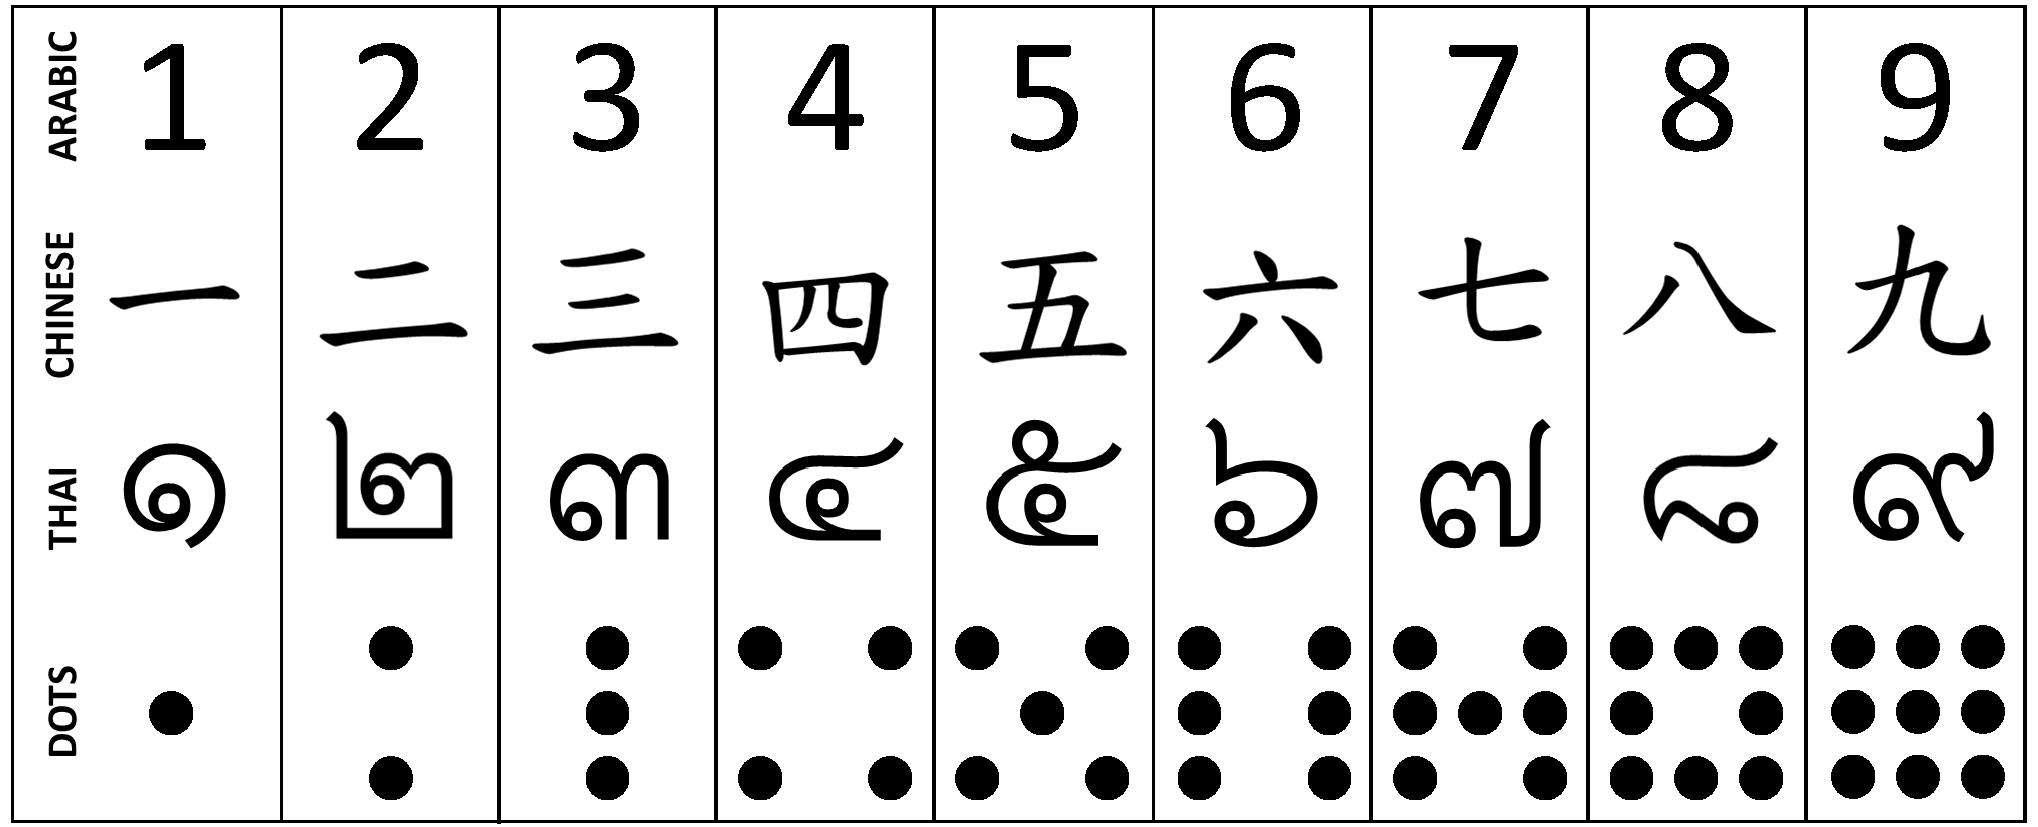
\includegraphics[width=\linewidth]{Figures/Wheel/NumStim.pdf}
\caption{Arabic, Chinese, Thai and dot numerals for the range of one to nine (left to right).}
\label{fig:Wheel_NumStim}
\end{figure}

Target stimuli were displayed in the center of the screen within a noisy field \cite<$\mu$ = 0, $\sigma$ = 0.125; à la>{eidels2014measuring} and were followed by a central backwards-mask. At a viewing distance of 60cm, each noisy target stimuli subtended a visual angle of 5.53 degrees (5.8cm$^2$) and the mask subtended a visual angle of 11.61 degrees (12.2cm$^2$). Responses were made by moving the mouse to the matching numeral presented within a response-wheel (see Figure \ref{fig:Wheel_SlideOrder}). The response-wheel was evenly divided into nine sectors, each containing one of nine numeric-symbols. The symbols were sampled from one of the four numeric-conditions (Arabic, Chinese, Thai and Dots; see Figure \ref{fig:Wheel_NumStim} again). Each numeral was randomly allocated to a wheel sector at the start of each session and displayed equidistant from the starting mouse location. This design ensured no one numeral was spatially biased towards the target.

At the start of each response-window, a mouse-cursor appeared in the center of the number-wheel. Participants responded by moving the mouse-cursor towards the segment that contained the best match to the previously presented stimulus. A response was taken once the cursor passed over the inner-circle of the response-wheel. At a viewing distance of 60cm, the inner-circle of the response-wheel subtended 20.04 degrees visual angle (diameter 21.2cm) and the outer-circle subtended 25.91 degrees visual angle (diameter 27.6cm). All experimental displays were presented on a gray background with RGB values (240, 240, 240). 

\subsection{Procedure}
Participants completed four 90min sessions --- Arabic, Chinese, Thai and non-symbolic dots. Session order was randomized using a Latin-square design. At the start of the first session participants were presented an information statement and provided signed consent before answering demographic questions regarding age, gender, handedness and vision. Participants reported whether they identified as being proficient in English, Chinese and Thai. At the start of each session participants were instructed to briefly view a noisy symbol, and using the mouse, identify the best matching symbol on the response-wheel.

Each trial began with a blank screen presented for 250ms, followed by a central fixation-cross for 500ms, followed by a 250ms blank screen. The stimulus display was then presented for 500ms, followed by a mask for 200ms. The response-window began at the presentation of the response-wheel and lasted 8000ms (see Figure \ref{fig:Wheel_SlideOrder}). A trial ended when a response was made or when the trial timed-out. 

% Trial Order Slide
\begin{figure}[tbh]
\centering 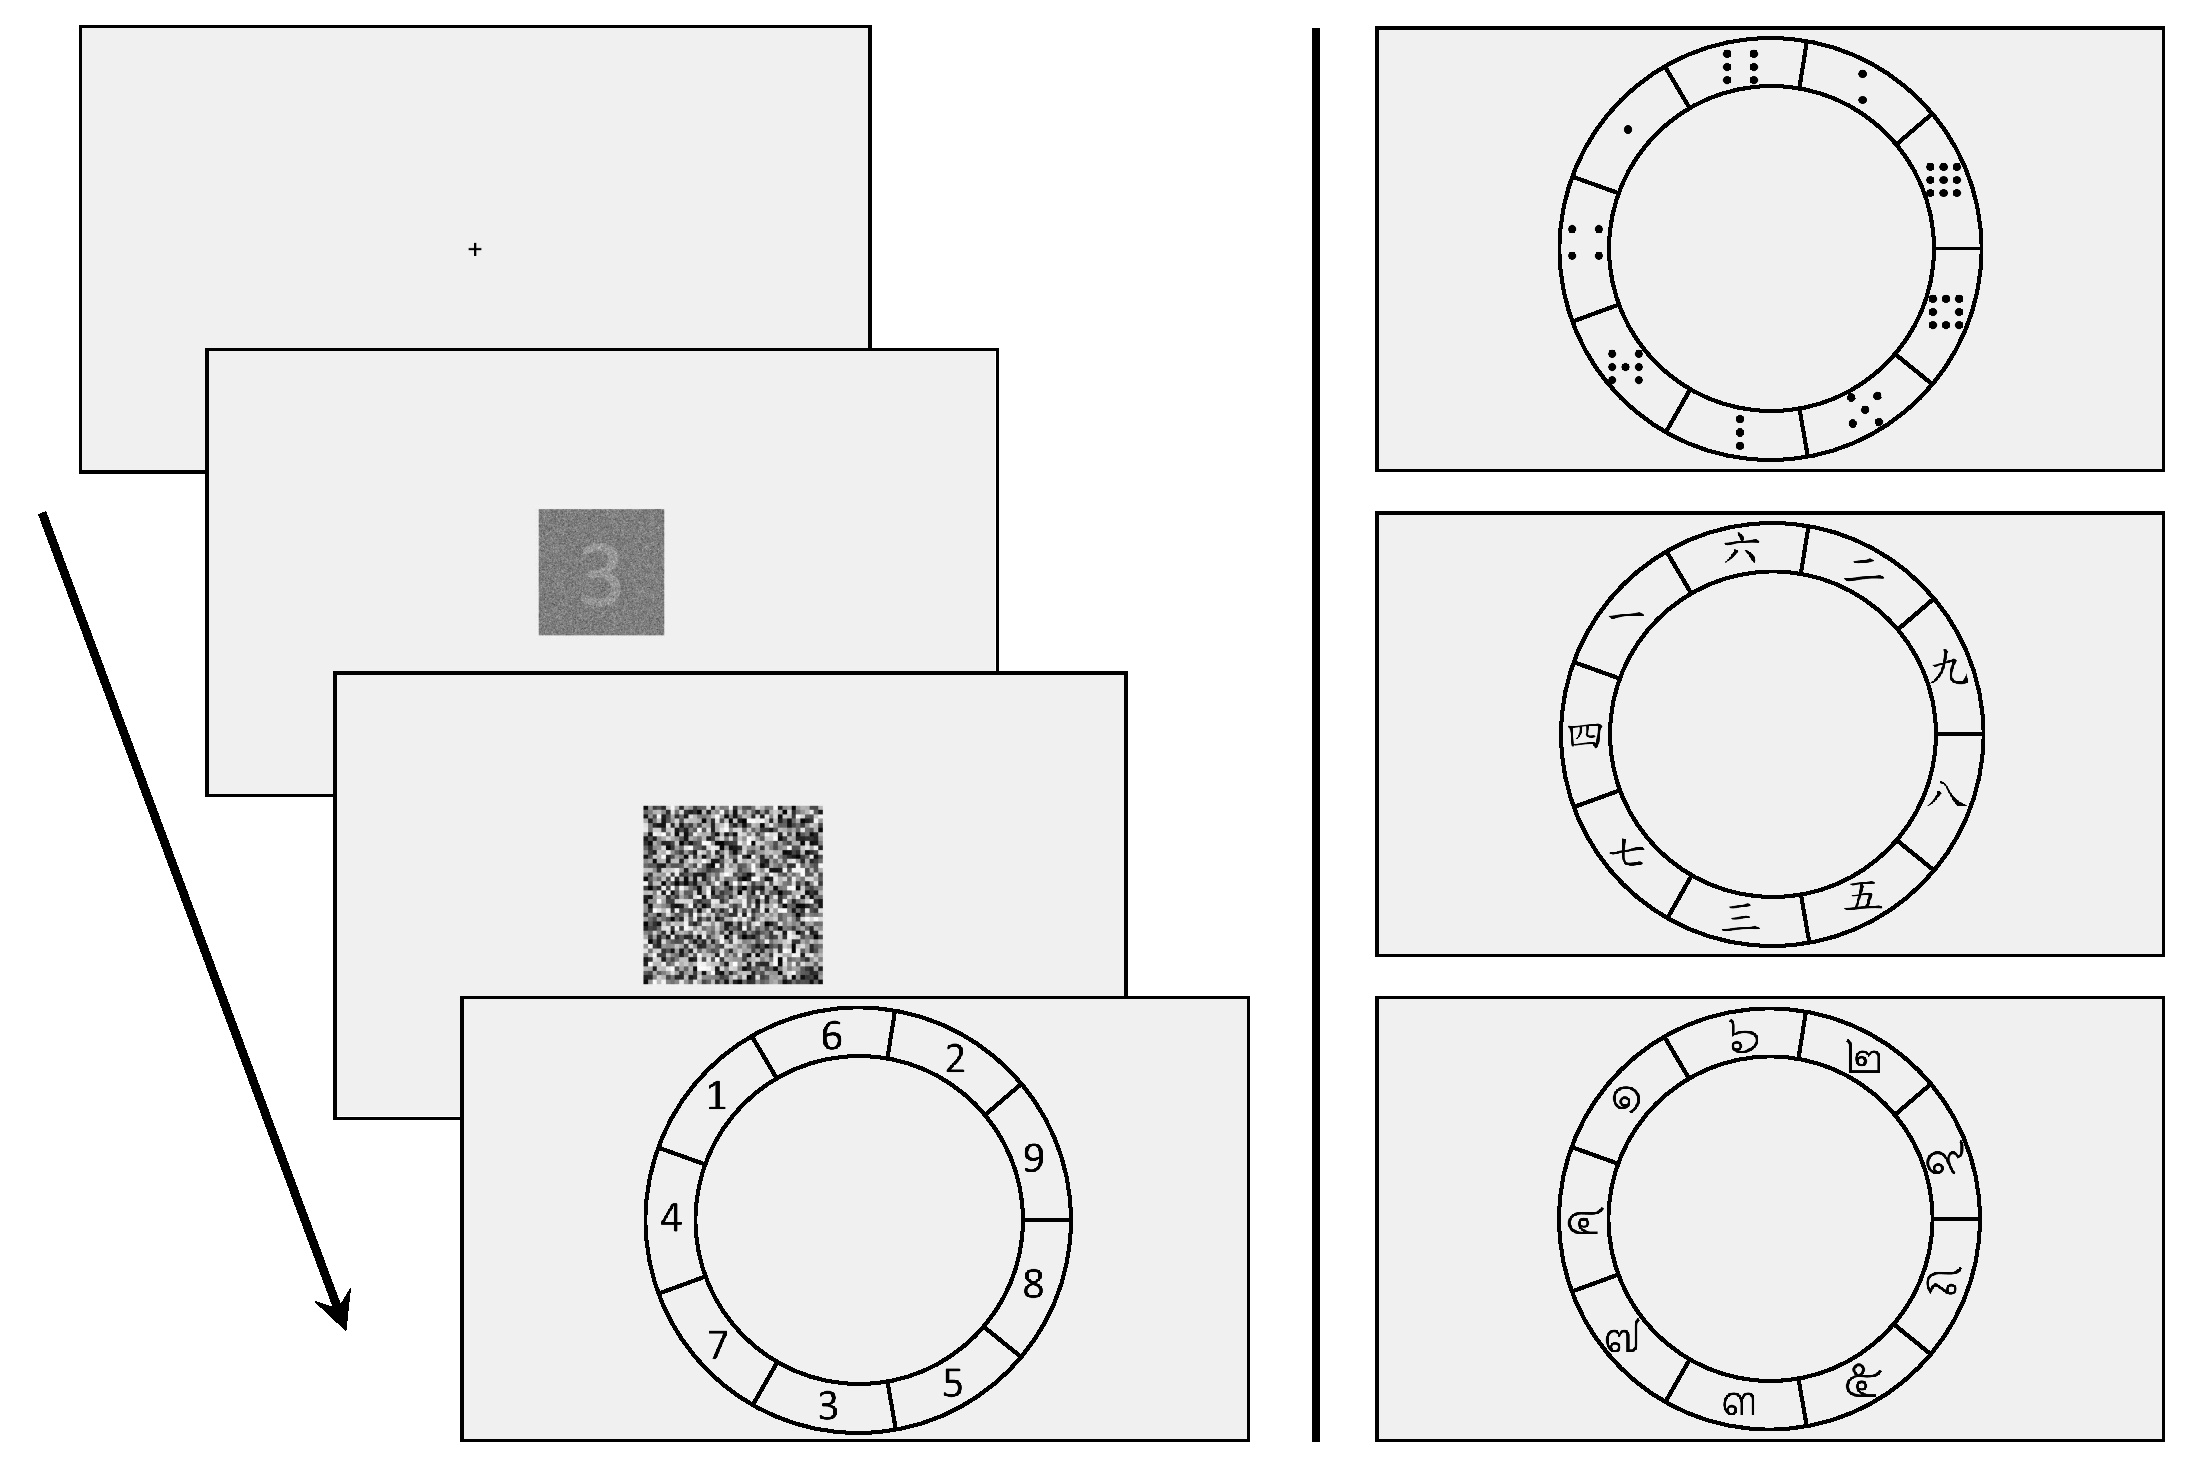
\includegraphics[scale = .37]{Figures/Wheel/TrialOrderSlide.pdf}
\caption{Illustration of a trial with Arabic numerals (left). Alternative response-wheels are displayed (right) for the non-symbolic dots (top), Chinese (middle) and Thai (bottom) numerals. For illustrative purposes, the position of each numeral is held constant between numeric-types.}
\label{fig:Wheel_SlideOrder}
\end{figure}

% Staircase Procedure
At the start of each session, participants completed a practice-calibration block. By means of a single staircase procedure, we manipulated the contrast of the signal across trials according to the participant's responses. A modified 2-up 1-down rule was applied\footnote{A classical 2-up 1-down staircase requires two correct responses on each step to step-up. Our modified staircase required a correct response on two contiguous trials, (\eg trial n-1 and trial-n), to step-up. This produced a faster and more responsive staircase procedure.}. Signal contrast began at a fixed RGB value (153, 153, 153), with two contiguous correct responses decreasing the RGB signal-values by 1 (becoming harder), and a single incorrect response increasing the RGB signal-values by 1 (becoming easier). This staircase design allowed participants to quickly plateau at their perceptual threshold. Earlier piloting with this procedure resulted in approximately 60\% accuracy in the main task. 

% Five Contrast Levels
Our proffered analysis technique, multidimensional scaling, requires a combination of correct and error responses. To ensure this, experimental stimuli were presented at five signal levels of varying difficulty \cite<following>{eidels2014measuring}. A critical contrast level was determined by the mean RGB values of the final 30 calibration trials. The highest signal level (easiest) was presented three RGB steps above the critical contrast. The lowest signal level (hardest) was presented one RGB step below the critical contrast. Together, these formed the five stimulus-signal contrast-levels. 

% Trials and Blocks
During each session, participants completed one practice block of 135 trials, and 13 experimental blocks each containing 90 trials. During an experimental block, each numeral was presented 10 times, twice at each of the five signal levels. Trial-by-trial accuracy feedback was provided during the practice-calibration block and trial order was randomized within each block. Block accuracy was displayed as a graph at the end of each experimental block to encourage participant engagement\footnote{At no point during the experiment were any numbers displayed except for those contained by the response-wheel and target-stimulus. Accuracy was presented as a line graph with no numbers, and countdown timer was displayed as a ticking sundial.}. In total, each participant completed 130 experimental trials per numeric-symbol, and 1170 experimental trials per-session. 

\subsection{Data Analysis}
Trials with no response were removed from the analysis. Calibration (practice) and experimental trials were assessed for accuracy to ensure an appropriately difficult stimulus-signal contrast was achieved. Repeated-measures ANOVAs and paired-sample \textit{t}-tests were used to statistically compare differences between numeric sets. Where accuracy was matched by signal-contrast level, between-subject ANOVAs and independent-samples \textit{t}-tests were used. Multiple comparisons were corrected for family-wise error using the bonferroni method.

For each participant, a 9 x 9 confusion matrix was generated for each numeric-type. To remove the effect of response-bias before MDS analysis, Luce's (1963) similarity choice model was applied to each confusion matrix. This model describes identification responses as probabilistic outcomes driven by the similarity of a stimulus to other in the choice set, as well as a response-bias parameter --- one for each stimulus. By estimating the parameters of the model, researchers can examine the theoretically meaningful similarity scores free from the effect of response-bias that can contaminate the observed data. In supplementary materials S4\ref{Appendix:Luce} we provide a formal description of Luce's choice model and describe the application to the current data. 

After application of Luce's choice model, non-metric multidimensional scaling was conducted on the bias-free similarity matrices. For each participant and each numeric-condition, a scree analysis was conducted to determine the appropriate number of MDS dimensions. Group MDS plots were generated for each numeric-type using the individual differences scaling (indscal) MDS technique \cite{carroll1970indscal}. Indscal provides a group MDS fit by deferentially weighting the contribution of each individual to the overall MDS fit. K-means cluster analysis was applied to determine cluster patterns at both the group level and across individuals. The frequency at which items clustered were turned into proportions and displayed as a heatmap, separately for each numeric-type. Finally, we compared MDS and K-mean cluster results to an ideal observer analysis, used to simulate pure perceptual confusions of the numeric sets.

\section{Results}
\subsection{Calibration Block}
Figure \ref{fig:Staircase} (top) depicts the calibration block for participant S1, responding to Arabic numerals. This staircase procedure was typical of all participants. The mean contrast level of the final 30 assessment trials (highlighted yellow) determined the critical contrast value --- the value from which stimulus-signal levels were determined in the experimental session. Violin plots (bottom) depict the mean and standard-error of contrast values for assessment trials, for each participant and numeric-type. Critical contrast levels were relatively stable across numeric-type and participants. 

% Staircase Figure
\begin{figure}[tbh]
\centering 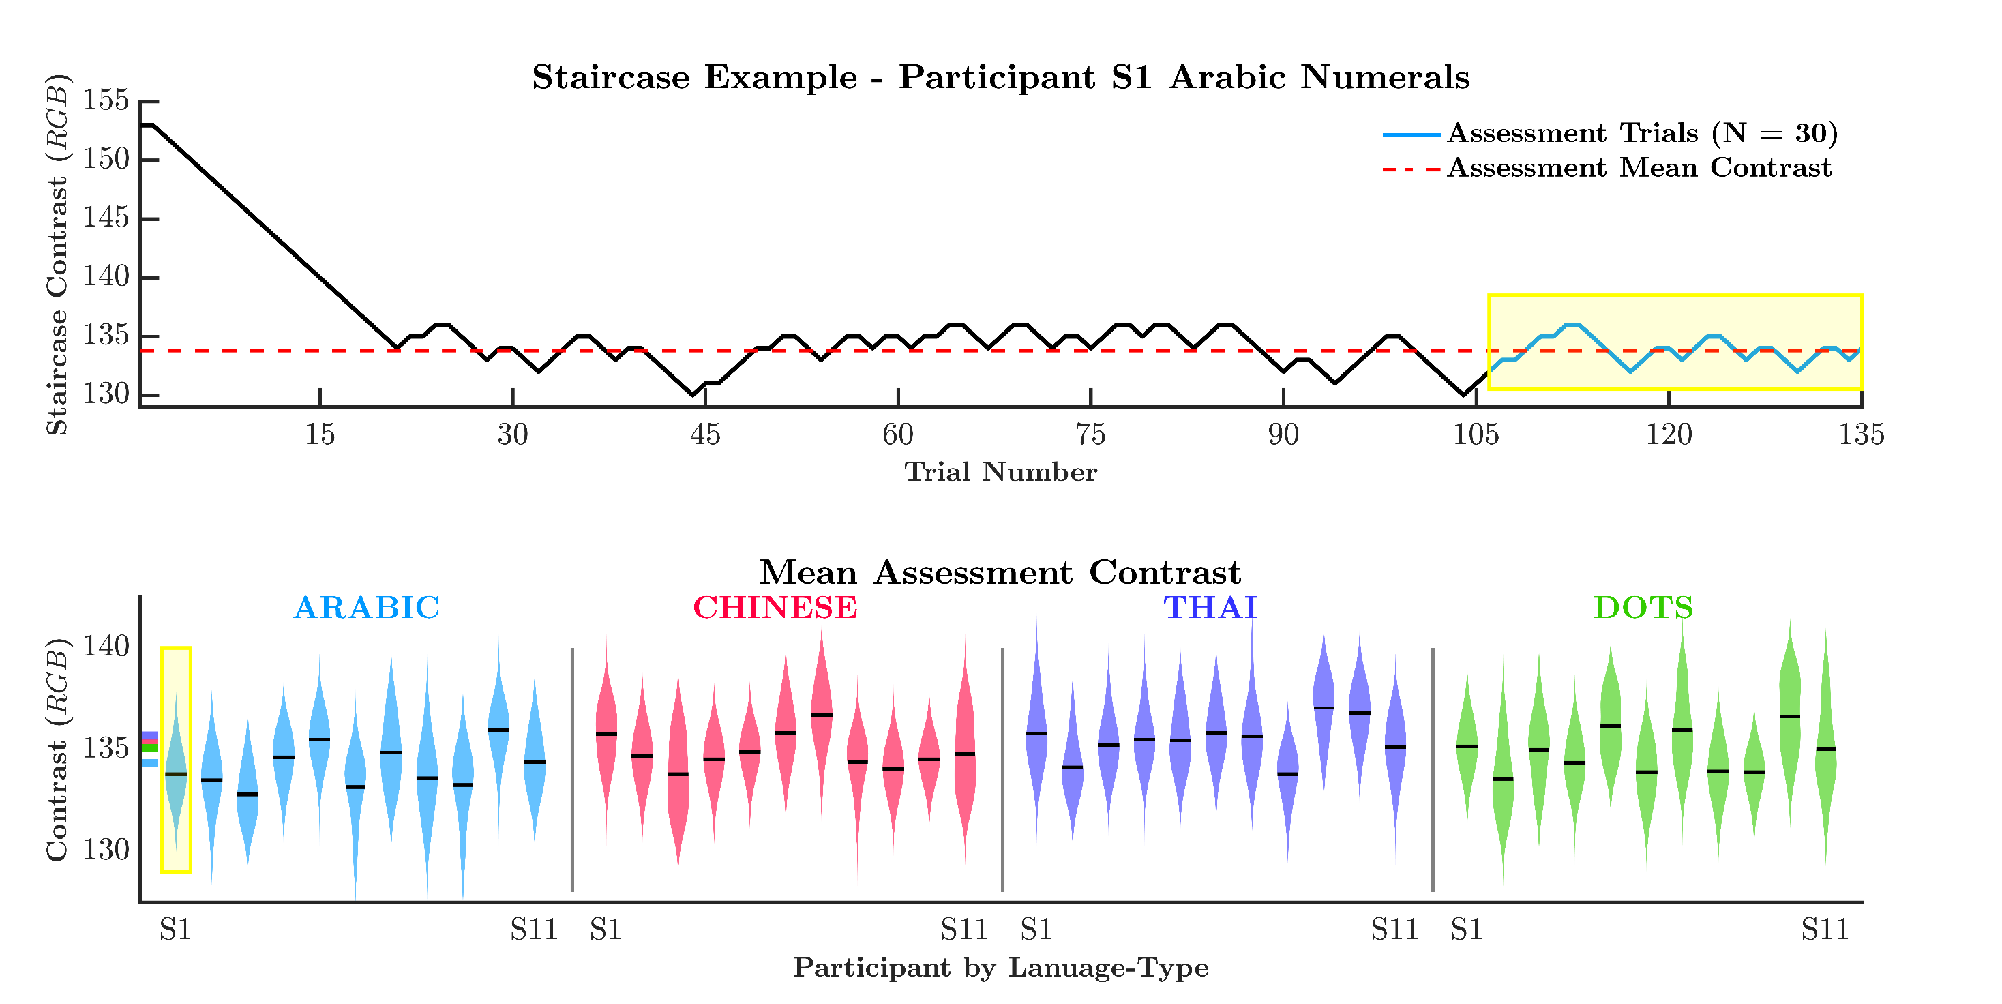
\includegraphics[width=\linewidth]{Figures/Wheel/Staircase.pdf}
\caption{Plot of participant S1's Arabic numeral staircase procedure (top) and violin plots of individual participant's staircase assessment trials (bottom). Assessment trials (highlighted yellow for participant S1) determined the critical contrast value for the main experiment. For all numeric-types, participants displayed relatively stable contrast levels during the assessment window. Black lines on each violin plot represents the critical contrast value (mean RGB value over the assessment window). Colored ticks on the y-axis are the mean critical contrast values for each numeric-type.}
\label{fig:Staircase}
\end{figure}

Colored ticks on the violin-plot (Figure \ref{fig:Staircase}, y-axis) show, on average, critical contrast levels were lowest for Arabic numerals (RGB $\mu$ = 134.14, $\sigma$ = 1.07), then non-symbolic dots (RGB $\mu$ = 134.88, $\sigma$ = 1.04), then Chinese numerals (RGB $\mu$ = 134.91, $\sigma$ = .86) and finally, Thai numerals (RGB $\mu$ = 135.5, $\sigma$ = .97). A lower signal-level suggests familiar numeric sets (Arabic and Dots) were easier to recognize than unfamiliar numeric sets (Chinese and Thai). However, the greatest difference between contrast levels, Arabic vs Thai, was only equivalent to a single RGB step.

\subsection{Experimental accuracy}
The staircase procedure was effective at reducing identification accuracy during experimental trials. On average, accuracy was highest for Chinese numerals ($\mu$ = .60, $\sigma$ = .21), then Arabic ($\mu$ = .59, $\sigma$ = .19) and non-symbolic dots ($\mu$ = .59, $\sigma$ = .19), and finally, Thai numerals ($\mu$ = .54, $\sigma$ = .19). Our manipulation of contrast accuracy was similarly effective. During experimental trials, stimuli were presented at five signal-levels, one step below the critical contrast value (level 1: hardest), at the critical value (level 2) and three steps above (levels 3, 4 and 5; easiest). As intended, mean accuracy increased linearly with the visibility of the contrast levels, being lowest at level 1 ($\mu$ = .32, $\sigma$ = .02) and highest at level 5 ($\mu$ = .80, $\sigma$ = .03). A full analysis of accuracy over contrast levels is provided in supplementary materials S4\ref{Appendix:contrastAcc}. For now, we  summarise by stating our manipulation of contrast worked as intended and produced error rates sufficient for our subsequent analyses.


\subsection{Response Bias}
Figure \ref{fig:AccRspFq}.a. shows the positive relationship (rank-order correlation $\rho$ = .83***) between response-frequency (blue) and response-accuracy (orange) for Arabic numerals in participant S1. Here, as the frequency of responding with a specific numeral, for example `4', increases, so too does identification accuracy. Similarly, as response-frequency decreases, such as with item `3', accuracy also decreases. This figure clearly displays the relationship between response-frequency (`strength' in Luce's choice model) and response-accuracy. 

The dotted blue line in Figure \ref{fig:AccRspFq}.a represents a response-frequency matching the number of stimulus presentations. For example, a `5' response was made as often as `5' was presented, however, these responses were correct only half of the time. By contrast, a `4' response was made nearly twice as often as it was presented, showing an effect of response-bias. The positive relationship between response-frequency and response-accuracy is evident when we examine the scatter plot in Figure \ref{fig:AccRspFq}.b. This scatter plot depicts accuracy against response-frequency (bias) for each participant, for each stimulus and numeric-type. The positive relationship ($r$ = .58***) indicates that in a standard analysis, overall accuracy and response bias could be mistakenly conflated. This highlights the need for a bias free measure of similarity, as offered by Luce's choice model.

\begin{figure}[tbh]
\centering \includegraphics[width = \linewidth]{Figures/Wheel/AccuracyResponseFreq.jpg}
\caption{a) Response frequency by response accuracy for participant S1, Arabic numerals. b) Scatter plot depicting a positive correlation between mean stimulus accuracy and response frequency, across numeric-types. c) Response frequency by response accuracy for stimuli for the Arabic (left), Chinese (mid-left), Thai (mid-right) and Dot (right) numeric-types.}
\label{fig:AccRspFq}
\end{figure}

Figure \ref{fig:AccRspFq}.c shows the mean response-frequency and mean response-accuracy of each stimulus, separately for each numeric-type. Averaging response-frequency and accuracy diminishes their correlation, however, clearly illustrates response patterns and accuracy for each stimulus. Together, these results show how an increase in response-frequency (or strength in Luce's choice model) can artificially improve identification accuracy for any given stimulus. Similarly, these results show how a decrease in response-frequency can lead to poorer stimulus identification accuracy. To understand the impact response-bias has on confusion data and our analysis of the mental space, we now consider our MDS results.

\subsection{Multidimensional Scaling}
\subsubsection{Response bias}
Figure \ref{fig:Bias2Unbias} shows MDS results from a representative data set (participant S4)  where response-bias was unaccounted for (biased plots) and corresponding MDS results where response-bias was removed from the data using Luce's choice model (bias-free plots). Changes between item-proximity within each numeric-type (blue arrows) illustrates how response-bias alters the MDS solution. All future references to MDS within the results section will pertain to the bias-free MDS solutions.

\begin{figure}[tbh]
\centering \includegraphics[scale = .48]{Figures/Wheel/BiasToUnbiasSingle.jpg}
\caption{Biased (uncorrected) and bias-free (Luce's choice model corrected) MDS solutions for participant S4, displayed separately for each numeric-type. Changes in item-proximity between biased and bias-free MDS plots displays the influence of response-bias on the MDS solution. \\\textbf{Note.} Numerals displayed within the MDS plots are for illustrative purposes and are not identical to the experimental stimuli; see Figure \ref{fig:Wheel_NumStim}. Dots are presented as Arabic numerals to avoid misinterpretation where numerals spatially overlap.}
\label{fig:Bias2Unbias}
\end{figure}

Scree analysis identified two-dimensions as an appropriate MDS representation for most participants in each of the four numeric-types (for more details see supplementary materials S4, Figure \ref{fig:Apx_ScreeEngDot} and Figure \ref{fig:Apx_ScreeChnThi}). Scree analysis identified three-dimensions as the appropriate MDS representation for three participants in the Arabic and Thai numeric-types, and the appropriate representation for four participants in the Chinese numeric-type. Individual bias-free MDS plots are displayed in supplementary materials S4, Figure \ref{fig:Apx_MDSenglish} -- Figure \ref{fig:Apx_MDSthai}; biased MDS plots are displayed in supplementary materials S4, Figure \ref{fig:Apx_MDSenglishBiased} -- Figure \ref{fig:Apx_MDSthaiBiased}). To describe trends observed across participants, we conducted an Individual Differences Scaling (indscal) MDS analysis. Results of the three-dimensional MDS indscal solutions (see supplementary material S4, Figure \ref{fig:Apx_3D_Indscal}) closely resemble the results of the two-dimensional MDS solutions. For efficiency of exposition, the following will focus on the majority of participants and the two-dimensional indscal results.

\subsubsection{MDS indscal interpretation}
Figure \ref{fig:Indscal} displays the group MDS indscal solutions for data collapsed across those participants best represented by two-dimensions, separately for each numeric-type. Interpretation of MDS plots is at times arbitrary and relies on visual inspection of the plots. Similarly, interpretation of the MDS solution's axes are also arbitrary with reference to the x- or y-axes \cite<see e.g.,>{nosofsky1986attention, nosofsky2018toward}. Likewise, the notion of similarity is very broad and has been the centre of many disputes in the literature \cite<e.g.,>{tversky1977features, medin1993respects}. We begin with a visually-guided assessment of the MDS plots, and then move to more formal analyses of clustering (using K-means cluster analysis) and similarity (using a rudimentary yet useful ideal-observer analysis). 

Arabic numerals appear to be arranged along dimensions of roundness (x-axis) and openness \cite<y-axis; similar results were observed by>{godwin2014numSim}. Arabic numerals formed four groups in the MDS space: [2,7], [1,4], [5,6] and [3,8,9]. The dimension of openness best described the diagonal of the y-axis\footnote{The rotation and direction of items within the MDS solution, relative to the x- and y-axis, is arbitrary. It is only important that these dimensions are orthogonal to one-another.} for all numerals except the closed shape of item `8'. Under noisy stimulus conditions, the concave exterior of `8' might be perceived as more `open' than it would under ideal viewing conditions. These results show an apparent effect of perceptual similarity on the mental representations of Arabic numerals.

\begin{figure}[tbh]
\centering 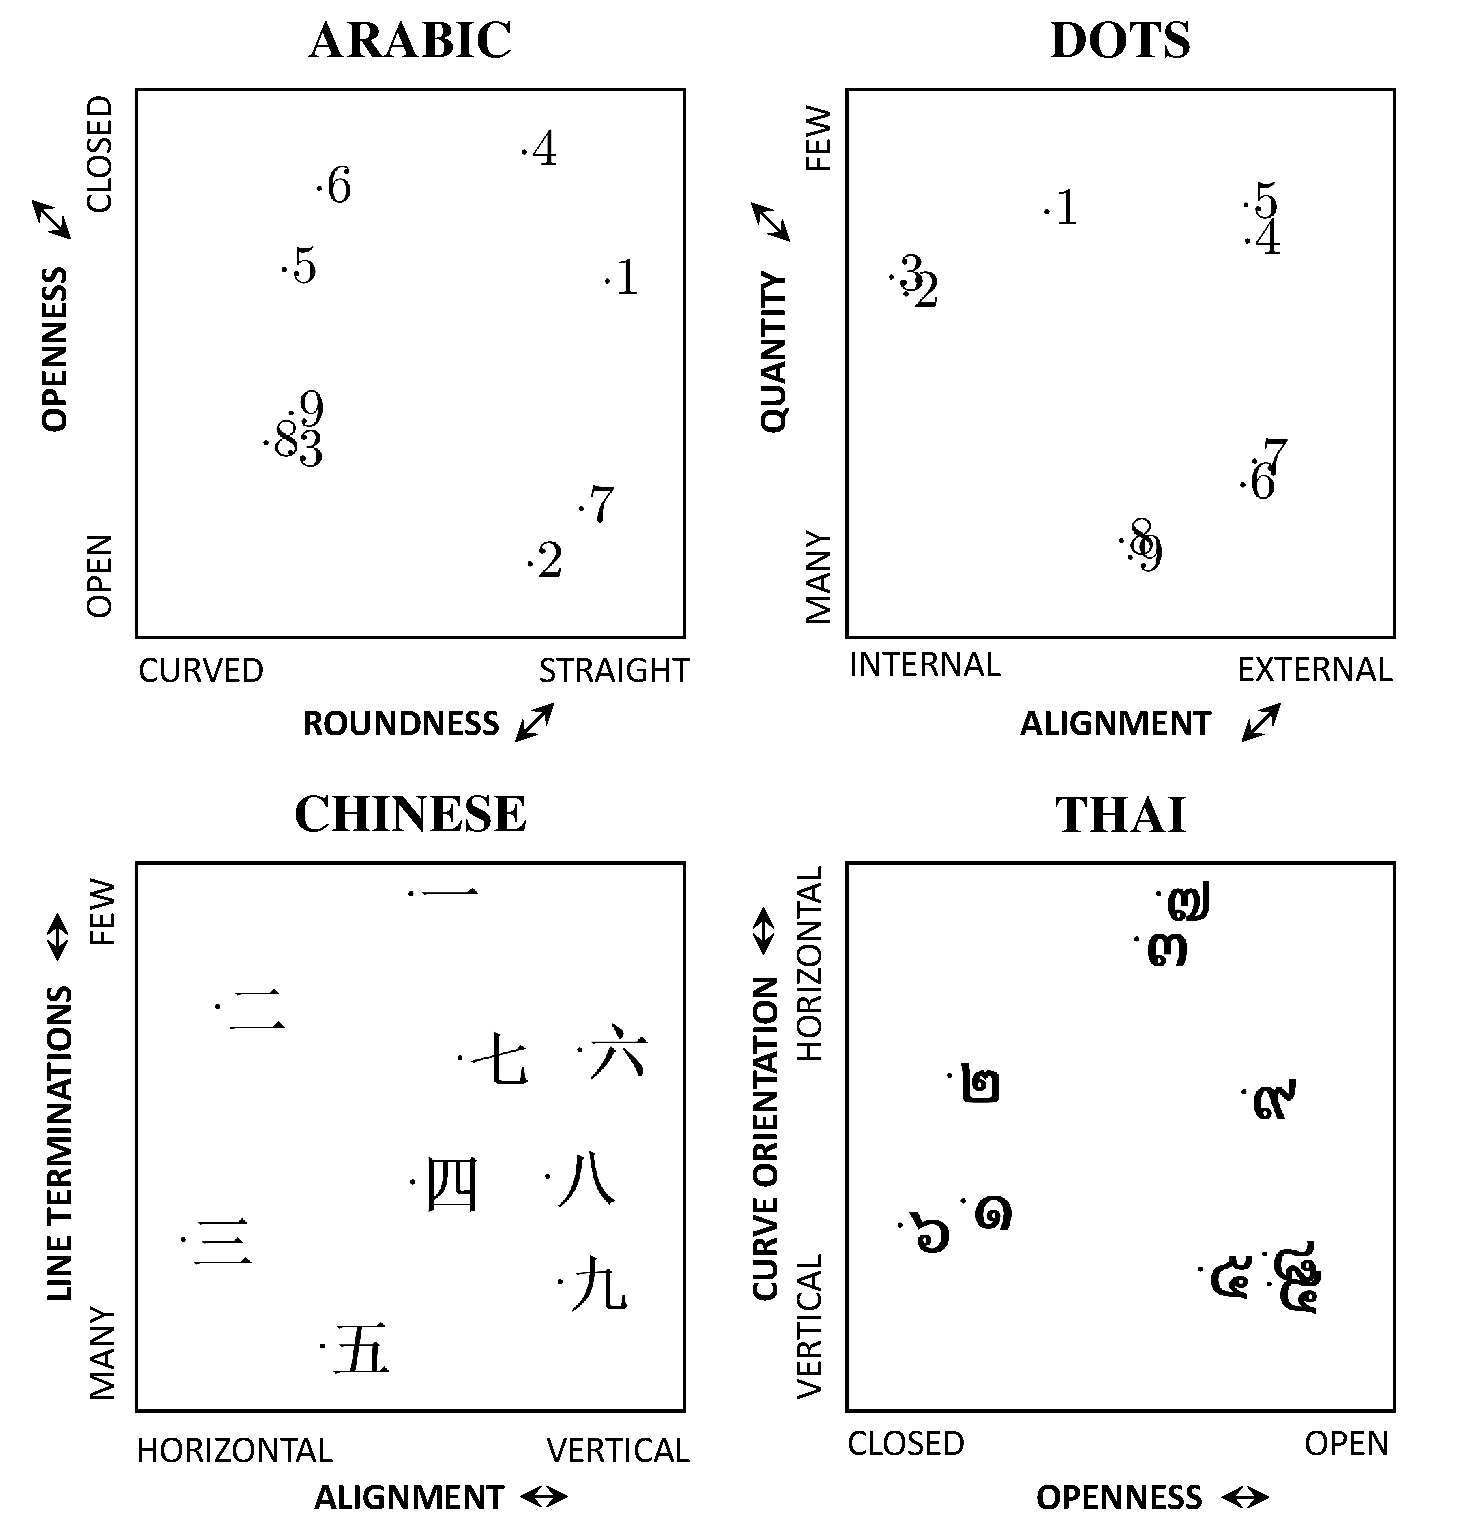
\includegraphics[scale = .45]{Figures/Wheel/IndscalDescription.pdf}
\caption{Individual differences scaling (indscal) solution for all participants best represented by a two-dimensional MDS space, displayed separately for each numeric-type. Dimensional labels and directionality (arrows) are displayed on the y-axis and x-axis.}
\label{fig:Indscal}
\end{figure}

The non-symbolic dots indscal MDS solution (Figure \ref{fig:Indscal}) appears to be displayed across dimensions of alignment (x-axis; whether items are presented internally or externally in the nine-dot array) and quantity (y-axis). Non-symbolic dots show five distinct groupings: [1], [2,3], [4,5], [6,7], [8,9]. These groupings suggest items cluster by numerical proximity. Furthermore, if we ignore the unique case of one-dot, numerical magnitude increases in a clock-wise direction, possibly reflecting the mental number-line. These results show an apparent effect of numerical magnitude and perceptual similarities on the mental representations of non-symbolic dots. 

The Chinese indscal MDS solution (Figure \ref{fig:Indscal}) appears to be arranged across dimensions of alignment (x-axis) and line terminations (y-axis). Chinese numerals are logographic, a trait captured by the visual property of alignment. As a consequence, small-magnitudes and large-magnitudes are mostly separate within the MDS space. Within this space, the Chinese numerals show three distinct groupings, \begin{CJK}{UTF8}{gbsn} [一, 二], [三, 五] and [四, 六, 七, 八, 九].\end{CJK} It is unclear whether the largest group might be better classified as two or three sub-groups, for example, \begin{CJK}{UTF8}{gbsn} [四], [六, 七] and [八, 九].\end{CJK} These results show an apparent effect of perceptual similarity on the mental representations of Chinese numerals.

The Thai indscal MDS solution (Figure \ref{fig:Indscal}) appears to be arranged across dimensions of openness (x-axis) and curve orientation (y-axis; \ie whether item curvature is horizontally or vertically aligned). Thai numerals show four distinct groupings: numerals with a vertical curve (numerals [3, 7]), numerals with a horizontal curve (numerals [4, 5, 8]), numerals with a closed shape (numerals [1, 2, 6]), and the solo group of item nine. These results show a clear effect of perceptual similarity on the mental representations of Thai numerals. 

Based on visual inspection, indscal MDS solutions provided an accurate representation of individual participant MDS results. Arabic, Chinese and Thai numerals were represented within the mental space across dimensions of perceptual similarity. Non-symbolic dots were represented within the mental space using dimensions of numerical and perceptual similarity. Indscal analysis is useful for identifying latent MDS dimensions, however, does not provide a formal measure of item-clustering. 

Deciding which items group together and which items are independent is a difficult process. For example, visual inspection of the Arabic indscal solution suggests items `1' and `4' may cluster together or may be independent. Similarly, Chinese numerals \begin{CJK}{UTF8}{gbsn}[四, 六, 七, 八, 九]\end{CJK} may form one group, or three. The `strength' with which two numerals cluster, may determine the likelihood of their confusion within the mental space. To characterize the strength of item-clusters in each individual, and across two- and three-dimensional MDS solutions, we applied to the data a variant of K-means clustering analysis. 

\subsection{MDS clustering}
K-means is an iterative clustering technique used to identify item groupings within dense data sets. A number of randomly located centroids (K) are updated iteratively until the data set can be partitioned into `K' non-overlapping clusters. This method works well for large, dense data sets, however, experiences a notable limitation with small data-sets.

Identifying the correct number of centroids is difficult for small data sets. Two, three or four centroids may be adequate for a sample of nine items. However, cluster selection methods developed for large data sets will generally favor higher centroid counts, (\eg five or six centroids), at a risk to over-fitting the data. 

To overcome this limitation, we ran K-mean cluster algorithms using 2--6 centroids, on each bias-free MDS solution. On each iteration of `K', we recorded which items clustered together (Figure \ref{fig:Kmean}.a) to produced a measure of cluster frequency (Figure \ref{fig:Kmean}.b). For illustration, in the data presented in Figure \ref{fig:Kmean}.b, the digits '1' and '2' were clustered together three times (across the the fine clustering scenarios, K=2, K=3, ... K=6, illustrated in Figure \ref{fig:Kmean}.a), whereas the digits '1' and '4' were clustered together only one time. Of course, each digit is always clustered with itself, resulting in the maximum value of five along the main diagonal.

Within each numeric-type, cluster frequencies were summed across participants and represented by proportion (see Figure \ref{fig:HeatMapSubjects}.a). Separate heatmaps were calculated for two-dimensional and three-dimensional participants (supplementary material S4, Figure \ref{fig:Apx_2D_MDScounts} -- Figure \ref{fig:Apx_3D_MDScounts}). Being comparable, these results were collapsed into Figure \ref{fig:HeatMapSubjects}.a. This method was robust to the number of MDS dimensions, as clusters could be calculated in either two- or three-dimensional space. For direct comparison to the previously presented group indscal results, a separate cluster heatmap was generated using the two-dimensional indscal results (Figure \ref{fig:HeatMapSubjects}.b).

% Kmean Cluster Explainer
\begin{figure}[tbh]
\centering \includegraphics[scale = .45]{Figures/Wheel/ClusterExplainer.jpg}
\caption{a) K-mean cluster solutions for 2--6 clusters, for a single participant. K-mean cluster centers (centroids) are illustrated by `x' markers, and groupings are denoted by color. b) Cluster frequency heatmap for the same data. Darker colors indicate items which most frequently cluster together.}
\label{fig:Kmean}
\end{figure}

% Participant Response - Item Clusters
\begin{figure}[tbh]
\centering 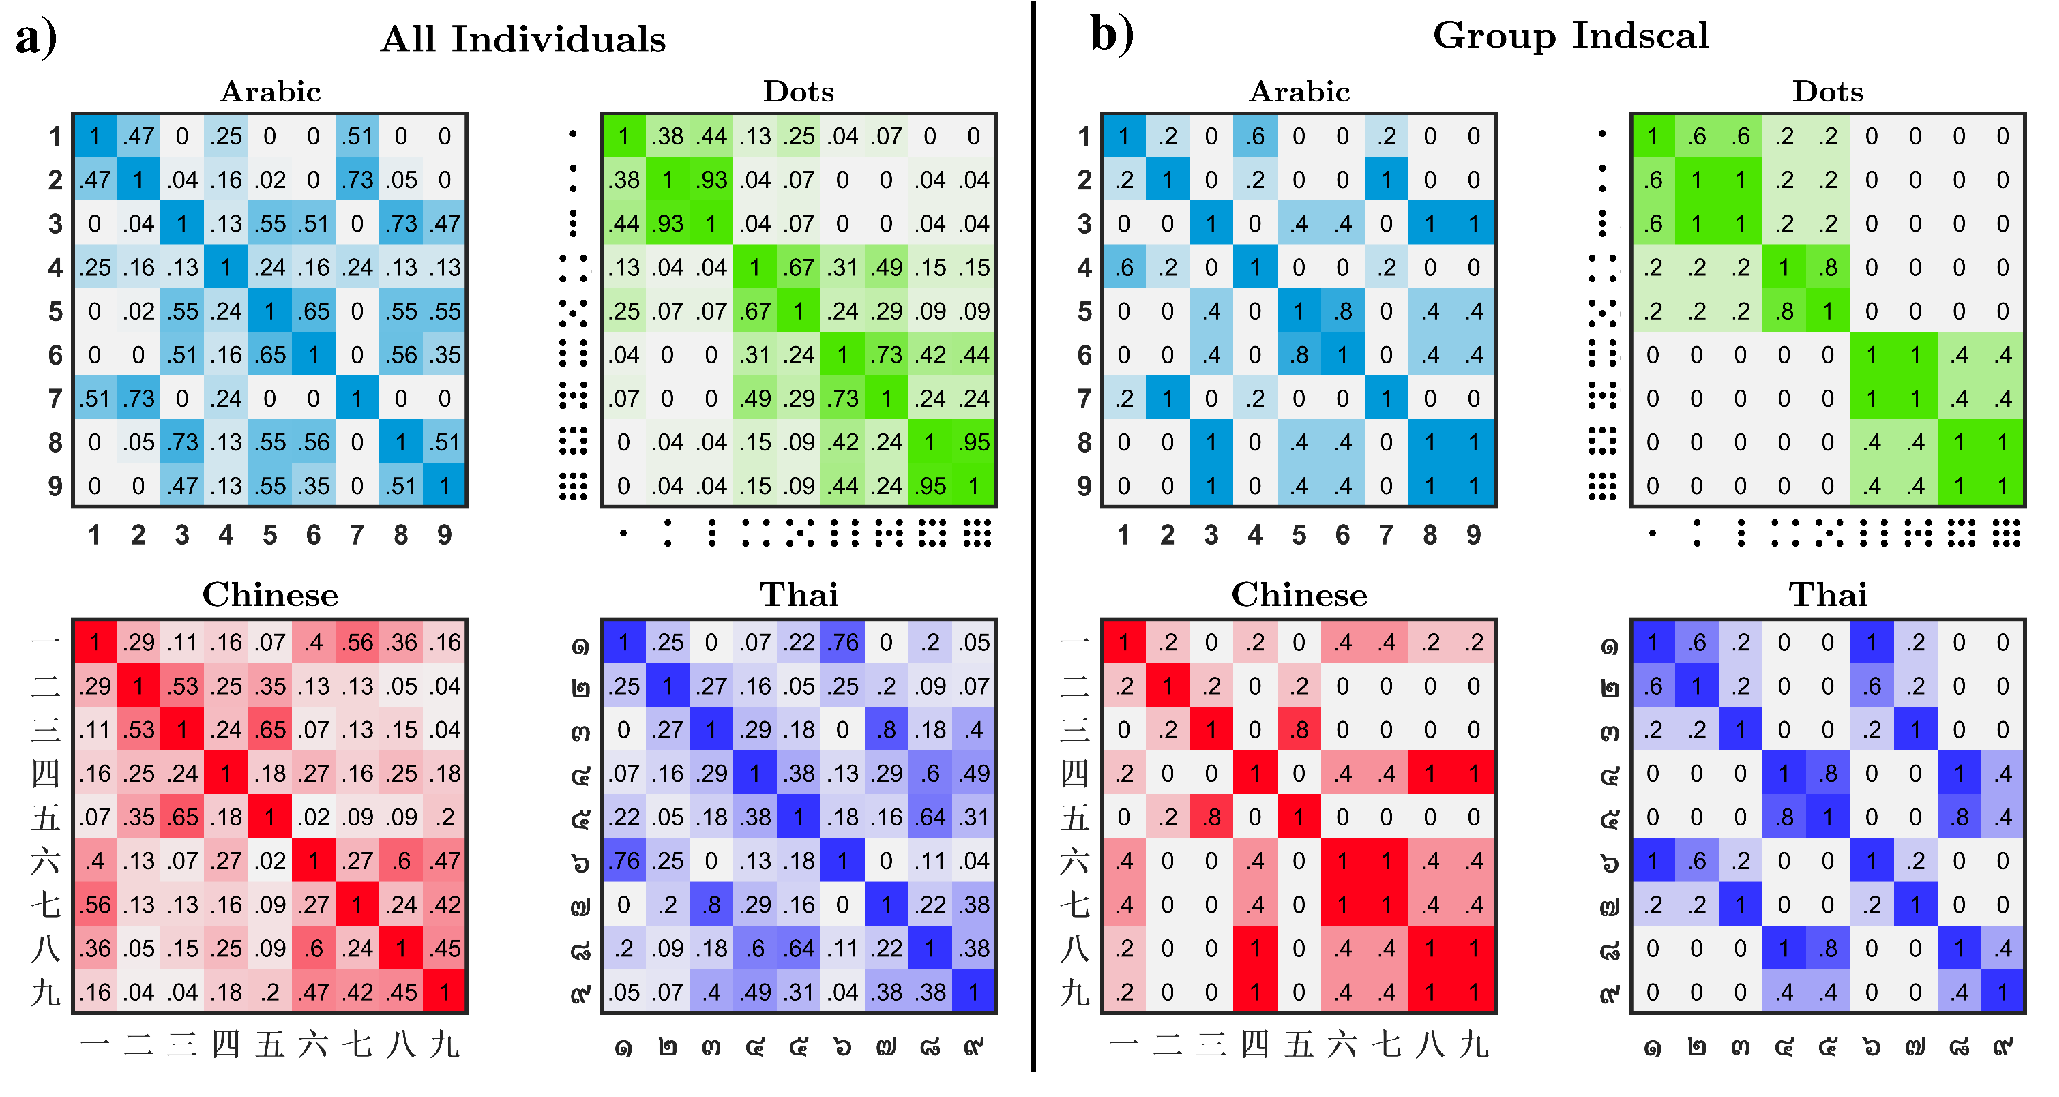
\includegraphics[width=\linewidth]{Figures/Wheel/IndivVsIndscalHeatmap.pdf}
\caption{a) Proportional cluster-frequency heatmap for all eleven participants (including both two- and three-dimensional MDS solutions), across 2--6 K-mean clusters. b) Group indscal two-dimensional MDS (Figure \ref{fig:Indscal}) cluster-frequency heatmap, across 2--6 K-mean clusters. Larger proportions (darker colored squares) indicate items which most frequently cluster together.}
\label{fig:HeatMapSubjects}
\end{figure}

% Arabic Clusters
The top-left of Figure \ref{fig:HeatMapSubjects}.a displays the proportion by which items clustered across individuals, for Arabic numerals. Across individuals, the strength of items clusters generally aligned with the group indscal results (top-left, Figure \ref{fig:HeatMapSubjects}.b). In line with the indscal MDS solution, items with similar perceptual properties, for example, the items [3, 5, 6, 8, 9] share the perceptual property of `roundness', while [2, 3] share the property of `openness'; frequently clustered across individuals. Cluster patterns displayed no effect of numerical proximity (neighbouring items clustered infrequently). These results support the indscal analysis, and suggest that at the individual level, Arabic numerals were clustered strongly by the perceptual properties of `curvature' and `openness'. 

% Dot Clusters
The top-right panel of Figure \ref{fig:HeatMapSubjects}.a displays the proportion of item-clustering for non-symbolic dots. The left-to-right diagonal pattern of results, radiating outwards towards zero in the opposite corners, suggests items clustered by numerical proximity. Yet, items close in numerical proximity cluster together in staggered item-sets. For example, items [2, 3], [4, 5] and [6, 7] cluster, but rarely [3,4], [5,6] or [7,8]. This pattern of results is made clearer by the group indscal plot (Figure \ref{fig:HeatMapSubjects}.b). This staggered pattern of results is not accounted for by numerical proximity, but rather, perceptual similarities. 

% Staggered Dot Clusters
Staggered clusters, such as 4 and 5 dots, share similar perceptual characteristics, and differ only by the location of a single, central dot. Mental distance between dot representations are likely confounded by both perceptual similarity and numerical proximity; minimal changes such as adding one dot result in minimal changes to both quantity and visual appearance, and likewise adding a large number of dots to a display results in substantial changes to both quantity and visual appearance. As such, it could be that our observed clusters are due to i) only perceptual, ii) perceptual \textit{and} numerical, or iii) only numerical similarities. Results from the indscal MDS solution suggested items were confused along dimensions of quantity (numerical) and alignment (perceptual). As such, it seems likely this staggered pattern reflects a combination of numerical and perceptual similarities.

% Chinese Clusters
The bottom-left panel of Figure \ref{fig:HeatMapSubjects}.a displays cluster frequencies for Chinese numerals across individual participants. These results do not align with numerical-proximity, (\eg non-symbolic dots heatmap), and suggests items clustered by perceptual similarity. Noisy, low-frequency item-clusters are common for Chinese numerals, reflecting the unfamiliar nature of this numeric set with our cohort. Moderate cluster frequencies are present between numerals \begin{CJK}{UTF8}{gbsn} [二, 三, 四, 五] and [六, 七, 八, 九]\end{CJK}. The items within these groups are --- unbeknownst to our participants --- numerically contiguous. This clustering might reflect the logographic nature of the Chinese numeric-set and the perceptual similarities within smaller and larger magnitudes. 

% Chinese clusters - perceptual
With increases in magnitude, Chinese numerals shift from horizontal to vertical alignment, creating perceptual similarities within smaller and larger magnitudes. Furthermore, smaller magnitudes are generally represented by fewer line-features, (\ie line-endings), than larger magnitudes. Subsequently, perceptual similarities are strongest within smaller and larger magnitudes. This accounts for the observed indscal MDS results (Figure \ref{fig:HeatMapSubjects}.b) and cluster frequency results. Together, these analyses suggest that at the individual level, Chinese numerals are strongly influenced by the perceptual properties of `alignment' and `line-endings'. 

% Thai Clusters
The bottom-right panel of Figure \ref{fig:HeatMapSubjects}.a displays cluster frequencies for Thai numerals. Similar to Chinese numerals, Thai cluster patterns do not align with numerical proximity and display an abundance of low-frequency clusters. This may reflect the unfamiliar nature of the numeric-set. Across individuals, and at the group level (Figure \ref{fig:HeatMapSubjects}.b), high cluster frequencies are apparent between item numbers [1,6], [3,7], [4,8], [4,5] and [5,8]. Notably, these items share perceptual features of `roundness' and `curvature orientation'. Supplementing these findings with the previous indscal MDS analysis, results suggest that at the individual level, Thai numerals clustered strongly by the perceptual properties of `curvature orientation' and `roundness'. 

% Summary of Cluster Results
Supplementing indscal analysis with cluster frequency heatmaps, our results indicate perceptual similarity strongly influenced the confusion of Arabic, Chinese and Thai numerals. Furthermore, perceptual similarity also influenced the confusion of non-symbolic dots, but could be confounded with numerical distance in this set, as explained above. Determining the fidelity of these claims is difficult without a benchmark model for comparison. To this end, we now present simulated results from a simple ideal observer analysis. 

\subsection{Ideal Observer Analysis}
% IOA Method
The ideal observer analysis is a simple template matching process that compares numeric stimuli, pixel-by-pixel, to generate a confusion matrix. The ideal observer is $not$ a model of human performance, but rather, a benchmark against which we may compare the performance of human observers \cite<\eg>{gold1999identification, eidels2014measuring}. The `ideal observer' compares a noisy numeric stimulus to all possible templates, for example comparing a noisy `1' stimulus to the numerals `1--9'. The template with the best cross-correlational match over many iterations, with randomly sampled noise, is selected as the `ideal observer response'. Normally distributed noise ($\mu$ = 0, $\sigma$ = [1.065, .12, 1.127, 1.463] for Arabic, dot, Chinese and Thai numerals, respectively) is added to each numeric stimulus, until the ideal observer's accuracy resembles the average accuracy of the participants. This process was repeated 10,000 times, per numeric-stimulus, per numeric-type, generating four confusion matrices. 

% IOA Figures
To afford a direct comparison to the collected participant data, Luce's choice model was applied to the simulated ideal observer data. Figure \ref{fig:IOA}.a displays the bias-free MDS solutions generated by the ideal observer. Figure \ref{fig:IOA}.b displays the corresponding K-mean cluster frequency heatmaps. These Figures provide a benchmark of performance, given numeric-stimuli were only confused by perceptual similarities.

% Figure: IOA MDS and Heatmap 
\begin{figure}[tbh]
\centering \includegraphics[scale = .4]{Figures/Wheel/IOA2.jpg}
\caption{a) Ideal observer analysis bias-free MDS solutions, generated separately for each numeric-type. Non-symbolic dots are displayed as Arabic numerals in the MDS plot for clarity to the reader. b) Ideal observer K-mean cluster frequency heatmaps.}
\label{fig:IOA}
\end{figure}

% IOA vs Arabic
Comparing Arabic indscal MDS results (Figure \ref{fig:Indscal}.a) to the Arabic ideal observer MDS results (Figure \ref{fig:IOA}.a), we observe differences between item proximities and co-occurring item groups [2, 7] and [5, 6]. Comparing cluster frequency heatmaps, we find co-occurring item-clusters [1, 2], [2, 7], [5, 6], [5, 9] and [6, 9], suggesting participants confused these items due to perceptual similarities. Other item-clusters did not co-occur even though Arabic numerals appeared to be confused along dimensions of perceptual similarity.

% IOA vs Dots
Indscal MDS results for non-symbolic dots differed greatly from the ideal observer, and only shared item groups [1, 5] and [6, 7]. Cluster frequency heatmaps were comparable for items [1, 3], [6, 7] and [6, 8], yet the remaining item clusters were markedly different. Participants appeared to represent non-symbolic dots along dimensions of perceptual \textit{and} numerical similarity. The differences between participant and ideal observer MDS and cluster frequency results may reflect the impact of numerical proximity on the mental space. 

% IOA vs Chinese
The Chinese indscal MDS solution shared similarities with the ideal observer MDS solution. Chinese numerals \begin{CJK}{UTF8}{gbsn} [一, 二, 七], [三, 五], [四, 九] \end{CJK} group in both participant and ideal observer MDS solutions. Cluster frequency heatmaps were similar for items \begin{CJK}{UTF8}{gbsn} [一, 六], [二, 三], [四, 九], [四, 六], [四, 六] and [六, 七] \end{CJK}; these items all share distinct horizontal line features. While many item clusters were observed in both participant and ideal observer results, the pattern consistent with a logographic numeric-set was not observed by the ideal observer. As with our comparison of Arabic numeral results, it appears the ideal observer is only sensitive to a limited set of perceptual similarities.

% IOA vs Thai
The Thai indscal MDS solutions shared similarities with the ideal observer MDS solution. Two MDS groups are distinctly apparent in both solutions, items with a vertical curve (item numbers 4 and 5) and items with a horizontal curve (item numbers 2, 3 and 7). These groups are reflected in the cluster frequency heatmaps (Figure \ref{fig:IOA}). The ideal observer analysis shows very little noise in item-clustering, suggesting that item clusters were determined by highly salient (and comparable) perceptual features. 

\section{Discussion}
% General Summary of Results
In the current study, participants were asked to identify a noisy symbol (numeral) using a stimulus response wheel. A staircase procedure ensured identification accuracy was approximately 60\% for all participants, regardless of numeric-type. Stimulus accuracy positively correlated with response-frequency, across all participants and numeric-types. The application of Luce's choice model negated the effect of response-bias from the multidimensional scaling solutions. MDS and cluster frequency analyses were used to determine the dimensions upon which items were represented in the mental space. Arabic, Chinese and Thai numerals were represented by dimensions of perceptual similarity, and non-symbolic dots were represented by dimensions of numerical proximity and perceptual similarity. MDS and cluster patterns generated by an ideal observer were similar for Chinese and Thai numerals, although, differed greatly for Arabic and non-symbolic dot numerals.

\subsection{Response Bias}
Response-bias had a significant effect on identification accuracy and the multidimensional scaling solutions. Luce's choice model removed response-bias from individual MDS solutions. This altered relative item-proximities and created more even-weightings between items. Indscal analysis collapsed results across bias-free MDS solutions, and allowed the interpretation of bias-free similarity dimensions within the mental space. To the best of our knowledge, this study provides the first ever bias-free representation of the mental space, for familiar and unfamiliar numeric-sets.

\subsection{Multidimensional Scaling}
The majority of participants in Arabic, Chinese and Thai numeric-types, and all participants in the non-symbolic dot numeric-type, were best characterised by two-dimensional MDS solutions. Where participants displayed a third MDS dimension, MDS and K-mean cluster frequency results were comparable, and no category label could be easily applied to the third similarity dimension. As such, the following will focus on the two dimensional MDS results.

\subsubsection{Arabic symbols}
In line with past findings \cite{godwin2014numSim}, Arabic numerals appeared to be arranged in MDS space by the perceptual dimensions of `roundness' and `openness'. Against predictions, familiarity with the Arabic numerals did not produce numeric-confusions. Participant MDS and K-mean cluster frequency heatmaps displayed limited similarities with the ideal observer analysis.

Items [1, 2], [2, 7], [5, 6], [5, 9] and [6, 9] were similarly represented by both participants and the ideal-observer. Item `6’ and `9’ are identical once rotated, and `5’, `6' and `9' share features of curvature. Items `2’ and `7’ share similar diagonal midsections, and a horizontal feature. These similarities relate to the `roundness' of the items and not the openness of their form. 

The ideal observer analysis was not sensitive to similarities of `openness’. Openness relates to the concave `absence’ within an item, and not an extant feature, for example, a straight-line. As openness may be poorly captured by a pixel-by-pixel comparison of similarity, many Arabic numerals that clustered in the participant data were not clustered in the ideal observer analysis.

% PG Updated with Distance Effect
\subsubsection{Non-symbolic Dots}
All participants displayed two-dimensional MDS solutions for non-symbolic dots and appeared to be arranged along dimensions of `quantity’ and `alignment’. MDS plots displayed a rotational ordering, with items progressing from smaller-to-larger magnitudes --- a possible representation of the mental number-line. Items [2, 3], [4, 5], [6, 7] and [8, 9] reliably clustered together. This might reflect numerical proximity and the numerical distance effect operating within the mental space. However, the staggered item-clusters may also be caused by perceptual similarities. Sadly, perceptual similarity and numerical distance are confounded in dot stimuli; adding (or subtracting) one dot from a given display results in a relatively small change to both numerosity and visual appearance, and likewise adding many dots changes substantially both numerosity and visual appearance. Future studies could potentially disentangle this confound, perhaps by orthogonally manipulating the size and quantity of the dots, to eliminate or at least minimize their co-variation. 

Staggered cluster-sets only differed by the presence/absence of a single central item and MDS patterns displayed an effect of dot alignment. This suggests an effect of perceptual similarity. A simple template-matching ideal observer did not produce the staggered cluster pattern displayed by participants. A model as simple as the one we applied is only sensitive to low-level visual similarity driven by spatial overlap, and has no knowledge of numerosity. However, because numerosity and perceptual similarity co-vary in the dot set we have tested, it is not possible to separate effects of numerical and perceptual distances on the mental representations of these stimuli. Future work could focus on manipulations that minimize the co-variation. 

The MDS dimension of alignment could be unique to the current dot stimuli. For example, this dimension may disappear if items were arranged in a circular pattern or in a different canonical form (e.g., dice patterns). Similarly, it is unclear whether the dimension of quantity would be displayed if dots were presented in randomised locations. Assessing how different canonical forms and randomised dot patterns affect the MDS space is another clear direction of future research.

\subsubsection{Chinese symbols}
In line with our predictions, Chinese MDS dimensions appeared to be arranged by perceptual dimensions of `line terminations’ \cite<as similarly found in letters,>{fiset2008features} and `alignment’ (horizontal vs vertical). K-mean cluster frequency patterns depict large cluster groups between item-numbers 2--5 and 6--9. This reflects the logographic nature of the numeric-set, an effect captured by the shift from horizontal ($<$ 5) and vertical ($>$ 5) alignment. Although the ideal observer replicated many Chinese numeral cluster patterns, the logographic cluster pattern was not. Instead, the ideal observer focused upon similarities in horizontal line features. 

Although Chinese numerals were unfamiliar to the tested cohort, the numeric-set displayed intuitive similarities between items of similar magnitude. This logographic feature may be useful numeric property. For example, an intuitive relationship between symbol and magnitude might help when initially learning the numeral system \cite{hung1992automatic}. Additionally, logographic numerals might aid the precision of numeric-communication within a Chinese speaking cohort, (\eg mistaking \begin{CJK}{UTF8}{gbsn}二 for 三\end{CJK} is less costly than mistaking 6 for 9).

\subsubsection{Thai symbols}
In line with our predictions, Thai MDS solutions were arranged by perceptual dimensions of `curve orientation' and `openness' \cite<as found in Arabic numerals,>{godwin2014numSim}. K-mean cluster frequency patterns depict many low-frequency clusters, suggesting uncertainty in participant responses. Yet, regular cluster-patterns were displayed between items sharing similar perceptual features --- a finding echoed by the ideal observer analysis. As predicted, Thai numerals did not display a logographic cluster pattern. Together, these findings show a clear effect of perceptual similarity on the mental space for the unfamiliar Thai numeric set. 

\subsection{Future research}
The current study tested an English speaking cohort, comparing multidimensional scaling solutions for familiar (Arabic and symbolic-dots) and unfamiliar (Chinese and Thai) numeric-sets. In the next Chapter, we will test this experimental design within a Chinese speaking cohort. We will then compare and contrast differences in these two cohort's mental representations. %This will not only provide insight into how the mental space changes across cultures, but also in response to differing levels of expertise. 

Arabic and Chinese symbols are common within Chinese speaking countries. As such, the mental representation of Arabic digits may be similar between cohorts, while Chinese symbols may be represented differently \cite<e.g.,>{yeh2003role}. These differences might reflect familiarity with the numeric-set, (\ie expertise), and an effect of numerical similarity. We would expect Thai symbols and symbolic dots to be represented similarly by both cohorts. However, with such different backgrounds, experiences and languages, these predictions are far from a forgone conclusion.

To disentangle perceptual from semantic effects in the mental space, we also propose two additional experiments: a perceptual matching task, and a semantic matching task. Following a similar spatial arrangement method to \citeA{godwin2014numSim} and \citeA{goldstone1994efficient}, we may ask participants to arrange the four numeric-sets into clusters that represent their i) perceptual similarities, and ii) semantic similarities. This method may i) further validate the perceptual results we observe in this task, and ii) examine the effect of semantic similarity on the mental space. Unfortunately, this study is beyond the scope of the current thesis. As such, we leave this task to future researchers. 


\subsection{Conclusions}
People often confuse the identity of numeric symbols. These confusions may be of little consequence, (\eg confusing `\$6' vs `\$9'), or a major inconvenience, (\eg confusing `2' vs `7' eggs in a cake mix!). Past research has examined the mental dimensions of numeric item-sets, however, these results were always confounded by participant response-bias. We have presented the first bias-free mental representations of familiar (Arabic and dots) and unfamiliar (Chinese and Thai) numeric-sets. We also compared symbolic and non-symbolic mental representations of quantity. Our findings show Arabic, Thai and Chinese symbols are represented by dimensions of perceptual similarity within the mental space. Representation of non-symbolic dots could be affected by either perceptual similarity or numerical proximity, or both, however, co-variation precludes a clear inference. A clear path forward from the current study is to replicate this work in Chinese or Thai speaking cohort. 

From mathematics to recipes, speed-signs to phone-numbers, our ability to perceive and communicate symbolic-quantities is critical to daily life. Understanding why fundamental cognitive mechanisms fail and confuse symbolic quantities is an important topic of human cognition. Aside from extending our understanding of numerical cognition, the findings of this study have applications in the development of future numeric fonts and item-sets. Such work must consider i) the perceptual dimensions upon which items differ, ii) whether items should convey implicit value, (\ie be logographic), and iii) how these factors may improve the rate of symbolic learning and minimize numeric confusions.

%%AE DONE 31/10/2019
%% i focused on the new changes in red, just remember to be careful with >>> the use of 'similarity' and your inference about perceptual vs numerical effects, and the interpretation of the MDS dimensions 
\chapter{The cross cultural \\ cost of errors} 

\label{Chapter 7}

\lhead{Chapter 7. \emph{Cross cultural cost of errors}}
\vspace{3cm}
\newpage

% New Sections for Ami to read
% - Introduction that joins from last chapter: highlighted red. 

\noindent
The method, results and discussion of this Chapter appear in the submitted manuscript `The cross cultural cost of errors: the mental representation of familiar and unfamiliar numerals across cultures' \cite{garrettWheel1}. 

\color{\Red}
\section{Chapter overview}
In the previous Chapter, we assessed the mental representations of symbolic (Arabic, Chinese and Thai) and non-symbolic (dots) numerals in an English speaking cohort. We observed differences between the mental representations of symbolic numerals, and considered the effect of familiarity on the mental space. In this Chapter we will extend this investigation to a Chinese speaking cohort. The first aim of this Chapter is to examine the mental representations of the same numeric stimuli within a Chinese speaking cohort. The second aim of this study is to contrast the mental representations of the Chinese speaking and English speaking cohorts, and examine how familiarity with a numeric-set changes representations within the mental space. The background literature and methods for this Chapter are nearly identical to the previous Chapter. For this reason, we provide a relatively brief introduction to this Chapter and focus the methods of the aspects that differed from the previous Chapter, before we move onto our results and discussion. 

\section{Introduction}
Human civilisations are shaped by the communication of ideas, emotions and quantities. The ability to accurately communicate quantity has been integral to the advancement of mathematics, finance, agriculture, engineering, and warfare. The importance of accurately communicating quantity has led many cultures to develop their own symbolic numeral systems. For example, the Arabic numerals 0 -- 9 and the Chinese numerals \begin{CJK}{UTF8}{gbsn} 〇 -- 九\end{CJK}. 

Physical similarities between two numerals, for example 2 and 7, or the numerical proximity between two numerals, for example 5 and 6, may lead us to confuse the identify of one numeral with another. The cost of these confusions could be small, for example, confusing \$5 as \$6, or life-changing, for example, confusing 3 with 8 on your winning lottery ticket! These confusion patterns are intimately tied to our internal mental representations, and these representations may change across cultures. As we showed in the previous Chapter, by modelling confusion patterns, we can assess these internal mental representations and determine how and why we confuse familiar and unfamiliar numeric sets.

Our internal representation of a numeric set depends on %upon 
our experience. Whether we interpret numerals as unique symbols or numeric values, depends on our familiarity with the numeric set. For example, Chinese numerals are used regularly in Chinese speaking cultures to represent quantity, but are uncommon in predominantly English speaking cultures. These differences might change how Chinese numerals are represented in the mental space between these two cultures. By contrast, non-symbolic dots, as found on domino tiles, playing cards and dice, are a direct representation of quantity and may have similar mental representations across cultures. But what effect does expertise have on the mental representation of numerals? 

The current study investigates the effect of perceptual similarity and numerical proximity on the confusion of numerals within a Chinese speaking cohort. We analyzed confusion patterns in a digit-identification task (via confusion matrices) and assessed how perceptual and numerical properties influenced the mental representation of familiar and unfamiliar digits. We also considered the mental representation of non-symbolic quantities, such as dice patterns. Finally, we compared the results of the current study to those of a previously collected English speaking cohort, reported in Chapter 6. To foreshadow, we find evidence that symbolic numerals are confused by perceptual similarities, and quantities are confused by perceptual similarity and numerical proximity. Additionally, we find evidence that expertise changes the mental representation of Chinese numerals between the Chinese speaking and English speaking cohorts. 
\color{black}

\subsection{Expertise and the mental space}
In their investigation of symbolic similarity, \citeA{yeh2003role} presented participants with Chinese characters and asked them to spatially arranged the characters by similarity. The spatial arrangement of the Chinese characters was thought to represent similarity or proximity within the mental space. Taiwanese and Japanese students who were familiar with Chinese characters arranged items by configurable structures, treating them as whole objects and focusing upon global perceptual similarities. By contrast, English and illiterate Taiwanese students arranged items by localised feature components, for example, individual line strokes and line orientations. Although the semantic content of the letters had no effect on the literate group, familiarity and expertise altered how these Chinese characters were perceived between the two groups. 

The way we perceive an item may change with our level of expertise. With experience, some stimuli such as faces \cite{taubert2011role}, fingerprints \cite{busey2005behavioral}, cars \cite{gauthier2003perceptual} and experimentally controlled objects \cite{chua2019domain}, may be examined through a holistic visual process. Holistic processing is the obligatory attention to all parts of an object, for example, processing a ‘face’ before the composite eyes, mouth and nose. Holistic visual processing is thought to develop with experience and is both stimulus and context specific \cite{chua2019domain}. Holistic visual processing is in direct contrast to part-based visual processing, where each feature of an object is visually examined in sequence. 

In \citeauthor{yeh2003role}'s (2003) study, it is possible that experienced participants progressed from a part-based to a holistic visual processing strategy. This would explain why they focused upon holistic differences while the novice group focused upon localised line strokes. \citeauthor{yeh2003role}'s finding, and the theoretical transition from part-based to holistic processing, provides compelling evidence that the visual processing of numerals --- and their representations in the mental space --- may change with expertise. The methodology used by \citeauthor{yeh2003role} has since been applied to study the mental representation of numerals in an English speaking cohort.

\citeA{godwin2014numSim} applied the spatial arrangement method to study the mental representation of Arabic numerals in an English speaking cohort. Through multidimensional scaling (MDS), a method used to visually represent the dimensional properties of confusion patterns, \citeA{godwin2014numSim} found Arabic numerals were represented along two perceptual dimensions: i) `roundness' and `straightness', for example 3 vs 8 are more similar than 3 vs 7,  and ii) `openness', for example 2 vs 7 are more similar than 2 vs 1. Importantly, even though the tested cohort were familiar with Arabic numerals, numerical proximity had no influence on these mental representations. 

The work of \citeA{yeh2003role} and \citeA{godwin2014numSim} establish three important points. They show that numeral processing is affected by expertise, that this expertise alters how we perceive stimuli, and that numeric stimuli are not necessarily influenced by their semantic value. Our findings from the previous Chapter align with these assertions. 

\subsection{Extending Chapter 6}
In the previous Chapter, we found evidence that an English speaking cohort confused familiar Arabic digits along dimensions of perceptual similarity, and displayed no influence of numerical proximity. Furthermore, we observed that unfamiliar Thai digits were confused along dimensions of perceptual similarity, and that non-symbolic dots were confused along dimensions of perceptual similarity and numerical proximity. Given similar levels of expertise, we should expect these findings to translate to a Chinese speaking cohort.

Similar levels of expertise should result in similar mental representations for symbolic and non-symbolic digits. Arabic and dot numerals are familiar to both Chinese and English speaking cohorts. Thai numerals are unfamiliar to both cohorts. As these numeric sets share similar levels of expertise across English and Chinese speaking cohorts, we should observe similar mental representations. By contrast, Chinese numerals are only familiar to the Chinese speaking cohort. Therefore, the mental representations of this numeric set should differ between the two cohorts.

In the current study, we will extend the work of the previous Chapter and examine the mental representation of familiar and unfamiliar numerals in a Chinese speaking cohort. We will then examine the effect of expertise on the mental space by comparing the results of the current study to the results of the English speaking cohort from the previous Chapter.

\subsection{The current study}
In a Chinese speaking cohort, we combined a method for removing response bias using Luce's choice model with multidimensional scaling to assess the mental representation of digits from four different numeric-types: Arabic, Chinese, Thai and non-symbolic dots. In line with results from our previous investigation, we hypothesized symbolic numerals (Arabic, Chinese and Thai) would be confused by dimensions of perceptual similarity, and that non-symbolic dots would be confused by dimensions of perceptual similarity and numerical proximity. In accordance with the findings of \citeA{yeh2003role}, we hypothesized that experienced Chinese speakers would confuse Chinese numerals by global or holistic visual features, and inexperienced English speakers would confuse Chinese numerals by localised visual features, for example, individual line strokes. Both cohorts were equally familiar with Arabic and dot numerals, and were equally unfamiliar with Thai numerals. We therefore hypothesized no difference between the cohorts for the mental representations of Arabic, Thai and non-symbolic dot numerals.

\section{Method}
The methods and data analysis for the current study are nearly identical to the previous Chapter. As such, we only present the methods in so far as how they differed from the previous investigation.

\subsection{Participants}
Participants were 11 (4 females) student volunteers from the National Cheng Kung University, Taiwan, who completed four 90 minute experimental sessions and were reimbursed \$150 New Taiwan dollars per hour. The average age was 21.33 years (SD = 2.64 years). All participants reported as having normal or corrected to normal vision. Five participants reported their `Test of English as a Foreign Language' \cite<TOEFL;>{laborda2009building} scores, previously administered as part of their undergraduate degrees. The average TOEFL score was 77.8 (SD = 5.26) indicating moderate-to-good English proficiency. 

\subsection{Stimuli and apparatus}
Stimuli were presented on an 18inch CRT (60Hz) monitor with a 4:3 aspect ratio at a display resolution set to 1280 x 768. The visual angle of the stimulus was matched between testing facilities (Taiwan and Australia).


\section{Results}
\subsection{Accuracy}
Signal contrast and identification accuracy was successfully manipulated at the start of each session by our modified staircase procedure. Signal contrast levels were approximately equal for Chinese (RGB $\mu$ = 137.4, $\sigma$ = 1.49)\footnote{Note, the RGB values are the same for red, green and blue values and are reported as a single number for simplicity. Hence, 137.4 actually codifies an RGB value (137.4, 137.4, 137.4).}, Arabic (RGB $\mu$ = 137.6, $\sigma$ = 1.15) and non-symbolic dot numerals (RGB $\mu$ = 137.8, $\sigma$ = 3.89), and highest (easiest) for Thai numerals (RGB $\mu$ = 140.3, $\sigma$ = 1.75). This difference may reflect the unfamiliar nature of the Thai numeric set. A full statistical analysis of the calibration block and staircase procedure is included in supplementary material S5\ref{Appendix:Staircase}.

Experimental accuracy was successfully manipulated by displaying stimuli at five levels of signal-contrast. Across numeric types, mean accuracy increased linearly with the visibility of the contrast levels. Accuracy was lowest at level 1 (easiest; $\mu$ = .48, $\sigma$ = .17) and highest at level 5 (hardest; $\mu$ = .79, $\sigma$ = .11). Across experimental trials, mean accuracy was highest for non-symbolic dots ($\mu$ = .72, $\sigma$ = .14), then Chinese numerals ($\mu$ = .66, $\sigma$ = .12), Arabic numerals ($\mu$ = .62, $\sigma$ = .14), and finally, Thai numerals ($\mu$ = .59, $\sigma$ = .11). A full statistical analysis of experimental accuracy is included in supplementary material S5\ref{Appendix:Accuracy}.

\subsection{Response bias}
A Pearson rank-order correlation displayed a positive relationship between the frequency of stimulus responses (strength in Luce's choice model) and stimulus accuracy. This correlation held for Arabic numerals ($r$ = .57, $p < $ .001), Chinese numerals ($r$ = .59, $p < $ .001), Thai numerals ($r$ = .58, $p < $ .001) and non-symbolic dots ($r$ = .61, $p < $ .001). Results indicate that stimulus accuracy might be influenced by the frequency of responding and response bias (a full analysis of response bias is included in supplementary material S5\ref{Appendix:Bias}). To remove the confound of response bias from the confusion data, we applied Luce's similarity choice model. In the following section, we will consider the effect of response bias on the mental representation of numerals. We will use MDS to visualise relative item proximities in the mental space for biased (uncorrected) and bias-free MDS solutions.

\subsection{Biased to bias-free MDS}
Figure \ref{fig:Bias2Biasfree} shows MDS results from a representative data set (participant S3) where response-bias was unaccounted for (biased plots) and corresponding MDS results where response-bias was removed from the data using Luce's choice model (bias-free plots). Changes between item-proximities within each numeric-type (black arrow) illustrates how the removal of response-bias alters the MDS solution. Item proximities did not change where response bias had little impact, for example, the proximity between dot numerals 8 and 9 did not shift between uncorrected and corrected MDS solutions. By contrast, item proximities shifted dramatically when response bias altered the mental space, for example, Arabic numerals 5 and 8. All future references to MDS within the results section will pertain to the bias-free MDS solutions.

\begin{figure}[tbh]
\centering 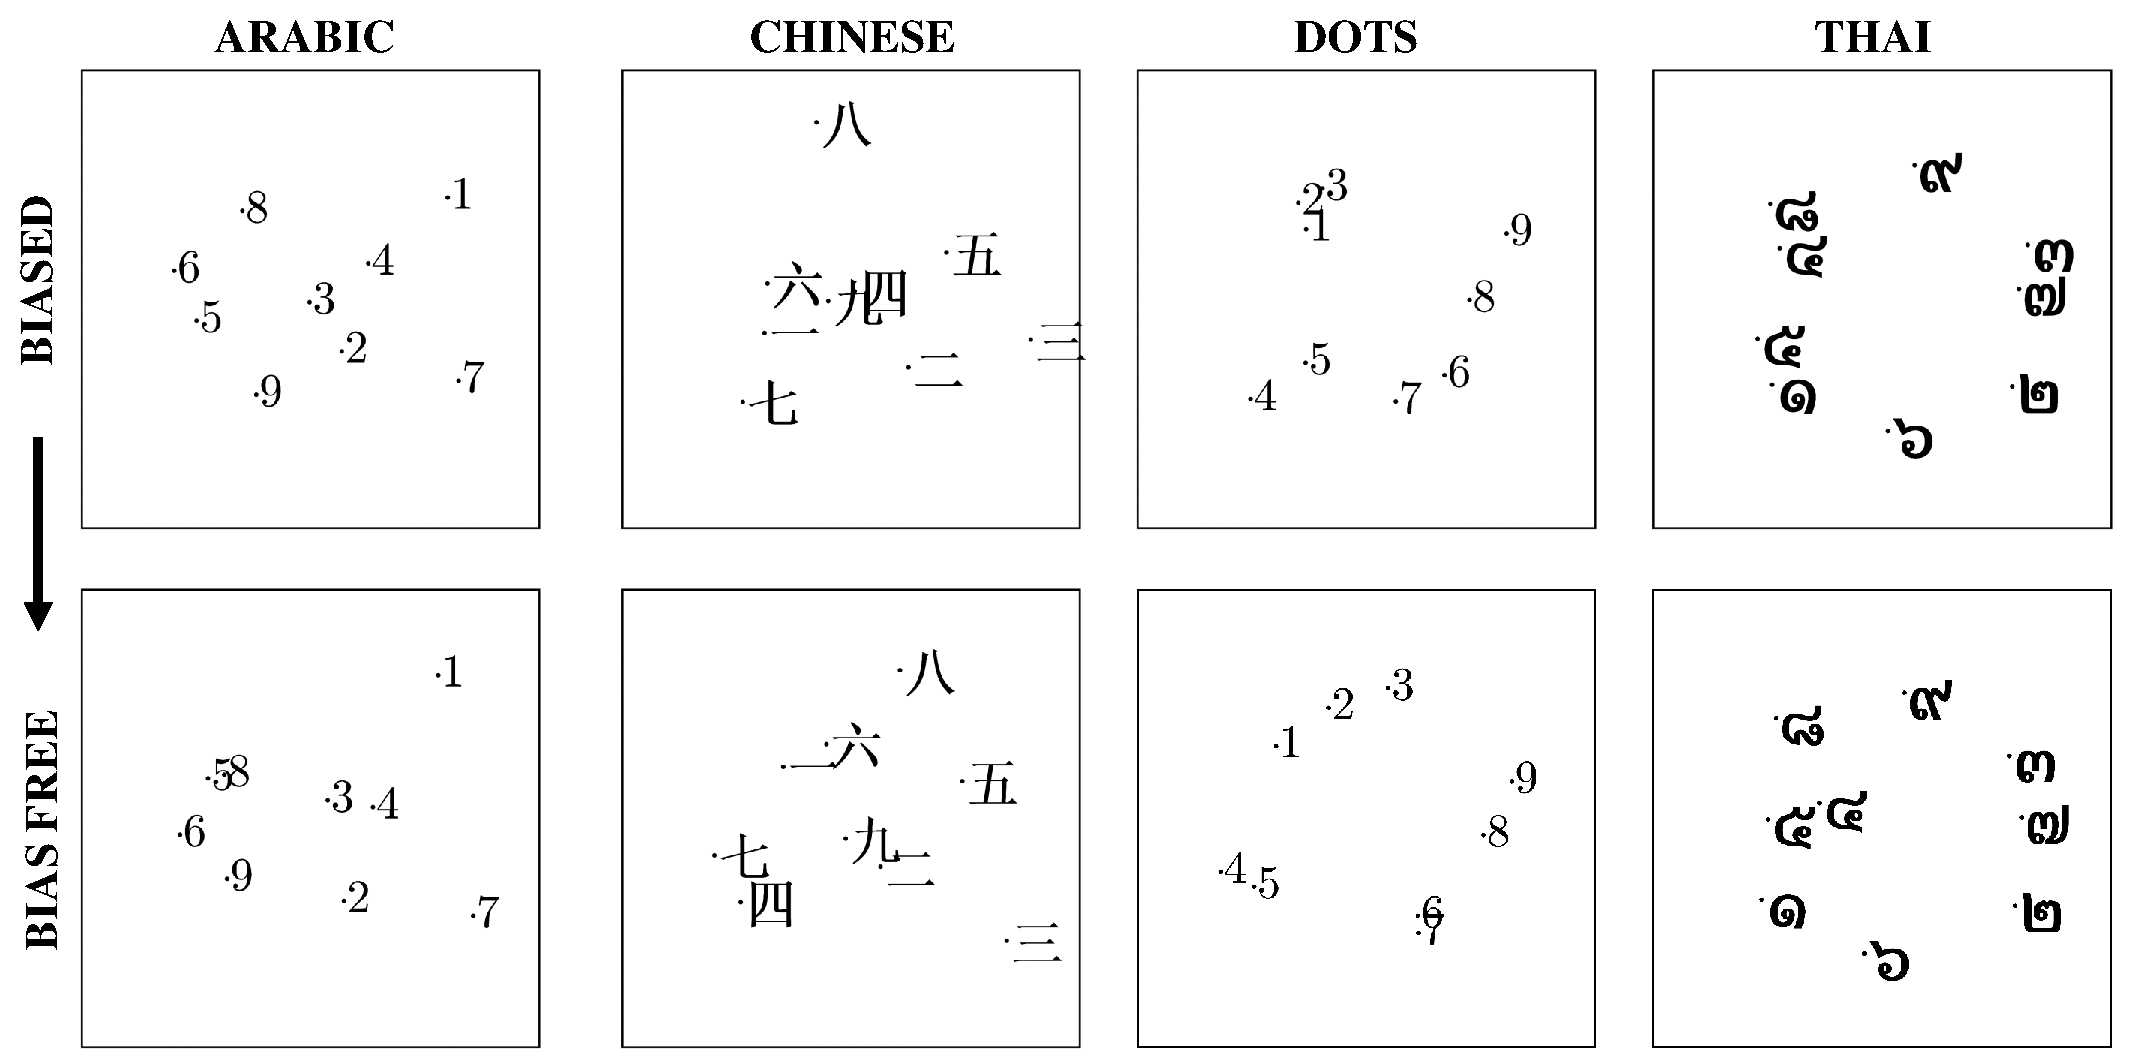
\includegraphics[width = \linewidth]{Figures/CrossWheel/Bias2BiasFree.pdf}
\caption{Biased (uncorrected) and bias free (Luce's choice model corrected) MDS solutions for participant S3, displayed separately for each numeric-type. Changes in item-proximity between biased and bias-free MDS plots display the effect of response-bias on the MDS solution. \\\textbf{Note.} Dots are presented as Arabic numerals to avoid misinterpretation due to spatial overlap.}
\label{fig:Bias2Biasfree}
\end{figure}

\subsection{MDS}
Scree analysis identified two-dimensions as the best MDS representation for most participants in each numeric-type (see supplementary material S5, Figure \ref{fig:Apx_ScreeEngDot_Cross} and Figure \ref{fig:Apx_ScreeChnThi_Cross}). Scree analysis identified three-dimensions as the appropriate MDS representation for one participant in the non-symbolic dots numeric-type, two participants in the Chinese numeric-type, and three participants for the Thai numeric-type. Individual bias-free MDS plots are displayed in supplementary material S5, Figure \ref{fig:Apx_MDSenglish_Cross} -- Figure \ref{fig:Apx_MDSthai_Cross}, and uncorrected MDS plots are displayed in supplementary material S5, Figure \ref{fig:Apx_MDSenglishBiased_Cross} -- Figure \ref{fig:Apx_MDSthaiBiased_Cross}. To describe trends observed across participants, we conducted an Individual Differences Scaling (indscal) MDS analysis. For efficiency of exposition, and as only a select few participants displayed three-dimensional MDS solutions, the following results will focus on the two-dimensional group indscal results.

\subsection{Indscal results}
Figure \ref{fig:Indscal_Cross} (left) displays the two dimensional group indscal MDS solutions for each numeric type. Interpretation of MDS plots is at times arbitrary and relies on visual inspection of the plots. Similarly, interpretation of the MDS solution's axes are also arbitrary with reference to the x- or y-axes \cite<see e.g.,>{nosofsky1986attention, nosofsky2018toward}. Likewise, the notion of similarity is very broad and has been the centre of many disputes in the literature \cite<e.g.,>{tversky1977features, medin1993respects}. To simplify this process, the apparent MDS dimensions have been labelled with directional arrows for each plot. Determining which items cluster together, and the strength of their association in the MDS space is a difficult task. We have formalized this process with an analysis of K-mean clustering. 

\begin{figure}[tbh]
\centering 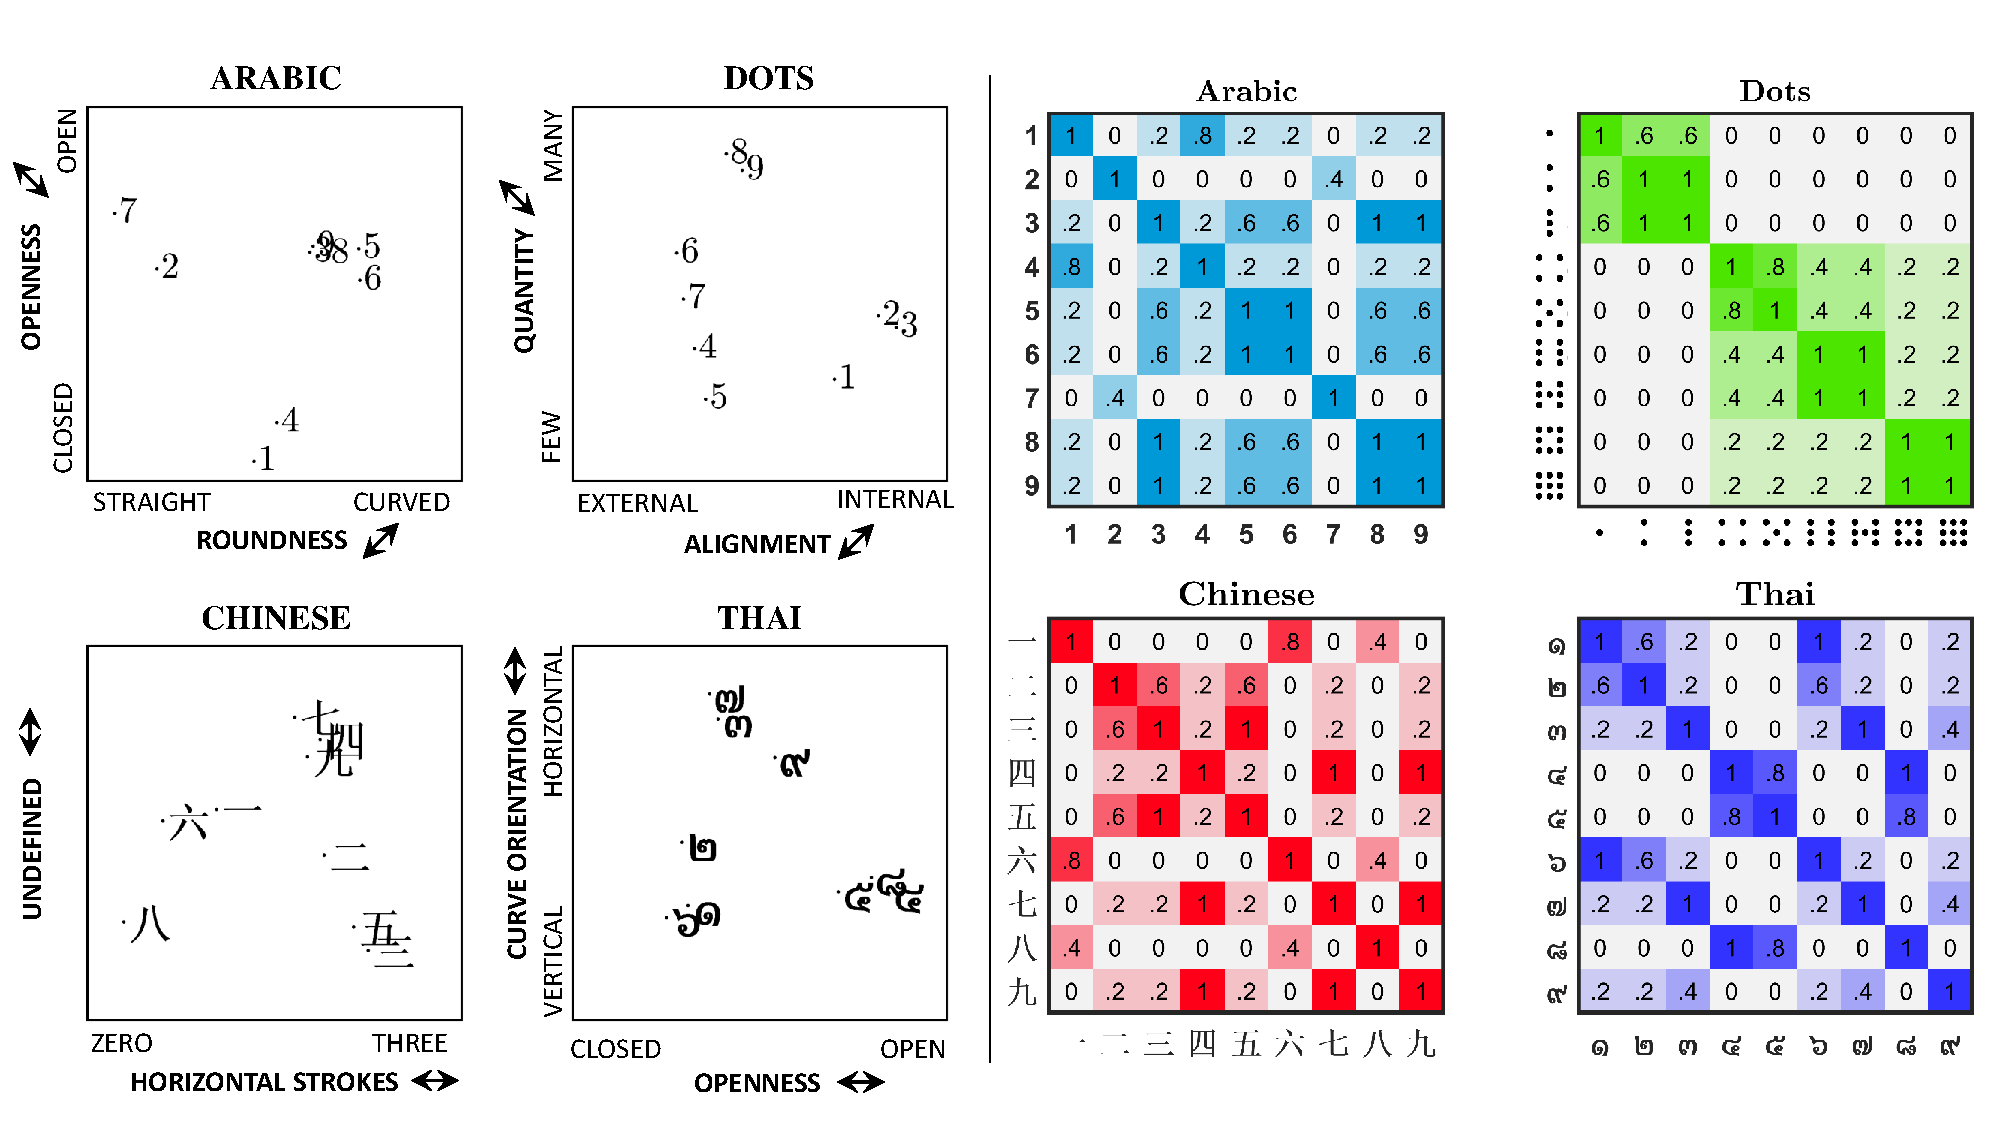
\includegraphics[width = \linewidth]{Figures/CrossWheel/Indscal2D.pdf}
\caption{Left: Individual differences scaling (indscal) solution for all participants best represented by a two-dimensional MDS space, displayed separately for each language-type. Dimensional labels and directionality (arrows) are displayed on the y-axis and x-axis. Right: Proportional cluster-frequency heatmap for MDS indscal results, across 2--6 K-mean clusters. Larger proportions (darker colors) indicate items which cluster most frequently.}
\label{fig:Indscal_Cross}
\end{figure}

Figure \ref{fig:Indscal_Cross} (right) displays an MDS cluster frequency heatmap. For each MDS solution, a K-mean cluster analysis was performed using 2--6 clusters. The proportion at which any two items clustered was calculated for each iteration of K. Where two items clustered on every iteration of K, (\eg Arabic numerals 3 and 8), the proportional frequency was 1. Conversely, where two items never clustered, (\eg Arabic numerals 1 and 2), the proportional frequency was 0. The combination of these methods provides i) a description of the MDS dimensions, and ii) a measure of item similarity strength. This technique provides quantifiable conclusions about item clusters, rather than subjective interpretations. 

Arabic numerals appeared to be represented along two perceptual dimensions of similarity: openness and roundness \cite<similar results were observed by>{godwin2014numSim}. Openness describes the concave absence within a numeral, and roundness describes the curvature of a numeral. Cluster frequency analysis shows strong item-clusters between [3, 8, 9], [1, 4] and [5, 6]. These items all share similar degrees of roundness. Although items [2, 7] grouped within the MDS space, these items did not show a high cluster strength relative to the other groups. The location and proximity of Arabic numerals within the MDS space display no effect of numerical proximity. 

Non-symbolic dots appeared to be represented along the perceptual dimension of alignment, and the numeric dimension of quantity. Alignment describes the positions of dots within the 3 x 3 stimulus array: items 1--3 are centrally aligned, 4--7 are externally aligned, and items 8--9 are both internally and externally aligned. Quantity describes the number of items within the stimulus array. Item clusters present as staggered item-sets, with strong clusters between items [2, 3], [4, 5], [6, 7] and [8, 9]. Item 1 clustered most frequently with items [2, 3], but did not display the same level of cluster strength as the other groups. 



Chinese numerals appeared to be represented along one perceptual dimension that counted the number of horizontal strokes, and a second undefined perceptual dimension. This undefined dimension appears perceptual in origin and displays no apparent influence of numerical proximity. It is possible this dimension is a mixture of different mental representations and therefore cannot be classified at the group level. Individual MDS analyses suggest this could be the case (see supplementary material S5, Figure \ref{fig:Apx_MDSchinese_Cross}). Alternatively, this dimension might reflect a holistic visual process that integrates a range of different perceptual features and cannot be captured by the current scaling method. Item-clusters were strong for numerals \begin{CJK}{UTF8}{gbsn}[四, 七, 九]\end{CJK}, and for numerals that shared similar horizontal stroke counts, for example, \begin{CJK}{UTF8}{gbsn}[一, 六] and [三, 五]\end{CJK}.

Thai numerals appeared to be represented along perceptual dimensions of openness and curve orientation. Curve orientation describes whether Thai numerals had a vertically or horizontally aligned curved feature. Openness describes the concave absence within a numeral. Strong clusters were present between items numbers [1, 6], [3, 7] and [4, 5, 8]. These items all shared features of both openness, and curve orientation. Item number 2 was moderately clustered with items [1, 6], and item number 9 remained independent. 

\subsection{Ideal observer}
The current MDS analysis has made several interpretations based upon dimensions of perceptual similarity. The interpretation of MDS dimensions is a subjective process that may be made stronger by comparing results with an objective benchmark. To this end, we compared the current results to that of the previously conducted ideal observer analysis (Chapter 6). A summary of these results are reported here. A full breakdown is reported in supplementary material S5\ref{Appendix:IOA}. 

MDS and cluster frequency results from the ideal observer displayed very few similarities to our empirical findings. The ideal observer failed to capture the intangible dimension of `openness' and differed greatly from the Arabic and Thai numeral MDS results. Similarly, Chinese numeral MDS results differed greatly between the ideal observer and empirical findings. Finally, ideal observer results were very different for non-symbolic dots, however, as empirical results displayed a combined effect of perceptual similarity and numerical proximity, this finding is to be expected. Together, these results suggest the perceptual dimensions observed in the empirical data go beyond that of simple low level perceptual similarities and reflect higher level dimensions of perceptual similarity, (e.g., openness).

\section{Interim discussion}
Accuracy was successfully manipulated through our staircase procedure. The resulting confusion patterns were subject to Luce's choice model and confusion scores were corrected for the confound of response bias. In line with our hypotheses, MDS indscal and cluster frequency analyses showed that symbolic numerals (Arabic, Chinese, and Thai) appeared to be confused along dimensions of perceptual similarity in the mental space. As predicted, non-symbolic dots appeared to be confused along dimensions of numerical proximity and perceptual similarity in the mental space.

In keeping with our expectations, symbolic numerals appeared to be represented by perceptual dimensions of similarity in the mental space. Familiarity with the Arabic and Chinese numeral sets did not promote an effect of numerical proximity, (i.e., numerical distance). Thai numerals were unfamiliar to the current cohort and as expected, were only confused by dimensions of perceptual similarity. 

In keeping with our previous investigation \cite{garrettWheelTask}, non-symbolic dots appeared to be represented by dimensions of perceptual similarity and numerical proximity within the mental space. There was a clear numerical distance effect --- numerically closer items were confused more often than items further apart. However, this effect was confounded by perceptual similarity and produced staggered item clusters. For example, items [2, 3] and [4, 5] always clustered together, but never items [3, 4] or [5, 6]. Staggered item-clusters only varied by the presence or absence of a single central dot. This means an alternative account of the data could be that numerical proximity confounded the effect of perceptual similarity, producing staggered item-clusters. The co-variation between quantity and perceptual features makes it impossible to disentangle the effects of these dimensions in the mental space using the current results. For now, we may only conclude that dot numerals were confused along dimensions of quantity and alignment, supporting a combined effect of numerical proximity and perceptual similarity on the mental space.

Although the results of the current study aligned with our hypotheses, there are compelling reasons to believe the mental representation of numerals, specifically how numerals are perceived, might change with expertise. For example, the current study employed a Chinese speaking cohort who were familiar with Chinese numerals. This familiarity might alter the perception of Chinese numerals, relative to an inexperienced or naive cohort \cite<e.g.,>{yeh2003role}. To this end, we now compare the results of the current study to the results of the English speaking cohort as presented in the previous Chapter. 


\section{Cohort comparison results}
\subsection{Accuracy}
Mean accuracy was comparable between cohorts for each numeric-type, and error rates were sufficient for MDS analysis. On average, the Chinese speaking cohort was more accurate ($\mu$ = .65, $\sigma$ = .12) than the English-speaking cohort ($\mu$ = .58, $\sigma$ = .14), a trend that held within each numeric-type. On average, the English speaking cohort was most accurate for non-symbolic dots ($\mu$ = .65, $\sigma$ = .12), Thai numerals ($\mu$ = .64, $\sigma$ = .1), Chinese numerals ($\mu$ = .61, $\sigma$ = .15), and finally Arabic numerals ($\mu$ = .55, $\sigma$ = .15). A direct comparison of accuracy between cohorts is difficult due to the differences between testing facilities. Each testing facility employed different monitors (CRT vs LCD) and ambient lighting. This produced similar levels of accuracy between the two cohorts, at different signal contrast levels.


Figure \ref{fig:ComparedAccuracy} displays the matched signal-contrast accuracy for the Chinese speaking cohort (left) and the English speaking cohort (right). Participants viewed stimuli at five levels of signal contrast and the average accuracy for each of these signal-levels is plotted Figure \ref{fig:ComparedAccuracy}. For example, if for Arabic numerals, participant S1 viewed stimuli at RGB values 134--137, and participant S2 viewed stimuli at RGB values 137--141, their accuracy at the shared contrast value of 137 would be averaged and plotted in the figure. By matching accuracy across contrast-levels, we may compare accuracy trends for each numeric-type within each cohort. This method also allows us to compare accuracy trends between cohorts by comparing the relative ordering of the numeric-types. Differences between the actual contrast levels reflect perceptual differences incurred at each testing facility.

\begin{figure}[tbh]
\centering \includegraphics[width=\linewidth]{Figures/CrossWheel/Comparison_AccuracySubplot.jpg}
\caption{Mean accuracy matched by contrast-level for the Chinese speaking cohort (left) and English speaking cohort (right) across numeric types. Note, only RGB values with multiple data points are displayed. Error bars represent one standard-error of the mean.}
\label{fig:ComparedAccuracy}
\end{figure}

When accuracy was matched by signal contrast level, unfamiliar Thai numerals displayed the lowest accuracy trends across both cohorts. Within the Chinese speaking cohort, non-symbolic dots displayed the highest level of accuracy at lower contrast levels, and crossed over with Arabic and Chinese numeral accuracy trends at higher contrast levels. Arabic and Chinese numerals displayed comparable accuracy across the range of contrast levels. Within the English speaking cohort, non-symbolic dots and Arabic numerals displayed similar trends in accuracy across the range of contrast levels, and were slightly more accurate than Chinese numerals. These results display a trend whereby familiar numerals within each cohort were responded to with greater accuracy than unfamiliar numerals, given the same level of signal contrast. 

\subsection{Confusion scores}
Confusion scores, the rate at which one numeral is erroneously confused with another, index proximity between items in the mental space. If confusions are strongly correlated between cohorts, similar representations may exist between the mental spaces of each cohort. We calculated the Pearson's correlation ($r$) between cohort confusion scores for each numeric type, after setting the main diagonal (accurate identifications) to zero. This was done for the uncorrected (biased) confusion scores, and the bias-free confusion scores. 

Uncorrected confusion scores, (i.e., confusions scores before the application of Luce's choice model) were highly correlated for Arabic ($r$ = .9, $p <$ .001), non-symbolic dot ($r$ = .9, $p <$ .001), Thai ($r$ = .89, $p <$ .001) and Chinese numerals ($r$ = .87, $p <$ .001). These correlations increased with the removal of response-bias for Arabic ($r$ = .94, $p <$ .001), non-symbolic dot ($r$ = .97, $p <$ .001), Chinese ($r$ = .92, $p <$ .001), and Thai numerals ($r$ = .95, $p <$ .001). The correlation of bias free confusion scores suggests that, between cohorts, the mental space is most similar for non-symbolic dots, than Thai numerals, Arabic numerals and finally, Chinese numerals. Further examination of the similarities and differences between the mental representations of each cohort requires MDS comparisons.

\subsection{MDS comparison}
Figure \ref{fig:IndscalCompared_Procrustes} displays the group MDS indscal solutions for the Chinese-speaking cohort (left column) and English-speaking cohort (middle column). The apparent dimensions along which numerals were represented in the mental space are displayed along the x- and y-axes. Similar dimensions were observed between cohorts for Arabic numerals (openness vs roundness), non-symbolic dots (quantity vs alignment) and Thai numerals (curve orientation vs openness). Chinese numerals were represented along different dimensions in the Chinese-speaking cohort (an undefined perceptual dimension vs the number of horizontal strokes) and English-speaking cohort (the number of line terminations vs the stroke alignment; see Figure \ref{fig:IndscalCompared_Procrustes}). To empirically assess the degree of similarity between these MDS representations, we performed a procrustes analysis on the group indscal results.

\newpage
\begin{figure}[!htb]
\centering \includegraphics[width=\linewidth]{Figures/CrossWheel/IndscalCompared.pdf}
\caption{Indscal MDS solutions for the Chinese speaking cohort (left), English speaking cohort (middle) and a procrustes analysis fitting the English cohort to the Chinese cohort's MDS solutions (right). Colored items represent the English cohort's transformed MDS indscal solution fit to the Chinese MDS indscal solution. Standardised sum of squared errors (goodness of fit) is reported in the top left of each panel; a lower SS$_{error}$ indicates a better fit between cohorts.}
\label{fig:IndscalCompared_Procrustes}
\end{figure}

The procrustes analysis fits one MDS representation to another through a combination of translation (moving one over the other), rotation and scaling. A measure of fit is provided by the standardized sum of squares error. This affords a direct comparison of `goodness of fit' between numeric-types, with an SS$_{error}$ closer to zero indicating a better procrustes fit. The right column of Figure \ref{fig:IndscalCompared_Procrustes} displays the procrustes results, fitting the English-speaking cohort's MDS results (colored numerals) to the Chinese-speaking cohort's MDS results (black numerals). In line with the correlational analyses, MDS representations were most similar for non-symbolic dots (SS$_{error}$ = .05), then Thai numerals (SS$_{error}$ = .035) and Arabic numerals (SS$_{error}$ = .192). MDS results were most dissimilar for Chinese numerals (SS$_{error}$ = .729).

\section{General discussion}
When asked to identify Arabic, Chinese, Thai and dot numerals, both Chinese-speaking and English-speaking cohorts where able to complete the tasks with similar levels of accuracy. In both cohorts, familiar numeric sets were more accurately responded to than unfamiliar numeric sets, after controlling for signal-contrast. Correlational and procrustes analyses showed MDS representations were similar between cohorts for Arabic numerals, non-symbolic dots and Thai numerals. MDS representations differed between cohorts for Chinese numerals --- the only numeral set where cohorts also differed in their levels of expertise. For both cohorts, Chinese numerals appeared to be represented along dimensions of perceptual similarity, however, the perceptual features confused by each cohort differed greatly. Chinese speakers appeared to confused Chinese numerals by the number of horizontal strokes and by an undefined dimension of perceptual similarity. English  speakers appeared to confused Chinese numerals along the dimensions of character alignment and the number of line terminations. Both cohorts appeared to confuse Chinese numerals by low-level dimensions of perceptual similarity, and Chinese speakers did not show evidence of global or holistic processing relative to the English speaking cohort. 

\subsection{Expertise and the mental space}
The mental representations of Chinese numerals varied greatly between the Chinese and English speaking cohorts. Against predictions, the mental representations of Chinese speakers did not show signs of global or holistic processing. In line with predictions, the mental representations of English speakers displayed evidence of localised visual processing. Both cohorts appeared to represent Chinese numerals along dimensions of perceptual similarity, however, only the English speaking cohort were influenced by the logographic nature of the numeric set.

Chinese characters are logographic such that each character holds a unique semantic meaning. Chinese numerals are a special among these logographs, with many numerals physically symbolizing their value. For example, the Chinese characters \begin{CJK}{UTF8}{gbsn} 一, 二, 三, 四 \end{CJK} are the numerals 1--4 as indicated by the sum of their outer lines. By happenstance, Chinese numerals less-than five and greater-than five are made from predominantly horizontal and vertical line strokes, respectively. Together, these perceptual and logographic elements clearly demarcate small and large values within the range of 1--9. These influences are clearly visible within the English speaking cohort, however, are absent from the Chinese speaking cohort. 

Chinese speakers did not represent Chinese numerals by stroke alignment or the by logographic elements of the numerals. It appears that, with expertise, Chinese speakers knew to focus upon specific numeric identifiers that were not apparent to the English speaking cohort. For example, Chinese speakers appeared to focus upon the number of horizontal stroke elements. The undefined perceptual dimension within the Chinese speaking cohort might reflect a mixture of these expert visual processes. Unfortunately, this cannot be discerned from the group MDS analysis and is equally unclear at the individual level. Future investigations using our methodology might consider asking participants to describe their visual processing strategy. This may help in classifying individuals with similar MDS representations.

The results of the current study clearly show that expertise with a numeric set may change the way we perceive and represent items within the mental space. Our work adds to the established literature that examines how cognitive processes evolve with training and expertise \cite{yeh2003role, gauthier2003perceptual, chua2019domain}. Our work also shows how our mental representations can be stable across cultures given similar levels of expertise. 

\subsection{Similarities in the mental space}
The mental representations of non-symbolic dots, Thai and Arabic numerals were very similar across cohorts. Arabic and dot numerals were very familiar to both cohorts, and Thai numerals were unfamiliar to both cohorts. These similarities show that, with similar levels of expertise, stable mental representations are formed across our two cultures. 

Non-symbolic dots were most similarly represented across cohorts. This was not unexpected. Dots are a physical representation of quantity and activate the innate ANS. This numeric set validates our experimental methods and analysis techniques, producing nearly identical mental representations across both cohorts.

The mental representations for Thai numerals were the next most similar. Being unfamiliar to both cohorts, these results reflect the similar visual processes employed by both cohorts. In a future study, it would be interesting to assess the mental representation of these numeric stimuli within a Thai speaking cohort. For now, whether these stimuli are processed differently after acquiring expertise remains an unanswered question.

Arabic numerals were similarly represent across cohorts, however, to a lesser extent than Thai and non-symbolic dots. Similar mental representations were expected between cohorts, as both share similar level of expertise. However, Arabic numerals form part of a secondary language for the Chinese speaking cohort, and a primary language for the English speaking cohort. Therefore, it is possible that a small difference in expertise exists between the cohorts. This difference might explain why Arabic numerals are most different in their representations from among the non-symbolic dot, Thai and Arabic numeric types. It is fortunate and commendable that our methods and analysis techniques were able to capture this nuanced difference. 


\subsection{Future research}
The current research has shown that expertise changes the way Chinese numerals are represented within the mental space. However, the results of this study differed from our expectations \cite{yeh2003role} and may reflect a difference in methodology. We propose a future study using the spatial arrangement method \cite<as used by>{yeh2003role} in an English speaking and a Chinese speaking cohort. Using the numeric sets of the current study, participants could be asked to arrange items by perceptual similarity, and separately, by numerical proximity. Such an investigation could disentangle perceptual and semantic effects in the mental space, and determine whether the differences between the current study and \citeauthor{yeh2003role}'s investigation are due to task design. 


\subsection{Implications}
The clear communication of numeric value is important in many tasks, including finance, teaching, timekeeping and transportation. Much time can be spent crafting or selecting numeric fonts that enhance this communication. For example, it is important to have clear numeric fonts for vehicular speed signs, especially when road conditions are not ideal. The current research and methodology can be easily extended to the assessment of fonts, either within a culture, (\eg Taiwanese drivers in Taiwan), or across cultures, (\eg Australian drivers visiting Taiwan), with the aim of enhancing public safety and written communication. 

The current methodology has proven effective at examining latent cognitive dimensions (numeric proximity) between two cultures. The methods of this study could be equally applied to examine other latent dimensions, for example alphabetic proximity \cite<as shown by>{townsend1971alphabetic}, and how these latent dimensions change with expertise or due to differences between cultures. 

\section{Conclusion}
The ability to accurately communicate quantity through symbolic numerals plays an important role in all human cultures. Often, as we navigate our busy and dynamic environments, we confused the identify of one numeral for another. Such confusions provide insight into how these numeric symbols are represented within our mental space. Although past research has examined the mental dimensions of numeric item-sets, these assessments were confounded by participant response bias. We have presented bias free mental representations of familiar and unfamiliar numeric-sets in both Chinese-speaking and English-speaking cohorts. We have shown how expertise with a language-set may change the representation of numerals within the mental-space. We have also shown clear similarities in the mental representations of two different cohorts, for familiar (Arabic and dot) and unfamiliar (Thai) numerals. While expertise with a numeric set may change our mental landscape, we show that when items are novel (unfamiliar) or universally understood across cultures (symbolic dots), our mental representations are essentially the same. 

% AMI DONE 1/11/2019

\chapter{General conclusions} 

\label{Chapter 8}

\lhead{Chapter 8. \emph{General conclusions}}

This thesis offers a number of contributions to the literature on numerical cognition. In the first research stream, the comparison of quantities (Chapters 2--5), I examined the cognitive processes with which we estimate a single item-set (Chapter 2) and applied these findings to study the processing architecture and workload capacity of a comparative estimation system (Chapter 3). This work led to a subsequent investigation examining the systems of comparative subitizing (Chapter 4). In these studies, I applied Systems Factorial Technology to analyse response times and uncover basic properties of the underlying processing system. I observed empirical SIC signatures that indicated a mixture of two different processing architectures. To identify these mixtures, I completed a simulation study that extended the canonical SIC signatures to systematic mixtures of processing architecture and workload capacity (Chapter 5). In the second research stream, the confusion of numbers (Chapters 6 \& 7), I examined the mental representations of familiar and unfamiliar numerals within an English (Chapter 6) and Chinese (Chapter 7) speaking cohorts. Across both cohorts, I found that symbolic numerals were represented along dimensions of perceptual similarity, and non-symbolic numerals along dimensions of perceptual similarity and numerical proximity. Finally, I found that expertise may change the way we perceive numerals and thereby shape our mental representations. 
%AE: fine, but you know i think these conclusions are not grounded
%PG: I know, but I'm going with it :p We'll just need to see what the reviewers think

Each of the above thesis chapters have worked in concert to extend our understanding of numerical cognition. Together, these chapters formed two complimentary research streams: one that investigated the enumeration of non-symbolic quantities, and one that investigated the representation of symbolic numerals. Although I have discussed these streams as independent components, a complete understanding of numerical cognition requires the simultaneous investigation of both symbolic and non-symbolic quantities.
% AE: I edited last para' so check that you agree
% PG: Great, thanks Ami

Numerical cognition encompasses the communication of quantity through coarse non-symbolic values, for example, tallies and dots, and the precise communication of symbolic digits. Numerical cognition describes our mental representations of number and quantity, and how these constructs are informed by our past experiences and current levels of expertise. Finally, numerical cognition is the complimentary understanding of both quantities \textit{and} numbers, as epitomized by my complimentary research streams. Together, these two research streams aimed to extend our scientific understanding of numerical cognition through the examination of both quantities and numbers.

%AE: do you mean complementary ? 
% PG: Yes, thanks for that!
The research chapters and complementary research streams of this thesis have made several substantial contributions to the literature. The research chapters of this thesis have extended on previous methodological designs (Chapters 2, 3, 4, and 6), developed new analysis techniques (Chapters 5 and 6), and provided new insights on the fundamental cognitive processes that we share across cultures (Chapter 7). In each of these chapters, I have discussed these contributions in detail. Rather than retread these points, I will now discuss the general implications and the future directions that stem from this thesis. 

%AE: i substituted research component with 'research strand'; for consistency perhaps do this in ALL of the thesis?
%PG: I've gone with stream - same use, I just like it more than strand.

\section{Implications and future directions}
\subsection{Systems of enumeration}
The work reported in the current thesis has many implications for the field of numerical cognition. In the first research stream, I considered systems of estimation and subitizing. I observed that estimation systems operate under predominantly parallel processing architectures, and that subitizing systems operate under predominantly serial processing architectures. In both instances, these systems were less-efficient than the predictions of a theoretical serial processing system. I suggested that this was due to context effects. This work is important, not only for the design of future research, but for the interpretation of past findings. 

Studies that investigate processes of enumeration often display an array containing two or more item sub-sets \cite<e.g., green, red and blue colored discs;>{HALBERDA_2006}. These studies generally work under the implied assumption of context invariance --- that the cognitive process operating on one item-set is unaffected by the presence of another. Our work clearly violates this assumption for both small and large quantities. This means that past and future research that relies on the interpretation of response-times, must consider the inhibitory influence of these context effects within the domain of enumeration. Future research can examine what these context effects are, and how they can be ameliorated.

\subsection{Systems factorial technology}
Systems factorial technology and the associated measure the SIC($t$), has been used by Townsend and colleagues \cite{Townsend_1995, Townsend_2004, eidels2010stroop, Fific2010, houpt2010statSIC, Little2011, Little2017} to diagnose processing architecture in a range of experimental tasks. Typically, the SIC is compared to canonical signatures and is used to diagnose processing architecture (parallel vs serial) and stopping-rule (minimum-time vs maximum-time). In Chapter 5, I developed a class of mixture models and reported new SIC signatures, corresponding to systematic mixtures of processing architecture. 

Our new mixture SIC($t$) signatures have implications for both past and future work. Previously, SIC($t$) signatures that did not match  a single canonical model were either i) not diagnosed, ii) diagnosed by the best matching canonical model, or more recently iii) fit parametrically as a mixture or contaminant model \cite{Moneer2016}. By providing a new set of signatures for mixture models, SIC(\textit{t}) functions can be diagnosed by their component architectures and relative proportions. Future research will need to consider non-parametric statistical methods through which these mixture models may be diagnosed. This would add to the growing suite of statistical tools \cite<\eg>{houpt2010statSIC, houpt2012statCap, houpt2017bayesSIC, houpt2017hierarchical, Moneer2016} used by the SFT community for diagnosing system properties. This work might also extend to diagnosing mixtures of stopping-rule \cite{TillmanStopping}. 

\subsection{Numeral identification}
In the second research stream, the confusion of numbers, I investigated the mental representation of numerals across English and Chinese speakers. Across these two cohorts, I found that mental representations changed in response to different levels of numeric expertise. Importantly, when numeric expertise was the same between cohorts, mental representations were nearly identical. This work presents new questions and potential lines of inquiry regarding the effect of expertise on our mental representations. 

Future research could examine how experience alters the proximity of items within the mental space. For example, does the frequency of exposure to unfamiliar numerals shift items in the mental space? Or, does a shift in the mental space require unfamiliar numerals to be processed at a deeper cognitive level, for example, by using them for arithmetic operations? Furthermore, what are the temporal constraints to these processes. For example, how long do changes to the mental space take, and do these changes affect different dimensions at different rates? These questions could be applied to any investigation of expertise using confusion patterns, however, as we have shown, numerals appear to be particularly well suited to this task. 

In a second line of future research, I propose a final extension of the work in Chapter 6 and 7 by examining the mental representation of numerals within a Thai cohort. In both of the tested cohorts, Thai numerals served as a symbolic control, with neither cohort having any experience with the numeric set. Replicating our investigation with a Thai cohort would give deeper insight into i) whether Thai numerals shift in the mental space with experience, and ii) further validate that non-symbolic numerals are represented identically across cultures. If this cohort had little expertise with Arabic numerals, this investigation might address iii) whether similarities between Australian and Taiwanese representations for Arabic numerals reflected numeric expertise. 

Finally, my work on confusion analysis not only represents an important contribution to numerical cognition, but a contribution to methodological design. In this work, I developed a rapid staircase procedure, applied a method for removing response-bias, modelled group level MDS data and examined MDS distances through an objective clustering technique. The combination of these experimental and analytic methods produced clear, illustrative results that were easy to compare within and between our cohorts. Importantly, these principled methods can be applied in any investigation of confusion data. 


\section{Conclusion}
The ability to compare quantities and symbolic numerals has shaped the course of human history. Every aspect of human culture, from trade and science, to mathematics and war, has been advanced by our understanding of quantities and numbers. In the modern era, we regularly compare two quantities, (\eg number of people in coffee queues), and communicate symbolic value, (\eg phone numbers and money). Until recently, the cognitive processes that underpin such abilities have been poorly understood. The aim of this thesis was to provide new insights into the fundamental cognitive processes that govern our comparisons of quantity and our confusion of numbers. Over the course of the past seven chapters, I addressed this aim by developing theoretically driven experimental designs, analyses and simulations.In accordance with the aim of this thesis, I have shed new light on the nature of the cognitive processes that are fundamental to our understanding of quantity and number. Yet, so much more remains to be learned. Future researchers have much to explore on the nature of numerical cognition. I am sure the findings of these studies will be both enlightening and numerous.

%AMI DONE 1/11/2019



\clearpage
%\addcontentsline{toc}{section}{Online Supplementary Materials}
%\addtocontents{toc}{\vspace{2em}}

\backmatter % i, ii, iii

\clearpage
\lhead{References}
\bibliographystyle{apacite}
\renewcommand\bibname{References}
\bibliography{references}
\clearpage


\addtocontents{toc}{\vspace{3em}}
\appendix
\renewcommand{\appendixname}{Supplementary Material}

\chapter{Online Supplementary Materials}
You can download the \href{https://github.com/paulgarrettphd/Site/raw/master/thesis/SupplementaryMaterials_PaulGarrett_Thesis_2019.pdf}{\color{blue}Supplementary Materials here\color{black}} or find them on my GitHub located under the repository paulgarrettphd/Site/thesis. You can also contact me directly at Paul.Garrett2016@gmail.com.

\lhead{Supplementary Materials}
\chapter{Supplementary Materials S1: \\ Estimation Systems}
\label{Appendix:A_EstimationSystems}
\lhead{Supplementary S1. \emph{Estimation Systems}}

\noindent The materials in this supplementary chapter are relevant to Chapter 3 of the submitted thesis.

%\renewcommand{\thepage}{s.\arabic{page}}
\setcounter{page}{1}
\setcounter{equation}{0}
\setcounter{figure}{0}
\setcounter{table}{0}
\setcounter{section}{0}
\renewcommand\thefigure{S1\thesection.\arabic{figure}}
\renewcommand\thetable{S1\thesection.\arabic{table}}

\newpage

\section{Estimation system workload capacity}
\label{Appendix:A_EstWorkload}

\subsection{Experiment 1: Fixed Item-Size, Mixed Item-Sets}
\begin{figure}[htb]
\begin{center}
\includegraphics[width=\linewidth]{Figures/Appendix/FIG16JPG.jpg}
\caption{Capacity coefficient plots for each individual subject in Experiment 1. Dotted line depicts the Grice lower-bound. Black solid line illustrates the target capacity coefficient. All capacity coefficients are illustrated as on or below the lower-bound, suggesting severe workload capacity limitations in all subjects.}
\label{fig:Indiv_Cap_Ex1}
\end{center}
\end{figure}

\newpage
\subsection{Experiment 2: Fixed Item-Size, Spatially Separate Item-Sets}
\begin{figure}[htb]
\begin{center}
\includegraphics[width=\linewidth]{Figures/Appendix/FIG17JPG.jpg}
\caption{Capacity coefficient plots for each individual subject in Experiment 2. Dotted line depicts the Grice lower-bound. Black solid line illustrates the target capacity coefficient. All capacity coefficients are illustrated as on or below the lower-bound, suggesting severe workload capacity limitations in all subjects.}
\label{fig:Indiv_Cap_Ex2}
\end{center}
\end{figure}

\newpage
\subsection{Experiment 3: Fixed Item-Set Area, Mixed Item-Sets}
\begin{figure}[htb]
\begin{center}
\includegraphics[width=\linewidth]{Figures/Appendix/FIG18JPG.jpg}
\caption{Capacity coefficient plots for each individual subject in Experiment 3. Dotted line depicts the Grice lower-bound. Black solid line illustrates the target capacity coefficient. All capacity coefficients are illustrated as on or below the lower-bound, suggesting severe workload capacity limitations in all subjects.}
\label{fig:Indiv_Cap_Ex3}
\end{center}
\end{figure}

\newpage
\subsection{Experiment 4: Fixed Item-Set Area, Spatially Separated Item-Sets}
\begin{figure}[htb]
\begin{center}
\includegraphics[width=\linewidth]{Figures/Appendix/FIG19JPG.jpg}
\caption{Capacity coefficient plots for each individual subject in Experiment 4. Dotted line depicts the Grice lower-bound. Black solid line illustrates the target capacity coefficient. All capacity coefficients are illustrated as on or below the lower-bound, suggesting severe workload capacity limitations in all subjects.}
\label{fig:Indiv_Cap_Ex4}
\end{center}
\end{figure}

\newpage
\section{Resilience Difference}
\label{Sup: Rdiff}

\begin{figure}[tbh]
\centering \includegraphics[width=\linewidth]{Figures/Appendix/FIG20JPG.jpeg}
\caption{Resilience difference plots for Estimation Experiments 1 – 4 when target salience is high. Black lines depict the average resilience difference function across subjects, while grey markers illustrate individual subject’s resilience difference functions. Average plots show a trend towards \Rd = 0, supporting predictions made by an unlimited-capacity parallel minimum-time processing system.}
\label{fig:RdiffHigh}
\end{figure}


\newpage
\section{Processing Architecture}
\label{Appendix: DT_Arch}
\subsection{Experiments 2--4}
\begin{table}[htb]
\caption{Table of individual double-target MIC and SIC results from Experiments 2--4. From left to right, ANOVA main effects for red target salience (R) and blue target salience (B), MIC value and interaction significance, Bayesian SIC model probability and associated architecture, and Bayes factor values from the hierarchical MIC analysis with associated processing architecture results: Parallel (P) and Serial (S).}
\centering 
\begin{tabular*}{\textwidth}{l @{\extracolsep{\fill}} lllllll}
\hhline{-------}
\textbf{Sub  } & \textbf{\begin{tabular}[c]{@{}c@{}}Main \\ Effects\end{tabular}} & \textbf{MIC} & \textbf{SIC} $\mathbb{P}$ & \textbf{SIC Model} & \textbf{BF$_{10}$} & \textbf{MIC Model} \\  
\hhline{-------}
202 & R \& B & 30*   &\textbf{0.57}& \textbf{P Min-Time}  & \textbf{4.6}  & \textbf{P Min-Time}\\
205 & R \& B & 112*  & &                                  & \textbf{15.32} & \textbf{P Min-Time}\\
212 & R \& B & 8     &0.44         & P Min-Time           & \textbf{3.18}  & \textbf{P Min-Time}\\
214 & R \& B & 142** &\textbf{0.95}& \textbf{P Min-Time}  & \textbf{18.75} & \textbf{P Min-Time}\\
215 & R \& B & 78* 	 &\textbf{0.67}& \textbf{P Min-Time}  & \textbf{10.42}  & \textbf{P Min-Time}\\
\hhline{~~~~---}
~&~&~&~& \textit{MIC Group Posterior}                              & \textbf{5.11}  & \textbf{P Min-Time} \\       
\hhline{-------}
303 & R \& B & 128** &\textbf{0.95}& \textbf{P Min-Time}  & \textbf{13.95} & \textbf{P Min-Time}\\ 
307 & R \& B & -7    &0.41& P Min-Time                    & 2.27 & P Min-Time\\      
310 & R \& B & 26    &\textbf{0.64}& \textbf{P Min-Time}  & \textbf{3.35} & \textbf{P Min-Time}\\      
311 & R \& B & 13    &&                                   & 2.44 & P Min-Time\\
318 & R \& B & 67* 	 &\textbf{0.69}& \textbf{P Min-Time}  & \textbf{6.9} & \textbf{P Min-Time}\\ 
\hhline{~~~~---}
~&~&~&~& \textit{MIC Group Posterior}                              & \textbf{3.42} & \textbf{P Min-Time} \\ 
\hhline{-------}
402 & R \& B & -45*  &\textbf{0.65}& \textbf{P Max-Time}  & 1.9   & P Max-Time\\     
407 & R \& B & 72**  &\textbf{0.64}& \textbf{P Min-Time}  & \textbf{8.73}  & \textbf{P Min-Time}\\ 
414 & R \& B & 116** &&                                   & \textbf{12.42} & \textbf{P Min-Time}\\         
416 & R \& B & -54*  &\textbf{0.91}& \textbf{P Max-Time}  & 2.68  & P Max-Time\\ 
\hhline{~~~~---}
~&~&~&~& \textit{MIC Group Posterior} & 2.68 & P Min-Time \\
\hhline{-------} \hhline{-------}
\multicolumn{7}{p{\textwidth}}{MIC interaction significance tests were conducted at p $<$ .33*, p $<$ .05** and p $<$ .01***. Conclusive model architectures were based upon an SIC model selection probability $>$ 0.5 and are displayed in bold font. MIC models with moderate evidence (BF$_{10}$ $>$ 3) are also displayed in bold font.}
\end{tabular*} 
\label{table:DT} 
\end{table}

\newpage

\label{Sup: indSIC}
\subsection{Experiment 1: Fixed Item-Size, Mixed Item-Sets Double-Target SIC}
\begin{figure}[htb]
\begin{center}
\includegraphics[width=\linewidth]{Figures/Appendix/FIG23PNG.png}
\caption{Double-Target survivor interaction contrast (SIC) plots for each individual subject in Experiment 1. Dotted line illustrates the bootstrap of the standard error.\newline
\textbf{Note.} MIC interaction contrast significance defined at $p$* $<$ .33, $p$** $<$ .05, $p$*** $<$ .01. D-statistic, a measure of SIC deviance from SIC($t$) = 0 significance defined at $\alpha$ $<$ 0.15.}
\label{fig:Indiv_SIC_AB_Ex1}
\end{center}
\end{figure}
\newpage

\subsection{Experiment 2: Fixed Item-Size, Mixed Item-Sets Double-Target SIC}
\begin{figure}[htb]
\begin{center}
\includegraphics[width=\linewidth]{Figures/Appendix/FIG24PNG.png}
\caption{Double-Target survivor interaction contrast (SIC) plots for each individual subject in Experiment 2. Dotted line illustrates the bootstrap of the standard error.\newline
\textbf{Note.} MIC interaction contrast significance defined at $p$* $<$ .33, $p$** $<$ .05, $p$*** $<$ .01. D-statistic, a measure of SIC deviance from SIC($t$) = 0 significance defined at $\alpha$ $<$ 0.15.}
\label{fig:Indiv_SIC_AB_Ex2}
\end{center}
\end{figure}
\newpage

\subsection{Experiment 3: Fixed Item-Size, Mixed Item-Sets Double-Target SIC}
\begin{figure}[htb]
\begin{center}
\includegraphics[width=\linewidth]{Figures/Appendix/FIG25PNG.png}
\caption{Double-Target survivor interaction contrast (SIC) plots for each individual subject in Experiment 3. Dotted line illustrates the bootstrap of the standard error.\newline
\textbf{Note.} MIC interaction contrast significance defined at $p$* $<$ .33, $p$** $<$ .05, $p$*** $<$ .01. D-statistic, a measure of SIC deviance from SIC($t$) = 0 significance defined at $\alpha$ $<$ 0.15.}
\label{fig:Indiv_SIC_AB_Ex3}
\end{center}
\end{figure}
\newpage

\subsection{Experiment 4: Fixed Item-Size, Mixed Item-Sets Double-Target SIC}
\begin{figure}[htb]
\begin{center}
\includegraphics[width=\linewidth]{Figures/Appendix/FIG26PNG.png}
\caption{Double-Target survivor interaction contrast (SIC) plots for each individual subject in Experiment 4. Dotted line illustrates the bootstrap of the standard error.\newline
\textbf{Note.} MIC interaction contrast significance defined at $p$* $<$ .33, $p$** $<$ .05, $p$*** $<$ .01. D-statistic, a measure of SIC deviance from SIC($t$) = 0 significance defined at $\alpha$ $<$ 0.15.}
\label{fig:Indiv_SIC_AB_Ex4}
\end{center}
\end{figure}
\newpage


\section{Individual MIC Plots}
\label{Sup: IndMIC}


\subsection{Experiment 1: Fixed Item-Size, Mixed Item-Sets Double-Target MIC Plots}
\begin{figure}[htb]
\begin{center}
\includegraphics[width=\linewidth]{Figures/Appendix/FIG27PNG.png}
\caption{Double-Target mean interaction contrast (MIC) plots for each individual subject in Experiment 1. White-eggs indicate blue-target high-salience, black-eggs blue-target low-salience. Error bars are $\pm$1 standard error of the mean.  \newline
\textbf{Note.} MIC interaction contrast significance defined at $p$* $<$ .33, $p$** $<$ .05, $p$*** $<$ .01}
\label{fig:Indiv_MIC_AB_Ex1}
\end{center}
\end{figure}
\newpage

\subsection{Experiment 2: Fixed Item-Size, Split Item-Sets Double-Target MIC Plots}
\begin{figure}[htb]
\begin{center}
\includegraphics[width=\linewidth]{Figures/Appendix/FIG28PNG.png}
\caption{Double-Target mean interaction contrast (MIC) plots for each individual subject in Experiment 2. White-eggs indicate blue-target high-salience, black-eggs blue-target low-salience. Error bars are $\pm$1 standard error of the mean. \newline
\textbf{Note.} MIC interaction contrast significance defined at $p$* $<$ .33, $p$** $<$ .05, $p$*** $<$ .01}
\label{fig:Indiv_MIC_AB_Ex2}
\end{center}
\end{figure}
\newpage

\subsection{Experiment 3: Fixed Area, Mixed Item-Sets Double-Target MIC Plots}
\begin{figure}[htb]
\begin{center}
\includegraphics[width=\linewidth]{Figures/Appendix/FIG29PNG.png}
\caption{Double-Target mean interaction contrast (MIC) plots for each individual subject in Experiment 3. White-eggs indicate blue-target high-salience, black-eggs blue-target low-salience. Error bars are $\pm$1 standard error of the mean. \newline
\textbf{Note.} MIC interaction contrast significance defined at $p$* $<$ .33, $p$** $<$ .05, $p$*** $<$ .01}
\label{fig:Indiv_MIC_AB_Ex3}
\end{center}
\end{figure}
\newpage

\subsection{Experiment 4: Fixed Area, Split Item-Sets Double-Target MIC Plots}
\begin{figure}[htb]
\begin{center}
\includegraphics[width=\linewidth]{Figures/Appendix/FIG30PNG.png}
\caption{Double-Target mean interaction contrast (MIC) plots for each individual subject in Experiment 4. White-eggs indicate blue-target high-salience, black-eggs blue-target low-salience. Error bars are $\pm$1 standard error of the mean. \newline
\textbf{Note.} MIC interaction contrast significance defined at $p$* $<$ .33, $p$** $<$ .05, $p$*** $<$ .01}
\label{fig:Indiv_MIC_AB_Ex4}
\end{center}
\end{figure}
\newpage


\chapter{Supplementary Materials S2: \\ Subitizing Systems}
\label{Appendix:B_SubitizingSystems}
\lhead{Supplementary S2. \emph{Subitizing Systems}}

\noindent The materials in this supplementary chapter are relevant to Chapter 4 of the submitted thesis.
\setcounter{equation}{0}
\setcounter{figure}{0}
\setcounter{table}{0}
\setcounter{section}{0}
\renewcommand\thefigure{S2\thesection.\arabic{figure}}
\renewcommand\thetable{S2\thesection.\arabic{table}}

\newpage

\section{Target mean RT}

\begin{table}[htb]
\centering
\caption{Paired $t$-test results (bonferroni corrected) for mean RT comparisons between double-target (Dt), red single-target (Rt) and blue single-target responses (Bt). Experiment 1 utilized a criterion of three, experiment 2 utilized a criterion of 4.}
\begin{tabular}{ l l l l l l l l} 
\hline
\multicolumn{2}{c}{} & \multicolumn{2}{l}{Dt v Rt} &\multicolumn{2}{l}{Dt v Bt} & \multicolumn{2}{l}{Rt v Bt} \\ \cline{3-8}
Exp & Description & $t$-test (df) & $p$ & $t$-test & $p$ & $t$-test & $p$ \\
\hline
1.1 & Fixed Size; Mixed     & 5.084 (7) & $<$ 0.01 & 3.346 & $<$ 0.05 & -1.353 & 0.65 \\
1.2 & Fixed Size; Separate  & 2.889 (5) & 0.1 & 5.877 & $<$ 0.01 & -0.157 & 1.0 \\
1.3 & Fixed Area; Mixed     & 5.981 (7) & $<$ 0.01 & 4.079 & $<$ 0.05 & -1.724 & 0.39 \\
1.4 & Fixed Area; Separate  & 4.373 (7) & 0.07 & 1.593 & 0.63 & -1.341 & 0.82 \\
\hline
2.1 & Fixed Size; Mixed     & 3.433 (4) & 0.08 & 3.528 & 0.08 & -1.140 & 0.94 \\
2.2 & Fixed Size; Separate  & 12.433 (7) & $<$ 0.001 & 10.806 & $<$ 0.001 & -2.249 & 0.18 \\
2.3 & Fixed Area; Mixed     & 12.143 (3) & $<$ 0.01 & 6.426 & $<$ 0.05 & -2.311 & 0.31 \\
2.4 & Fixed Area; Separate  & 10.661 (7) & $<$ 0.001 & 5.33 & $<$ 0.01 & -2.217 & 0.19 \\
\hline
\hline
\label{tab:Sub_ttests}
\end{tabular} 
\end{table}

\section{Workload capacity}
The following displays capacity coefficient workload functions for every individual reported in the subitizing task of Chapter 4. Each subplot displays a single participant, the black line denotes the capacity coefficient and the broken line denotes the Grice lower-bound. For every individual, capacity coefficients hover at or below the Grice bound for most of the response-time range indicating severely limited workload capacity. This result replicated across experiments, presented as separate figures. 

\begin{figure}[ht]
\centering \includegraphics[width=\linewidth]{Figures/Appendix/AppB/IndSubCap_1.jpeg}
\caption{Capacity coefficient (C($t$)) plots for target-present responses when the item-sets were mixed and item-size was fixed. Subject IDs starting numbers denote the response criterion. \Ct is plotted in black, the Grice lower-bound is depicted by the dashed line.}
\label{fig:AppB_subCap1}
\end{figure}

\begin{figure}[ht]
\centering \includegraphics[width=\linewidth]{Figures/Appendix/AppB/IndSubCap_2.jpeg}
\caption{Capacity coefficient (C($t$)) plots for target-present responses when the item-sets were separated and item-size was fixed. Subject IDs starting numbers denote the response criterion. \Ct is plotted in black, the Grice lower-bound is depicted by the dashed line.}
\label{fig:AppB_subCap2}
\end{figure}

\begin{figure}[ht]
\centering \includegraphics[width=\linewidth]{Figures/Appendix/AppB/IndSubCap_3.jpeg}
\caption{Capacity coefficient (C($t$)) plots for target-present responses when the item-sets were mixed and item-set area was fixed. Subject IDs starting numbers denote the response criterion. \Ct is plotted in black, the Grice lower-bound is depicted by the dashed line.}
\label{fig:AppB_subCap3}
\end{figure}

\begin{figure}[ht]
\centering \includegraphics[width=\linewidth]{Figures/Appendix/AppB/IndSubCap_4.jpeg}
\caption{Capacity coefficient (C($t$)) plots for target-present responses when the item-sets were separated and item-set area was fixed. Subject IDs starting numbers denote the response criterion. \Ct is plotted in black, the Grice lower-bound is depicted by the dashed line.}
\label{fig:AppB_subCap4}
\end{figure}

\clearpage
\section{Individual MIC plots}

\begin{figure}[ht]
\centering \includegraphics[scale=.4]{Figures/Appendix/AppB/SubMIC2.jpeg}
\caption{Individual MIC plots for participants across experiments when the the criterion was three. Experiments displayed are when item-size was fixed and the item-sets were separate (SS), when the item-set area was fixed and the item-sets were mixed (AM),and when the item-set area was fixed and the item-sets were separate (AS).}
\label{fig:AppB_MIC1}
\end{figure}


\begin{figure}[ht]
\centering \includegraphics[scale=.4]{Figures/Appendix/AppB/SubMIC3.jpeg}
\caption{Individual MIC plots for participants across experiments when the the criterion was three (subject ID 300) or four (subject ID 400). Experiments displayed are when item-size was fixed and the item-sets were mixed (SM), when item-size was fixed and the item-sets were separate (SS) and when the item-set area was fixed and the item-sets were separate (AS).}
\label{fig:AppB_MIC2}
\end{figure}
\chapter{Supplementary Materials S3: \\ Mixture processing models}
\label{Appendix:C_MixtureModels}
\lhead{Supplementary S3. \emph{Mixture Models}}

\setcounter{equation}{0}
\setcounter{figure}{0}
\setcounter{table}{0}
\setcounter{section}{0}
\renewcommand\thefigure{S3\thesection.\arabic{figure}}
\renewcommand\thetable{S3\thesection.\arabic{table}}

\noindent The materials in this supplementary chapter are relevant to Chapter 5 of the submitted thesis.

\newpage

The following presents the analytic proofs used in the simulation of Poisson processing models, mixture models, mixture SICs and mixture capacity coefficients. The poofs herein will be described in terms of their application to the Poisson accumulator. Where appropriate we subscript the numerals 1 and 2 to indicate to which of the two channel components of the models we are referring. We superscript the model predictions with $s$, $p$, or $c$ to indicate reference to the serial, parallel, or coactive models, respectively. An additional superscript $st$ or $ex$ may be added to indicate self-termination or exhaustive processing, respectively. 

\section{Model simulation - Poisson accumulator}
We simulated predictions for each of the independent channels of the serial and parallel models and the coactive model using pairs of Poisson accumulators. The number of accumulated counts is distributed as a Poisson random variable with a rate parameter $\lambda$:


\begin{equation} \tag{1}
P(U(t) = u | \lambda t) = 
\left\{ \begin{array}{lr} 
  \frac{(\lambda t)^u e^{-\lambda t}}{u!}, & t \ge 0  \\
  0 & t < 0
\end{array}
\right.
\label{eq:poisspdf}
\end{equation}
The processing time of a channel is the time it takes to reach  a threshold number of counts, $a$. Thus, the processing time for an independent channel has an Erlang distribution, 

\begin{align}
f(t) &= \frac{\lambda^a t^{a-1} \exp\left(-\lambda t\right)}{(a-1)!}\\
F(t) &= 1-  \sum_{k=0}^{a-1} \frac{\exp(-\lambda t)(\lambda t)^k}{k!}.
\end{align}

\subsection{Parallel self-terminating model} The survivor function predictions of the parallel self-terminating model were computed from Poisson distributions of each independent stimulus channels as:
\begin{equation} \tag{4}
	S^{Pst}_{12}(t) = S_1(t) \times S_2(t).
    \label{eq:parst}
\end{equation}
\noindent
In the case where only one channel carries the target information and allows for self-termination, under the assumption of stochastic independence, the parallel self-terminating processing time is determine solely by the target channel. 

\subsection{Serial self-terminating model} Serial self-terminating predictions were computed as:
\begin{equation} \tag{5a}
	f^{Sst}_{12}(t) = P(1,2) f_1(t) + [1-P(1,2)] f_2(t)
    \label{eq:serst}
\end{equation}
\noindent
where $P(1,2)$ is the probability that channel $1$ is processed before channel $2$. 

We are also interested in cases in which one dimension allowed for self-termination but the other dimension did not (in which case, both dimensions needed to be processed). In this case, the density function is:
\begin{equation} \tag{5b}
	f^{Sst}_{12}(t) = P(1,2) f_1(t) + [1-P(1,2)] (f_2(t) * f_1(t))
	%f^{Sst}_{12}(t) = p f_1(t) + [1-p] (f_2(t) * f_1(t)).
    \label{eq:serstmixed}
\end{equation}
Here, $*$ refers to the convolution operation.  This captures the assumption that channel 1 still needs to be processed when channel 2 is processed first.\footnote{The type of serial model adopted for the simulations below depended on the task context to which the measure applies. In an OR task, where redundant processing is possible, then the two formulations of the serial self-terminating model are identical in their predictions. Hence, for the SIC$_{OR}$($t$) and C$_{OR}$($t$) simulations, we utilized Equation 9a. For the remaining simulations, we use the exhaustive formulations.}.

\subsection{Parallel exhaustive model} 
The cdf predictions for the parallel exhaustive model were computed from the Poisson distributions as:
\begin{equation} \tag{6}
	F^{Pex}_{12}(t) = F_1(t) \times F_2(t).
    \label{eq:parex}
\end{equation}
\noindent


\subsection{Serial exhaustive model} The predictions for the serial exhaustive model were computed as:
\begin{equation} \tag{7}
	f^{Sex}_{12}(t) = f_1(t) *  f_2(t).
    \label{eq:serex}
\end{equation}

\subsection{Coactive model} 
To simulate a coactive processing model, we assumed that there was complete cross-talk between the processing channels. Following \citeauthor{Johnson2010b} (2010), we defined a model over the $a_1 \times a_2$ state space, where $a_i$ is the criterion for channel $i$ (i.e., the number of accumulated counts needed before the channel can terminate). The probability that a single count was shared from channel $j$ to channel $i$ was defined as $p_{ji} $. The total amount of shared information was distributed as a binomial random variable. We utilized the analytic expression shown in \citeauthor{Johnson2010b} (their Appendix A.1) for the facilitatory parallel model with $p_{ji} = p_{ij} = 1$ for the coactive processing model. 
This model is equivalent to a single Poisson accumulator channel with $\lambda_{12} = \lambda_1 + \lambda_2$ and $a_{12} = \max(a_1, a_1)$ or $\min(a_1, a_2)$ depending on the stopping rule. 

\subsection{Mixture models} Along with the coactive model, equations \ref{eq:parst}-\ref{eq:serex} provide a formal description of the pure, non-mixture models. The mixture models were computed as additive mixtures of each of these components:
\begin{align} \tag{8}
\begin{split}
	f^{Mix OR}_{Pst/C}(t) &= p f^{Pst}(t) + [1-p] f^{C}(t)\\
    %\label{eq:mixcp}\\
    f^{Mix OR}_{Pst/Sst}(t) &= p f^{Pst}(t) + [1-p] f^{Sst}(t) \\
    %\label{eq:mixsp}
    f^{Mix AND}_{Pex/C}(t) &= p f^{Pex}(t) + [1-p] f^{C}(t)\\
    %\label{eq:mixcp}\\
    f^{Mix AND}_{Pex/Sex}(t) &= p f^{Pex}(t) + [1-p] f^{Sex}(t) \\
    \label{eq:mixtures}
\end{split}
\end{align}
\noindent
where $p$ is the probability that the mixture model uses a parallel process, and $1-p$ is the probability that the mixture uses another process, coactive or serial (Equation~\ref{eq:mixtures}). \footnote{We omitted the combination of serial and coactive because the results indicated that a mixture of serial and coactive processing would exhibit the same smooth mixture between a pure serial and pure coactive model as the other mixture models.}

\subsection{Capacity predictions} 
The capacity functions for mixture models follow a relatively complicated trade-off as a function of $p$.  To determine an analytical prediction, we first note that the mixture of densities implies the mixture of CDFs,
\begin{equation}\label{eq:Fmix} \tag{9}
F^{mix} = \int f^{mix} = \int pf^{(1)} + (1-p)f^{(2)} = p\int f^{(1)} + (1-p) \int f^{(2)} = pF^{(1)} + (1-p)F^{(2)}.
\end{equation}
Likewise, because $S=1-F$, 
\begin{align}
S^{mix} 
&= 1-F^{mix} \nonumber \\
&= 1-(pF^{(1)} + (1-p)F^{(2)}) \nonumber \\
&= 1-pF^{(1)} -F^{(2)} +pF^{(2)} \nonumber \\
&= p -p + 1-pF^{(1)} -F^{(2)} +pF^{(2)} \nonumber \\
&= p(1-F^{(1)}) -p + 1 -F^{(2)} +pF^{(2)} \nonumber \\
&= p(1-F^{(1)}) +(1-p)(1-F^{(2)}) \nonumber \\ 
&= pS^{(1)} +(1-p)S^{(2)}. \nonumber
\end{align}

By substituting the mixture survivor functions and CDFs into Equations~\ref{eq:Cor} and~\ref{eq:Cand} respectively, we arrive at:

\begin{align} \tag{10} \label{eq:CtMix}
    C_{OR}(t)^{mix} = \frac{\log\left[pS^{(1)}_{12} + (1-p)S^{(2)}_{12}\right]}{\log\left[pS^{(1)}_{1} + (1-p)S^{(2)}_{1}\right] + \log\left[pS^{(1)}_{2} + (1-p)S^{(2)}_{2}\right]}\\[15pt]
    C_{AND}(t)^{mix} = \frac{\log\left[pF^{(1)}_{1} + (1-p)F^{(2)}_{1}\right] + \log\left[pF^{(1)}_{2} + (1-p)F^{(2)}_{2}\right]}{\log\left[pF^{(1)}_{12} + (1-p)F^{(2)}_{12}\right]} \nonumber
\end{align}

The capacity predictions for two kinds of mixture models, parallel processing coupled with either serial or coactive processes, for both the OR and AND case, are shown in Figure~\ref{fig:Ch5_CapPoisson}. For the coactive/parallel mixture model, as $p$ increases from 0 to 1, the predictions clearly reflect a smooth transition from the unlimited capacity parallel model predictions to the supercapacity coactive model predictions. Conversely, for the parallel/serial mixture model, the capacity predictions move smoothly from unlimited to limited capacity. 

\subsection{SIC predictions} 
The SIC predictions for a mixture model are relatively straightforward to determine analytically.  
Substituting Equation~\ref{eq:Fmix} into the SIC, we find the SIC for a mixture is a mixture of the SICs.

\begin{align*} \tag{11} \label{eq:SICmix}
    \rm{SIC}(t)^{mix} =& \left[\left[p\SLL^{(1)}(t)+(1-p)\SLL^{(2)}(t)\right]-\left[p\SLH^{(1)}(t)+(1-p)\SLH^{(2)}(t)\right]\right] \\
    &-\left[\left[p\SHL^{(1)}(t)+(1-p)\SHL^{(2)}(t)\right]-\left[p\SHH^{(1)}(t)+(1-p)\SHH^{(2)}(t)\right]\right]\\
    =&  p\left[\left[\SLL^{(1)}(t)-\SLH^{(1)}(t)\right] -  \left[\SHL^{(1)}(t)-\SHH^{(1)}(t)\right]\right] \\
    &+ (1-p)\left[\left[\SLL^{(2)}(t)-\SLH^{(2)}(t)\right] - \left[\SHL^{(2)}(t)\SHH^{(2)}(t)\right]\right] \\
    =& p\rm{SIC}(t)^{(1)}  + (1-p)\rm{SIC}(t)^{(2)}.
\end{align*}
\chapter{Supplementary Materials S4: \\ The cost of errors}
\label{Appendix:D_WheelTask}
\lhead{Supplementary S4. \emph{Cost of errors}}

\setcounter{equation}{0}
\setcounter{figure}{0}
\setcounter{table}{0}
\setcounter{section}{0}
\renewcommand\thefigure{S4\thesection.\arabic{figure}}
\renewcommand\thetable{S4\thesection.\arabic{table}}

\noindent The materials in this supplementary chapter are relevant to Chapter 6 of the submitted thesis.

\newpage

\section{Luce's choice model}
\label{Appendix:Luce}
%\lhead{Supplementary \ref{Appendix:D_WheelTask}. \emph{Contrast Accuracy}}

Luce’s (1963) choice model describes identification responses as probabilistic outcomes driven by the similarity of a stimulus to the others in the choice set, as well as a response-bias parameter --- one for each stimulus. By estimating the parameters of the model, researchers can examine the theoretically meaningful similarity scores free from the effect of response-bias that can contaminate the observed data. Formally, the probability of making response $j$ when presented with stimulus $i$ can be expressed as:

\begin{equation}
    \rm C_{ij} = \frac{ \eta_{ij} \beta_{j} }{ \sum_{k=1}^{N}  \eta_{ik} \beta_{k} }
    \label{Eq:Luce}
\end{equation}

\noindent 
where C$_{ij}$ is the theoretical similarity matrix for $i$ = 1, 2...N, $j$ = 1, 2...N. The similarity parameter $\eta$ is symmetrical along the matrix diagonal \ie $\eta_{ij}$ = $\eta_{ji}$, and $\eta_{ii}$ = 1 for all $i$. In the current study, we will employ nine unique numerals, resulting in [N(N + 1)/2] - 1 = 44 free parameters to be estimated from the data.

We estimated the bias and similarity parameters of Luce’s (1963) choice model using the combination of a custom Differential-Evolution Markov chain Monte-Carlo (DE-MCMC) process and maximum likelihood estimation \cite{myung2003tutorial}. We initialised each of the 50 chains by estimating parameter values from Townsend's (1971) approximation of Luce's model:

\begin{equation}
    \rm \eta_{ij} = \sqrt{ \frac{ P(R_i | S_j) P(R_j | S_i) } 
    { P(R_i | S_i) P(R_j | S_j) } }
    \label{Eq:simAppx}
\end{equation}

\begin{equation}
    \rm \beta_{j} = \frac{1}{N} \sum_{k=1}^{N} \sqrt{ \frac{ P(R_j|S_j)P(R_k|S_j) } { P(R_j|S_k)P(R_k|S_k) } }
    \label{Eq:biasAppx}
\end{equation}

\noindent
where $R$ is the response probability given stimulus $S$; then adding uniformly sampled noise. On each iteration, each chain proposed updated parameter estimates by weighting the previous estimates with the estimates of two randomly selected chains using the weighting formula outlined by \citeA{turner2013method}. The log-likelihood of these new parameters and the previous ones were computed by generating an expected confusion matrix (using the estimated parameters and Luce’s choice model) and comparing to the observed data, with the parameters that maximised the log-likelihood being kept. After 500 iterations the parameters from the chain with the highest log-likelihood were used for further analysis.

\section{Experimental accuracy by contrast level and participant}
\label{Appendix:contrastAcc}
%\lhead{Supplementary \ref{Appendix:contrastAcc}. \emph{Contrast Accuracy}}

The following section examines accuracy during experimental trials, over the five levels of contrast. We show that our manipulation of contrast appropriately influenced accuracy, that accuracy was relatively stable across blocks, and that accuracy was close to 60\% for all participants, across conditions of numeric-type (Arabic, Chinese, Thai and dot numerals).

During experimental trials, stimuli were presented at five signal-levels, one step below the critical contrast value (level 1: hardest), and three steps above (levels 3, 4 and 5: easiest). As shown in Figure \ref{fig:AccContrast}.a., across numeric-types, mean accuracy increased linearly with the visibility of the contrast levels, being lowest at level 1 ($\mu$ = .32, $\sigma$ = .02) and highest at level 5 ($\mu$ = .8, $\sigma$ = .03). On average, accuracy was highest for Chinese numerals ($\mu$ = .6, $\sigma$ = .21), then Arabic ($\mu$ = .59, $\sigma$ = .19) and non-symbolic dots ($\mu$ = .59, $\sigma$ = .19), and finally, Thai numerals ($\mu$ = .54, $\sigma$ = .19).

A repeated-measures ANOVA found a significant main effect of contrast level on accuracy (\Fval{4}{40}{447.914}{$<$ .001}, $\eta^2$ = .99), but not a main effect of numeric-type on accuracy (\Fval{3}{30}{2.134}{= 0.12}, $\eta^2$ = .18). There was no interaction effect between numeric-type and contrast level on accuracy (\Fval{12}{120}{0.951}{=.5}, $\eta^2$ = .09). Post-hoc pair-wise $t$-tests using the Bonferroni correction revealed significant differences between all combinations of contrast level ($p$ $<$ .001). By contrast, pair-wise $t$-tests showed no difference in accuracy between numeric-types, except between familiar items, Arabic numerals and non-symbolic dots ($p$ $<$ .05). All simple effects are reported in the supplementary materials, Tables \ref{tab:ttest_ContrastLevels} and \ref{tab:ttest_ContrastLang}. These results indicate our chosen signal levels appropriately influenced response accuracy. However, there appears to be no effect of numeric familiarity on response-accuracy. We will revisit this line of inquiry shortly. 

\begin{figure}[tbh]
\centering \includegraphics[scale = .40]{Figures/Appendix/AppD/AccuracyByContrast.jpg}
\caption{a) Mean accuracy across five signal contrast-levels, and four numeric-types. b) Mean accuracy across each experimental block. c) Mean accuracy for each participant by critical contrast level. d) Mean accuracy matched by contrast-level, across numeric-types. Error bars represent the standard-error of the mean.}
\label{fig:AccContrast}
\end{figure}

Figure \ref{fig:AccContrast}.b. depicts mean accuracy across experimental blocks, for each numeric-type. Mean accuracy was comparable between numeric-types, and increased marginally with block number, being lowest at block 1 ($\mu$ = .50, $\sigma$ = .14) and highest at block 13 ($\mu$ = .62, $\sigma$ = .13). A repeated-measures ANOVA found a significant main effect of block on accuracy (\Fval{12}{120}{14.733}{$<$ .001}, $\eta^2$ = .6), and no main effect of numeric-type on accuracy (\Fval{3}{30}{2.139}{=0.12}, $\eta^2$ = .18). There was no interaction effect of numeric-type and block on accuracy (\Fval{36}{360}{.975}{=.51}, $\eta^2$ = .09). Post-hoc pair-wise analysis revealed significant differences in accuracy between early and late experimental blocks. Block 1 differed significantly from blocks 5--13 ($p$ $<$ .01), block 2 from blocks 12--13 ($p$ $<$ .01) and block 3 from blocks 9, 11 and 13 ($p$ $<$ .05). Simple effects are reported in the supplementary materials, Table \ref{tab:ttest_Block}. These results suggest a small practice effect, slightly boosting accuracy in later blocks.

Figure \ref{fig:AccContrast}.c. presents mean experimental accuracy across critical contrast levels, separated by participant and numeric-type. A linear regression found a significant positive relationship between critical contrast and mean accuracy ($r^2$ = .551), suggesting a dependency between contrast and accuracy. To disentangle the effect of numeric-type and contrast on accuracy, we assessed accuracy matched across RGB values from each participant's five signal-contrast levels (see \ref{fig:AccContrast}.d).

Figure \ref{fig:AccContrast}.d. presents mean accuracy matched across participant's five contrast-levels, separated by numeric-type. For example, if for Arabic numerals, participant S1 responded to RGB contrast values 130--134 and participant S2 responded to RGB contrast values 134--137, their accuracy at contrast value 134 would be averaged and depicted in Figure \ref{fig:AccContrast}.d. 

Figure \ref{fig:AccContrast}.d. displays a positive relationship between contrast and matched accuracy. Matching accuracy for contrast levels when all numeric-types were presented, (\ie excluding contrast values 130 and 138), accuracy was highest for non-symbolic dots ($\mu$ = .63, $\sigma$ = .22), then Arabic numerals ($\mu$ = .59, $\sigma$ = .24), then Chinese numerals ($\mu$ = .58, $\sigma$ = .25) and lowest for Thai numerals ($\mu$ = .51, $\sigma$ = .21). 

We completed a two-way between-subjects ANOVA to assess the effect of numeric-type and contrast-level on matched accuracy (Figure \ref{fig:AccContrast}.d). We found a main effect of numeric-type (\Fval{3}{185}{15.606}{$<$ .001}, $\eta^2$ = 0.04), and a main effect of contrast-level (\Fval{6}{185}{148.814}{$<$ .001}, $\eta^2$ = 0.79) on accuracy. There was no interaction effect between contrast level and numeric-type on accuracy (\Fval{18}{185}{0.003}{= .99}, $\eta^2$ = 0.01). Post-hoc pair-wise $t$-tests displayed significant differences between all contrast values ($p$ $<$ .001), except between the highest RGB values, 136 and 137 (all pair-wise tests are reported in the supplementary materials, Table \ref{tab:ttest_MatchedContrastAcc}. Post-hoc $t$-tests displayed a significant differences in accuracy between all numeric-types ($p$ $<$ .05), except for comparisons between Chinese and Thai, and Arabic and Thai numerals (all pair-wise tests reported in the supplementary materials, Table \ref{tab:ttest_MatchedLangAcc}. These results show a clear effect of contrast-level on accuracy. After accounting for contrast level, trends indicate that accuracy was higher for familiar items (Dots and Arabic) compared to unfamiliar items (Chinese and Thai), however, this was not borne out by the simple effects.


%\pagebreak
%Prefix a "S" to all equations, figures, tables and reset the counter
%\setcounter{equation}{0}
%\setcounter{figure}{0} 
%\setcounter{table}{0}
%\setcounter{page}{1}
%\makeatletter
%\renewcommand{\appendixname}{Supplementary Material}
%\renewcommand{\theappendix}{S\arabic{section}.}
%\makeatother
\newpage
%\appendix

%\setcounter{section}{1}
\section{Simple effects: \textit{t}-tests}
\label{Appendix:ttestsWheel}
%\lhead{Supplementary \ref{Appendix:D_WheelTask}. \emph{Simple Effects}} 

\begin{table}[h]
	\centering
	\caption{Post-hoc comparisons between contrast levels. Level 1 being the lowest signal contrast level (hardest) and level 5 being the highest (easiest). Level 2 is elsewhere referred to as the critical contrast level. }
	\begin{tabular}{lrrrrrr}
		\hline
		 &  & Mean Difference & SE & t & Cohen's d & $p_{bonf}$  \\
		\hline
		Level 1 & Level 2 & -0.113 & 0.009 & -12.34 & -3.720 & $<$ .001  \\
		  & Level 3 & -0.241 & 0.014 & -17.13 & -5.166 & $<$ .001  \\
		 & Level 4 & -0.355 & 0.016 & -21.97 & -6.623 & $<$ .001  \\
		 & Level 5 & -0.440 & 0.016 & -26.89 & -8.106 & $<$ .001  \\
		Level 2 & Level 3 & -0.128 & 0.009 & -13.97 & -4.211 & $<$ .001  \\
		  & Level 4 & -0.242 & 0.011 & -21.72 & -6.550 & $<$ .001  \\
		 & Level 5 & -0.327 & 0.015 & -22.55 & -6.798 & $<$ .001  \\
		Level 3 & Level 4 & -0.114 & 0.006 & -18.67 & -5.629 & $<$ .001  \\
		  & Level 5 & -0.199 & 0.009 & -22.75 & -6.860 & $<$ .001  \\
		Level 4 & Level 5 & -0.085 & 0.008 & -10.29 & -3.104 & $<$ .001  \\
		\hline\hline
	\end{tabular} 
	\label{tab:ttest_ContrastLevels}
\end{table}

\begin{table}[!h]
	\centering
	\caption{Post-hoc comparisons between numeric-types.}
	\begin{tabular}{lrrrrrr}
		\hline
		 &  & Mean Difference & SE & t & Cohen's d & $p_{bonf}$  \\
		\hline
		ARABIC & CHINESE & -0.085 & 0.051 & -1.678 & -0.506 & 0.746  \\
		  & THAI & -0.049 & 0.063 & -0.766 & -0.231 & 1.000  \\
		 & DOTS & -0.120 & 0.036 & -3.353 & -1.011 & 0.044  \\
		CHINESE & THAI & 0.037 & 0.058 & 0.640 & 0.193 & 1.000  \\
		  & DOTS & -0.035 & 0.041 & -0.839 & -0.253 & 1.000  \\
		THAI & DOTS & -0.072 & 0.044 & -1.616 & -0.487 & 0.822  \\
		\hline\hline
	\end{tabular} 
	\label{tab:ttest_ContrastLang}
\end{table}


\newpage
\begin{longtable}{lrrrrr}
\caption{Post-hoc comparisons of accuracy by block number.}
\label{tab:ttest_Block}\\
	\hline
	 &  & Mean Difference & SE & t & $p_{bonf}$ \\
	\hline
	\endfirsthead
	
	\multicolumn{6}{c}%
    {{\bfseries Table \thetable\ continued from previous page}} \\
    \hline
    &  & Mean Difference & SE & t & $p_{bonf}$ \\
    \hline
    \endhead
	
	Block1 & Block2 & -0.032 & 0.014 & -2.257 & 1.000  \\
	  & Block3 & -0.059 & 0.015 & -3.992 & 0.199  \\
	 & Block4 & -0.072 & 0.015 & -4.857 & 0.052  \\
	 & Block5 & -0.066 & 0.013 & -5.209 & 0.031  \\
	 & Block6 & -0.082 & 0.013 & -6.336 & 0.007  \\
	 & Block7 & -0.078 & 0.011 & -6.756 & 0.004  \\
	 & Block8 & -0.080 & 0.013 & -6.188 & 0.008  \\
	 & Block9 & -0.096 & 0.012 & -8.144 & $<$ .001  \\
	 & Block10 & -0.092 & 0.012 & -7.834 & 0.001  \\
	 & Block11 & -0.096 & 0.014 & -6.623 & 0.005  \\
	 & Block12 & -0.096 & 0.014 & -6.747 & 0.004  \\
	 & Block13 & -0.115 & 0.017 & -6.841 & 0.004  \\
	Block2 & Block3 & -0.026 & 0.013 & -1.961 & 1.000  \\
	  & Block4 & -0.040 & 0.014 & -2.799 & 1.000  \\
	 & Block5 & -0.034 & 0.017 & -2.004 & 1.000  \\
	 & Block6 & -0.049 & 0.013 & -3.660 & 0.342  \\
	 & Block7 & -0.045 & 0.012 & -3.891 & 0.234  \\
	 & Block8 & -0.048 & 0.016 & -2.955 & 1.000  \\
	 & Block9 & -0.063 & 0.015 & -4.334 & 0.116  \\
	 & Block10 & -0.060 & 0.016 & -3.749 & 0.296  \\
	 & Block11 & -0.064 & 0.016 & -3.870 & 0.243  \\
	 & Block12 & -0.064 & 0.009 & -7.064 & 0.003  \\
	 & Block13 & -0.082 & 0.013 & -6.105 & 0.009  \\
	Block3 & Block4 & -0.014 & 0.012 & -1.115 & 1.000  \\
	  & Block5 & -0.007 & 0.009 & -0.806 & 1.000  \\
	 & Block6 & -0.023 & 0.009 & -2.597 & 1.000  \\
	 & Block7 & -0.019 & 0.008 & -2.338 & 1.000  \\
	 & Block8 & -0.021 & 0.010 & -2.127 & 1.000  \\
	 & Block9 & -0.037 & 0.007 & -5.200 & 0.031  \\
	 & Block10 & -0.034 & 0.011 & -2.964 & 1.000  \\
	 & Block11 & -0.037 & 0.006 & -5.826 & 0.013  \\
	 & Block12 & -0.038 & 0.008 & -4.837 & 0.053  \\
	 & Block13 & -0.056 & 0.008 & -7.089 & 0.003  \\
	Block4 & Block5 & 0.006 & 0.014 & 0.456 & 1.000  \\
	  & Block6 & -0.009 & 0.012 & -0.772 & 1.000  \\
	 & Block7 & -0.005 & 0.010 & -0.527 & 1.000  \\
	 & Block8 & -0.008 & 0.010 & -0.791 & 1.000  \\
	 & Block9 & -0.023 & 0.010 & -2.409 & 1.000  \\
	 & Block10 & -0.020 & 0.014 & -1.468 & 1.000  \\
	 & Block11 & -0.024 & 0.011 & -2.203 & 1.000  \\
	 & Block12 & -0.024 & 0.009 & -2.758 & 1.000  \\
	 & Block13 & -0.042 & 0.013 & -3.359 & 0.566  \\
	Block5 & Block6 & -0.016 & 0.011 & -1.430 & 1.000  \\
	  & Block7 & -0.012 & 0.011 & -1.104 & 1.000  \\
	 & Block8 & -0.014 & 0.009 & -1.518 & 1.000  \\
	 & Block9 & -0.030 & 0.010 & -3.108 & 0.865  \\
	 & Block10 & -0.027 & 0.010 & -2.591 & 1.000  \\
	 & Block11 & -0.030 & 0.007 & -4.418 & 0.101  \\
	 & Block12 & -0.030 & 0.012 & -2.495 & 1.000  \\
	 & Block13 & -0.049 & 0.011 & -4.255 & 0.131  \\
	Block6 & Block7 & 0.004 & 0.006 & 0.689 & 1.000  \\
	  & Block8 & 0.002 & 0.009 & 0.162 & 1.000  \\
	 & Block9 & -0.014 & 0.010 & -1.468 & 1.000  \\
	 & Block10 & -0.011 & 0.011 & -1.020 & 1.000  \\
	 & Block11 & -0.014 & 0.009 & -1.640 & 1.000  \\
	 & Block12 & -0.015 & 0.009 & -1.636 & 1.000  \\
	 & Block13 & -0.033 & 0.007 & -4.881 & 0.050  \\
	Block7 & Block8 & -0.003 & 0.007 & -0.341 & 1.000  \\
	  & Block9 & -0.018 & 0.008 & -2.217 & 1.000  \\
	 & Block10 & -0.015 & 0.012 & -1.200 & 1.000  \\
	 & Block11 & -0.018 & 0.008 & -2.332 & 1.000  \\
	 & Block12 & -0.019 & 0.008 & -2.482 & 1.000  \\
	 & Block13 & -0.037 & 0.008 & -4.783 & 0.058  \\
	Block8 & Block9 & -0.016 & 0.008 & -1.911 & 1.000  \\
	  & Block10 & -0.012 & 0.012 & -1.019 & 1.000  \\
	 & Block11 & -0.016 & 0.005 & -2.959 & 1.000  \\
	 & Block12 & -0.016 & 0.011 & -1.506 & 1.000  \\
	 & Block13 & -0.035 & 0.011 & -3.231 & 0.703  \\
	Block9 & Block10 & 0.003 & 0.010 & 0.344 & 1.000  \\
	  & Block11 & -2.525e-4 & 0.007 & -0.034 & 1.000  \\
	 & Block12 & -5.051e-4 & 0.009 & -0.056 & 1.000  \\
	 & Block13 & -0.019 & 0.011 & -1.684 & 1.000  \\
	Block10 & Block11 & -0.004 & 0.011 & -0.312 & 1.000  \\
	  & Block12 & -0.004 & 0.011 & -0.335 & 1.000  \\
	 & Block13 & -0.022 & 0.012 & -1.815 & 1.000  \\
	Block11 & Block12 & -2.525e-4 & 0.010 & -0.025 & 1.000  \\
	  & Block13 & -0.019 & 0.009 & -2.119 & 1.000  \\
	Block12 & Block13 & -0.018 & 0.007 & -2.729 & 1.000  \\
	\hline\hline
\end{longtable} 

\begin{table}[htb]
	\centering
	\caption{Post-hoc comparisons of accuracy matched by contrast level, for RGB contrast values 131--136.}
	\begin{tabular}{lrrrrrr}
		\hline
		 &  & Mean Difference & SE & t & Cohen's d & p$_{bonf}$  \\
		\hline
		131 & 132 & -0.118 & 0.028 & -4.227 & -1.572 & $<$ .001  \\
		  & 133 & -0.235 & 0.027 & -8.851 & -2.504 & $<$ .001  \\
		 & 134 & -0.361 & 0.026 & -13.731 & -3.528 & $<$ .001  \\
		 & 135 & -0.476 & 0.027 & -17.916 & -5.024 & $<$ .001  \\
		 & 136 & -0.568 & 0.029 & -19.850 & -7.684 & $<$ .001  \\
		 & 137 & -0.621 & 0.034 & -18.528 & -8.921 & $<$ .001  \\
		132 & 133 & -0.117 & 0.021 & -5.654 & -1.240 & $<$ .001  \\
		  & 134 & -0.243 & 0.020 & -11.925 & -2.394 & $<$ .001  \\
		 & 135 & -0.358 & 0.021 & -17.265 & -3.757 & $<$ .001  \\
		 & 136 & -0.450 & 0.023 & -19.309 & -5.617 & $<$ .001  \\
		 & 137 & -0.503 & 0.029 & -17.277 & -6.344 & $<$ .001  \\
		133 & 134 & -0.125 & 0.019 & -6.764 & -1.150 & $<$ .001  \\
		  & 135 & -0.240 & 0.019 & -12.700 & -2.306 & $<$ .001  \\
		 & 136 & -0.333 & 0.022 & -15.312 & -3.505 & $<$ .001  \\
		 & 137 & -0.386 & 0.028 & -13.839 & -3.947 & $<$ .001  \\
		134 & 135 & -0.115 & 0.018 & -6.233 & -1.054 & $<$ .001  \\
		  & 136 & -0.208 & 0.021 & -9.728 & -2.037 & $<$ .001  \\
		 & 137 & -0.261 & 0.028 & -9.452 & -2.462 & $<$ .001  \\
		135 & 136 & -0.092 & 0.022 & -4.262 & -0.968 & $<$ .001  \\
		  & 137 & -0.146 & 0.028 & -5.224 & -1.478 & $<$ .001  \\
		136 & 137 & -0.053 & 0.030 & -1.778 & -0.675 & 1.000  \\
		\hline
	\end{tabular} 
\end{table}
\label{tab:ttest_MatchedContrastAcc}

\begin{table}[htb]
	\centering
	\caption{Post-hoc comparisons of accuracy matched by contrast level, across numeric-types.}
	\begin{tabular}{lrrrrrr}
		\hline
		 &  & Mean Difference & SE & t & Cohen's d & p$_{bonf}$  \\
		\hline
		ARABIC & CHINESE & -0.052 & 0.018 & -2.857 & -0.261 & 0.029  \\
		  & DOTS & 0.074 & 0.019 & 3.891 & 0.379 & $<$ .001  \\
		 & THAI & -0.009 & 0.019 & -0.472 & -0.043 & 1.000  \\
		CHINESE & DOTS & 0.126 & 0.019 & 6.779 & 0.674 & $<$ .001  \\
		  & THAI & 0.043 & 0.019 & 2.309 & 0.213 & 0.132  \\
		DOTS & THAI & -0.083 & 0.019 & -4.271 & -0.420 & $<$ .001  \\
		\hline
	\end{tabular} 
\end{table}
\label{tab:ttest_MatchedLangAcc}


%\setcounter{section}{2}
\section{Scree analysis of bias-free MDS stress values} 
\label{Appendix:MDS1}
%\lhead{Supplementary \ref{Appendix:D_WheelTask}. \emph{MDS}} 

Scree analysis compares the multidimensional stress values (y-axis) against the number of MDS dimensions (x-axis). Scree analysis, such as this, is a subjective measure. A useful heuristic for identifying the correct number of dimensions is to look for the `elbow' where an increase in dimensions does not meaningfully improve stress values. This elbow has been identified by a marker in each plot.

\subsection{Scree Plots} 
\begin{figure}[tbh]
\centering \includegraphics[scale = .7]{Figures/Appendix/AppD/MDSunbiasScree_1.jpg}
\caption{Bias-free MDS scree plots for Arabic digits (blue) and symbolic dots (green). The y-axis displays stress values, and the x-axis the number of dimensions. Markers identify the optimal number of dimensions in each scree plot.}
\label{fig:Apx_ScreeEngDot}
\end{figure}

\begin{figure}[tbh]
\centering \includegraphics[scale = .7]{Figures/Appendix/AppD/MDSunbiasScree_2.jpg}
\caption{Bias-free MDS scree plots for Chinese (red) and Thai (purple) symbols. The y-axis displays stress values, and the x-axis the number of dimensions. Markers identify the optimal number of dimensions in each scree plot.}
\label{fig:Apx_ScreeChnThi}
\end{figure}

\clearpage \newpage
\subsection{Individual MDS solutions} 

\begin{figure}[tbh]
\centering \includegraphics[scale = .67]{Figures/Appendix/AppD/Indiv_MDS_1.jpg}
\caption{Individual bias-free MDS solutions for the Arabic digits.}
\label{fig:Apx_MDSenglish}
\end{figure}

\begin{figure}[tbh]
\centering \includegraphics[scale = .67]{Figures/Appendix/AppD/Indiv_MDS_2.jpg}
\caption{Individual bias-free MDS solutions for symbolic dots. Dots are represented by Arabic numbers for simplicity.}
\label{fig:Apx_MDSdots}
\end{figure}

\begin{figure}[tbh]
\centering \includegraphics[scale = .67]{Figures/Appendix/AppD/Indiv_MDS_3.jpg}
\caption{Individual bias-free MDS solutions for Chinese symbols.}
\label{fig:Apx_MDSchinese}
\end{figure}

\begin{figure}[tbh]
\centering \includegraphics[scale = .67]{Figures/Appendix/AppD/Indiv_MDS_4.jpg}
\caption{Individual bias-free MDS solutions for the Thai symbols.}
\label{fig:Apx_MDSthai}
\end{figure}



\begin{figure}[tbh]
\centering \includegraphics[scale = .67]{Figures/Appendix/AppD/Indiv_MDS_1_Biased.jpg}
\caption{Individual biased MDS solutions for the Arabic digits.}
\label{fig:Apx_MDSenglishBiased}
\end{figure}

\begin{figure}[tbh]
\centering \includegraphics[scale = .67]{Figures/Appendix/AppD/Indiv_MDS_2_Biased.jpg}
\caption{Individual biased MDS solutions for symbolic dots. Dots are represented by Arabic numbers for simplicity.}
\label{fig:Apx_MDSdotsBiased}
\end{figure}

\begin{figure}[tbh]
\centering \includegraphics[scale = .67]{Figures/Appendix/AppD/Indiv_MDS_3_Biased.jpg}
\caption{Individual bias-free MDS solutions for Chinese symbols.}
\label{fig:Apx_MDSchineseBiased}
\end{figure}

\begin{figure}[tbh]
\centering \includegraphics[scale = .67]{Figures/Appendix/AppD/Indiv_MDS_4_Biased.jpg}
\caption{Individual bias-free MDS solutions for Thai symbols.}
\label{fig:Apx_MDSthaiBiased}
\end{figure}


%\setcounter{section}{3}
\clearpage
\section{MDS cluster frequency heatmaps}
\label{Appendix:Cluster1}
%\lhead{Supplementary \ref{Appendix:D_WheelTask}. \emph{MDS Cluster Frequency Heatmaps}} 

\begin{figure}[tbh]
\centering \includegraphics[scale = .7]{Figures/Appendix/AppD/2D_KM2clusterHeatmapCustom_wDots.jpg}
\caption{Proportional cluster-frequency heatmap for participants with two-dimensional MDS solutions, across 2--6 K-mean clusters. Larger proportions (darker colored squares) indicate items which most frequently cluster together.}
\label{fig:Apx_2D_MDScounts}
\end{figure}

\begin{figure}[tbh]
\centering \includegraphics[scale = .7]{Figures/Appendix/AppD/3D_KM2clusterHeatmapCustom_wDots.jpg}
\caption{Proportional cluster-frequency heatmap for participants with three-dimensional MDS solutions, across 2--6 K-mean clusters. Larger proportions (darker colored squares) indicate items which most frequently cluster together.}
\label{fig:Apx_3D_MDScounts}
\end{figure}


\clearpage
%\setcounter{section}{4}
\section{Three dimensional group indscal solutions}
\label{Appendix:Indscal 3D}
%\lhead{Supplementary \ref{Appendix:Indscal 3D}. \emph{Indscal 3D}} 

Figure \ref{fig:Apx_3D_Indscal} displays the group indscal MDS and K-mean cluster frequency results for those participants identified with three MDS dimensions. No participants displayed a third MDS dimension in the symbolic-dot numeric-type. MDS and cluster frequency plots are comparable between three-dimensional and two-dimensonal indscal results. Arabic items displayed similar clusters, however, item `9' shifts from being grouped with items `3' and `8', to being grouped with items `5' and `6'. Chinese results are comparable between two- and three-dimensional plots, except in the three-dimensional plot, item \begin{CJK}{UTF8}{gbsn} 四 \end{CJK} shifts away from all items along the third-dimension. Finally, similar results were observed in the three-dimensional Thai MDS and cluster-frequency plots, except that item-numbers [1,6] move away from all other items along the third-dimension.

\begin{figure}[tbh]
\centering \includegraphics[width = \linewidth]{Figures/Appendix/AppD/Indscal_3Dall.jpg}
\caption{a) Three dimensional group indscal MDS representations for Arabic (N = 3), Chinese (N = 4) and Thai (N = 3) numeric-types. b) associated K-mean cluster frequency heat maps for three dimensional indscal MDS solutions.}
\label{fig:Apx_3D_Indscal}
\end{figure}

\chapter{Supplementary Materials S5: \\ The cross cultural cost of errors}
\label{Appendix:E_CrossWheelTask}
\lhead{Supplementary S5. \emph{Cross Cultural Errors}}

\setcounter{equation}{0}
\setcounter{figure}{0}
\setcounter{table}{0}
\setcounter{section}{0}
\renewcommand\thefigure{S5\thesection.\arabic{figure}}
\renewcommand\thetable{S5\thesection.\arabic{table}}

\noindent The materials in this supplementary chapter are relevant to Chapter 7 of the submitted thesis.

\newpage

\section{Analysis of the calibration staircase procedure}
\label{Appendix:Staircase}
%\lhead{Supplementary \ref{Appendix:E_CrossWheelTask}. \emph{Staircase procedure}}

The following provides a full analysis of our successful staircase procedure. As the reader will soon learn, our staircase procedure successfully manipulated stimulus accuracy for all participants in all numeric types. Although one participants finished at a relatively high critical contrast level in the non-symbolic dot numeric type, the MDS results of this participant did not appear to differ from the other subjects. We summarised by saying this procedure was highly effective and successfully produced the necessary confusions

Figure \ref{fig:Staircase_Cross} (top) depicts the calibration block for participant S1, responding to Arabic numerals. This staircase procedure was typical of most participants. The mean contrast level of the final 30 assessment trials (highlighted yellow) determined the critical contrast value --- the value from which stimulus-signal levels were determined in the experimental session. Violin plots (bottom) depict the mean and standard-error of contrast values for assessment trials, for each participant and language-type. Critical contrast levels were stable across language-type and participants, except for participant S2 in the non-symbolic dots condition. This participant's staircase procedure resulted in the highest (easiest) critical contrast level, indicating their performance was particularly poor during the calibration block. 

% Staircase Figure
\begin{figure}[tbh]
\centering \includegraphics[width=\linewidth]{Figures/Appendix/AppE/StaircaseAndViolin.jpg}
\caption{Plot of participant S1's Arabic numeral staircase procedure (top) and violin plots of individual participant's staircase assessment trials (bottom). Assessment trials (highlighted yellow for participant S1) determined the critical contrast value for the main experiment. For all language-types, participants displayed relatively stable contrast levels during the assessment window. Black lines on each violin plot represent the critical contrast value (mean RGB value over the assessment window). Colored ticks on the y-axis are the mean critical contrast values in each language-type.}
\label{fig:Staircase_Cross}
\end{figure}

Colored ticks on the violin-plot (Figure \ref{fig:Staircase_Cross}, y-axis) show, on average, critical contrast levels were approximately equal for Chinese numerals (RGB $\mu$ = 137.4, $\sigma$ = 1.49), Arabic numerals (RGB $\mu$ = 137.6, $\sigma$ = 1.15) and non-symbolic dots (RGB $\mu$ = 137.8, $\sigma$ = 3.89); and highest for Thai numerals (RGB $\mu$ = 140.3, $\sigma$ = 1.75). A higher critical contrast level for Thai numerals suggests unfamiliar numeric items were more difficult to identify than familiar numeric items (Chinese, Arabic and Dots). A one-way repeated-measures ANOVA displayed a significant main effect of critical contrast across language-types (\Fval{3}{30}{4.22}{$<$ 0.05}). Post-hoc paired-sample $t$-tests displayed significant differences in critical contrast levels between Arabic and Thai numerals (\tval{10}{-4.217}{$<$ .05}) and Chinese and Thai numerals (\tval{10}{-5.2}{$<$ 0.01}); other comparisons did not reach statistical significance (summarized in Table \ref{tab:ttest_CalibrationMean_Cross}). 


\section{Experimental accuracy by participant, contrast level and numeric type}
\label{Appendix:Accuracy}
%\lhead{Supplementary \ref{Appendix:E_CrossWheelTask}. \emph{Experimental accuracy}}
During experimental trials, stimuli were presented at five signal-levels: one step below the critical contrast value (level 1: hardest) and three steps above (levels 3, 4 and 5: easiest). Across language-types, mean accuracy increased linearly with the visibility of the contrast levels (Figure \ref{fig:AccContrast_Cross}.a). Accuracy was lowest at level 1 ($\mu$ = .48, $\sigma$ = .17) and highest at level 5 ($\mu$ = .79, $\sigma$ = .11). Across experimental trials, mean accuracy was highest for non-symbolic dots ($\mu$ = .72, $\sigma$ = .14), then Chinese numerals ($\mu$ = .66, $\sigma$ = .12), Arabic numerals ($\mu$ = .62, $\sigma$ = .14), and finally, Thai numerals ($\mu$ = .59, $\sigma$ = .11).

\begin{figure}[tbh]
\centering \includegraphics[width = \linewidth]{Figures/Appendix/AppE/AccuracyByContrast.jpg}
\caption{a) Mean accuracy across five signal contrast-levels, and four language-types. b) Mean accuracy across each experimental block. c) Mean accuracy for each participant by critical contrast level. d) Mean accuracy matched by contrast-level, across language-types. Error bars represent the standard-error of the mean.}
\label{fig:AccContrast_Cross}
\end{figure}

A repeated measures ANOVA displayed a main effect of contrast level on accuracy (\Fval{4}{40}{227.262}{$<$ 0.001}, $\eta^2$ = 0.958), but no main effect of language-type on accuracy (\Fval{3}{30}{2.042}{= 0.13}, $\eta^2$ = 0.17). There was a significant interaction of language-type and contrast level on accuracy (\Fval{12}{120}{1.872}{$<$ 0.05}, $\eta^2$ = 0.158). Post-hoc paired $t$-tests displayed significant differences between all combinations of contrast level ($p$ $<$ .001), and no significant differences between comparisons of language-type (simple effects are reported in supplementary material \ref{Appendix:ttests}, Tables \ref{tab:LevelCompare_Cross} and \ref{tab:LangLvlCompare_Cross}. These results indicate our chosen signal levels appropriately influenced response accuracy, and that familiarity had no effect on response-accuracy. We will return to this shortly. 

Figure \ref{fig:AccContrast_Cross}.b. depicts mean accuracy across experimental blocks and language-type. Mean accuracy was comparable between language-types, and increased marginally with block number, being lowest at block 1 ($\mu$ = .59, $\sigma$ = .15) and highest at block 7 ($\mu$ = .67, $\sigma$ = .15), before plateauing to block 13 ($\mu$ = .66, $\sigma$ = .15). A repeated-measures ANOVA displayed a significant main effect of block number on accuracy (\Fval{12}{120}{7.207}{$<$ 0.001}, $\eta^2$ = 0.419), and did not display a significant interaction of block number and language-type on accuracy (\Fval{36}{360}{1.033}{$=$ 0.42}, $\eta^2$ = 0.094). Post-hoc paired-sample $t$-tests displayed significant differences in accuracy between blocks 1 and 9--11 ($p$ $<$ 0.05), and blocks 2 and 10 ($p$ $<$ 0.05; simple effects reported in supplementary material D Table \ref{tab:BlockAcc_Cross}). These results suggest a small practice effect improved accuracy from early to late blocks.

Figure \ref{fig:AccContrast_Cross}.c. presents mean experimental accuracy across critical contrast levels, separated by participant and language-type. A linear regression found a significant positive relationship between critical contrast and mean accuracy ($r^2$ = .525), suggesting a dependency between contrast and accuracy. To disentangle the effect of language-type and contrast on accuracy, we assessed accuracy matched across RGB values from each participant's five signal-contrast levels (see \ref{fig:AccContrast_Cross}.d).

Figure \ref{fig:AccContrast_Cross}.d. presents mean accuracy matched across participant's five contrast-levels, separated by language-type. For example, if for Arabic numerals, participant S1 responded to RGB contrast values 130--134 and participant S2 responded to RGB contrast values 134--137, their accuracy at contrast value 134 would be averaged and depicted in Figure \ref{fig:AccContrast_Cross}.d. 

Figure \ref{fig:AccContrast_Cross}.d. displays a positive relationship between contrast and matched accuracy. Matching accuracy for contrast levels when all language-types were presented (\emph{i.e.,} excluding contrast values $<$ 135 and $>$ 140), accuracy was highest for non-symbolic dots ($\mu$ = .74, $\sigma$ = .06), then Chinese numerals ($\mu$ = .71, $\sigma$ = .09), then Arabic numerals ($\mu$ = .66, $\sigma$ = .11) and lowest for Thai numerals ($\mu$ = .61, $\sigma$ = .09). 

We completed a two-way between-subjects ANOVA to assess the effect of language-type and contrast-level on matched accuracy (Figure \ref{fig:AccContrast_Cross}.d). We found a main effect of language-type (\Fval{3}{141}{7.458}{$<$ .001}, $\eta^2$ = 0.08), and a main effect of contrast-level (\Fval{5}{141}{24.252}{$<$ .001}, $\eta^2$ = 0.42) on accuracy.  There was no interaction effect between contrast level and language-type on accuracy (\Fval{15}{141}{0.512}{= .93}, $\eta^2$ = 0.03). Post-hoc $t$-tests displayed significant differences between all contrast vales ($p$ $<$ .05), except comparisons made between high RGB values: 137 and 138, 138 and 139, 138 and 140 and 139 and 140 (pair-wise tests are reported in the supplementary Table \ref{tab:ttest_MatchedContrastAcc_Cross}). This suggests a plateau in accuracy occurring at high RGB contrast values. Post-hoc $t$-tests displayed significant differences in matched accuracy between Arabic and Thai numerals (\tval{3}{3.969}{$<$ 0.001}) and non-symbolic dots and Thai numerals (\tval{3}{3.988}{$<$ 0.001}); other comparisons did not reach statistical significance (summarised in supplementary material D Table \ref{tab:LangMatchedAcc_Cross}). When accuracy was matched by contrast level, the familiar Arabic and Dot numeric-sets were more accurately reported than the Thai numeric-set. Familiar Chinese numerals tended to be more accurately reported than Thai numerals, however, this was not borne out at the statistical level. 


\pagebreak
%Prefix a "S" to all equations, figures, tables and reset the counter
% \setcounter{equation}{0}
% \setcounter{figure}{0} 
% \setcounter{table}{0}
% \setcounter{page}{1}
% \makeatletter
% \renewcommand{\appendixname}{Supplementary Material}
% \renewcommand{\theappendix}{S\arabic{section}}
% \makeatother
% \newpage
% \appendix


\section{Simple effects: \textit{t}-tests}
\label{Appendix:ttests}
%\lhead{Supplementary \ref{Appendix:E_CrossWheelTask}. \emph{Simple Effects}} 

\begin{table}[ht]
	\centering
	\caption{Post Hoc Comparisons - CalibrationMeans}
	\begin{tabular}{lrrrrrr}
		\hline
		 &  & Mean Difference & SE & t & Cohen's d & p$_{bonf}$  \\
		\hline
		ENG & DOT & -0.215 & 1.203 & -0.179 & -0.054 & 1.000  \\
		  & CHN & 0.227 & 0.641 & 0.354 & 0.107 & 1.000  \\
		 & THI & -2.691 & 0.638 & -4.217 & -1.272 & 0.011  \\
		DOT & CHN & 0.442 & 0.974 & 0.454 & 0.137 & 1.000  \\
		  & THI & -2.476 & 1.314 & -1.884 & -0.568 & 0.534  \\
		CHN & THI & -2.918 & 0.561 & -5.200 & -1.568 & 0.002  \\
		\hline
	\end{tabular} 
	\label{tab:ttest_CalibrationMean_Cross}
\end{table}

\begin{table}[ht]
	\centering
	\caption{Post Hoc Comparisons - Contrast Levels}
	\begin{tabular}{lrrrrrr}
		\hline
		 &  & Mean Difference & SE & t & Cohen's d & p$_{bonf}$  \\
		\hline
		L1 & L2 & -0.087 & 0.011 & -7.985 & -2.408 & $<$ .001  \\
		  & L3 & -0.182 & 0.010 & -18.390 & -5.545 & $<$ .001  \\
		 & L4 & -0.253 & 0.014 & -18.701 & -5.639 & $<$ .001  \\
		 & L5 & -0.313 & 0.017 & -18.382 & -5.542 & $<$ .001  \\
		L2 & L3 & -0.095 & 0.010 & -9.846 & -2.969 & $<$ .001  \\
		  & L4 & -0.166 & 0.012 & -14.352 & -4.327 & $<$ .001  \\
		 & L5 & -0.226 & 0.015 & -14.633 & -4.412 & $<$ .001  \\
		L3 & L4 & -0.072 & 0.008 & -9.340 & -2.816 & $<$ .001  \\
		  & L5 & -0.132 & 0.011 & -11.762 & -3.546 & $<$ .001  \\
		L4 & L5 & -0.060 & 0.007 & -8.183 & -2.467 & $<$ .001  \\
		\hline
	\end{tabular} 
	\label{tab:LevelCompare_Cross}
\end{table}

\begin{table}[ht]
	\centering
	\caption{Post Hoc Comparisons - Numeric type}
	\begin{tabular}{lrrrrrr}
		\hline
		 &  & Mean Difference & SE & t & Cohen's d & p$_{bonf}$  \\
		\hline
		ARABIC & CHINESE & -0.034 & 0.068 & -0.494 & -0.149 & 1.000  \\
		  & THAI & -0.133 & 0.064 & -2.089 & -0.630 & 0.380  \\
		 & DOTS & -0.076 & 0.063 & -1.202 & -0.362 & 1.000  \\
		CHINESE & THAI & -0.100 & 0.048 & -2.063 & -0.622 & 0.397  \\
		  & DOTS & -0.042 & 0.034 & -1.241 & -0.374 & 1.000  \\
		THAI & DOTS & 0.058 & 0.057 & 1.006 & 0.303 & 1.000  \\
		\hline
	\end{tabular} 
	\label{tab:LangLvlCompare_Cross}
\end{table}

\newpage
\begin{longtable}{lrrrrrr}
\caption{Post-hoc comparisons of accuracy by block number.}
\label{tab:BlockAcc_Cross}\\
	\hline
	 &  & Mean Difference & SE & t & Cohen's $d$ & $p_{bonf}$ \\
	\hline
	\endfirsthead
	
	\multicolumn{7}{c}%
    {{\bfseries Table \thetable\ continued from previous page}} \\
    \hline
    &  & Mean Difference & SE & t & Cohen's $d$ & $p_{bonf}$ \\
    \hline
    \endhead
	
	Block 1 & Block 2 & -0.014 & 0.016 & -0.878 & -0.265 & 1.000  \\
	& Block 3 & -0.034 & 0.016 & -2.195 & -0.662 & 1.000  \\
	& Block 4 & -0.049 & 0.011 & -4.452 & -1.342 & 0.096  \\
	& Block 5 & -0.043 & 0.016 & -2.702 & -0.815 & 1.000  \\
	& Block 6 & -0.070 & 0.015 & -4.839 & -1.459 & 0.053  \\
	& Block 7 & -0.074 & 0.016 & -4.711 & -1.421 & 0.065  \\
	& Block 8 & -0.072 & 0.017 & -4.142 & -1.249 & 0.156  \\
	& Block 9 & -0.068 & 0.014 & -5.013 & -1.512 & 0.041  \\
		 & Block 10 & -0.072 & 0.014 & -5.141 & -1.550 & 0.034  \\
		 & Block 11 & -0.063 & 0.013 & -4.885 & -1.473 & 0.050  \\
		 & Block 12 & -0.067 & 0.016 & -4.156 & -1.253 & 0.153  \\
		 & Block 13 & -0.070 & 0.015 & -4.624 & -1.394 & 0.074  \\
		Block 2 & Block 3 & -0.021 & 0.011 & -1.817 & -0.548 & 1.000  \\
		  & Block 4 & -0.036 & 0.012 & -2.900 & -0.874 & 1.000  \\
		 & Block 5 & -0.030 & 0.015 & -1.959 & -0.591 & 1.000  \\
		 & Block 6 & -0.057 & 0.016 & -3.603 & -1.086 & 0.376  \\
		 & Block 7 & -0.061 & 0.016 & -3.851 & -1.161 & 0.250  \\
		 & Block 8 & -0.059 & 0.016 & -3.612 & -1.089 & 0.371  \\
		 & Block 9 & -0.055 & 0.015 & -3.728 & -1.124 & 0.306  \\
		 & Block 10 & -0.059 & 0.011 & -5.214 & -1.572 & 0.031  \\
		 & Block 11 & -0.050 & 0.013 & -3.732 & -1.125 & 0.304  \\
		 & Block 12 & -0.053 & 0.017 & -3.129 & -0.943 & 0.835  \\
		 & Block 13 & -0.056 & 0.015 & -3.842 & -1.158 & 0.254  \\
		Block 3 & Block 4 & -0.015 & 0.014 & -1.062 & -0.320 & 1.000  \\
		  & Block 5 & -0.009 & 0.020 & -0.435 & -0.131 & 1.000  \\
		 & Block 6 & -0.036 & 0.019 & -1.943 & -0.586 & 1.000  \\
		 & Block 7 & -0.040 & 0.019 & -2.127 & -0.641 & 1.000  \\
		 & Block 8 & -0.038 & 0.019 & -2.025 & -0.611 & 1.000  \\
		 & Block 9 & -0.034 & 0.017 & -1.968 & -0.593 & 1.000  \\
		 & Block 10 & -0.038 & 0.017 & -2.217 & -0.668 & 1.000  \\
		 & Block 11 & -0.029 & 0.018 & -1.630 & -0.491 & 1.000  \\
		 & Block 12 & -0.033 & 0.021 & -1.563 & -0.471 & 1.000  \\
		 & Block 13 & -0.035 & 0.019 & -1.870 & -0.564 & 1.000  \\
		Block 4 & Block 5 & 0.006 & 0.009 & 0.688 & 0.207 & 1.000  \\
		  & Block 6 & -0.021 & 0.011 & -1.982 & -0.598 & 1.000  \\
		 & Block 7 & -0.025 & 0.010 & -2.479 & -0.747 & 1.000  \\
		 & Block 8 & -0.023 & 0.010 & -2.347 & -0.708 & 1.000  \\
		 & Block 9 & -0.019 & 0.009 & -2.145 & -0.647 & 1.000  \\
		 & Block 10 & -0.023 & 0.009 & -2.451 & -0.739 & 1.000  \\
		 & Block 11 & -0.014 & 0.010 & -1.399 & -0.422 & 1.000  \\
		 & Block 12 & -0.018 & 0.013 & -1.383 & -0.417 & 1.000  \\
		 & Block 13 & -0.020 & 0.012 & -1.765 & -0.532 & 1.000  \\
		Block 5 & Block 6 & -0.027 & 0.010 & -2.824 & -0.851 & 1.000  \\
		  & Block 7 & -0.031 & 0.011 & -2.905 & -0.876 & 1.000  \\
		 & Block 8 & -0.029 & 0.011 & -2.567 & -0.774 & 1.000  \\
		 & Block 9 & -0.025 & 0.008 & -3.105 & -0.936 & 0.870  \\
		 & Block 10 & -0.029 & 0.009 & -3.371 & -1.016 & 0.555  \\
		 & Block 11 & -0.020 & 0.011 & -1.901 & -0.573 & 1.000  \\
		 & Block 12 & -0.024 & 0.012 & -2.032 & -0.613 & 1.000  \\
		 & Block 13 & -0.027 & 0.011 & -2.330 & -0.702 & 1.000  \\
		Block 6 & Block 7 & -0.004 & 0.010 & -0.391 & -0.118 & 1.000  \\
		  & Block 8 & -0.002 & 0.013 & -0.141 & -0.042 & 1.000  \\
		 & Block 9 & 0.002 & 0.004 & 0.623 & 0.188 & 1.000  \\
		 & Block 10 & -0.002 & 0.009 & -0.232 & -0.070 & 1.000  \\
		 & Block 11 & 0.007 & 0.011 & 0.673 & 0.203 & 1.000  \\
		 & Block 12 & 0.004 & 0.012 & 0.305 & 0.092 & 1.000  \\
		 & Block 13 & 7.576e-4 & 0.013 & 0.058 & 0.018 & 1.000  \\
		Block 7 & Block 8 & 0.002 & 0.005 & 0.370 & 0.112 & 1.000  \\
		  & Block 9 & 0.006 & 0.010 & 0.597 & 0.180 & 1.000  \\
		 & Block 10 & 0.002 & 0.009 & 0.208 & 0.063 & 1.000  \\
		 & Block 11 & 0.011 & 0.008 & 1.282 & 0.387 & 1.000  \\
		 & Block 12 & 0.007 & 0.007 & 1.058 & 0.319 & 1.000  \\
		 & Block 13 & 0.005 & 0.010 & 0.457 & 0.138 & 1.000  \\
		Block 8 & Block 9 & 0.004 & 0.012 & 0.329 & 0.099 & 1.000  \\
		  & Block 10 & -2.525e-4 & 0.010 & -0.025 & -0.008 & 1.000  \\
		 & Block 11 & 0.009 & 0.010 & 0.888 & 0.268 & 1.000  \\
		 & Block 12 & 0.005 & 0.009 & 0.623 & 0.188 & 1.000  \\
		 & Block 13 & 0.003 & 0.010 & 0.247 & 0.075 & 1.000  \\
		Block 9 & Block 10 & -0.004 & 0.009 & -0.500 & -0.151 & 1.000  \\
		  & Block 11 & 0.005 & 0.011 & 0.433 & 0.131 & 1.000  \\
		 & Block 12 & 0.001 & 0.012 & 0.106 & 0.032 & 1.000  \\
		 & Block 13 & -0.002 & 0.012 & -0.125 & -0.038 & 1.000  \\
		Block 10 & Block 11 & 0.009 & 0.005 & 1.695 & 0.511 & 1.000  \\
		  & Block 12 & 0.006 & 0.011 & 0.516 & 0.156 & 1.000  \\
		 & Block 13 & 0.003 & 0.009 & 0.311 & 0.094 & 1.000  \\
		Block 11 & Block 12 & -0.004 & 0.011 & -0.328 & -0.099 & 1.000  \\
		  & Block 13 & -0.006 & 0.008 & -0.759 & -0.229 & 1.000  \\
		Block 12 & Block 13 & -0.003 & 0.011 & -0.246 & -0.074 & 1.000  \\

	\hline\hline
\end{longtable} 

\newpage

\begin{table}[ht]
	\centering
	\caption{Post Hoc Comparisons - Contrast Steps (RGB)}
	\begin{tabular}{lrrrrrr}
		\hline
		 &  & Mean Difference & SE & t & Cohen's d & p$_{bonf}$  \\
		\hline
		135 & 136 & -0.095 & 0.030 & -3.146 & -0.780 & 0.030  \\
		  & 137 & -0.184 & 0.029 & -6.277 & -1.638 & $<$ .001  \\
		 & 138 & -0.248 & 0.030 & -8.249 & -2.221 & $<$ .001  \\
		 & 139 & -0.302 & 0.039 & -7.757 & -2.787 & $<$ .001  \\
		 & 140 & -0.315 & 0.043 & -7.398 & -3.005 & $<$ .001  \\
		136 & 137 & -0.089 & 0.026 & -3.482 & -0.742 & 0.010  \\
		  & 138 & -0.154 & 0.027 & -5.784 & -1.273 & $<$ .001  \\
		 & 139 & -0.207 & 0.036 & -5.716 & -1.735 & $<$ .001  \\
		 & 140 & -0.221 & 0.040 & -5.490 & -1.867 & $<$ .001  \\
		137 & 138 & -0.064 & 0.026 & -2.499 & -0.573 & 0.204  \\
		  & 139 & -0.118 & 0.036 & -3.304 & -1.077 & 0.018  \\
		 & 140 & -0.131 & 0.040 & -3.311 & -1.231 & 0.018  \\
		138 & 139 & -0.053 & 0.036 & -1.471 & -0.493 & 1.000  \\
		  & 140 & -0.067 & 0.040 & -1.664 & -0.637 & 1.000  \\
		139 & 140 & -0.014 & 0.047 & -0.288 & -0.139 & 1.000  \\
		\hline
	\end{tabular} 
	\label{tab:ttest_MatchedContrastAcc_Cross}
\end{table}'

\begin{table}[ht]
	\centering
	\caption{Post Hoc Comparisons - Numeric type}
	\begin{tabular}{lrrrrrr}
		\hline
		 &  & Mean Difference & SE & t & Cohen's d & p$_{bonf}$  \\
		\hline
		CHINESE & DOT & -0.073 & 0.032 & -2.259 & -0.505 & 0.153  \\
		  & ARABIC & -0.042 & 0.024 & -1.735 & -0.270 & 0.510  \\
		 & THAI & 0.059 & 0.026 & 2.271 & 0.393 & 0.148  \\
		DOT & ARIBIC & 0.030 & 0.032 & 0.951 & 0.221 & 1.000  \\
		  & THAI & 0.132 & 0.033 & 3.988 & 1.046 & $<$ .001  \\
		ARABIC & THAI & 0.101 & 0.026 & 3.969 & 0.702 & $<$ .001  \\
		\hline
	\end{tabular} 
	\label{tab:LangMatchedAcc_Cross}
\end{table}


\begin{table}[ht]
	\centering
	\caption{Post Hoc Comparisons - Numeric type}
	\begin{tabular}{lrrrrrr}
		\hline
		 &  & Mean Difference & SE & t & Cohen's d & p$_{bonf}$  \\
		\hline
		ARABIC & DOTS & -0.098 & 0.036 & -2.746 & -0.586 & 0.073  \\
		  & CHINESE & -0.059 & 0.042 & -1.424 & -0.304 & 1.000  \\
		 & THAI & -0.091 & 0.045 & -2.026 & -0.432 & 0.334  \\
		DOTS & CHINESE & 0.038 & 0.026 & 1.469 & 0.313 & 0.940  \\
		  & THAI & 0.007 & 0.038 & 0.183 & 0.039 & 1.000  \\
		CHINESE & THAI & -0.031 & 0.040 & -0.794 & -0.169 & 1.000  \\
		\hline
	\end{tabular} 
\label{app:ttest_comparison}
\end{table}



\section{Response accuracy and response bias} 
\label{Appendix:Bias}
%\lhead{Supplementary Material \ref{Appendix:E_CrossWheelTask}. \emph{Response bias}} 

Figure \ref{fig:AccRspFq_Cross}.a. shows the positive relationship (rank-order correlation $r$ = .61, $p$ $<$ .05) between response-frequency (blue) and response-accuracy (orange) for Arabic numerals in participant S1. This figure shows that, as the frequency of responding with a specific numeral increases, so too does identification accuracy  (\eg Arabic numeral 7). Similarly, as response frequency decreases, response accuracy also decreases (\eg Arabic numeral 5). This plot clearly shows the relationship between response-frequency (strength in Luce's model) and identification accuracy.

The dotted blue line in Figure \ref{fig:AccRspFq_Cross}.a represents a response-frequency matching the number of stimulus presentations. For example, a `6' response was made nearly as often as `6' was presented, however, these responses were correct only half of the time. By contrast, a `7' response was made nearly twice as often as it was presented with 50\% accuracy, showing an effect of response-bias. It is unclear what effect this response-bias had on the identification accuracy of each stimulus. This ambiguity necessitates the use of Luce's choice model. The relationship between response-frequency and response-accuracy is clearest on a participant-by-stimulus basis and has been represented for each participant and numeric-type as a scatter plot in Figure \ref{fig:AccRspFq_Cross}.b.

This figure highlights the effect of response-bias on response-accuracy. As an example, the number `7' has above average conditional accuracy, however, this participant responds with the number `7' more often than any other number. Does the conditional accuracy for number `7' reflect numeric identifiability, or, merely a bias in responding? The relationship between response-frequency and response-accuracy is clearest on a participant-by-stimulus basis, and has been represented for each language-type as a scatter plot in Figure \ref{fig:AccRspFq_Cross}.b.


\begin{figure}[tbh]
\centering \includegraphics[width = \linewidth]{Figures/Appendix/AppE/AccuracyResponseFreq.jpg}
\caption{a) Response frequency by response accuracy for participant S1, Arabic numerals. b) Scatter plot depicting a positive correlation between mean stimulus accuracy and response frequency, across language-types. c) Response frequency by response accuracy for stimuli for the Arabic (left), Chinese (mid-left), Thai (mid-right) and Dot (right) language-types. * $p$ $<$ .05, ** $p$ $<$ .01, *** $p$ $<$ .001}
\label{fig:AccRspFq_Cross}
\end{figure}

Figure \ref{fig:AccRspFq_Cross}.b. depicts the response-frequency by response-accuracy for each stimulus in each language-type. There is a strong positive correlation ($r$ = .56, $p$ $<$ .001) between response-frequency and response accuracy across all language-types. Figure \ref{fig:AccRspFq_Cross}.c shows the mean response-frequency and mean response-accuracy of each stimulus for each language-type. Averaging response-frequency and accuracy diminishes their correlation, however, clearly illustrates response patterns and accuracy for each stimulus. Together, these results show the positive relationship between accuracy and response-frequency, and motivate the need to remove response-bias before the assessment of the underlying mental space. 

\section{Scree analysis of bias-free MDS stress values} 
\label{Appendix:MDS}
%\lhead{Supplementary \ref{Appendix:E_CrossWheelTask}. \emph{MDS}} 

Scree analysis compares the multidimensional stress values (y-axis) against the number of MDS dimensions (x-axis). Scree analysis, such as this, is a subjective measure. A useful heuristic for identifying the correct number of dimensions is to look for the `elbow' where an increase in dimensionality does not meaningfully improve stress values. This elbow has been identified by a marker in each plot.

\subsection{Scree Plots} 
\begin{figure}[tbh]
\centering \includegraphics[scale = .6]{Figures/Appendix/AppE/MDSunbiasScree_1.jpg}
\caption{Bias-free MDS scree plots for Arabic digits (blue) and symbolic dots (green). The y-axis displays stress values, and the x-axis the number of dimensions. Markers identify the optimal number of dimensions in each scree plot.}
\label{fig:Apx_ScreeEngDot_Cross}
\end{figure}

\begin{figure}[tbh]
\centering \includegraphics[scale = .6]{Figures/Appendix/AppE/MDSunbiasScree_2.jpg}
\caption{Bias-free MDS scree plots for Chinese (red) and Thai (purple) symbols. The y-axis displays stress values, and the x-axis the number of dimensions. Markers identify the optimal number of dimensions in each scree plot.}
\label{fig:Apx_ScreeChnThi_Cross}
\end{figure}

\clearpage
\subsection{Individual MDS solutions} 

\begin{figure}[tbh]
\centering \includegraphics[scale = .67]{Figures/Appendix/AppE/BiasFree_Indiv_MDS_1.jpg}
\caption{Individual bias-free MDS solutions for the Arabic digits.}
\label{fig:Apx_MDSenglish_Cross}
\end{figure}

\begin{figure}[tbh]
\centering \includegraphics[scale = .67]{Figures/Appendix/AppE/BiasFree_Indiv_MDS_2.jpg}
\caption{Individual bias-free MDS solutions for symbolic dots. Dots are represented by Arabic numbers for simplicity.}
\label{fig:Apx_MDSdots_Cross}
\end{figure}

\begin{figure}[tbh]
\centering \includegraphics[scale = .67]{Figures/Appendix/AppE/BiasFree_Indiv_MDS_3.jpg}
\caption{Individual bias-free MDS solutions for Chinese symbols.}
\label{fig:Apx_MDSchinese_Cross}
\end{figure}

\begin{figure}[tbh]
\centering \includegraphics[scale = .67]{Figures/Appendix/AppE/BiasFree_Indiv_MDS_4.jpg}
\caption{Individual bias-free MDS solutions for the Thai symbols.}
\label{fig:Apx_MDSthai_Cross}
\end{figure}



\begin{figure}[tbh]
\centering \includegraphics[scale = .67]{Figures/Appendix/AppE/Biased_Indiv_MDS_1.jpg}
\caption{Individual biased MDS solutions for the Arabic digits.}
\label{fig:Apx_MDSenglishBiased_Cross}
\end{figure}

\begin{figure}[tbh]
\centering \includegraphics[scale = .67]{Figures/Appendix/AppE/Biased_Indiv_MDS_2.jpg}
\caption{Individual biased MDS solutions for symbolic dots. Dots are represented by Arabic numbers for simplicity.}
\label{fig:Apx_MDSdotsBiased_Cross}
\end{figure}

\begin{figure}[tbh]
\centering \includegraphics[scale = .67]{Figures/Appendix/AppE/Biased_Indiv_MDS_3.jpg}
\caption{Individual bias-free MDS solutions for Chinese symbols.}
\label{fig:Apx_MDSchineseBiased_Cross}
\end{figure}

\begin{figure}[tbh]
\centering \includegraphics[scale = .67]{Figures/Appendix/AppE/Biased_Indiv_MDS_4.jpg}
\caption{Individual bias-free MDS solutions for Thai symbols.}
\label{fig:Apx_MDSthaiBiased_Cross}
\end{figure}


\clearpage
\section{MDS cluster frequency heatmaps}
\label{Appendix:ClusterFq}
%\lhead{Supplementary \ref{Appendix:E_CrossWheelTask}. \emph{Cluster frequency heatmaps}} 


\begin{figure}[tbh]
\centering \includegraphics[scale = .7]{Figures/Appendix/AppE/Participant_2D_KM.jpg}
\caption{Proportional cluster-frequency heatmap for participants with two-dimensional MDS solutions, across 2--6 K-mean clusters. Larger proportions (darker colored squares) indicate items which most frequently cluster together. As opposed to the indscal heatmap in the main text, here, cluster frequencies are calculated separately for each participant, and an overall proportion presented.}
\label{fig:Apx_2Dheatmap_Cross}
\end{figure}

\clearpage
\section{Ideal observer comparison}
\label{Appendix:IOA}
%\lhead{Supplementary \ref{Appendix:E_CrossWheelTask}. \emph{Ideal observer}} 

The ideal observer analysis is a simple template matching process that compares numeric stimuli, pixel-by-pixel, to generate a confusion matrix. The ideal observer is not a model of human performance, but rather, a benchmark against which we may compare the performance of human observers \cite<\eg>{gold1999identification, eidels2014measuring}. The `ideal observer' compares a noisy numeric stimulus to all possible templates, for example, comparing a noisy `1' stimulus to the numerals `1--9'. The template with the best cross-correlational match over many iterations, with randomly sampled noise is selected as the `ideal observer response'. Normally distributed noise ($\mu$ = 0, $\sigma$ = [1.065, .12, 1.127, 1.463] for Arabic, dot, Chinese and Thai numerals, respectively) is added to each numeric stimulus, until the ideal observer's accuracy resembles the average accuracy of the participants. This process was repeated 10,000 times, per numeric-stimulus, per numeric-type, generating four confusion matrices. For direct comparison to the empirical data, Luce's choice model was then applied to these confusion scores.

% TO DO...AE
Figure \ref{fig:IOA2}.a displays the ideal observer MDS results for each numeric type, while Figure \ref{fig:IOA2}.b displays the corresponding K-mean cluster frequency heatmap. For Arabic numerals, the ideal observer and Chinese speaking cohort shared similar MDS and cluster patterns for the subset of numerals [2, 7], [5, 6], [5, 9] and [6, 9]. For non-symbolic dots, shared MDS and cluster patterns included numerals [1, 3] and [6, 7]. For Chinese numerals, shared MDS and cluster patterns included numerals [1, 6] and [2, 3]. Finally, for Thai numerals, shared MDS and cluster patterns included numerals [3, 7] and [4, 5].

\begin{figure}[tbh]
\centering \includegraphics[scale = .4]{Figures/Appendix/AppE/IOA2.jpg}
\caption{a) Ideal observer analysis bias-free MDS solutions, generated separately for each numeric-type. Non-symbolic dots are displayed as Arabic numerals in the MDS plot for clarity to the reader. b) Ideal observer K-mean cluster frequency heatmaps.}
\label{fig:IOA2}
\end{figure}

The ideal observer does not share many commonalities with the empirical data of the Chinese speaking cohort. This observation may be caused by several factors. First, the ideal observer is a template matching process that only handles extant features. Arabic and Thai numerals appeared to be confused along a dimension of openness. Openness is the concave absence within a shape and it is not an extant feature, therefore it is poorly captured by our template matching process.

The Chinese speaking cohort appeared to confused non-symbolic dots along dimensions of perceptual similarity and numerical proximity. The ideal observer holds no concept of `numerical proximity', merely perceptual similarity. Lacking this extra dimensionality, it should be expected that the ideal observer results would differ from our empirical findings. 

Finally, the Chinese speaking cohort appeared to confused Chinese numerals based upon individual line-strokes, specifically the number of horizontal strokes and the stroke curvature. These are highly specific features and would form only part of the template matching process carried out by the ideal observer. Expertise with the character set allows Chinese speakers to focus upon highly distinguishable character features --- something not afforded to our simple observer. It is for this reason we speculate that a difference exists between the ideal observer and Chinese speaking cohort for Chinese numerals.

The ideal observer, as described here, is limited in a number of ways. Although a `better' observer could be developed, for example, if one employed a machine learning algorithm; developing a `human-like' observer was not the purpose of this exercise. Instead, this procedure was simply to provide a benchmark comparison with which to compare performance given items were confused only due to perceptual similarities. To this end, the ideal observer completed its task.

\pagebreak




\end{document}
